% \documentclass[12pt,a4paper]{report}

%%% Hlavní soubor. Zde se definují základní parametry a~odkazuje se na ostatní části. %%%

%% Verze pro jednostranný tisk:
% Okraje: levý 40mm,~pravý 25mm,~horní a~dolní 25mm
% (ale pozor,~LaTeX si sám přidává 1in)
\setlength\textwidth{145mm}
\setlength\textheight{247mm}
\setlength\oddsidemargin{15mm}
\setlength\evensidemargin{15mm}
\setlength\topmargin{0mm}
\setlength\headsep{0mm}
\setlength\headheight{0mm}
% \openright zařídí,~aby následující text začínal na pravé straně knihy
\let\openright=\clearpage

%% Pokud tiskneme oboustranně:
% \documentclass[12pt,a4paper,twoside,openright]{report}
% \setlength\textwidth{145mm}
% \setlength\textheight{247mm}
% \setlength\oddsidemargin{14.2mm}
% \setlength\evensidemargin{0mm}
% \setlength\topmargin{0mm}
% \setlength\headsep{0mm}
% \setlength\headheight{0mm}
% \let\openright=\cleardoublepage

\usepackage[pdfa,colorlinks=false,urlcolor=black,bookmarksopen=true]{hyperref} 	% Záložky v~souboru

%% Vytváříme PDF/A-2u
\usepackage[a-2u]{pdfx}

%% Přepneme na českou sazbu a~fonty Latin Modern
\usepackage[czech]{babel}
\usepackage{lmodern}
\usepackage[T1]{fontenc}
\usepackage{textcomp}
\usepackage{imakeidx}		% Index
%% Nastavení indexu
\makeindex[columns=2,title=Index]

%% Použité kódování znaků: obvykle latin2,~cp1250 nebo utf8:
\usepackage[utf8]{inputenc}
\usepackage{csquotes}
\MakeOuterQuote{"}

%%% Další užitečné balíčky (jsou součástí běžných distribucí LaTeXu)
\usepackage{amsmath}        % rozšíření pro sazbu matematiky
\usepackage{amsfonts}       % matematické fonty
\usepackage{amsthm}         % sazba vět,~definic apod.
\usepackage{amssymb}
\usepackage{bbding}         % balíček s~nejrůznějšími symboly
			    % (čtverečky,~hvězdičky,~tužtičky,~nůžtičky,~...)
\usepackage{bm}             % tučné symboly (příkaz \bm)
\usepackage{graphicx}       % vkládání obrázků
\usepackage{fancyvrb}       % vylepšené prostředí pro strojové písmo
\usepackage{indentfirst}    % zavede odsazení 1. odstavce kapitoly
\usepackage[numbers]{natbib}         % zajištuje možnost odkazovat na literaturu
			    % stylem AUTOR (ROK),~resp. AUTOR [ČÍSLO]
\usepackage[nottoc]{tocbibind} % zajistí přidání seznamu literatury,
                            % obrázků a~tabulek do obsahu
% \usepackage{icomma}         % inteligetní čárka v~matematickém módu
\usepackage{dcolumn}        % lepší zarovnání sloupců v~tabulkách
\usepackage{booktabs}       % lepší vodorovné linky v~tabulkách
\usepackage{paralist}       % lepší enumerate a~itemize
\usepackage{xcolor}         % barevná sazba
\usepackage{float}
\usepackage{ifthen}
\usepackage{cancel}
\usepackage{enumitem}
\usepackage{ragged2e}
\usepackage{needspace}		
\usepackage{wrapfig}		% plovoucí obrázky nalevo/napravo
\usepackage{pgfplots}
\usepackage{subcaption}
\usepackage{multicol}
\pgfplotsset{compat=1.15}
\usepackage{mathrsfs}
\usetikzlibrary{arrows}

\justifying

\graphicspath{{./images/}}

%%% Údaje o~práci

% Název práce v~jazyce práce (přesně podle zadání)
\def\NazevPrace{Fraktální geometrie pro (zdatné) amatéry}

% Název práce v~angličtině
\def\NazevPraceEN{Fractal geometry for (experienced) amateurs}

% Jméno autora
\def\AutorPrace{Bc. David Weber}

% Rok odevzdání
\def\RokOdevzdani{2025}

% Název katedry nebo ústavu,~kde byla práce oficiálně zadána
% (dle Organizační struktury MFF UK,~případně plný název pracoviště mimo MFF)
\def\Katedra{Katedra didaktiky matematiky}
\def\KatedraEN{Department of Mathematics Education}

% Jedná se o~katedru (department) nebo o~ústav (institute)?
\def\TypPracoviste{Katedra}
\def\TypPracovisteEN{Department}

% Vedoucí práce: Jméno a~příjmení s~tituly
\def\Vedouci{RNDr.~Martin~Rmoutil,~Ph.D.}

% Pracoviště vedoucího (opět dle Organizační struktury MFF)
\def\KatedraVedouciho{Katedra didaktiky matematiky}
\def\KatedraVedoucihoEN{Department of Mathematics Education}

% Studijní program a~obor
\def\StudijniProgram{Učitelství matematiky pro střední školy}
\def\StudijniObor{Učitelství matematiky pro střední školy se sdruženým studiem Učitelství informatiky pro střední školy}

% Nepovinné poděkování (vedoucímu práce,~konzultantovi,~tomu,~kdo
% zapůjčil software,~literaturu apod.)
\def\Podekovani{%
\input{acknowledgements.txt}
}

% Abstrakt (doporučený rozsah cca 80-200 slov; nejedná se o~zadání práce)
\def\Abstrakt{%
\documentclass[12pt]{article}

\usepackage[a4paper,hmargin=1in,vmargin=1in]{geometry}
\usepackage[a-2u]{pdfx}
\usepackage[czech]{babel}
\usepackage[utf8]{inputenc}
\usepackage[T1]{fontenc}
\usepackage{lmodern}

\setlength{\parskip}{0.5em}
\setlength{\parindent}{0em}

\begin{document}
\noindent \textbf{Abstrakt:}\quad\documentclass[12pt]{article}

\usepackage[a4paper,hmargin=1in,vmargin=1in]{geometry}
\usepackage[a-2u]{pdfx}
\usepackage[czech]{babel}
\usepackage[utf8]{inputenc}
\usepackage[T1]{fontenc}
\usepackage{lmodern}

\setlength{\parskip}{0.5em}
\setlength{\parindent}{0em}

\begin{document}
\noindent \textbf{Abstrakt:}\quad\documentclass[12pt]{article}

\usepackage[a4paper,hmargin=1in,vmargin=1in]{geometry}
\usepackage[a-2u]{pdfx}
\usepackage[czech]{babel}
\usepackage[utf8]{inputenc}
\usepackage[T1]{fontenc}
\usepackage{lmodern}

\setlength{\parskip}{0.5em}
\setlength{\parindent}{0em}

\begin{document}
\noindent \textbf{Abstrakt:}\quad\input{abstract-cz.txt} 
\end{document} 
\end{document} 
\end{document}
}
\def\AbstraktEN{%
\documentclass[12pt]{article}

\usepackage[a4paper,hmargin=1in,vmargin=1in]{geometry}
\usepackage[a-2u]{pdfx}
\usepackage[czech]{babel}
\usepackage[utf8]{inputenc}
\usepackage[T1]{fontenc}
\usepackage{lmodern}

\setlength{\parskip}{0.5em}
\setlength{\parindent}{0em}

\begin{document}
\noindent \textbf{Abstract:}\quad\documentclass[12pt]{article}

\usepackage[a4paper,hmargin=1in,vmargin=1in]{geometry}
\usepackage[a-2u]{pdfx}
\usepackage[czech]{babel}
\usepackage[utf8]{inputenc}
\usepackage[T1]{fontenc}
\usepackage{lmodern}

\setlength{\parskip}{0.5em}
\setlength{\parindent}{0em}

\begin{document}
\noindent \textbf{Abstract:}\quad\documentclass[12pt]{article}

\usepackage[a4paper,hmargin=1in,vmargin=1in]{geometry}
\usepackage[a-2u]{pdfx}
\usepackage[czech]{babel}
\usepackage[utf8]{inputenc}
\usepackage[T1]{fontenc}
\usepackage{lmodern}

\setlength{\parskip}{0.5em}
\setlength{\parindent}{0em}

\begin{document}
\noindent \textbf{Abstract:}\quad\input{abstract-en.txt} 
\end{document} 
\end{document} 
\end{document}
}

% 3 až 5 klíčových slov (doporučeno),~každé uzavřeno ve složených závorkách
\def\KlicovaSlova{%
{fraktální množina}, {Hausdorffova dimenze}, {Hausdorffova míra}, {Teorie míry}, {L-systém}, {Python}, {formální gramatika}, {algoritmus}
}
\def\KlicovaSlovaEN{%
{fractal set}, {Hausdorff dimension}, {Hausdorff measure}, {measure theory}, {L-system}, {Python}, {formal grammar}, {algorithm}
}

%% Balíček hyperref,~kterým jdou vyrábět klikací odkazy v~PDF,
%% ale hlavně ho používáme k~uložení metadat do PDF (včetně obsahu).
%% Většinu nastavítek přednastaví balíček pdfx.
\hypersetup{unicode}
\hypersetup{breaklinks=true}

%% Definice různých užitečných maker (viz popis uvnitř souboru)
%%% Tento soubor obsahuje definice různých užitečných maker a~prostředí %%%
%%% Další makra připisujte sem, ať nepřekáží v~ostatních souborech.     %%%

%%% Drobné úpravy stylu

% Tato makra přesvědčují mírně ošklivým trikem LaTeX, aby hlavičky kapitol
% sázel příčetněji a~nevynechával nad nimi spoustu místa. Směle ignorujte.
% \makeatletter
% \def\@makechapterhead#1{
%  {\parindent \z@ \raggedright \normalfont
%   \Huge\bfseries \thechapter. #1
%   \par\nobreak
%   \vskip 20\p@
% }}
% \def\@makeschapterhead#1{
%  {\parindent \z@ \raggedright \normalfont
%   \Huge\bfseries #1
%   \par\nobreak
%   \vskip 20\p@
% }}
% \makeatother

\setlength{\parskip}{0.3em}

% Toto makro definuje kapitolu, která není očíslovaná, ale je uvedena v~obsahu.
\def\chapwithtoc#1{
\chapter*{#1}
\addcontentsline{toc}{chapter}{#1}
}

% Trochu volnější nastavení dělení slov, než je default.
\lefthyphenmin=2
\righthyphenmin=2

% Zapne černé "slimáky" na koncích řádků, které přetekly, abychom si
% jich lépe všimli.
\overfullrule=1mm

%%% Makra pro definice, věty, tvrzení, příklady, ... (vyžaduje baliček amsthm)

\theoremstyle{plain}
\newtheorem{theorem}{Věta}[section]
\newtheorem{lemma}[theorem]{Lemma}
\newtheorem{proposition}[theorem]{Tvrzení}
\newtheorem{corollary}[theorem]{Důsledek}
\newtheorem*{proposition*}{Tvrzení}

\theoremstyle{definition}
\newtheorem{definition}[theorem]{Definice}
\newtheorem{example}[theorem]{Příklad}
\newtheorem{remark}[theorem]{Poznámka}
\newtheorem{convention}[theorem]{Úmluva}
\newtheorem{denoting}[theorem]{Značení}

%%% Prostředí pro důkazy

\renewenvironment{proof}[1][]{
  \par\medskip\noindent
  \textit{\ifthenelse{\equal{#1}{}}
  {Důkaz}
  {#1}}.
}{
\hspace*{\fill}$\qedsymbol$\par\medskip
}
\newenvironment{solution}[1][]{
  \par\medskip\noindent
  \textit{\ifthenelse{\equal{#1}{}}
  {Řešení}
  {#1}}.
}{
\hspace*{\fill}$\qedsymbol$\par\medskip
}

%%% Prostředí pro sazbu kódu, případně vstupu/výstupu počítačových
%%% programů. (Vyžaduje balíček fancyvrb -- fancy verbatim.)

\DefineVerbatimEnvironment{code}{Verbatim}{fontsize=\small, frame=single}

%%% Prostor reálných čísel, přirozených čísel, ...
\newcommand{\R}{\mathbb{R}}
\newcommand{\C}{\mathbb{C}}
\newcommand{\N}{\mathbb{N}}
\newcommand{\Q}{\mathbb{Q}}
\newcommand{\Z}{\mathbb{Z}}

%%% Užitečné operátory pro statistiku a~pravděpodobnost
\DeclareMathOperator{\pr}{\textsf{P}}
\DeclareMathOperator{\E}{\textsf{E}\,}
\DeclareMathOperator{\var}{\textrm{var}}
\DeclareMathOperator{\sd}{\textrm{sd}}

%%% Goniometrické a cyklometrické funkce
\DeclareMathOperator{\cotg}{cotg}
\DeclareMathOperator{\arccotg}{arccotg}
\DeclareMathOperator{\arctg}{arctg}
\DeclareMathOperator{\tg}{tg}

%%% Příkaz pro transpozici vektoru/matice
\newcommand{\T}[1]{#1^\top}

%%% Vychytávky pro matematiku
\newcommand{\goto}{\rightarrow}
\newcommand{\gotop}{\stackrel{P}{\longrightarrow}}
\newcommand{\maon}[1]{o(n^{#1})}
\newcommand{\abs}[1]{\left|{#1}\right|}
\newcommand{\dint}{\int_0^\tau\!\!\int_0^\tau}
\newcommand{\isqr}[1]{\frac{1}{\sqrt{#1}}}

\newcommand{\napprox}{\not\approx}
\newcommand{\norm}[1]{|| #1 ||}
\newcommand{\dotprod}[2]{\left(#1|#2\right)}
\newcommand{\compl}[1]{#1^\complement}
\newcommand{\map}[3]{#1:#2 \rightarrow #3}
\newcommand{\mapto}[3]{#1:#2 \mapsto #3}
\newcommand{\powset}[1]{\mathcal{P}\left(#1\right)}
\newcommand{\solutions}[1]{\left[K=\left\{#1\right\}\right]}
\newcommand{\set}[1]{\left\{#1\right\}}
\newcommand{\admid}{\;\middle\vert\;}
\newcommand{\sizeof}[1]{\left|#1\right|}
\newcommand{\dx}[1][]{
   \ifthenelse{\equal{#1}{}}%
      {\ensuremath{\,\mathrm{d}x}}%
      {\ensuremath{\,\mathrm{d}#1}}%
} % diferenciál

\newcommand{\ZF}{\textsf{ZF}} % Zermelova-Fraenkelova teorie množin
\newcommand{\PA}{\textsf{PA}} % Peanova aritmetika

% Čítače
\newcommand{\createcnt}[2][0]{\newcounter{#2}\setcounter{#2}{#1}}
\newcommand{\printcnt}[1]{\arabic{#1}}
\newcommand{\printnstepcnt}[1]{\stepcounter{#1}\arabic{#1}}

%%% Vychytávky pro tabulky
\newcommand{\pulrad}[1]{\raisebox{1.5ex}[0pt]{#1}}
\newcommand{\mc}[1]{\multicolumn{1}{c}{#1}}

% Celá jména
\newcommand{\name}[1]{\mbox{\textsc{#1}}}

% Logické operátory
\renewcommand{\implies}{\Longrightarrow}
\renewcommand{\impliedby}{\Longleftarrow}
\renewcommand{\iff}{\Longleftrightarrow}

% Cesty
\newcommand{\chapterpath}[1]{components/ch#1}
\newcommand{\sectionpath}[1]{components/ch#1/sections}
\newcommand{\literaturepath}{components/literature}
\newcommand{\appendixpath}{components/appendix}

% TODO
\newcommand{\todo}[1]{\textcolor{red}{(\noindent TODO: #1.)}}

% Rightsided note
\newcommand{\rightnote}[1]{\hspace*{\fill} $\triangleleft$ \textit{#1}}

% Images
\newcommand{\subfigwidth}{6cm}        % šířka okénka pro "podobrázky"
\newcommand{\wrappedfigwidth}{6cm}
\newcommand{\fullhd}{0.2}             % měřítko původního Full HD obrázku
\newcommand{\normalipe}{0.8}          % standardní měřítko IPE obrázku
\newcommand{\fractalscale}{0.3}       % měřítko obrázku softwarem vygenerovaného fraktálu
% Colors
\definecolor{lightblue}{HTML}{009AD4}
\definecolor{lightgreen}{HTML}{68FF00}
\definecolor{darkgreen}{HTML}{00B600}
\definecolor{darkblue}{HTML}{0265b3}
\definecolor{darkred}{HTML}{DA0707}
\definecolor{lightred}{HTML}{FF5100}
\definecolor{orange}{HTML}{FFE000}
\definecolor{darkyellow}{HTML}{c8bd00}
\definecolor{codeblue}{HTML}{007eed}
\definecolor{codegreen}{rgb}{0,0.6,0}
\definecolor{codegray}{rgb}{0.5,0.5,0.5}
\definecolor{codebeige}{HTML}{D4A000}
\definecolor{codepink}{HTML}{FF0055}
\definecolor{lightgray}{HTML}{f1f1f1}
\definecolor{backcolour}{rgb}{0.95,0.95,0.92}

\lstdefinelanguage{Rust}{
    keywords={as, break, const, continue, crate, else, enum, extern, false, fn, for, if, impl, in, let, loop, match, mod, move, mut, pub, ref, return, self, Self, static, struct, super, trait, true, type, unsafe, use, where, while, async, await, dyn},
    sensitive=true,
    morecomment=[l]{//},
    morecomment=[s]{/*}{*/},
    morestring=[b]",
    morestring=[b]',
}

% Styl pro Rust
\lstdefinestyle{rust}{
    language=Rust,
    basicstyle=\footnotesize\ttfamily\color{black},
    keywordstyle=\color{codeblue}\bfseries,
    commentstyle=\color{codegreen}\ttfamily,
    stringstyle=\color{codebeige}\ttfamily,
    breaklines=true,
    xleftmargin=10pt,
    framexleftmargin=17pt,
    framexrightmargin=5pt,
    framexbottommargin=4pt,
    showspaces=false,
    showstringspaces=false,
    showtabs=false,
    tabsize=2,
}

% Styl pro Python
\lstdefinestyle{python}{
    language=Python,%
    basicstyle=\footnotesize\ttfamily\color{black},%
    % --- 1) základní klíčová slova jazyka (modrá) ---
    %   keywords={False, None, True, and, as, assert, async, await, break, class, continue, def, del, elif, else, except, finally, for, from, global, if, import, in, is, lambda, match, nonlocal, not, or, pass, raise, return, try, while, with, yield}
    keywordstyle=\color{codeblue}\bfseries,%
    keywords=[4]{None,self},
    keywordstyle=[4]\color{codeblue}\bfseries,%
    % --- 2) třída 1: datové typy (zeleně) ---
    keywords=[2]{int,float,str,bool,list,dict,set,tuple},%
    keywordstyle=[2]\color{codegreen}\bfseries,%
    % --- 3) třída 2: vestavěné funkce (oranžově) ---
    keywords=[3]{abs,aiter,all,anext,any,ascii,bin,breakpoint,bytearray,bytes,callable,chr,classmethod,compile,complex,delattr,dir,divmod,enumerate,eval,exec,filter,format,frozenset,getattr,globals,hasattr,hash,help,hex,id,input,isinstance,issubclass,iter,len,locals,map,max,memoryview,min,next,object,oct,open,ord,pow,print,property,range,repr,reversed,round,set,setattr,slice,sorted,staticmethod,sum,super,tuple,type,vars,zip},%
    keywordstyle=[3]\color{darkyellow},%
    % --- 4) reset pro další věci ---
    commentstyle=\color{codegreen},%
    stringstyle=\color{codepink},%
    identifierstyle=\color{black},%
    numbers=left,%
    numberstyle=\tiny\color{codegray},%
    numbersep=8pt,%
    xleftmargin=2em,%
    tabsize=4,%
    showspaces=false,showstringspaces=false,showtabs=false,%
    breaklines=true,%
    backgroundcolor=\color{lightgray},%
    numberblanklines=true
}

% Styl pro C#
\lstdefinestyle{sharpc}{
    language={csh},
    tabsize=2,
    extendedchars=true,
    breaklines=true,
    basicstyle=\footnotesize\ttfamily,
    stringstyle=\color{codebeige}\ttfamily,
    commentstyle=\color{codegreen}\ttfamily,
    keywordstyle=\color{codeblue}\bfseries,
    identifierstyle=\color{black},
    showspaces=false,
    showtabs=true,
    xleftmargin=10pt,
    framexleftmargin=17pt,
    framexrightmargin=17pt,
    framexbottommargin=4pt,
    showstringspaces=false,
    morekeywords={abstract, event, new, struct, as, explicit, null, switch, base, extern, object, this, bool, false, operator, throw, break, finally, out, true, byte, fixed, override, try, case, float, params, typeof, catch, for, private, uint, char, foreach, protected, ulong, checked, goto, public, unchecked, class, if, readonly, unsafe, const, implicit, ref, ushort, continue, in, return, using, decimal, int, sbyte, virtual, default, interface, sealed, volatile, delegate, internal, short, void, do, is, sizeof, while, double, lock, stackalloc, else, long, static, enum, namespace, string}
}

% Styl pro C
\lstdefinestyle{clang}{
    language=C,
    basicstyle=\scriptsize\ttfamily\color{black},
    keywordstyle=\color{codeblue}\bfseries,
    commentstyle=\color{codegreen}\ttfamily,
    numberstyle=\tiny\color{codegray},
    stringstyle=\color{codebeige}\ttfamily,
    breakatwhitespace=false,
    breaklines=true,
    captionpos=b,
    keepspaces=true,
    numbersep=5pt,
    showspaces=false,
    showstringspaces=false,
    showtabs=false,
    morekeywords={
        auto, break, case, char, const, continue, default, do, double, else, enum, extern, float, for, goto, if, inline, int, long, register, restrict, return, short, signed, sizeof, static, struct, switch, typedef, union, unsigned, void, volatile, while, 
        _Alignas, _Alignof, _Atomic, _Bool, _Complex, _Generic, _Imaginary, _Noreturn, _Static_assert, _Thread_local
    },
    tabsize=2,
    moredelim=*[l][\color{red}\bfseries]{\#},
    identifierstyle=\color{black},
    xleftmargin=10pt,          % přidá odsazení zleva
    framexleftmargin=17pt,     % odsazení rámce zleva, pokud používáte rámeček
    framexrightmargin=5pt,     % odsazení rámce zprava
    framexbottommargin=4pt     % odsazení rámce zdola
}

% Nastavení výchozího stylu
\lstset{
    escapeinside={(*}{*)},
    style=clang,
    basicstyle=\footnotesize\ttfamily\color{black}
}

%% Titulní strana a~různé povinné informační strany
\begin{document}
%%% Titulní strana práce a~další povinné informační strany

%%% Titulní strana práce

\pagestyle{empty}
\hypersetup{pageanchor=false}

\begin{center}

\centerline{\mbox{
\includegraphics[width=166mm]{components/images/logo-cs.pdf}}}

\vspace{-8mm}
\vfill

{\bf\Large DIPLOMOVÁ PRÁCE}

\vfill

{\LARGE\AutorPrace}

\vspace{15mm}

{\LARGE\bfseries\NazevPrace}

\vfill

\Katedra

\vfill

{
\centerline{\vbox{\halign{\hbox to 0.45\hsize{\hfil #}&\hskip 0.5em\parbox[t]{0.45\hsize}{\raggedright #}\cr
Vedoucí diplomové práce:&\Vedouci \cr
\noalign{\vspace{2mm}}
Studijní program:&\StudijniProgram \cr
\noalign{\vspace{2mm}}
Studijní obor:&\StudijniObor \cr
}}}}

\vfill

% Zde doplňte rok
Praha \RokOdevzdani

\end{center}

\newpage

%%% Následuje vevázaný list -- kopie podepsaného "Zadání bakalářské práce".
%%% Toto zadání NENÍ součástí elektronické verze práce, nescanovat.

%%% Strana s čestným prohlášením k~bakalářské práci

\openright
\hypersetup{pageanchor=true}
\pagestyle{plain}
\pagenumbering{roman}
\vglue 0pt plus 1fill

\noindent
Prohlašuji, že jsem tuto bakalářskou práci vypracoval(a) samostatně a~výhradně
s~použitím citovaných pramenů, literatury a~dalších odborných zdrojů.
Tato práce nebyla využita k~získání jiného nebo stejného titulu.

\medskip\noindent
Beru na~vědomí, že se na moji práci vztahují práva a~povinnosti vyplývající
ze zákona č. 121/2000 Sb., autorského zákona v~platném znění, zejména skutečnost,
že Univerzita Karlova má právo na~uzavření licenční smlouvy o~užití této
práce jako školního díla podle §60 odst. 1 autorského zákona.

\vspace{10mm}

\hbox{\hbox to 0.5\hsize{%
V \hbox to 6em{\dotfill} dne \hbox to 6em{\dotfill}
\hss}\hbox to 0.5\hsize{\dotfill\quad}}
\smallskip
\hbox{\hbox to 0.5\hsize{}\hbox to 0.5\hsize{\hfil Podpis autora\hfil}}

\vspace{20mm}
\newpage

%%% Poděkování

\openright

\noindent
\Podekovani

\newpage

%%% Povinná informační strana bakalářské práce

\openright

\vbox to 0.5\vsize{
\setlength\parindent{0mm}
\setlength\parskip{5mm}

Název práce:
\NazevPrace

Autor:
\AutorPrace

\TypPracoviste:
\Katedra

Vedoucí bakalářské práce:
\Vedouci, \KatedraVedouciho

Abstrakt:
\Abstrakt

Klíčová slova:
\KlicovaSlova

\vss}

\newpage

\nobreak\vbox to 0.49\vsize{
\setlength\parindent{0mm}
\setlength\parskip{5mm}

Title:
\NazevPraceEN

Author:
\AutorPrace

\TypPracovisteEN:
\KatedraEN

Supervisor:
\Vedouci, \KatedraVedoucihoEN

Abstract:
\AbstraktEN

Keywords:
\KlicovaSlovaEN

\vss}

\newpage

\openright
\pagestyle{plain}
\pagenumbering{arabic}
\setcounter{page}{1}


%%% Strana s~automaticky generovaným obsahem bakalářské práce

\tableofcontents

%%% Jednotlivé kapitoly práce jsou pro přehlednost uloženy v~samostatných souborech
\chapwithtoc{Předmluva}\label{chapter:predmluva}
\todo{napsat předmluvu}
\chapter{Úvod do fraktálů}\label{chapter:uvod_do_fraktalu}

Pod pojmem "geometrie" si čtenář pravděpodobně vybaví rovinnou či prostorovou geometrii pracující s~jednoduchými útvary jako trojúhelník, obdélník, kruh, kvádr, jehlan,~apod. a~s~útvary z~nich složenými. V~reálném světě tak lze nalézt mnoho uplatnění této "standardní" geometrie,~kupříkladu ve strojírenství,~stavebnictví,~i~jinde. Často tak můžeme mít o~světě představu právě ve smyslu eukleidovské geometrie. Lze však nalézt řadu objektů,~pro jejichž popis tyto představy jsou limitující. Např. v~přírodě mrak nelze popsat jako kouli,~horu nelze popsat jako jehlan a ani pobřeží nelze určitě popsat jako kružnici.\par

Mnohé přírodní obrazce již nelze jednoduše modelovat pomocí nástrojů "standardní" eukleidovské geometrie,~s~níž jsme seznámeni již od základní školy a která byla po mnoho století základním nástrojem pro popis a porozumění matematickému prostoru. Často zde hraje roli i~jistá nahodilost projevující se v~jejich charakteru. \emph{Fraktální geometrie}\index{fraktální geometrie} se zabývá nepravidelnými a často se opakujícími vzory,~které se vyskytují v~přírodě i~umění. Tyto vzory jsou často složité a zdánlivě chaotické,~ale fraktální geometrie nám umožňuje je analyzovat a pochopit.\par

Vznik fraktální geometrie se datuje od roku \emph{1975},~za jejíhož zakladatele je považován francouzko-americký matematik \name{Benoît~Mandelbrot} \mbox{(1924--2010)}\index{Mandelbrot}\index{Benoît Mandelbrot}. Historicky za jejím vznikem stály objevy matematických struktur,~které nespadaly pod~"představy" do tehdy známé eukleidovské geometrie. Byly často považovány za "patologické",~nicméně matematici,~kteří je vytvořili,~je považovali za důležité pro ukázku bohatých možností,~které nabízí svět matematiky překračující možnosti jednoduchých struktur,~které viděli okolo sebe. \citep[str. 33]{Mandelbrot1983}

\section{Jak dlouhé je pobřeží Velké Británie?}\label{sec:pobrezi_velke_britanie}
Položme si na začátek trochu jinou otázku, kterou si z~počátku položil i~Benoît Mandelbrot: \emph{Jaká je podstata tvaru pobřeží?} Ta se stala podstatnou v~jeho práci \emph{"How Long Is the Coast of Britain?"}. Uvažme část pobřeží s~počátečním a~koncovým bodem (viz obrázek~\ref{fig:pobrezi}).
\begin{figure}[h]
    \centering
    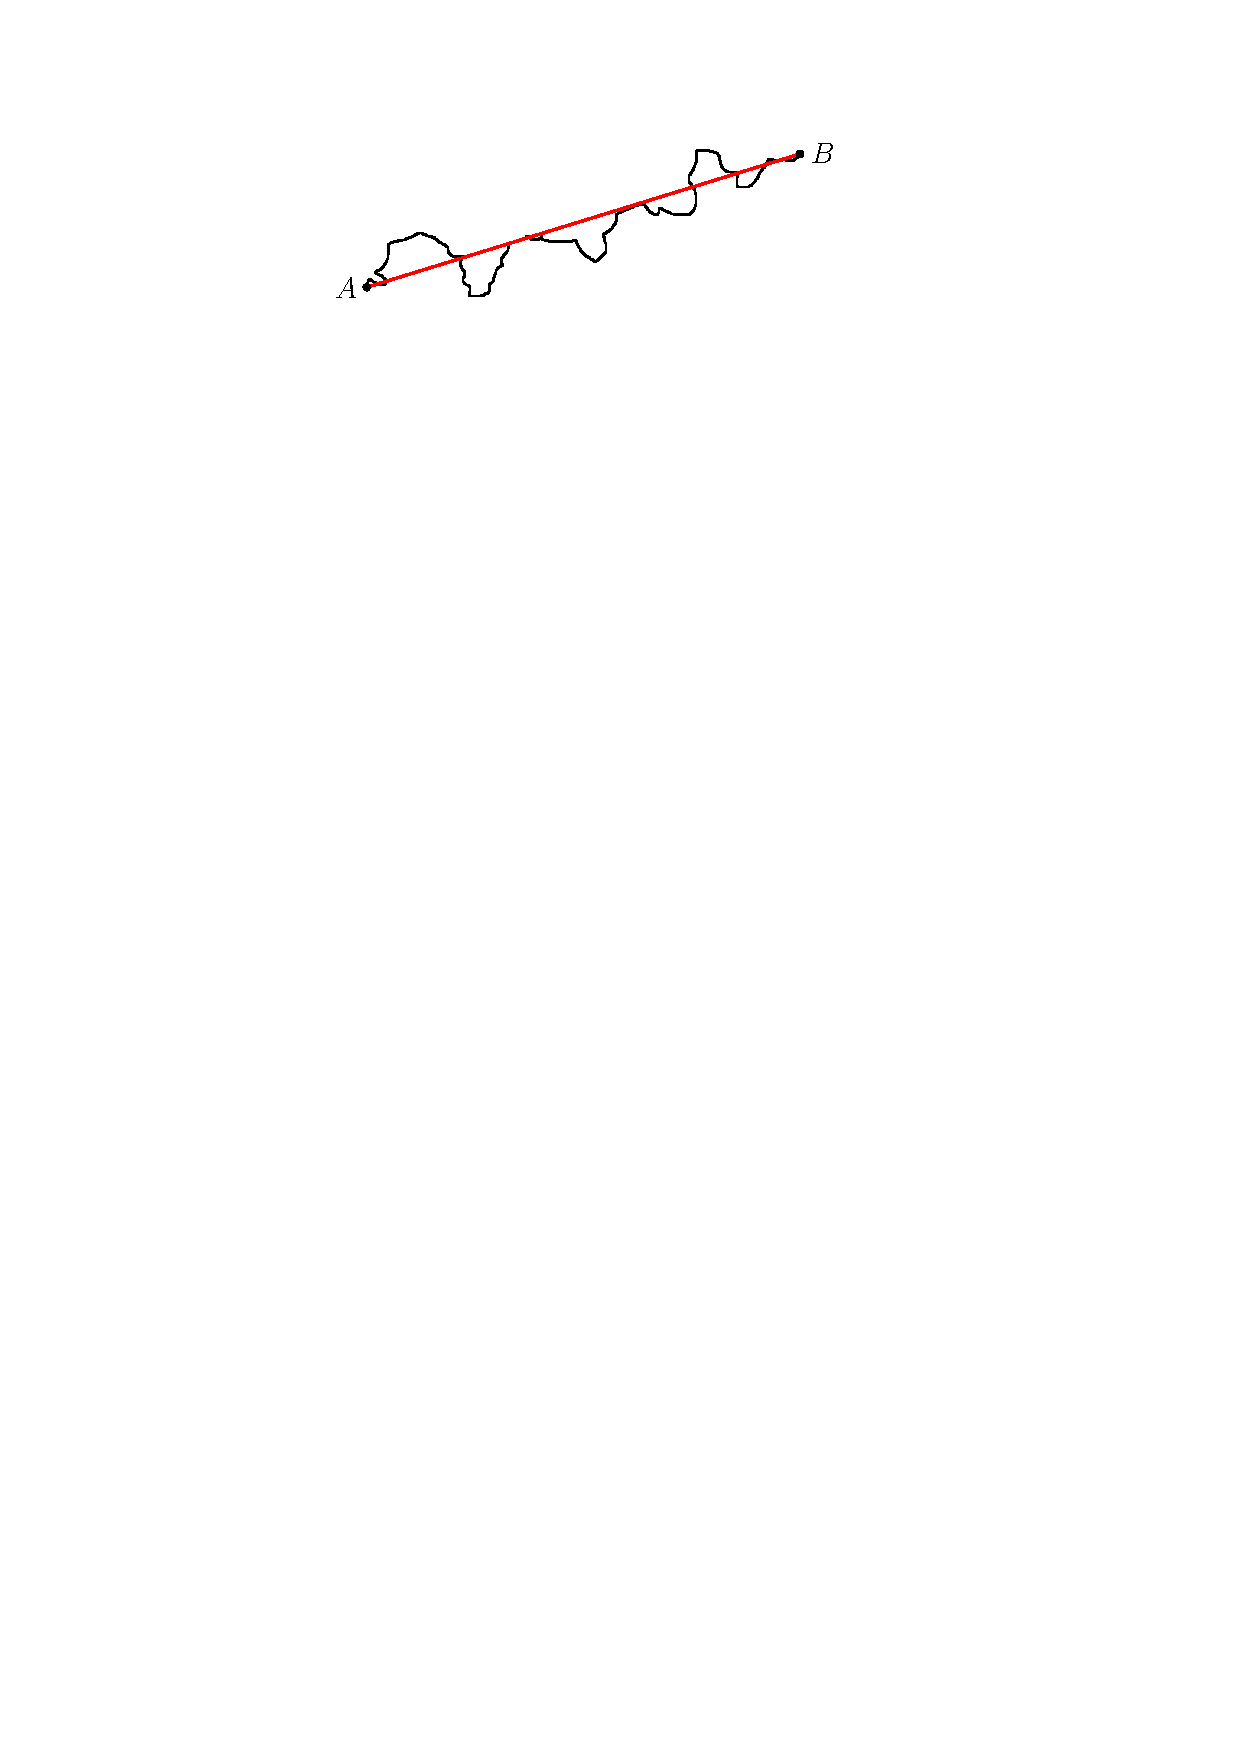
\includegraphics[scale=\normalipe]{ch01-pobrezi.pdf}
    \caption{Příklad mapy pobřeží se spojnicí bodů $A$ a~$B$.}
    \label{fig:pobrezi}
\end{figure}
Zjevně jeho délka je zdola omezena délkou spojnice koncových bodů $A$ a~$B$, nicméně typické pobřeží je velmi nepravidelné a~klikaté. Existují různé metody, které nám umožňují určit jeho délku přesněji. Několik z~nich je popsáno v~knize \citep[str. 79]{Mandelbrot1983}, pro uvedení do problematiky si zde však vystačíme s~tou nejednodušší.\par
Předpokládejme, že pobřeží, které zkoumáme, má pevné hranice (tj. zanedbáváme např. přílivy a~odlivy nastávající během dne), a dále jsme schopni rozlišovat libovolně krátké vzdálenosti.\par
Mějme zadané libovolné $\varepsilon>0$. Podél pobřeží začneme umisťovat tyče tak, že po každém umístění provedeme na mapě krok délky \textbf{nejvýše} $\varepsilon$, přičemž začínáme v~bodě $A$ a~postupujeme až k~bodu $B$ (popř. pokud měříme délku pobřeží ostrova, pokračujeme dokud se nevrátíme tam, kde jsme začali). Předpokládejme, že jsme provedli celkově $n(\varepsilon)$ kroků (jejich počet je závislý na zvolené délce kroku). \emph{Přibližnou délku pobřeží} $\ell(\varepsilon)$ pak stanovíme jako
\begin{equation*}
    \ell(\varepsilon)=n(\varepsilon)\cdot\varepsilon.
\end{equation*}
\begin{figure}[h]
    \centering
    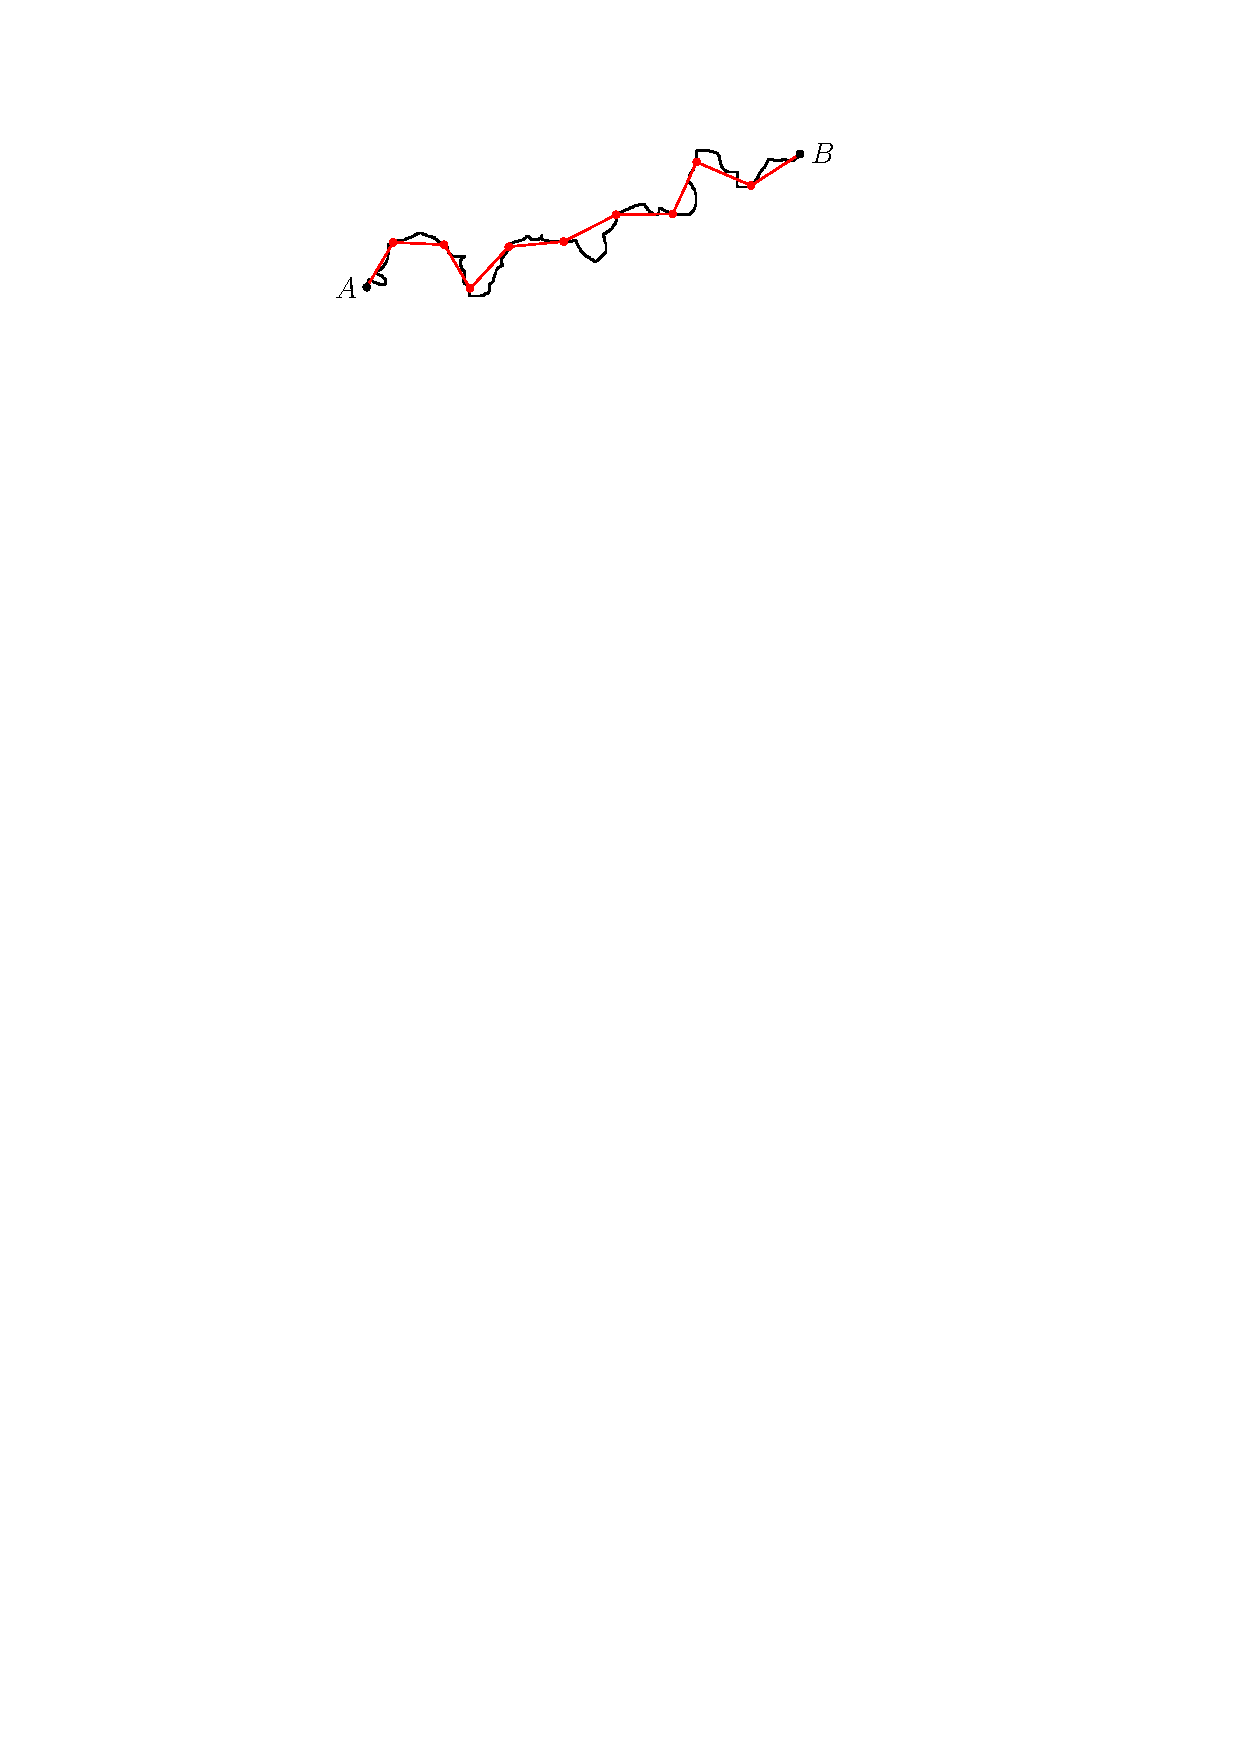
\includegraphics[scale=\normalipe]{ch01-pobrezi-aproximace.pdf}
    \caption{Odhad délky pobřeží, kde $n=10$ při zvoleném $\varepsilon$.}
    \label{fig:pobrezi_aproximace}
\end{figure}
Nyní by nás mohlo napadnout, že pro zmenšující se $\varepsilon$, tj. $\varepsilon\to0_+$, bude hodnota $\ell(\varepsilon)$ konvergovat ke skutečné délce pobřeží. Tzn.~označíme-li skutečnou délku pobřeží $L$, pak bychom mohli očekávat, že platí
\begin{equation}\label{eq:aproximace_limita}
    L=\lim_{\varepsilon\to0_+}{\ell(\varepsilon)}.
\end{equation}
Jenže, bohužel, limita \eqref{eq:aproximace_limita} bude v reálné situaci rovna $\infty$. Proč? Je třeba si uvědomit, že zde pracujeme s~\emph{mapou} pobřeží, která má určité \emph{měřítko}. Pokud bychom měli pobřeží na mapě s~měřítkem $1\,:\,100\;000$, uvidíme méně detailů, než kdybychom jej zkoumali na mapě s~měřítkem $1\,:\,1\;000$. (Viz obrázek~\ref{fig:pobrezi_zoom}.)\par
\begin{figure}[h]
    \centering
    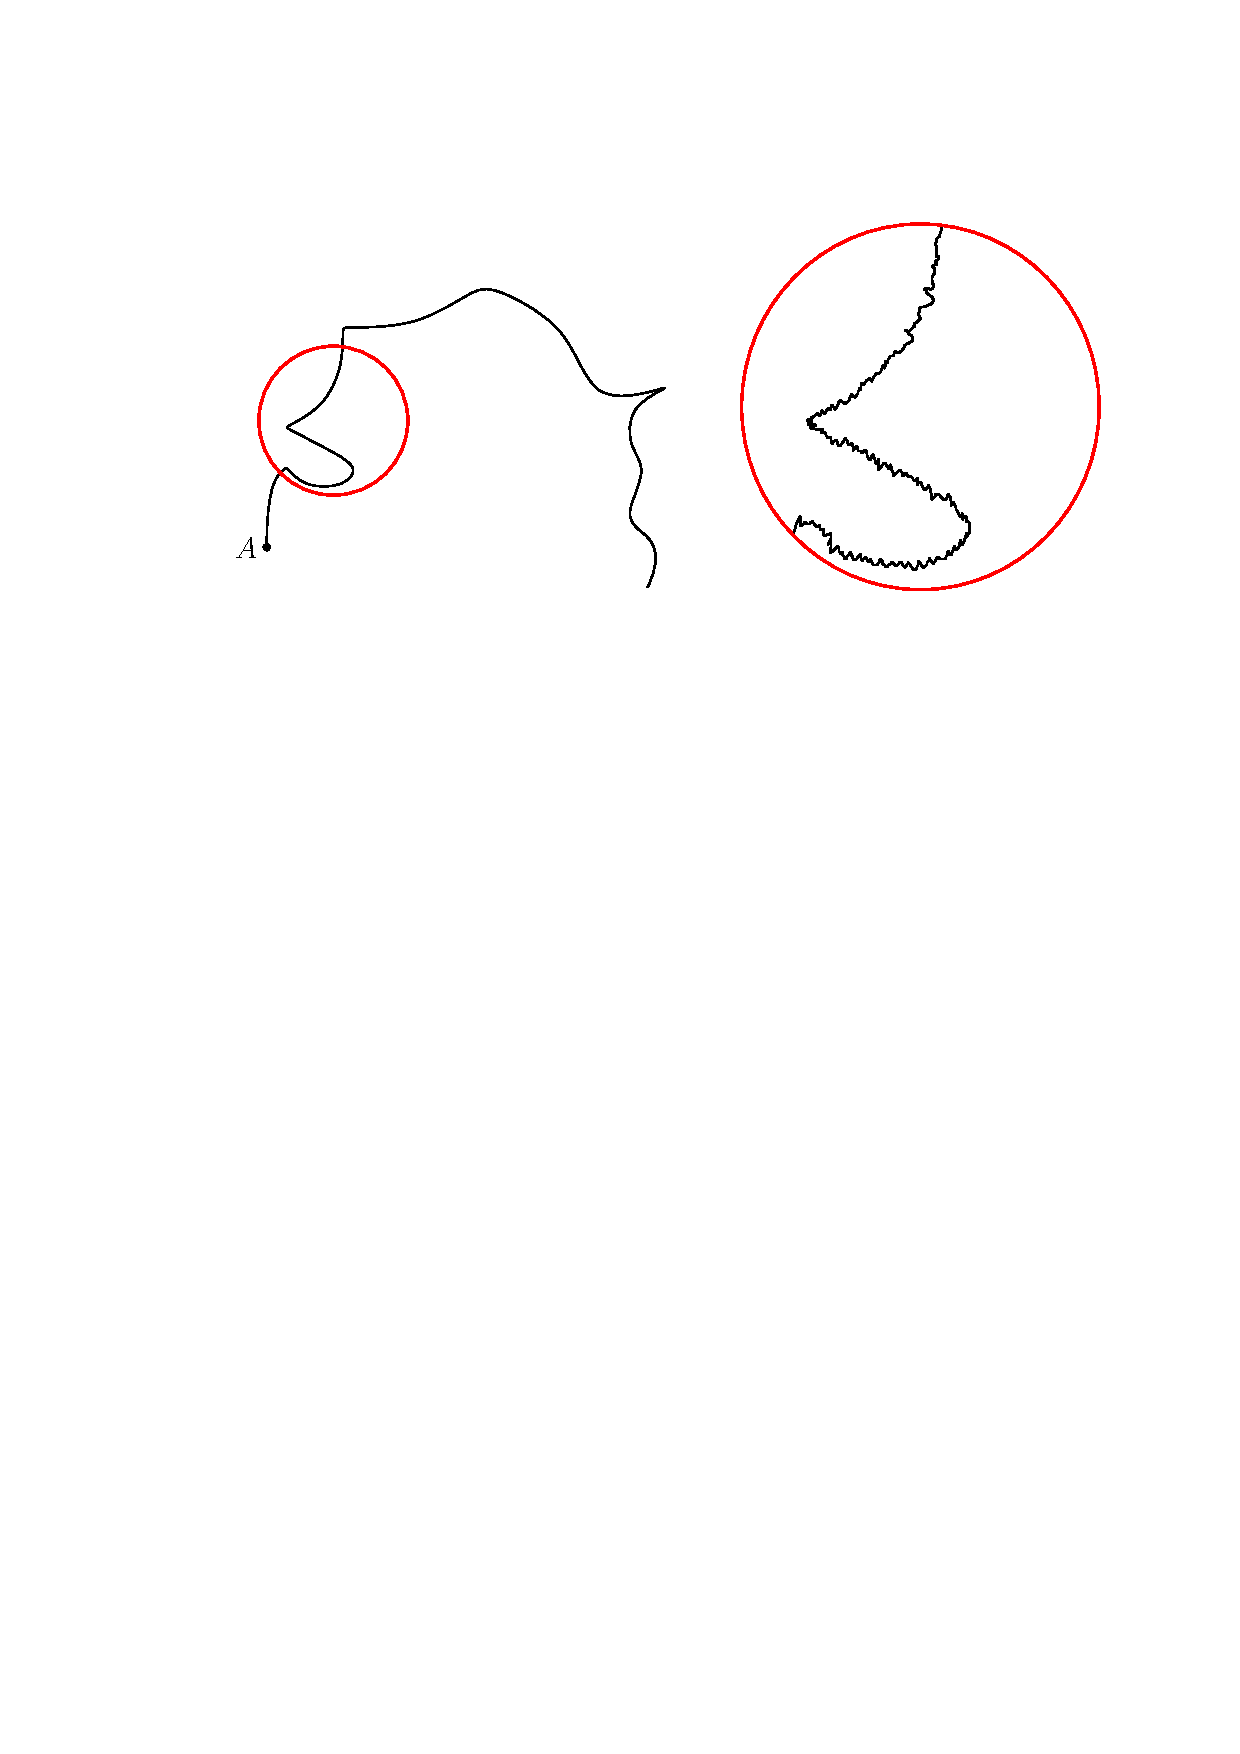
\includegraphics[scale=\normalipe]{ch01-pobrezi-zoom.pdf}
    \caption{Část pobřeží od bodu $A$ v~menším měřítku.}
    \label{fig:pobrezi_zoom}
\end{figure}
Nově odhalené detaily (menší poloostrůvky apod.) zde přispívají k~celkové délce pobřeží $\ell(\varepsilon)$. Postupným zvětšováním měřítka mapy bychom tak odhalili další detaily. Naše původní idea tak selhává, neboť (v "klasickém" pojetí délky) pro $\varepsilon\to0_+$ hodnota $\ell(\varepsilon)$ patrně poroste nade všechny meze, tj. $\lim_{\varepsilon\to0_+}{\ell(\varepsilon)}=\infty$.\par
Nabízí se otázka: Proč se toto děje? Pokud se ohlédneme zpět za eukleidovskou geometrií\index{geometrie!eukleidovská}\index{eukleidovská geometrie}, tento problém v ní nenastává. Např. u~kružnice v~eukleidovské rovině $\mathbb{E}_2$ změnou měřítka žádné další detaily křivky neobjevíme (podobně u~jiných geometrických útvarů, viz obrázky~\ref{subfig:kruznice} a~\ref{subfig:kruznice_zoom}). 
\begin{figure}[h]
    \centering
    \begin{subfigure}{\subfigwidth}
        \centering
        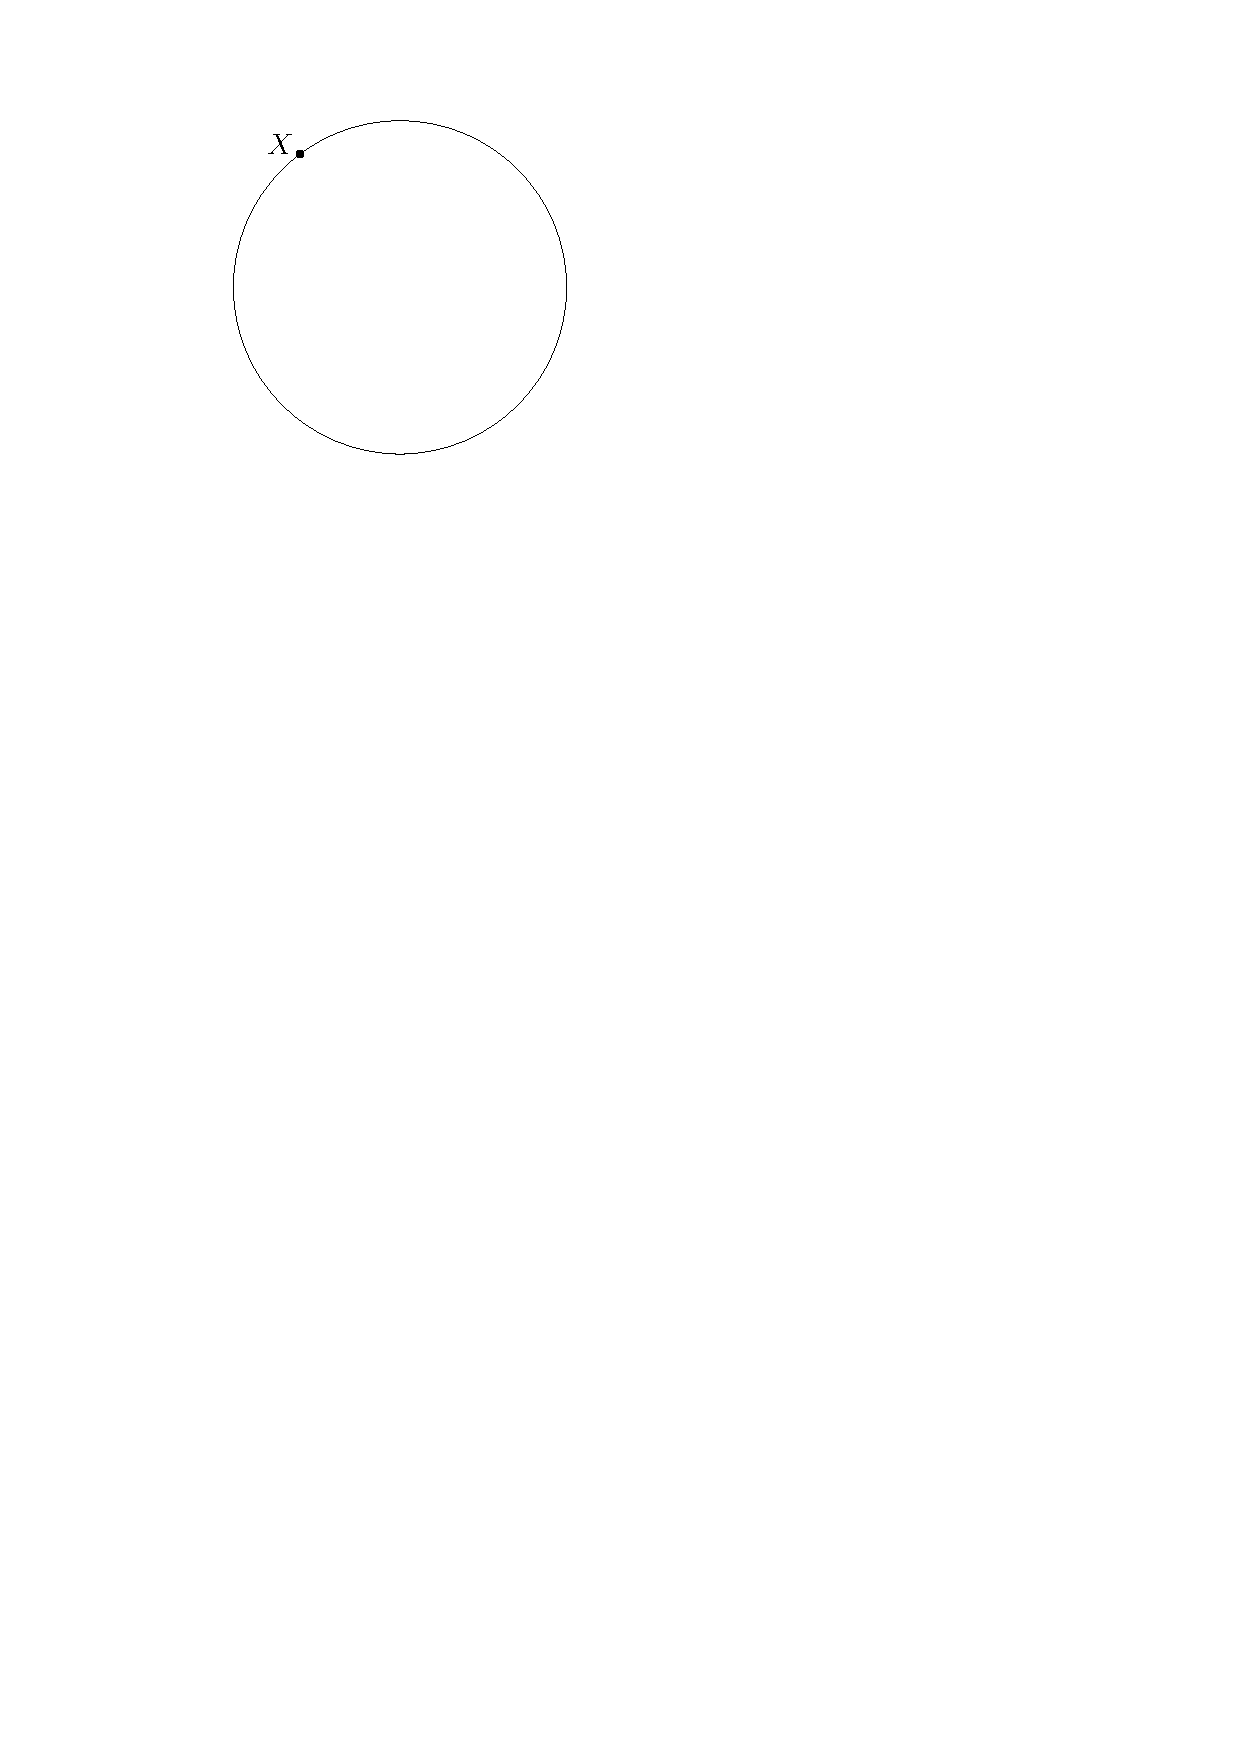
\includegraphics[scale=\normalipe]{ch01-kruznice.pdf}
        \caption{Kružnice v~menším měřítku.}
        \label{subfig:kruznice}
    \end{subfigure}
    \quad
    \begin{subfigure}{\subfigwidth}
        \centering
        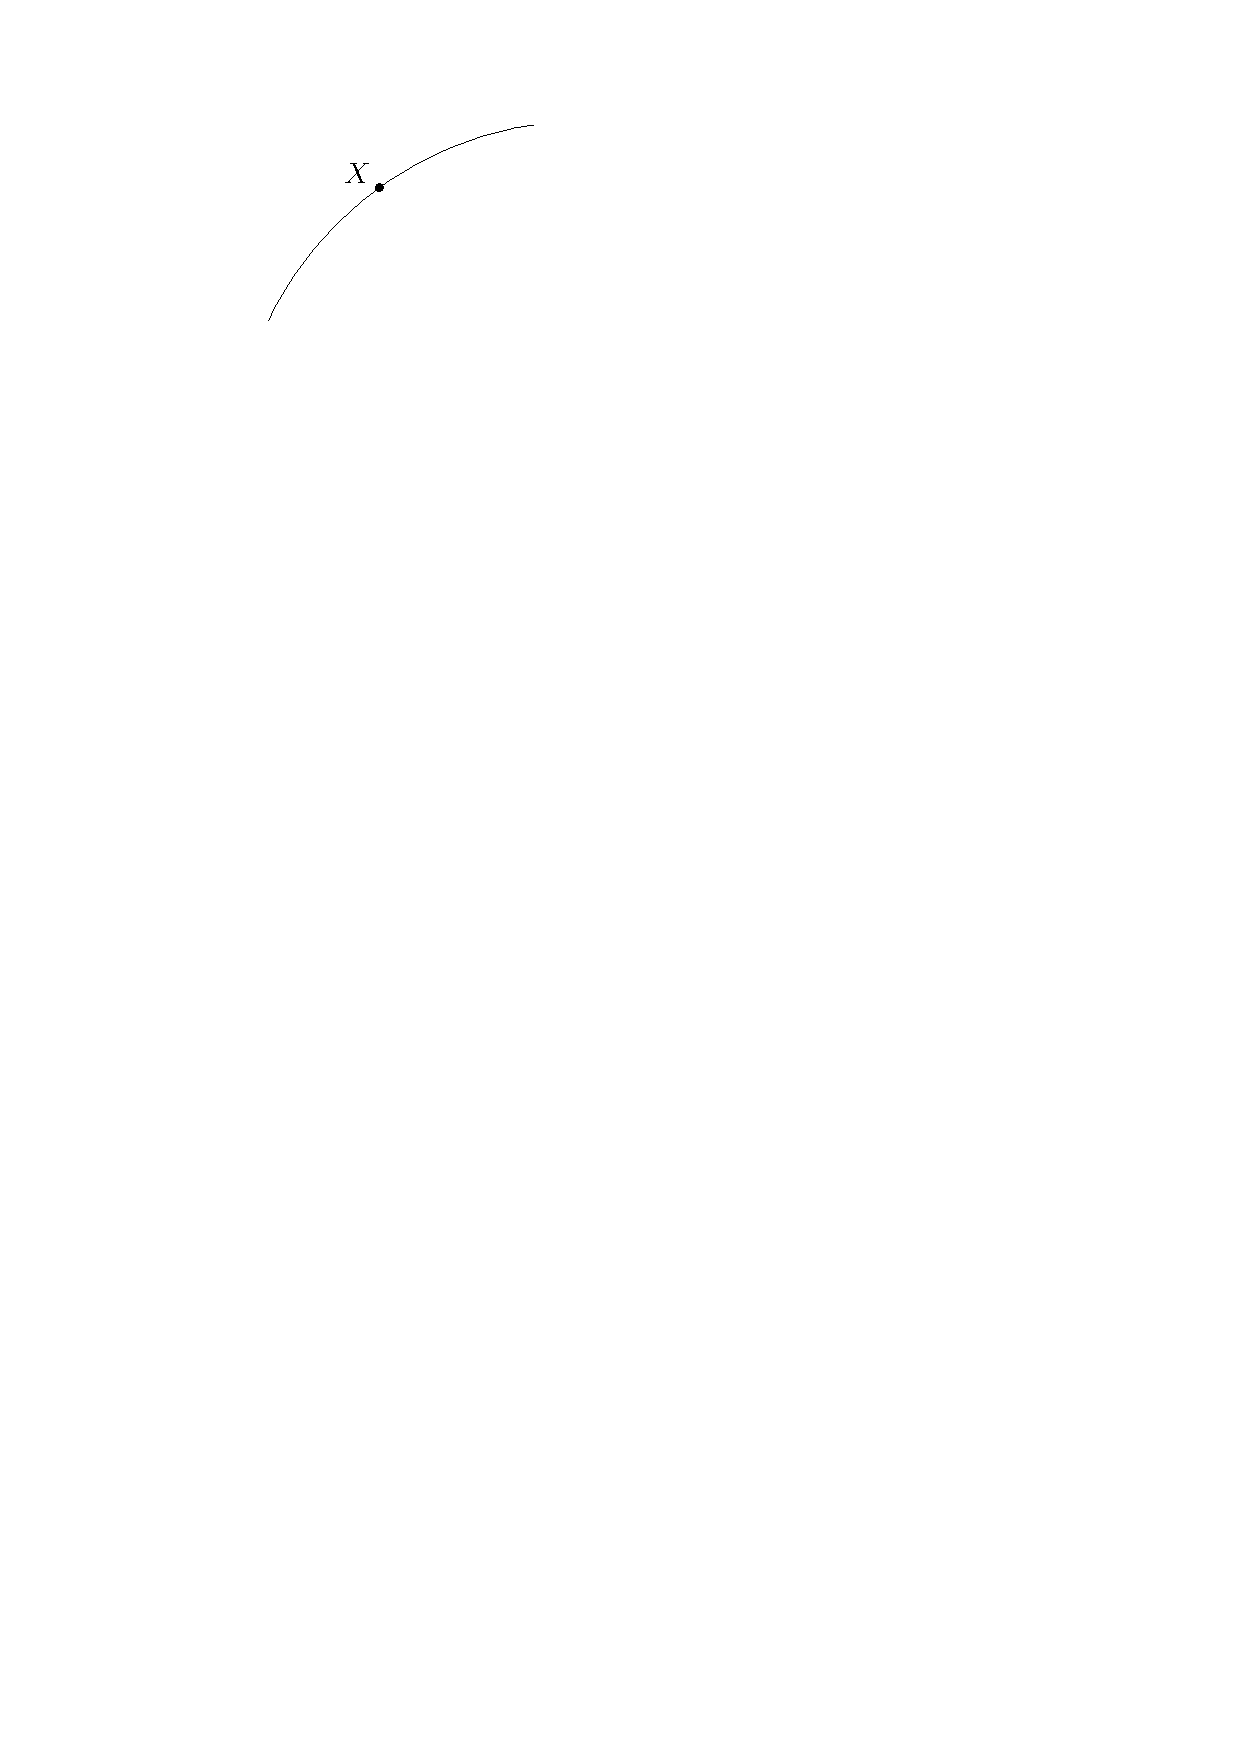
\includegraphics[scale=\normalipe]{ch01-kruznice-zoom.pdf}
        \caption{Část kružnice ve větším měřítku.}
        \label{subfig:kruznice_zoom}
    \end{subfigure}
\end{figure}
Díky tomu můžeme v~případě počítání obvodu kružnice použít následující postup.\par
Máme-li kružnici o~poloměru $r>0$, pak jí můžeme vepsat libovolný pravidelný $n$-úhelník (viz obrázek~\ref{subfig:archimedova_metoda}).
\begin{figure}[h]
    \centering
    \begin{subfigure}{\subfigwidth}
        \centering
        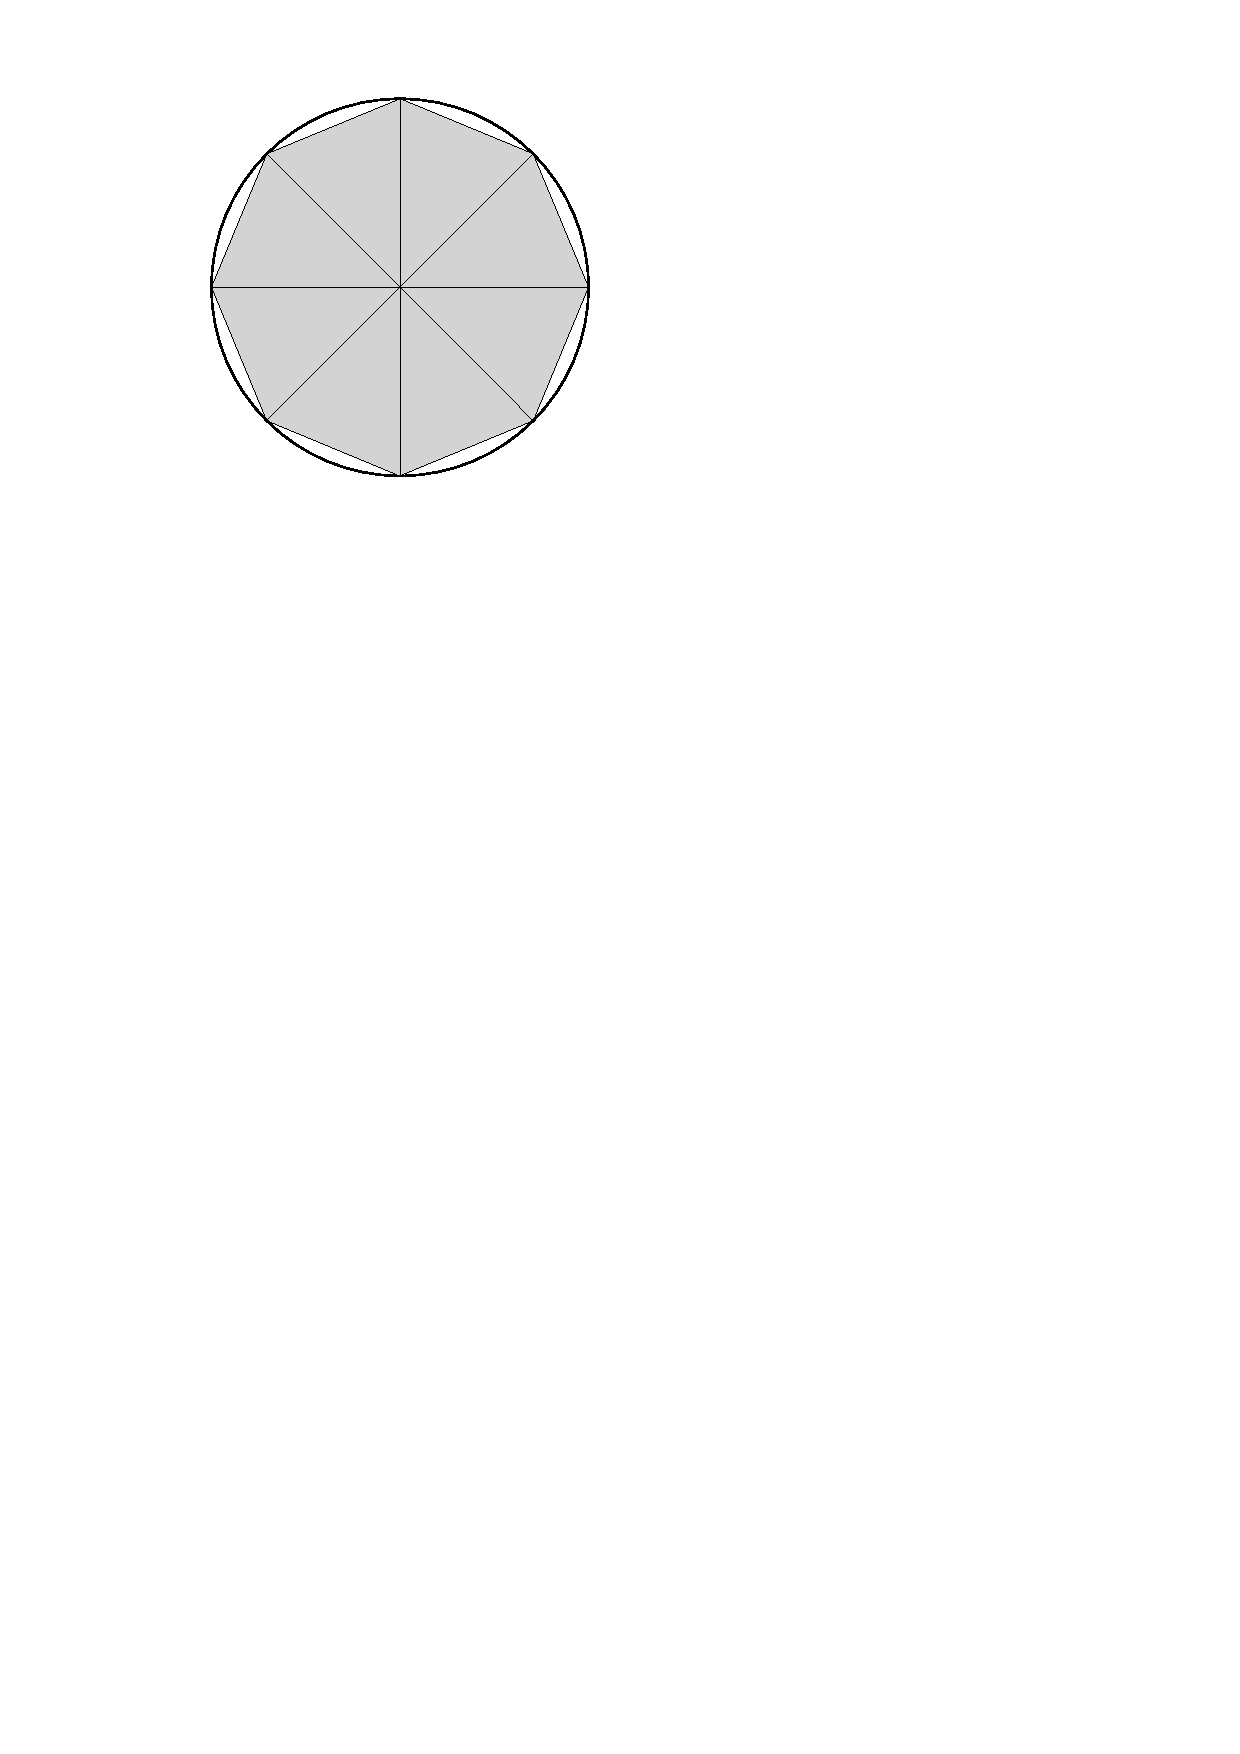
\includegraphics[scale=\normalipe]{ch01-archimedova-metoda.pdf}
        \caption{Pravidelný osmiúhelník vepsaný kružnici.}
        \label{subfig:archimedova_metoda}
    \end{subfigure}
    \quad
    \begin{subfigure}{\subfigwidth}
        \centering
        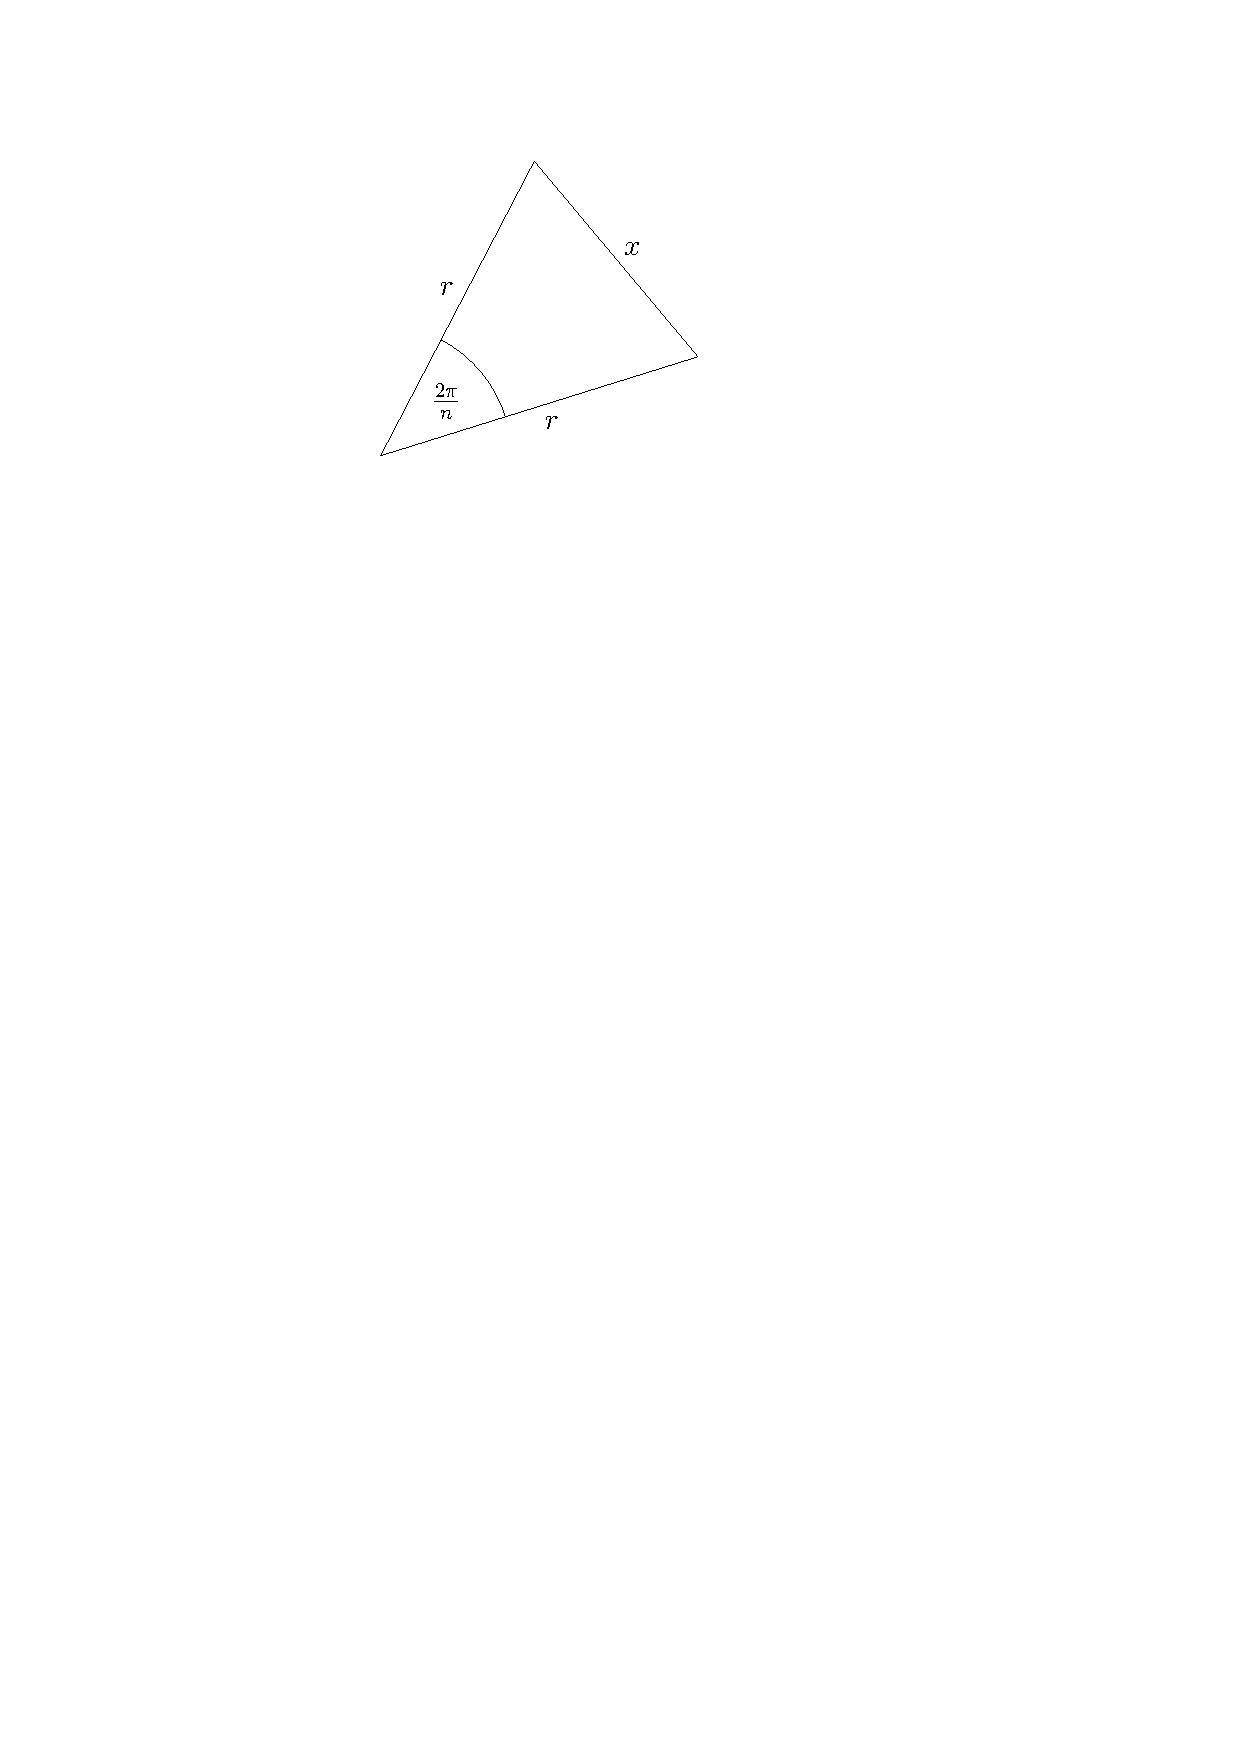
\includegraphics[scale=\normalipe]{ch01-archimedova-metoda-cast-nuhelniku.pdf}
        \caption{Část vepsaného pravidelného $n$-úhelníku.}
        \label{subfig:archimedova_metoda_cast_nuhelniku}
    \end{subfigure}
    \caption{Princip Archimédovy metody.}
    \label{fig:princip_archimedovy_metody}
\end{figure}
Obvod pravidelného $n$-úhelníku is označíme $O_n$ a~délku jeho strany $x$ (viz obrázek~\ref{subfig:archimedova_metoda_cast_nuhelniku}). Tu jsme schopni stanovit užitím elementární goniometrie, tj.
\begin{equation*}
    x=2r\cdot\sin{\dfrac{\pi}{n}},
\end{equation*}
a tedy obvod
\begin{equation*}
    O_n=2rn\cdot\sin{\dfrac{\pi}{n}}.
\end{equation*}
Pro rostoucí $n$ bude obvod pravidelného $n$-úhelníku stále lépe aproximovat obvod původní kružnice (viz obrázek~\ref{fig:archimedova_metoda_presnejsi}).
\begin{figure}[h]
    \centering
    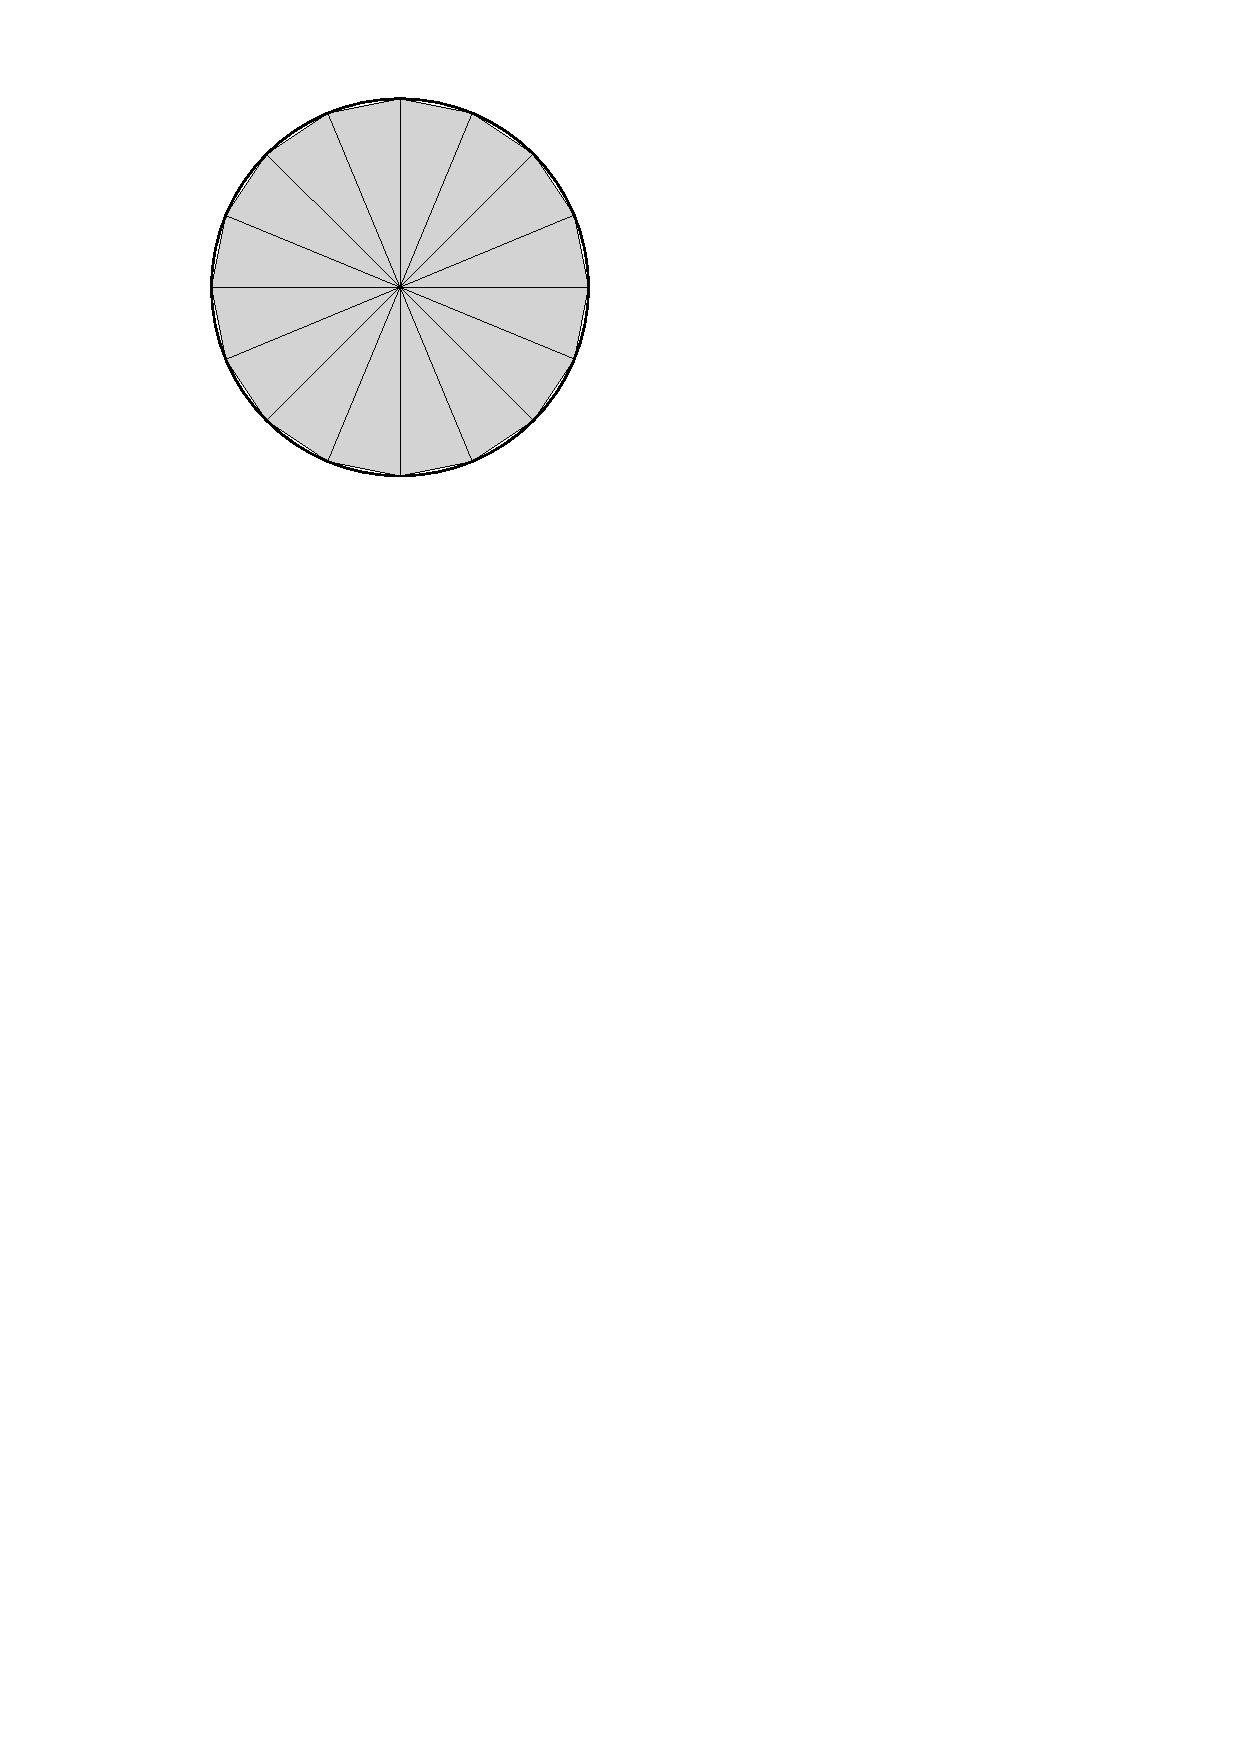
\includegraphics[scale=\normalipe]{ch01-pobrezi-aproximace-presnejsi.pdf}
    \caption{Aproximace obvodu kružnice pomocí pravidelného šestnáctiúhelníku.}
    \label{fig:archimedova_metoda_presnejsi}
\end{figure}
Limitním přechodem (tj. pro $n\to\infty$) tak můžeme odvodit vzorec pro obvod kružnice:
\begin{align*}
    O&=\lim_{n\to\infty}{2rn\cdot\sin{\dfrac{\pi}{n}}}=2r\cdot\lim_{n\to\infty}{n\cdot\sin{\dfrac{\pi}{n}}}=2\pi r\cdot\lim_{n\to\infty}{\cdot\dfrac{\sin{\dfrac{\pi}{n}}}{\dfrac{\pi}{n}}}=2\pi r.
\end{align*}
Idea aproximace pomocí "zjemňování" zde skutečně funguje a~délka ve standardním pojetí tak dává smysl, jak bychom mohli očekávat. Křivka, kterou tvoří pobřeží, má však oproti kružnici jiný geometrický charakter. Délka pobřeží $\infty$, k~níž Mandelbrot došel, tak dává smysl \emph{z geometrického pohledu}, avšak výsledek to není moc užitečný.
\section{Soběpodobnost}\label{sec:sobepodobnost}
Mandelbrot si uvědomil,~že struktura pobřeží se charakterově vymyká útvarům do tehdy známým eukleidovské geometrii,~neboť mapy s~různými měřítky poskytovaly různou úroveň detailů,~které hrály netriviální roli v~jeho celkové délce. Učinil však jiné zásadní pozorování,~a to sice,~že mnoho detailů má společné rysy,~které se opakují. Hodně z~nich se shodovalo s~výjimkou jejich měřítka. \citep[str. 96]{Mandelbrot1983}\par

Ve fraktální geometrii se pro tento úkaz uchytil termín \emph{soběpodobnost} (angl. \emph{self-similarity}). Útvar nazýváme soběpodobným,~\textbf{pokud se sám sobě podobný v~libovolném měřítku} \citep[str. 220]{Voracova2022} nebo pokud \textbf{část útvaru je podobná jeho celku}. Zmíněná podoba může být míněna přibližně (např. v~případě pobřeží je nejspíše jasné,~že žádné z~jeho detailů nesdílejí společné rysy přesně),~ale v~dalších částech si předvedeme soběpodobnost \emph{přímou}\index{soběpodobnost}.

\subsection{Kochova křivka}\label{subsec:kochova_krivka}
Jak jsme si již uvedli,~za otce fraktální geometrie je považován Mandelbrot,~avšak mnoho fraktálních křivek bylo známo již dříve (čtenář promine,~že jsme blíže nespecifikovali termín "fraktální",~jeho přesný význam pro nás však zatím nebude stěžejní). Jako první se podíváme na jednu z~nejznámějších,~kterou objevil roku \emph{1904} švédský matematik \name{Helge~von~Koch} \mbox{(1870--1924)},~dnes známou pod~názvem \emph{Kochova křivka}\index{Kochova křivka}\index{křivka!Kochova}. \citep[str. 61]{Peitgen2004} Na začátku vezmeme úsečku délky $1$. Vyjmeme prostřední (tj. druhou) třetinu a nahradíme ji dvěma úsečkami délky $1/3$,~tak,~aby na sebe navazovaly v~krajních bodech. Tento proces následně opakujeme pro nově vzniklé úsečky. Obecně u~úsečky délky $l$ nahradíme její prostřední třetinu dvojicí úseček délek $l/3$ (viz obrázek \ref{fig:kochova_vlocka_5iteraci}).
\begin{figure}[h]
    \centering
    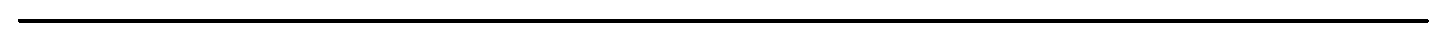
\includegraphics[scale=\fractalscale]{ch01-kochova-krivka-0iterace.pdf}\\\qquad\\
    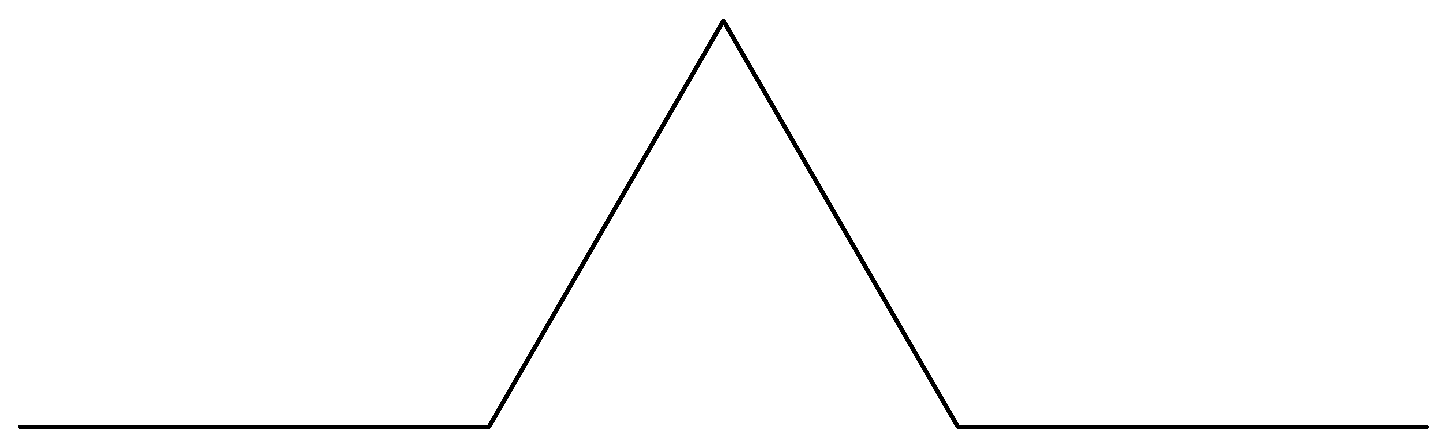
\includegraphics[scale=\fractalscale]{ch01-kochova-krivka-1iterace.pdf}\\\qquad\\
    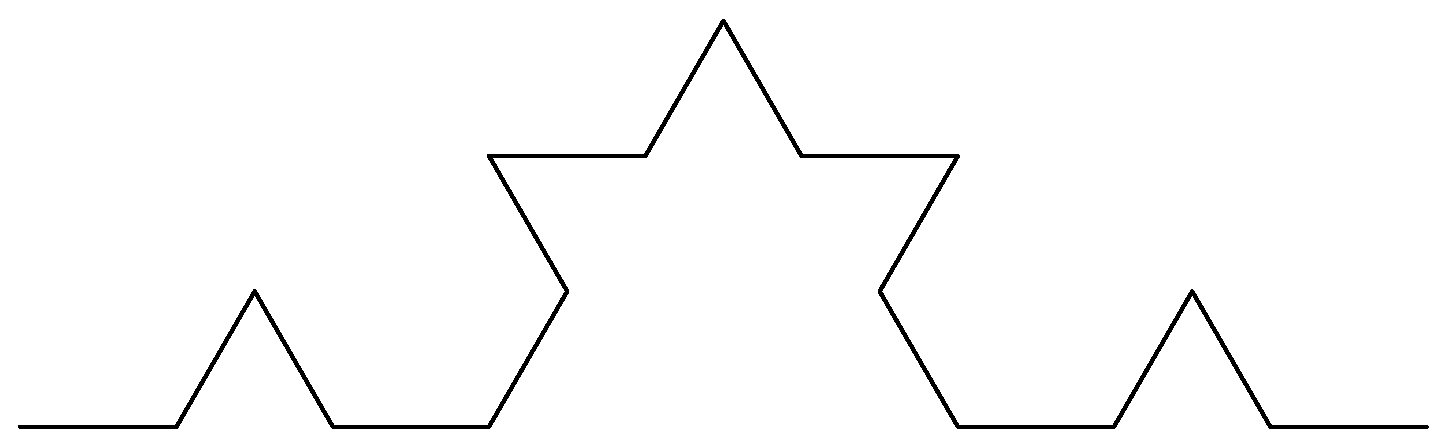
\includegraphics[scale=\fractalscale]{ch01-kochova-krivka-2iterace.pdf}\\\qquad\\
    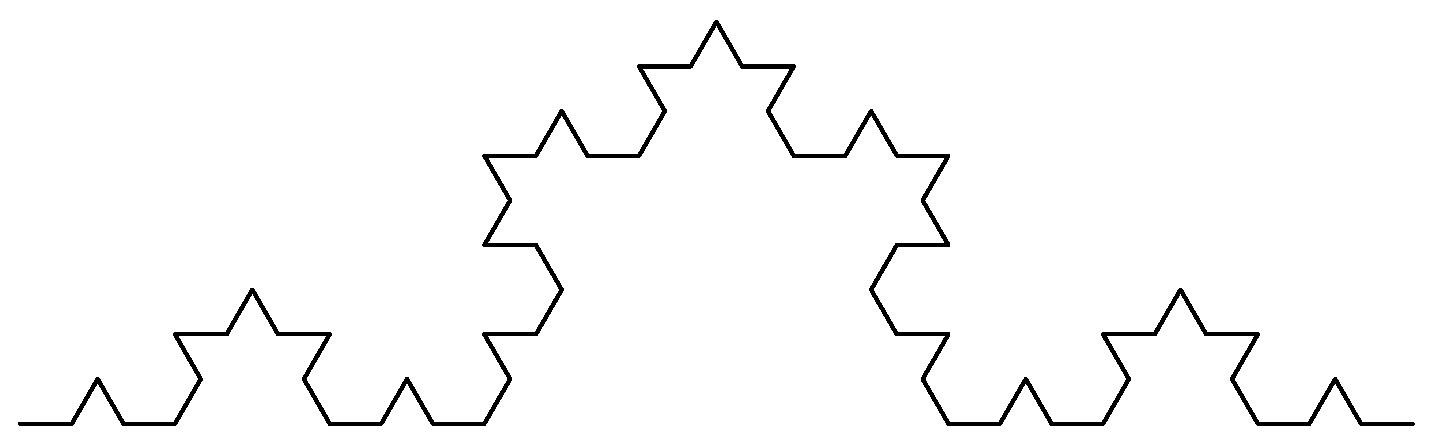
\includegraphics[scale=\fractalscale]{ch01-kochova-krivka-3iterace.pdf}\\\qquad\\
    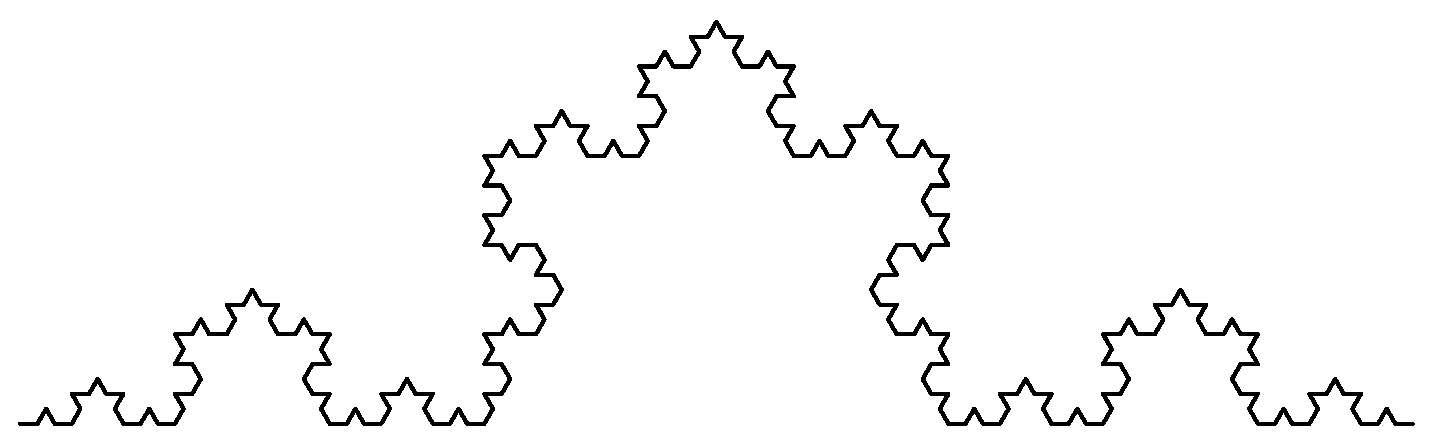
\includegraphics[scale=\fractalscale]{ch01-kochova-krivka-4iterace.pdf}\\\qquad\\
    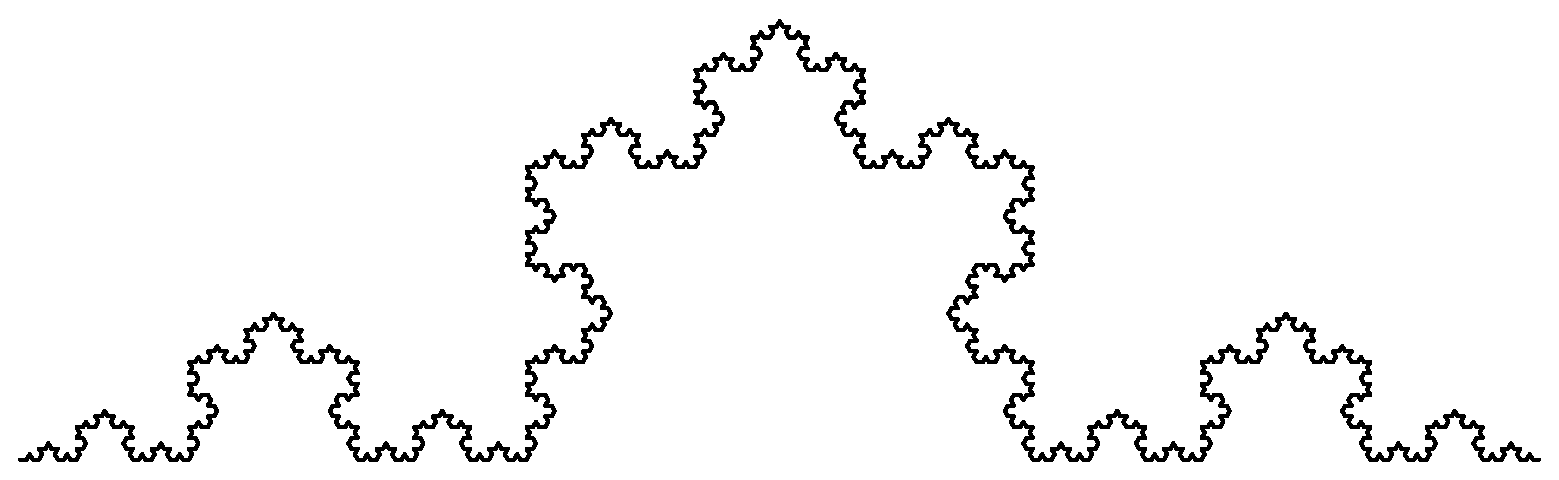
\includegraphics[scale=\fractalscale]{ch01-kochova-krivka-5iterace.pdf}
    \caption{Prvních pět iterací Kochovy křivky.}
    \label{fig:kochova_vlocka_5iteraci}
\end{figure}
V první řadě si můžeme všimnout,~že v~každé další iteraci jsou nově vzniklé podobné původnímu celku,~tedy v~předešlé iteraci (viz obrázek \ref{fig:kochova_krivka_podobnost}). Pokud by tento proces pokračoval do nekonečna,~pak by každá ze čtyř částí křivky představovala \textbf{celý původní obrazec} ve zmenšeném měřítku (byla by tedy soběpodobná).
\begin{figure}[h]
    \centering
    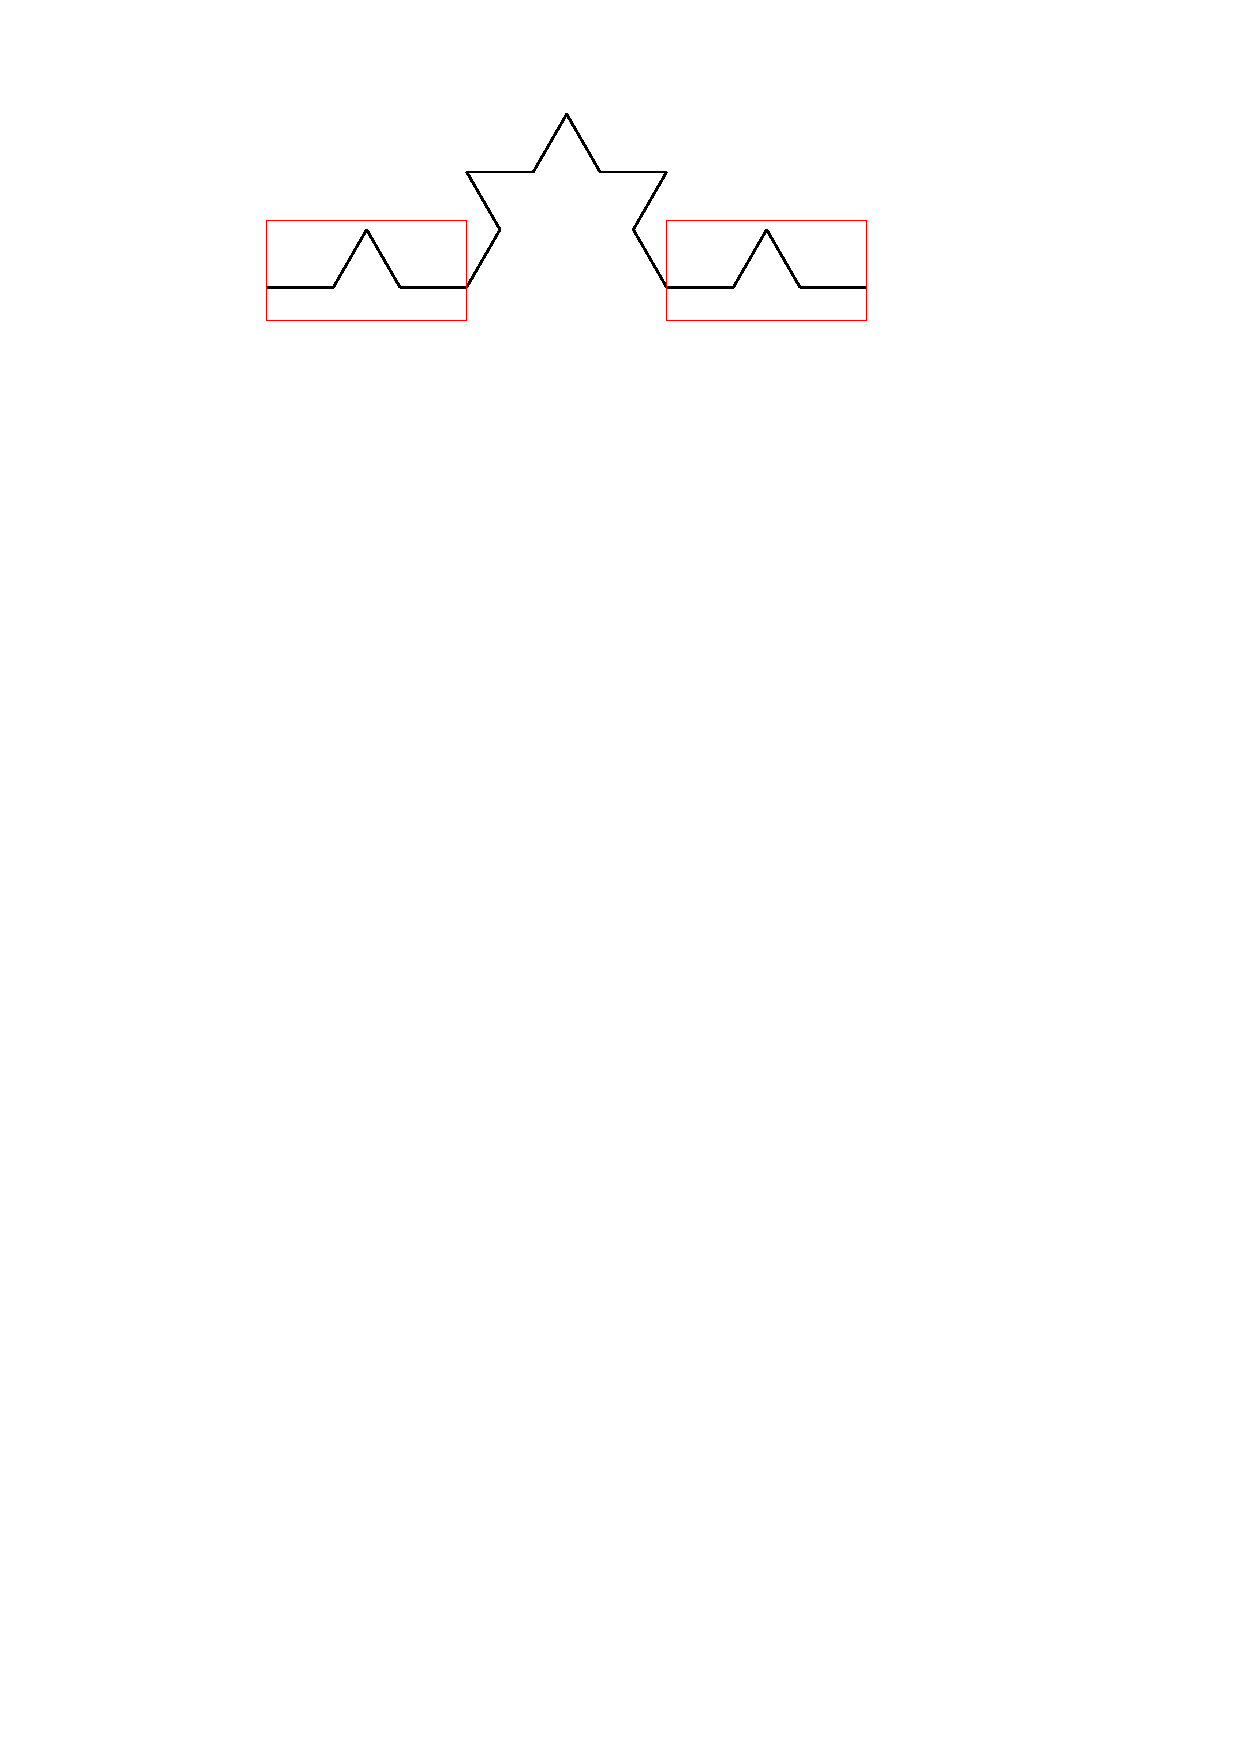
\includegraphics[scale=\normalipe]{ch01-kochova-krivka-podobnost.pdf}
    \caption{První iterace Kochovy křivky "uvnitř" druhé v~menším měřítku.}
    \label{fig:kochova_krivka_podobnost}
\end{figure}
Zkusme se nyní podívat na délku křivky. V~první iteraci začínáme s~úsečkou délky\footnote{Mohli bychom také začít s~obecnou délkou $\ell_0$,~ale ta by se však při výpočtu projevila pouze jako konstantní násobek.} $1$,~která se v~druhé iteraci změní na křivku délky $4/3$. Není těžké si rozmyslet,~že obecně v~$n$-té iteraci bude délka křivky $\ell_n$ rovna
\begin{equation*}
    \left(\dfrac{4}{3}\right)^{n}.
\end{equation*}
Posloupnost $\{\ell_n\}_{n=1}^{\infty}$ je geometrická s~kvocientem $q=4/3>1$,~a tedy její limita je $\infty$. Kochova křivka má tak \emph{nekonečnou délku}.

\subsection{Sierpińského trojúhelník}\label{subsec:sierpinskeho_trojuhelnik}
Přesuneme nyní k~plošným útvarům,~neboť i~zde lze sledovat některé zajímavé vlastnosti. Jedním z~představitelů je tzv. \emph{Sierpińského trojúhelník}\index{Sierpińského trojúhelník}\index{trojúhelník!Sierpińského},~který objevil roku \emph{1916} polský matematik \name{Wacław~Sierpiński} \mbox{(1882--1969)}. \citep[str. 61]{Peitgen2004} Na začátku (v nulté iteraci) začínáme s~rovnostranným trojúhelníkem se stranou délky $1$ (též lze začít s~obecnou délkou $\ell_0$). V~něm sestrojíme střední příčky (tj. spojnice středů stran trojúhelníka),~které společně utvoří strany rovnostranného trojúhelníka\index{trojúhelník!rovnostranný}\index{rovnostranný trojúhelník} čtvrtinového obsahu původního trojúhelníka (to vychází z~faktu,~že střední příčka v~libovolném trojúhelníku má délku rovnou polovině délky strany,~s~níž je rovnoběžná). Obsah nově vzniklého trojúhelníku odebereme a postup opakujeme pro zbývající trojici trojúhelníků v~původním obrazci (viz obrázek \ref{fig:sierpinskeho-trojuhelnik-5iteraci}).\par
\begin{figure}[h]
    \centering
    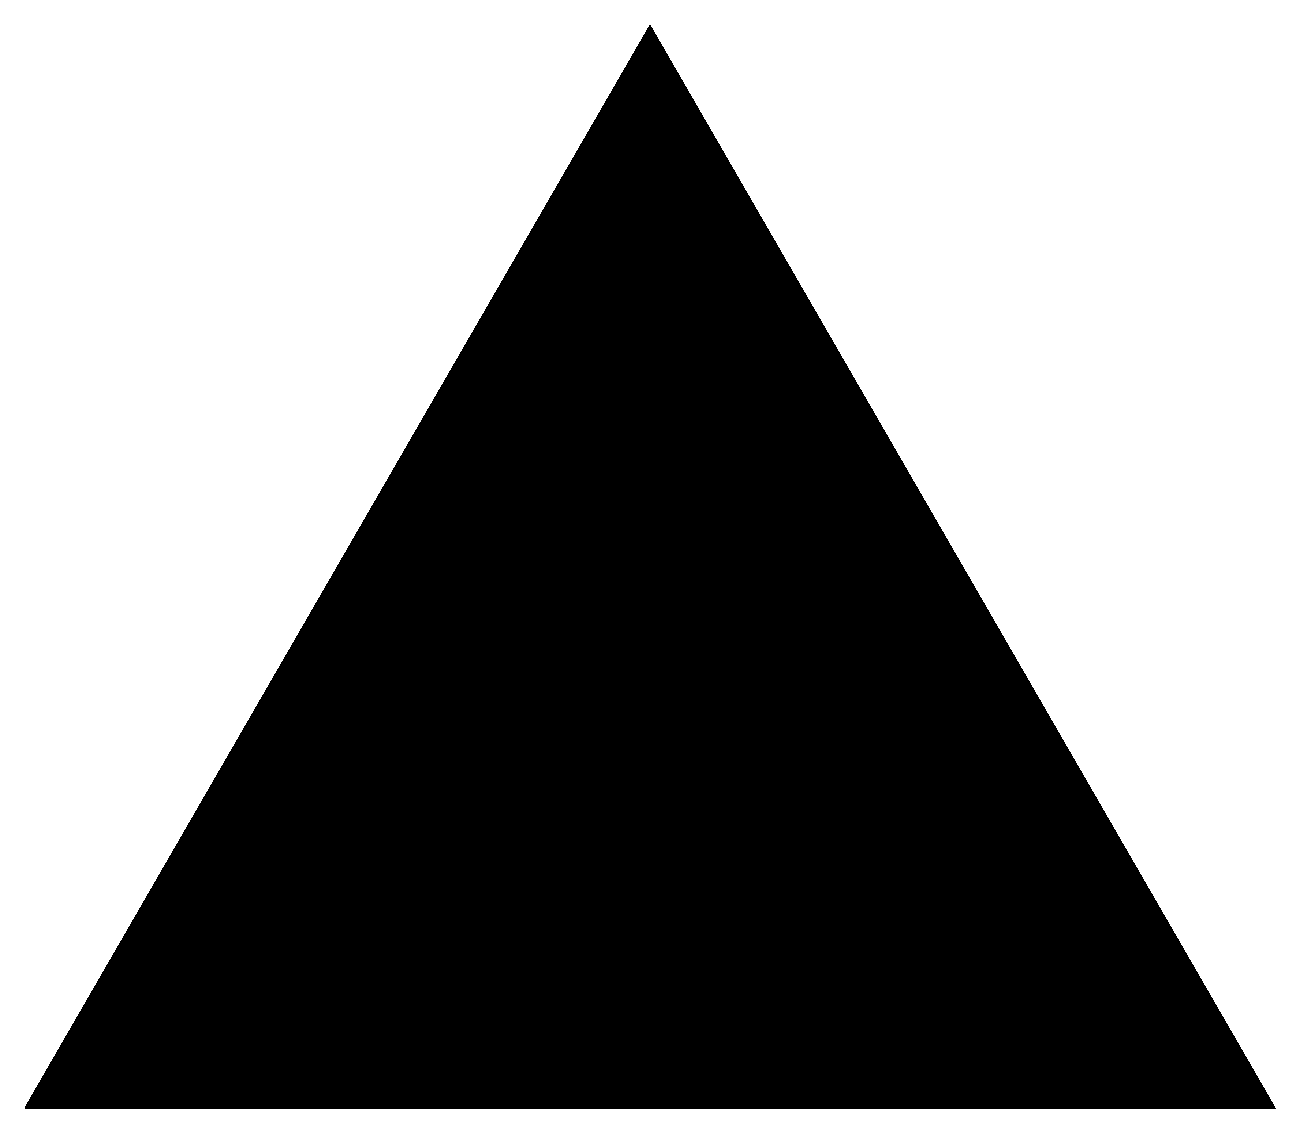
\includegraphics[width=0.4\textwidth]{ch01-sierpinskeho-trojuhelnik-0iterace.pdf}\qquad
    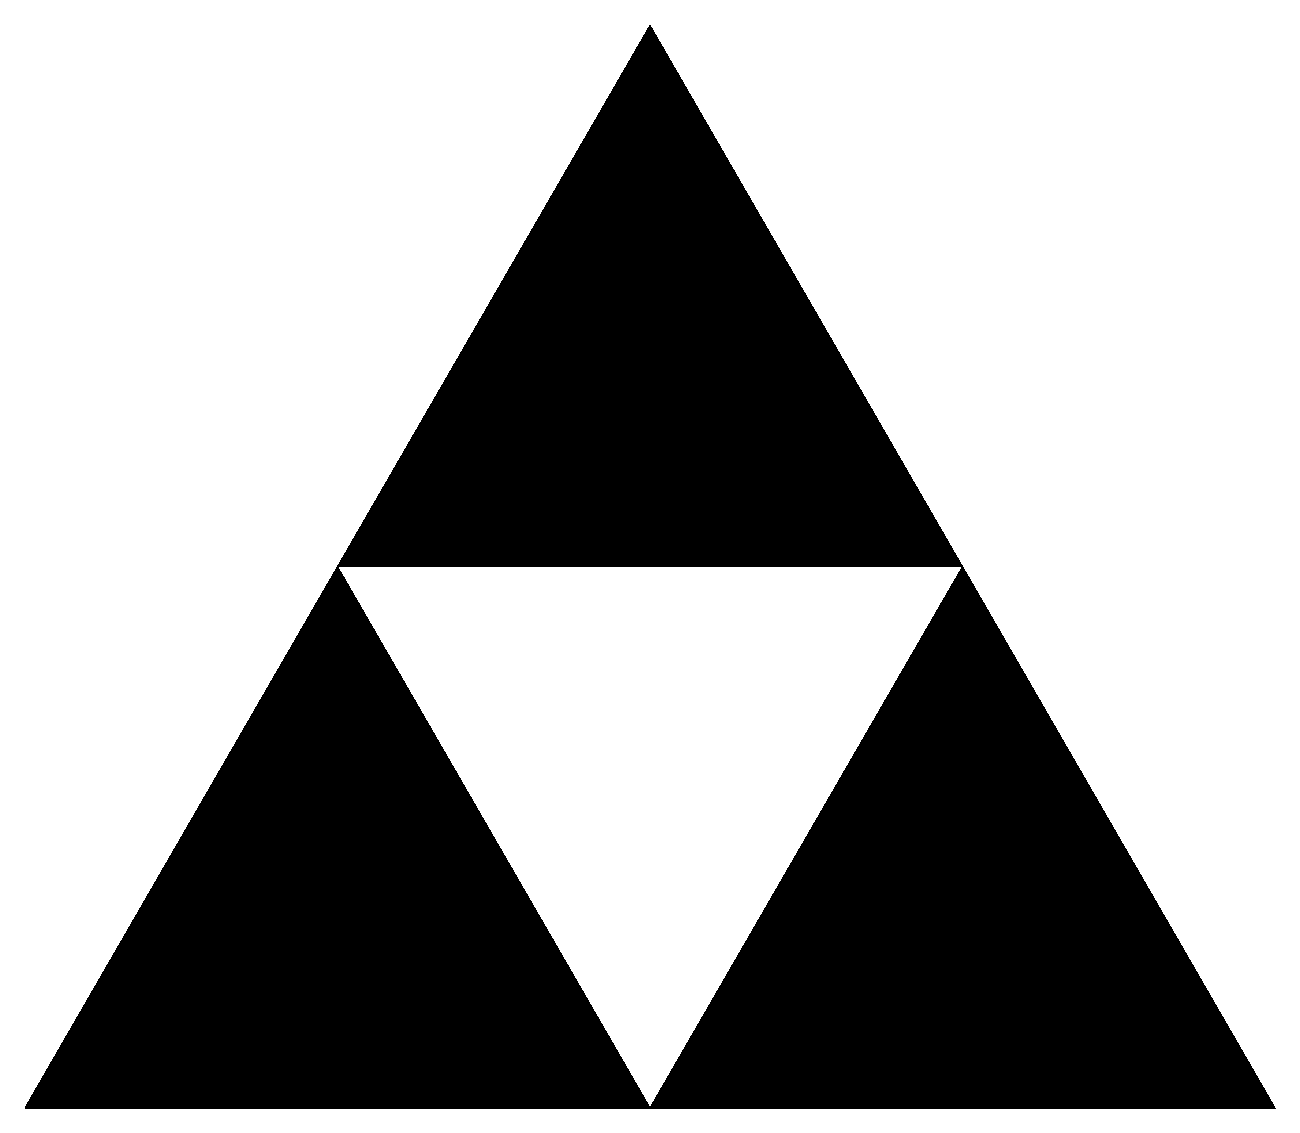
\includegraphics[width=0.4\textwidth]{ch01-sierpinskeho-trojuhelnik-1iterace.pdf}\qquad\\
    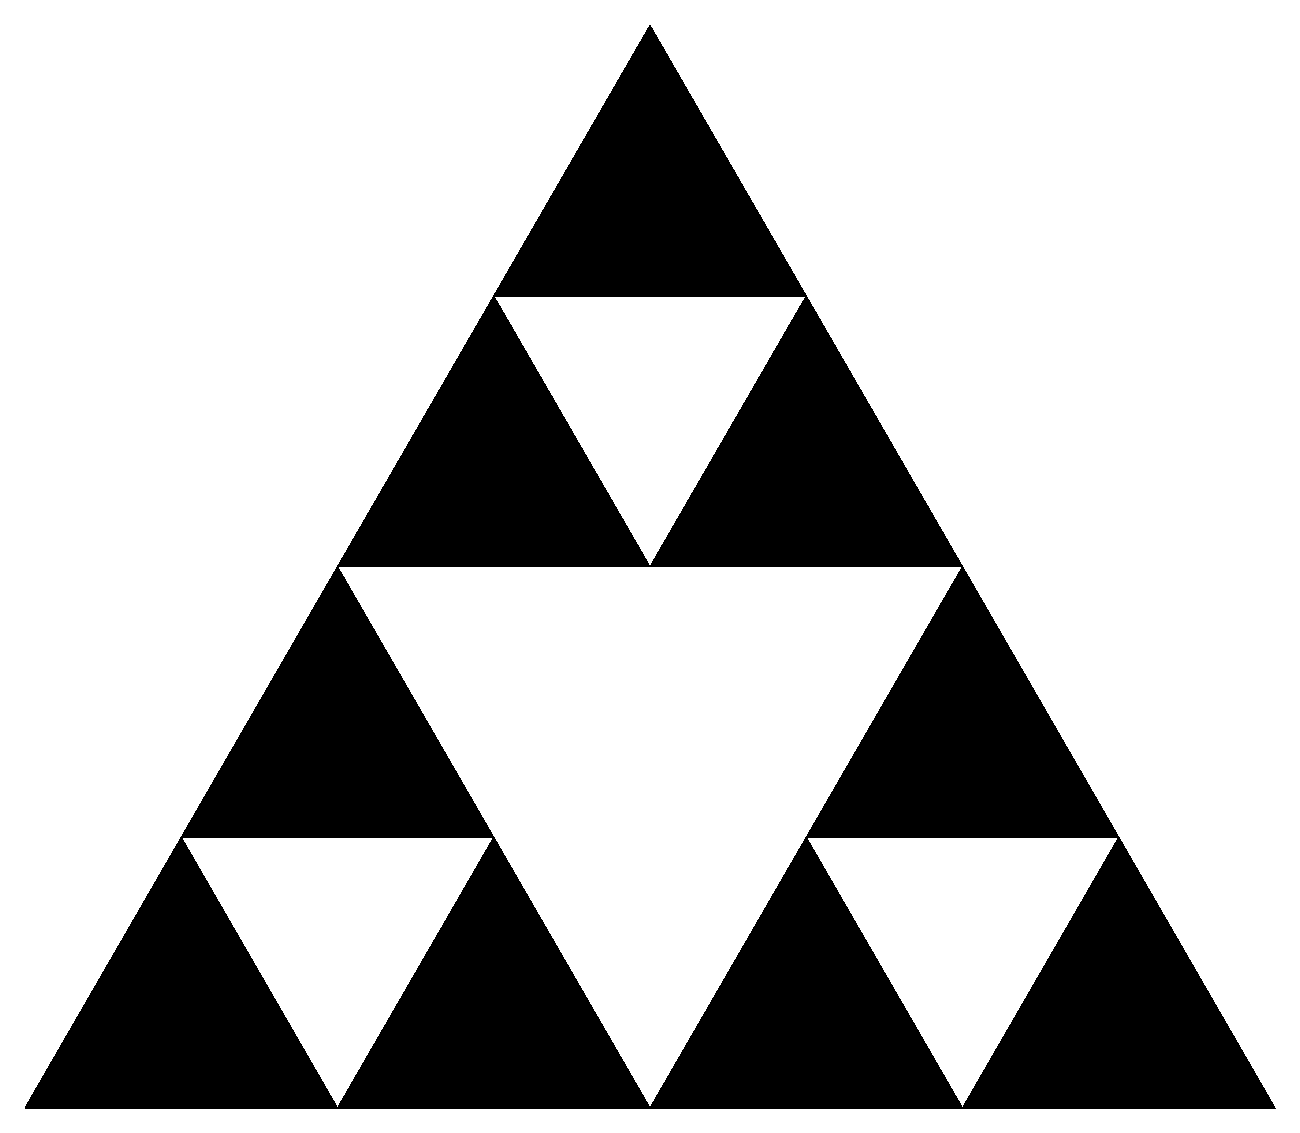
\includegraphics[width=0.4\textwidth]{ch01-sierpinskeho-trojuhelnik-2iterace.pdf}\qquad
    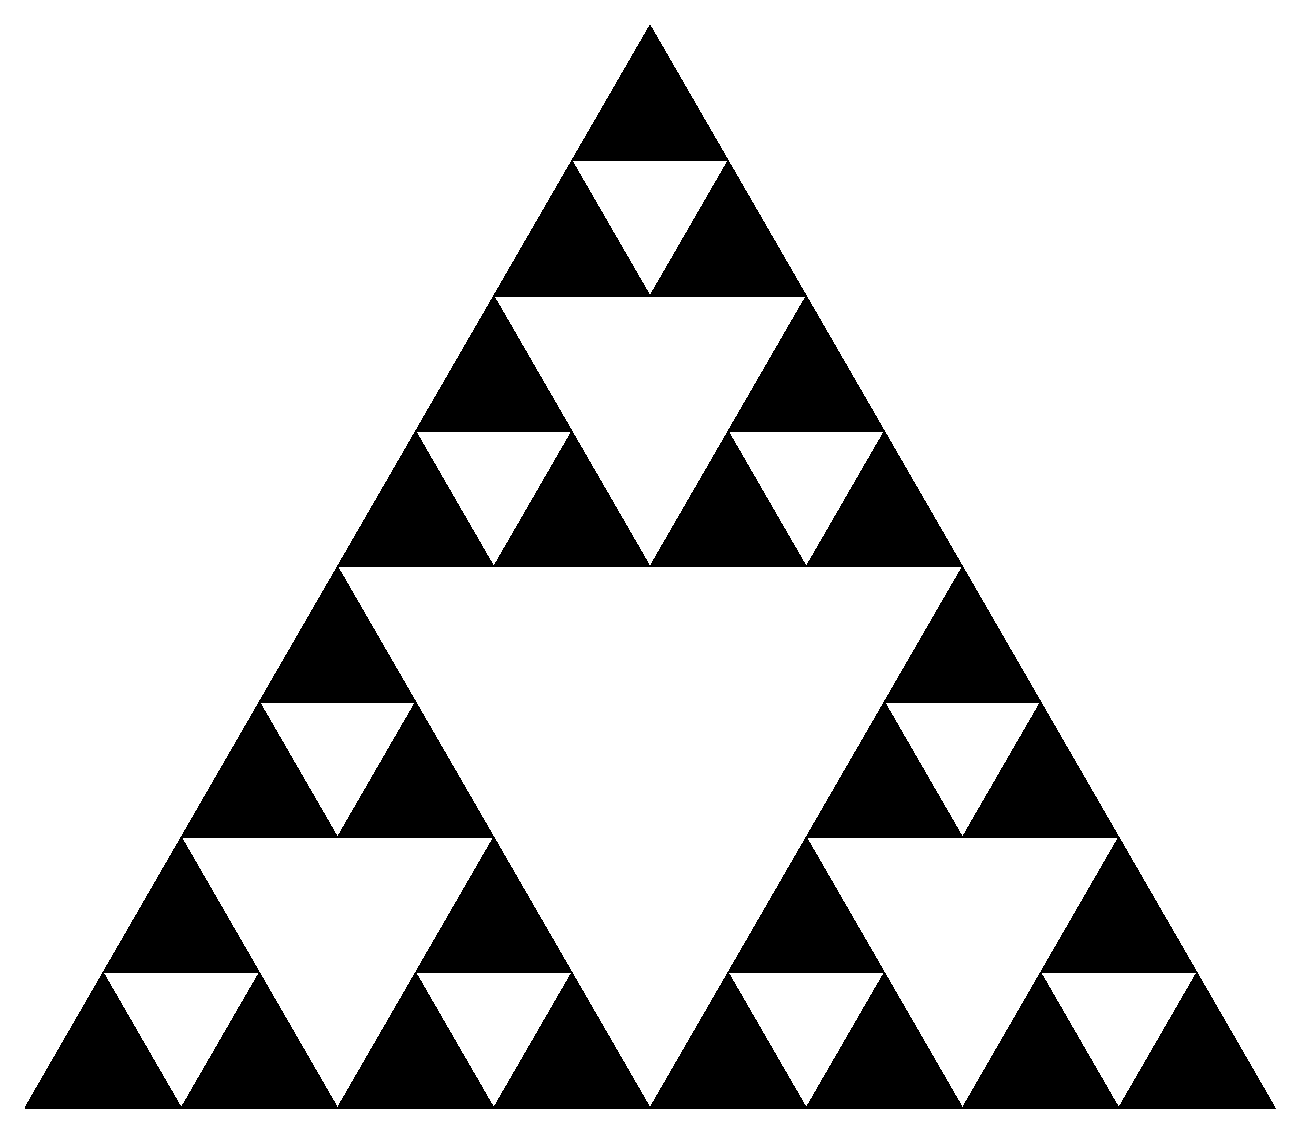
\includegraphics[width=0.4\textwidth]{ch01-sierpinskeho-trojuhelnik-3iterace.pdf}\qquad\\
    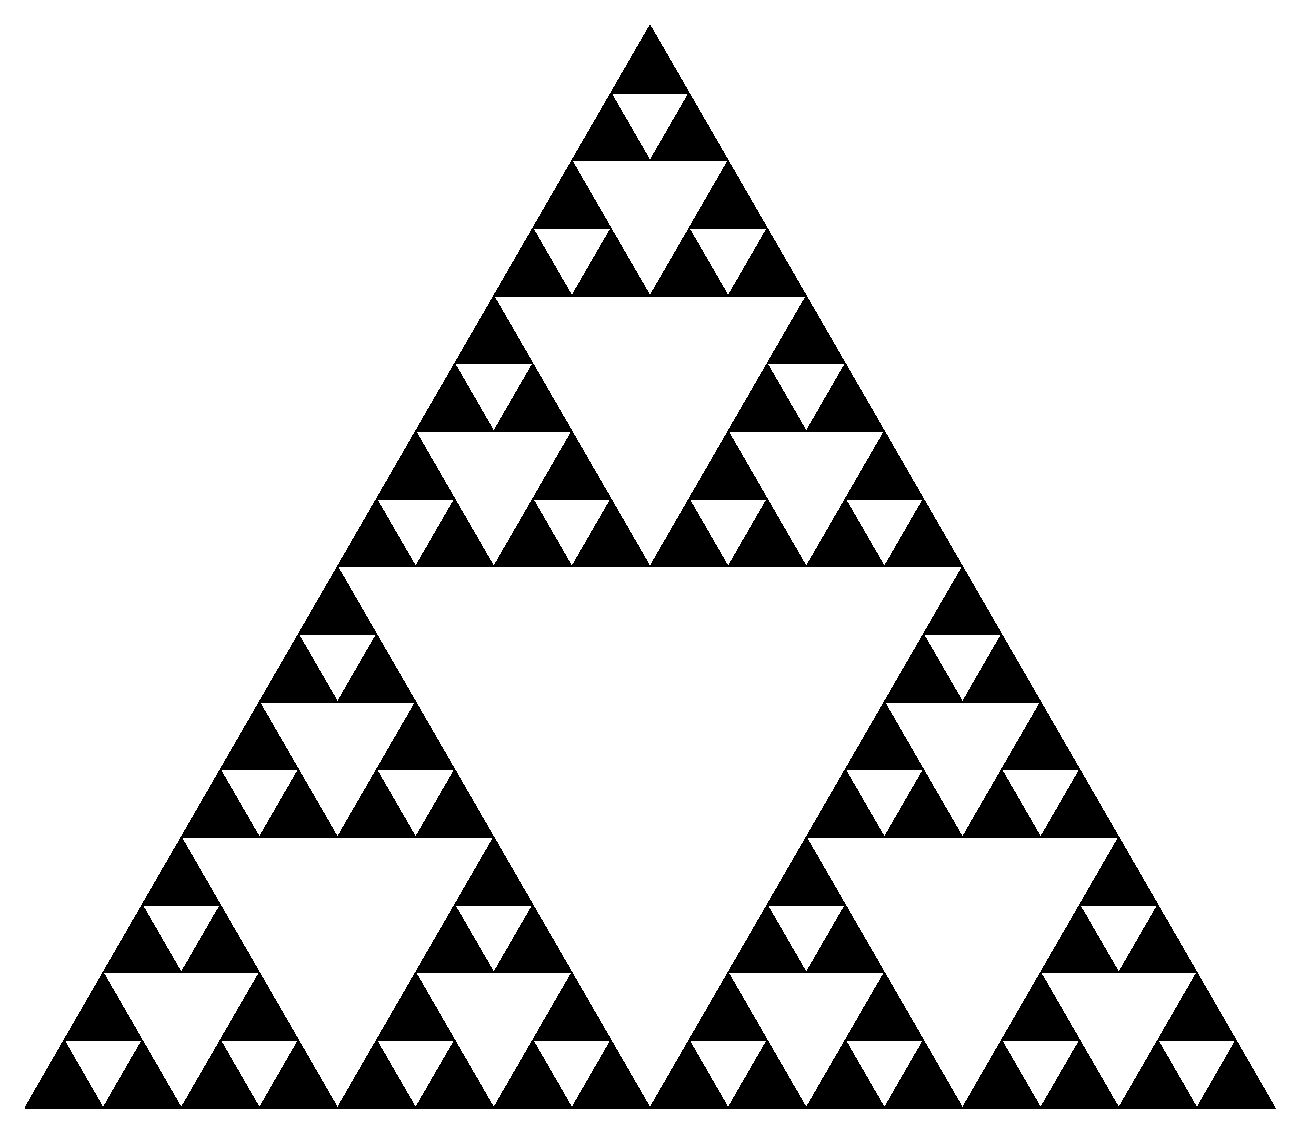
\includegraphics[width=0.4\textwidth]{ch01-sierpinskeho-trojuhelnik-4iterace.pdf}
    \caption{První čtyři iterace Sierpińského trojúhelníka.}
    \label{fig:sierpinskeho-trojuhelnik-5iteraci}
\end{figure}
I zde si lze všimnout,~že po nekonečně mnoha iteracích budou menší trojúhelníky přesnými kopiemi původního obrazce. Zkusme se opět podívat,~jak je to s~obvodem obrazce. Každá ze středních příček,~které vzniknou v~další iteraci,~má poloviční délku vůči délce strany $l$ původního trojúhelníku. Obvod obrazce se tak zvětší o~$3l/2$. Počet trojúhelníků poroste exponenciálně,~neboť v~každé iteraci odstraněním jednoho trojúhelníku vzniknou tři nové,~tj. obvod se po $k$-té iteraci zvětší o~$3^k\cdot(1/2)^k=(3/2)^k$ (na začátku pro $k=0$ je obvod $3$). Obvod obrazce $O_n$ po $n$ iteracích bude roven součtu přírůstků přes všechny iterace,~tj.
\begin{equation}\label{eq:obvod_sierpinskeho_trojuhelniku_niteraci}
    O_n=3+\sum_{k=1}^n{\left(\dfrac{3}{2}\right)^k}.
\end{equation}
Řada $\sum_{k=1}^{n}(3/2)^k$ je geometrická s~kvocientem $3/2$. Zde si vzpomeňme na vzorec pro její součet.
\begin{theorem}[Součet geomerické řady]\label{thm:soucet_geometricke_rady}
    Nechť je dána geometrická posloupnost $\{g_k\}_{k=1}^\infty$ s~kvocientem $q\neq 1$. Pak pro součet prvních $n$ členů platí
    \begin{equation*}
        \sum_{k=1}^{n}{g_k}=g_1\dfrac{1-q^n}{1-q}.
    \end{equation*}
\end{theorem}
\begin{proof}
    Důkaz vzorce zde vynecháme,~nicméně čtenář si jej může snadno ověřit např. indukcí podle $n$. 
\end{proof}
Celkově tak po aplikaci vzorce z~\ref{thm:soucet_geometricke_rady} v~rovnosti \eqref{eq:obvod_sierpinskeho_trojuhelniku_niteraci} dostaneme po jednoduché úpravě
\begin{equation*}
    O_n=3+\sum_{k=1}^n{\left(\dfrac{3}{2}\right)^k}=3+\dfrac{3}{2}\cdot\dfrac{\left(\dfrac{3}{2}\right)^n-1}{\dfrac{3}{2}-1}=3+3\left(\left(\dfrac{3}{2}\right)^n-1\right)=3\left(\dfrac{3}{2}\right)^n.
\end{equation*}
Posloupnost $\{O_n\}_{n=0}^\infty$ je opět geometrická s~kvocientem $q=3/2>1$,~tzn. její limita je opět $\infty$. Obvod Sierpińského trojúhelníku\index{Sierpińského trojúhelník}\index{trojúhelník!Sierpińského} tedy roste nade všechny meze. (Výpočet jsme si mohli též zjednodušit uvědoměním si,~že obvod obrazce roste s~faktorem $3/2$ a vzorec pro $O_n$ jsme tak mohli určit ihned.)\par
Podívejme se nyní na obsah útvaru. Zde si již výpočet trochu usnadníme. Po každé iteraci se jeho obsah zmenší na $3/4$ obsahu původního obrazce. Lze snadno odvodit,~že obsah rovnostranného trojúhelníku o~straně délky $a$ je
\begin{equation*}
    \dfrac{\sqrt{3}}{4}a^2
\end{equation*}
Na začátku je obsah útvaru $S_0=\sqrt{3}/4$. Tj. celkově po $n$-iteracích bude obsah $S_n$ roven
\begin{equation}\label{eq:obsah_sierpinskeho_trojuhelniku}
    \dfrac{\sqrt{3}}{4}\left(\dfrac{3}{4}\right)^n
\end{equation}
Výraz \eqref{eq:obsah_sierpinskeho_trojuhelniku} má pro $n\to\infty$ limitu nulovou,~tedy zatímco Sierpińského trojúhelník má \emph{nekonečný obvod},~jeho obsah je však naopak \emph{nulový}.

\subsection{Kochova vločka}\label{subsec:kochova_vlocka}
Rozšiřující variantou Kochovy křivky \ref{subsec:kochova_krivka} je tzv. \emph{Kochova vločka}\index{Kochova vločka}\index{vločka!Kochova},~která se skládá ze tří Kochových křivek\index{Kochova křivka}\index{křivka!Kochova}. Rozdíl je zde v~tom,~že začínáme s~rovnostranným trojúhelníkem o~straně délky $1$. Na každou ze stran aplikujeme stejný proces,~jako předtím,~tj. odebereme prostřední třetinu,~nahradíme ji dvěma na sebe navazujícími úsečkami délek $1/3$ a opakujeme pro každou nově vzniklou úsečku (viz obrázky \ref{fig:kochova_vlocka_dve_iterace} a \ref{fig:kochova_krivka_5iterace}).
\begin{figure}[h]
    \centering
    \begin{subfigure}{\subfigwidth}
        \centering
        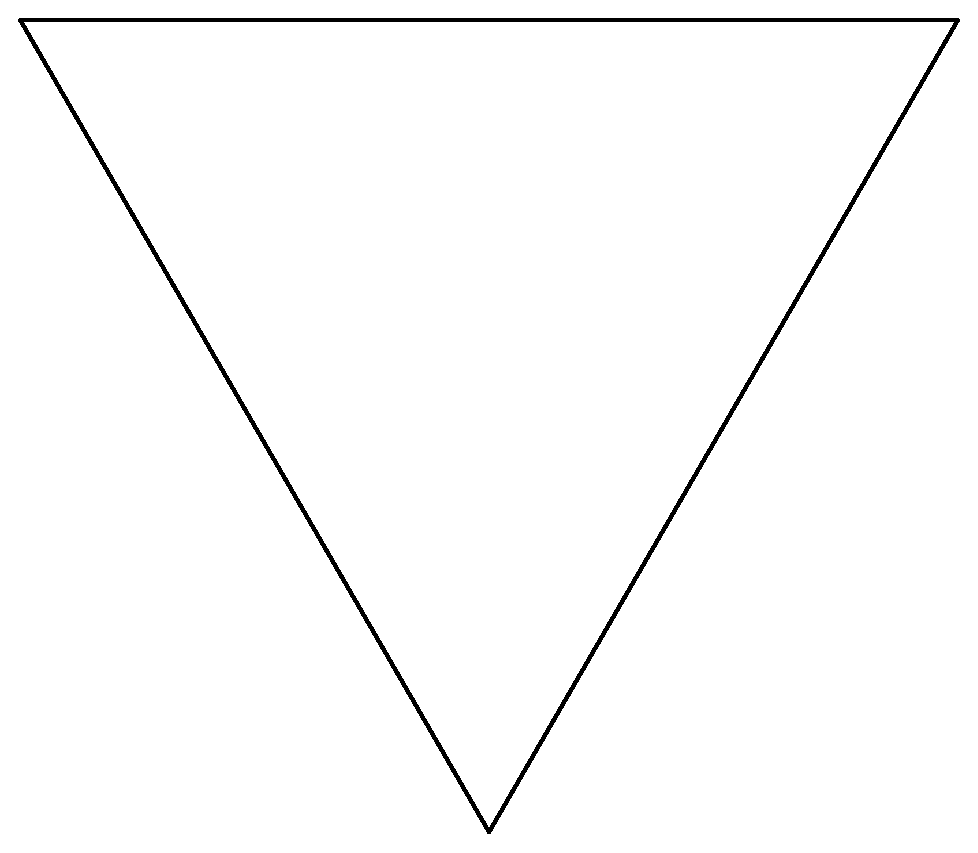
\includegraphics[scale=\fractalscale]{ch01-kochova-vlocka-0iterace.pdf}
    \end{subfigure}
    \qquad
    \begin{subfigure}{\subfigwidth}
        \centering
        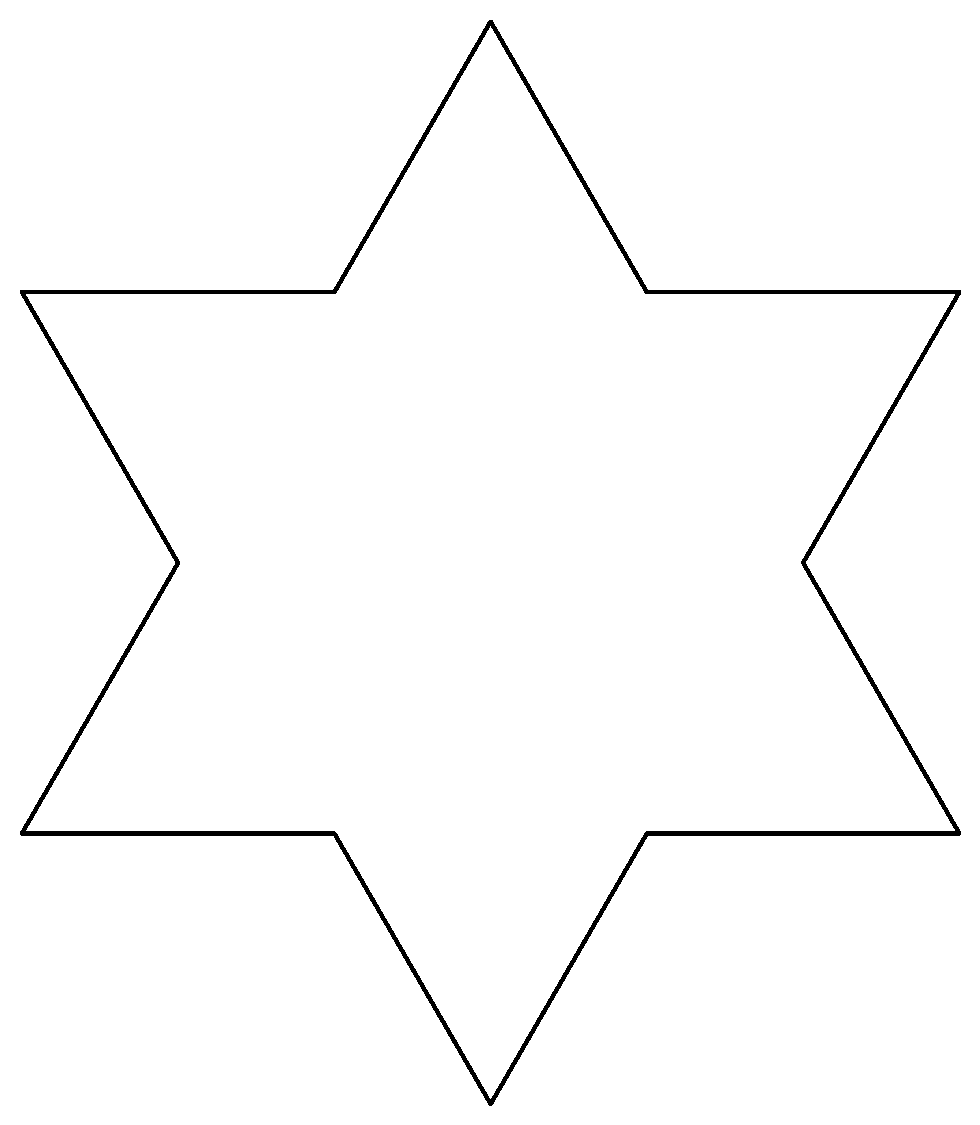
\includegraphics[scale=\fractalscale]{ch01-kochova-vlocka-1iterace.pdf}
    \end{subfigure}
    \caption{Nultá a první iterace Kochovy vločky.}
    \label{fig:kochova_vlocka_dve_iterace}
\end{figure}
\begin{figure}[h]
    \centering
    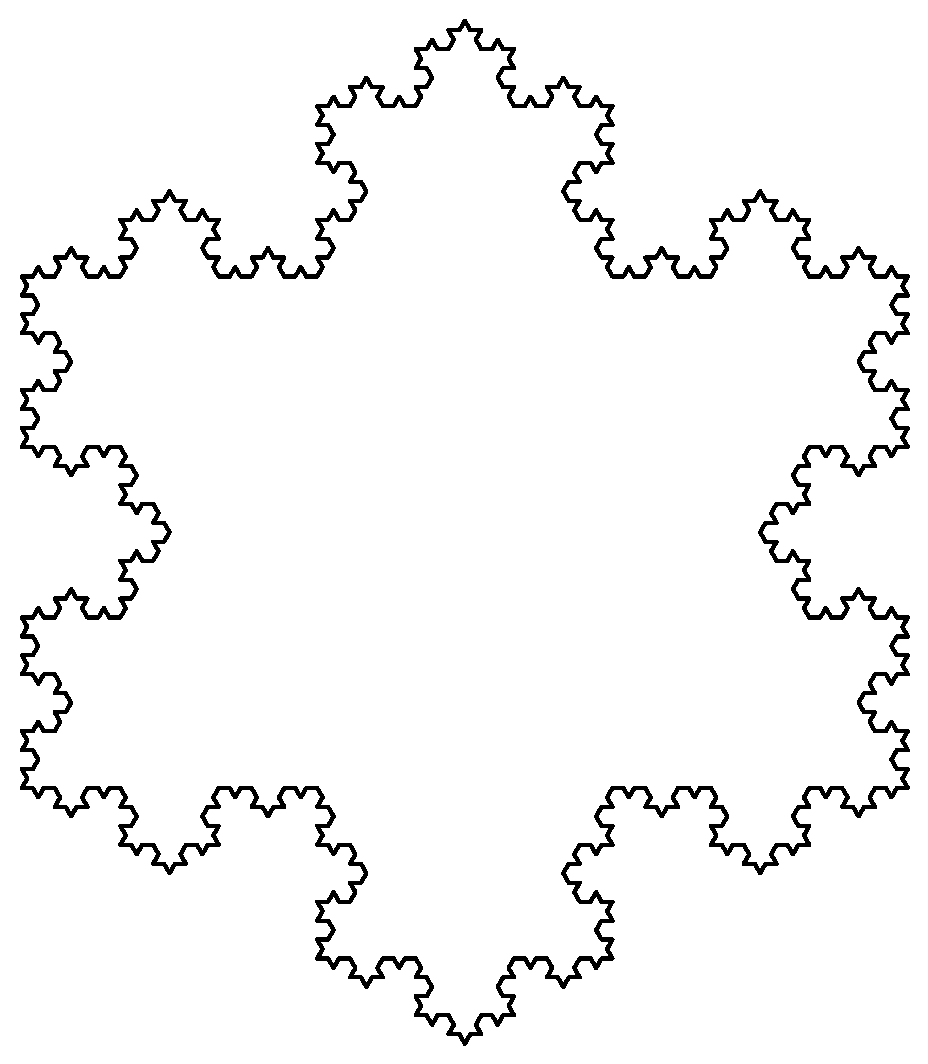
\includegraphics[scale=\fractalscale]{ch01-kochova-vlocka-4iterace.pdf}
    \caption{Čtvrtá iterace Kochovy vločky.}
    \label{fig:kochova_krivka_5iterace}
\end{figure}
Podíváme-li se na obvod,~nejspíše nás nepřekvapí,~že ten je i~zde nekonečný\footnote{Obvod Kochovy křivky po $n$-té iteraci je $o_n=3\cdot(4/3)^{n}$.} (už z~principu,~že každá strana původního rovnostranného trojúhelníka představuje samostatnou Kochovu křivku).
Obsah vzniklého útvaru je však již zajímavější. Pro zjednodušení výpočtu si rozdělme útvar na \emph{stejné rovnostranné trojúhelníky} podle obrázku \ref{fig:kochova_vlocka_rozdeleni},~jejichž obsah je roven $1/12$ obsahu obrazce v~nulté iteraci.
\begin{figure}[h]
    \centering
    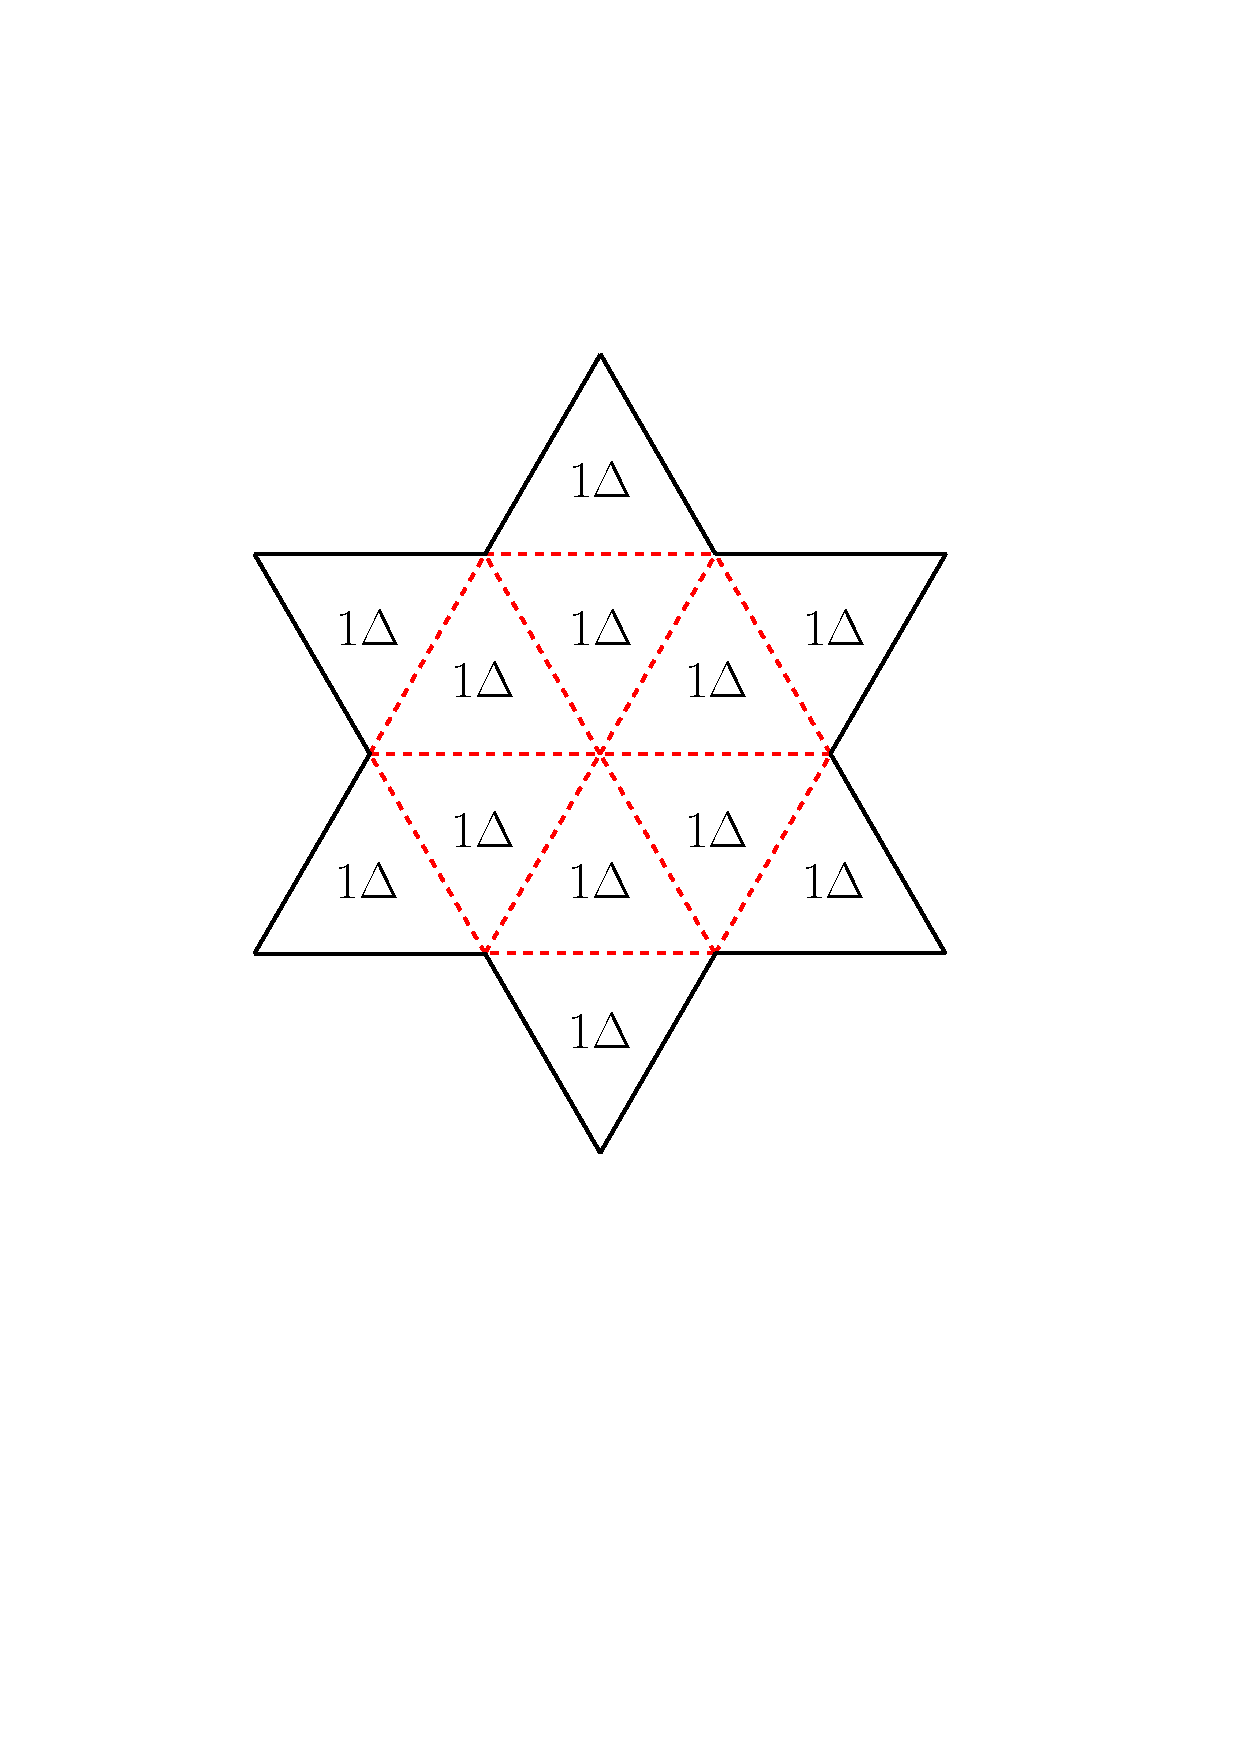
\includegraphics[scale=.4]{ch01-kochova-vlocka-rozdeleni.pdf}
    \caption{Rozdělení první iterace Kochovy vločky.}
    \label{fig:kochova_vlocka_rozdeleni}
\end{figure}
Výsledný obsah se tedy pokusíme vyjádřit relativně vůči \emph{obsahům daných trojúhelníků},~na něž jsme obrazec rozdělili,~a pak jej pouze přepočítáme. Jejich obsah si označme $\Delta$. Tedy obsah Sierpińského trojúhelníku v~nulté iteraci lze vyjádřit jako $S_0=9\Delta$. Po první iteraci vzniknou na každé ze strany 3 nové trojúhelníky o~obsahu $1/9\cdot\Delta$. V~každé další iteraci vzniknou z~jedné úsečky 4 nové. Obecně po $n$ iteracích jich tedy bude $3\cdot 4^{n}$. (Při výpočtu musíme počítat s~o jedna nižší mocninou,~neboť trojúhelníky vznikají "na úsečkách" z~předešlé iterace,~nikoliv té aktuální.)\par
Zaměřme se nyní pouze trojúhelníky,~které vznikly v~aktuální iteraci (viz obrázek \ref{fig:kochova_vlocka_2iterace_nove_trojuhelniky}). Součet jejich obsahů nám dává \emph{přírůstek obsahu} v~obecné $n$-té iteraci. Označíme-li tento přírůstek $B_n$,~pak platí
\[B_n=\underbrace{3\cdot 4^{n-1}}_{\text{počet úseček}}\cdot\overbrace{\left(\dfrac{1}{9}\right)^{n-1}\Delta}^{\text{obsah nových troj.}}=3\cdot\left(\dfrac{4}{9}\right)^{n-1}\Delta,\]
kde $n\geqslant 1$.
\begin{figure}[h]
    \centering
    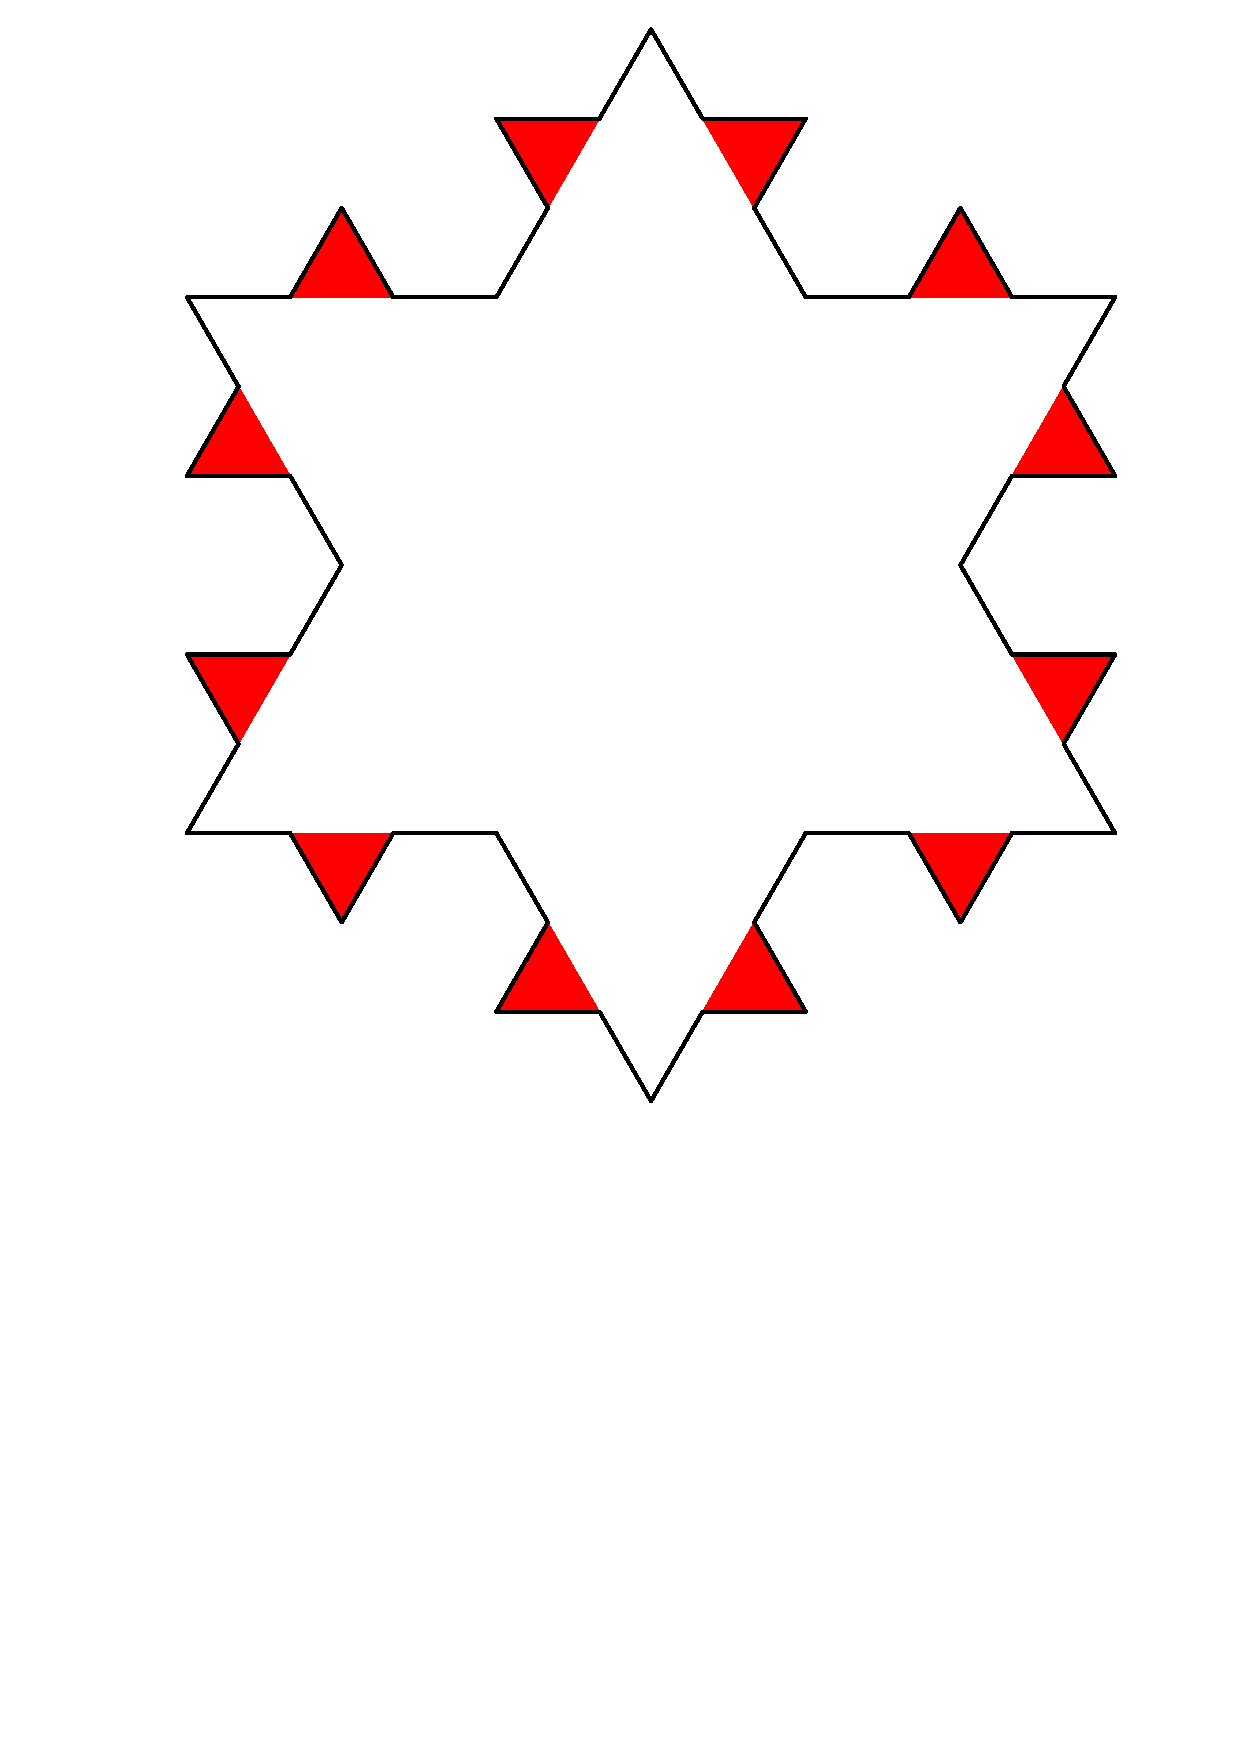
\includegraphics[scale=\fractalscale]{ch01-kochova-vlocka-2iterace-nove-trojuhelniky.pdf}
    \caption{Nově vzniklé trojúhelníky v~druhé iteraci.}
    \label{fig:kochova_vlocka_2iterace_nove_trojuhelniky}
\end{figure}
Nyní můžeme již vyšetřit obsah v~$n$-té iteraci $S_n$ a posléze i~celkový obsah výsledného obrazce $S=\lim_{n\to\infty}{S_n}$. Pro $n\geqslant 1$ platí
\begin{align*}
    S_n&=S_0+\sum_{k=1}^{n}{B_k}=9\Delta+3\Delta\cdot\sum_{k=1}^{n}{\left(\dfrac{4}{9}\right)^{k-1}}=9\Delta+3\Delta\cdot\dfrac{1-\left(\dfrac{4}{9}\right)^{n}}{1-\dfrac{4}{9}}\\
    &=9\Delta+\dfrac{27}{5}\Delta\cdot\left(1-\left(\dfrac{4}{9}\right)^n\right)
\end{align*}
Tedy
\begin{align*}
    S&=\lim_{n\to\infty}{S_n}=9\Delta+\dfrac{27}{5}\Delta\cdot\left(1-\left(\dfrac{4}{9}\right)^n\right)=9\Delta+\dfrac{27}{5}\Delta\cdot\left(1-\lim_{n\to\infty}\left(\dfrac{4}{9}\right)^n\right)\\
    &=9\Delta+\dfrac{27}{5}\Delta=\dfrac{72}{5}\Delta.
\end{align*}
Obsah trojúhelníků,~na než jsme rozdělili první iteraci Kochovy vločky,~je
\[\Delta=\dfrac{\sqrt{3}}{4}\cdot\dfrac{1}{9}\]
a tedy celkově
\[S=\dfrac{72}{5}\Delta=\dfrac{72}{5}\cdot\dfrac{\sqrt{3}}{4}\cdot\dfrac{1}{9}=\dfrac{2\sqrt{3}}{5}.\]
Byl to trochu delší výpočet,~nicméně jsme zjistili,~že Kochova vločka má (stejně jako Kochova křivka) \emph{nekonečnou délku (obvod)},~ale obsah má \emph{konečný}.
% Obsah vzniklého útvaru je však již zajímavější. Po první iteraci přibudou 3 nové trojúhelníky se stranou délky $1/3$,~tzn. jejich obsah bude
% \begin{equation*}
%     \dfrac{\sqrt{3}}{4}\left(\dfrac{1}{3}\right)^2
% \end{equation*}
% a celkový obsah obrazce tedy bude
% \begin{equation*}
%     S_1=\dfrac{\sqrt{3}}{4}+3\cdot\dfrac{\sqrt{3}}{4}\left(\dfrac{1}{3}\right)^2.
% \end{equation*}
% V~každé další iteraci vzniknou z~jedné úsečky 4 nové. Obecně po $n$ iteracích jich bude $3\cdot 4^n$ (při výpočtu však musíme počítat s~o jedna nižší mocninou,~neboť trojúhelníky vznikají "na úsečkách" z~předešlé iterace,~nikoliv té aktuální,~viz obrázek \ref{fig:kochova_vlocka_2iterace_nove_trojuhelniky}).
% \begin{figure}[h]
%     \centering
%     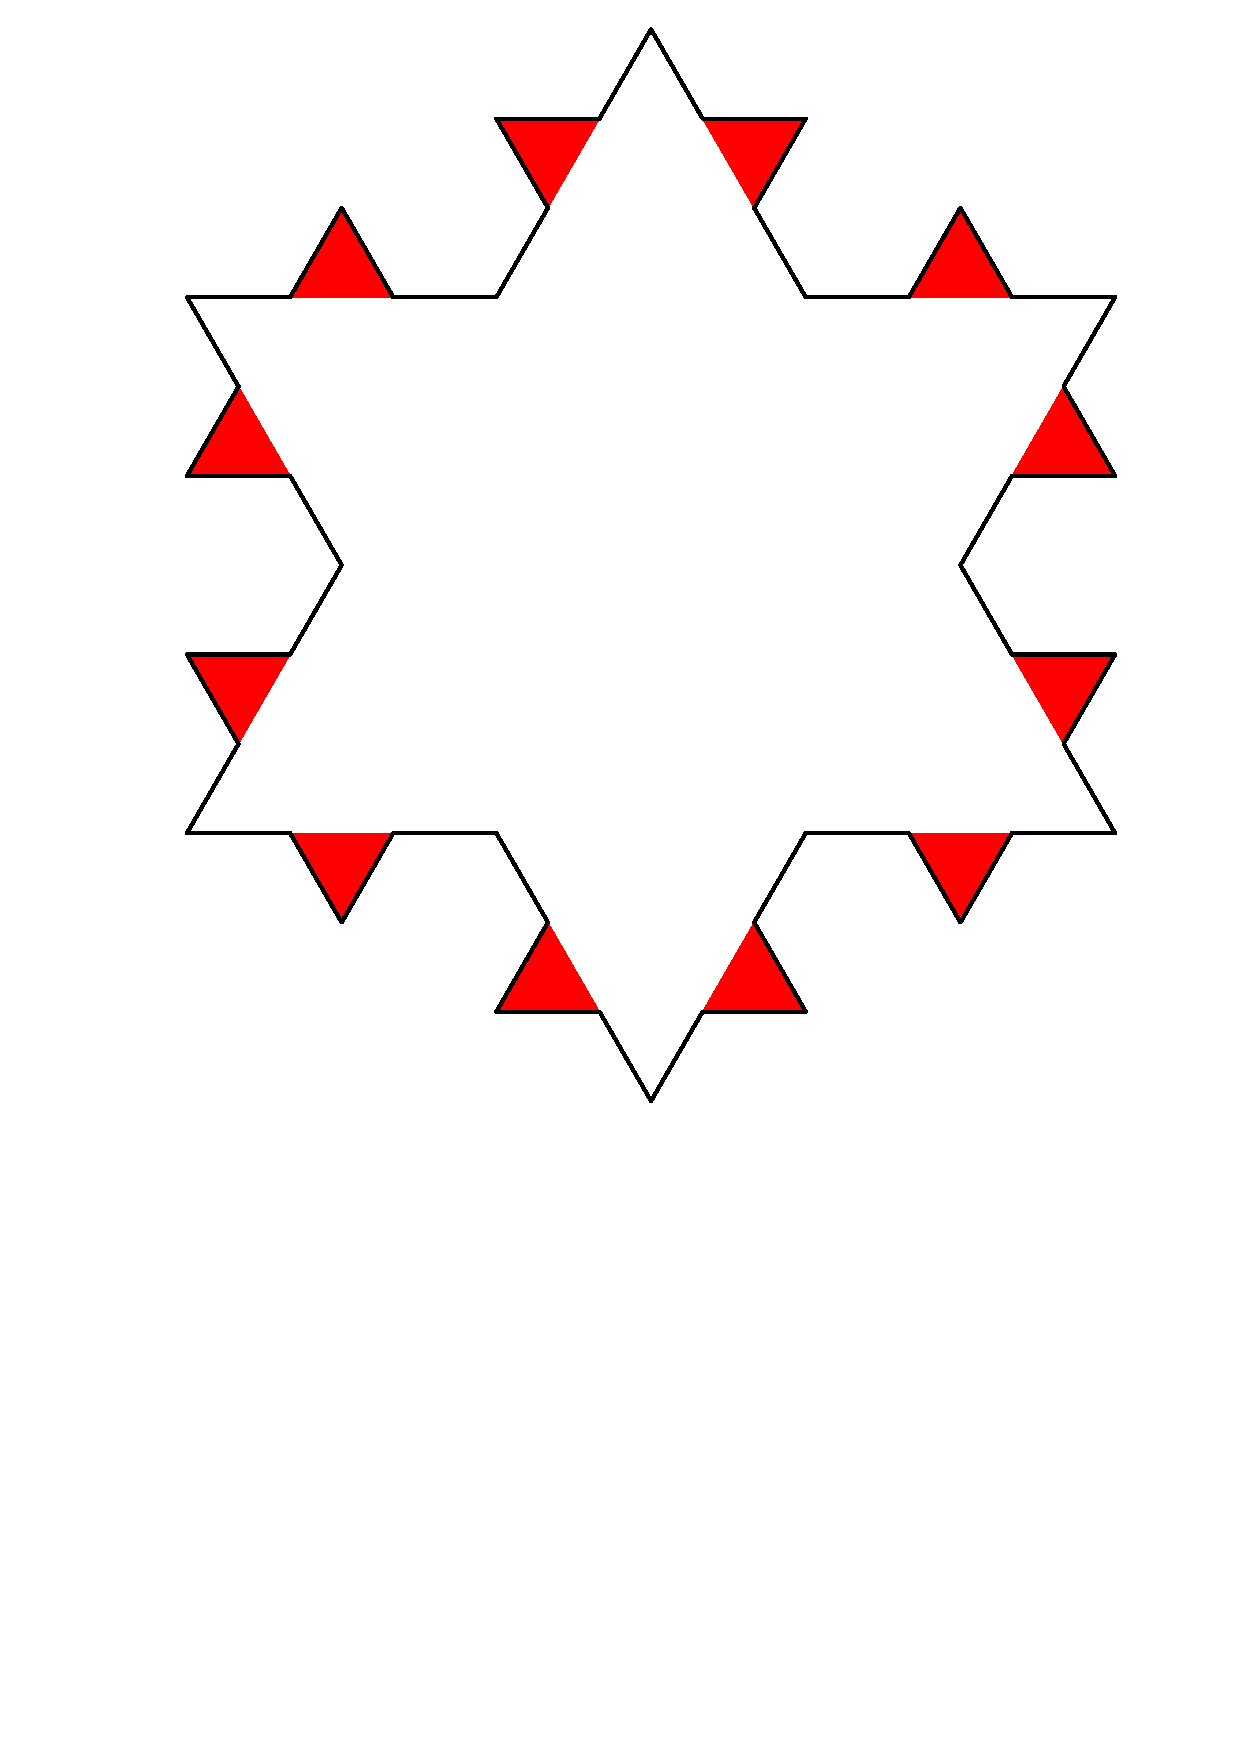
\includegraphics[scale=\fractalscale]{ch01-kochova-vlocka-2iterace-nove-trojuhelniky.pdf}
%     \caption{Nově vzniklé trojúhelníky v~druhé iteraci.}
%     \label{fig:kochova_vlocka_2iterace_nove_trojuhelniky}
% \end{figure}
% Délka úseček,~a tedy i~stran nově vzniklých rovnostranných trojúhelníků,~je $(1/3)^n$. Celkový obsah nově vzniklých trojúhelníků je tak
% \begin{equation}\label{eq:obsah_novych_trojuhelniku}
%     3\cdot 4^{n-1}\cdot\dfrac{\sqrt{3}}{4}\left(\dfrac{1}{3^n}\right)^2.
% \end{equation}
% Pro další výpočet bude pro nás výhodné si výraz \eqref{eq:obsah_novych_trojuhelniku} upravit.
% \begin{equation*}
%     3\cdot 4^{n-1}\cdot\dfrac{\sqrt{3}}{4}\left(\dfrac{1}{3^n}\right)^2=\dfrac{3\sqrt{3}}{4^2}\cdot \dfrac{4^n}{3^{2n}}=\dfrac{3\sqrt{3}}{16}\left(\dfrac{4}{9}\right)^n.
% \end{equation*}
% Celkový obsah obrazce po $n$ iteracích lze tak vypočítat součtem obsahů všech vzniklých trojúhelníků ve všech předešlých iteracích,~tj.
% \begin{equation*}
%     S_n=\sum_{k=1}^n{S_k}=\overbrace{\dfrac{\sqrt{3}}{4}}^{S_0}+\sum_{k=1}^n{\dfrac{3\sqrt{3}}{16}\left(\dfrac{4}{9}\right)^k}.
% \end{equation*}
% Suma na pravé straně představuje geometrickou řadu s~kvocientem $4/9$. Úpravou získáme
% \begin{equation}\label{eq:kochova_vlocka_obsah_n_iteraci}
%     \dfrac{\sqrt{3}}{4}+\dfrac{3\sqrt{3}}{16}\sum_{k=1}^n{\left(\dfrac{4}{9}\right)^k}=\dfrac{\sqrt{3}}{4}+\dfrac{3\sqrt{3}}{16}\cdot\dfrac{4}{9}\cdot\dfrac{1-\left(\dfrac{4}{9}\right)^n}{1-\dfrac{4}{9}}=\dfrac{\sqrt{3}}{4}+\dfrac{3\sqrt{3}}{20}\left(1-\left(\dfrac{4}{9}\right)^n\right)
% \end{equation}
% Můžeme si všimnout,~že výraz \eqref{eq:kochova_vlocka_obsah_n_iteraci} bude tentokrát již konečné číslo,~neboť limitním přechodem pro $n\to\infty$ se výraz $(4/9)^n$ bude blížit nule. Celkově tedy máme
% \begin{align*}
%     S&=\lim_{n\to\infty}S_n=\lim_{n\to\infty}\left(\dfrac{\sqrt{3}}{4}+\dfrac{3\sqrt{3}}{20}\left(1-\left(\dfrac{4}{9}\right)^n\right)\right)=\dfrac{\sqrt{3}}{4}+\dfrac{3\sqrt{3}}{20}\left(1-\lim_{n\to\infty}\left(\dfrac{4}{9}\right)^n\right)\\
%     &=\dfrac{\sqrt{3}}{4}+\dfrac{3\sqrt{3}}{20}=\dfrac{2\sqrt{3}}{5}.
% \end{align*}

\subsection{Cantorovo diskontinuum}\label{subsec:cantorovo_diskontinuum}
Podívejme se ještě na jeden typ fraktálního objektu,~kterým je tzv. \emph{Cantorovo diskontinuum}\footnote{Též se mu říká \emph{Cantorova množina} (angl. \emph{"Cantor set"})\index{Cantorovo diskontinuum}\index{diskontinuum!Cantorovo}. Dvourozměrnou variantou je pak tzv. \emph{Cantorův prach}\index{Cantorův prach}\index{prach!Cantorův} (angl. \emph{"Cantor dust"}). Slovo \emph{prach} je zde míněno v~přeneseném významu,~neboť (podobně jako v~této podsekci) lze ukázat,~že vzniklé útvary mají v~limitě nulový obsah.} Myšlenka je zde velmi jednoduchá: začínáme s~úsečkou délky $1$ (nultá iterace) a následně odebereme prostřední třetinu,~čímž vznikne první iterace. V~dalších iteracích postupujeme analogicky pro vzniklé úsečky (viz obrázek \ref{fig:cantorovo_diskontinuum}).
\begin{figure}[h]
    \centering
    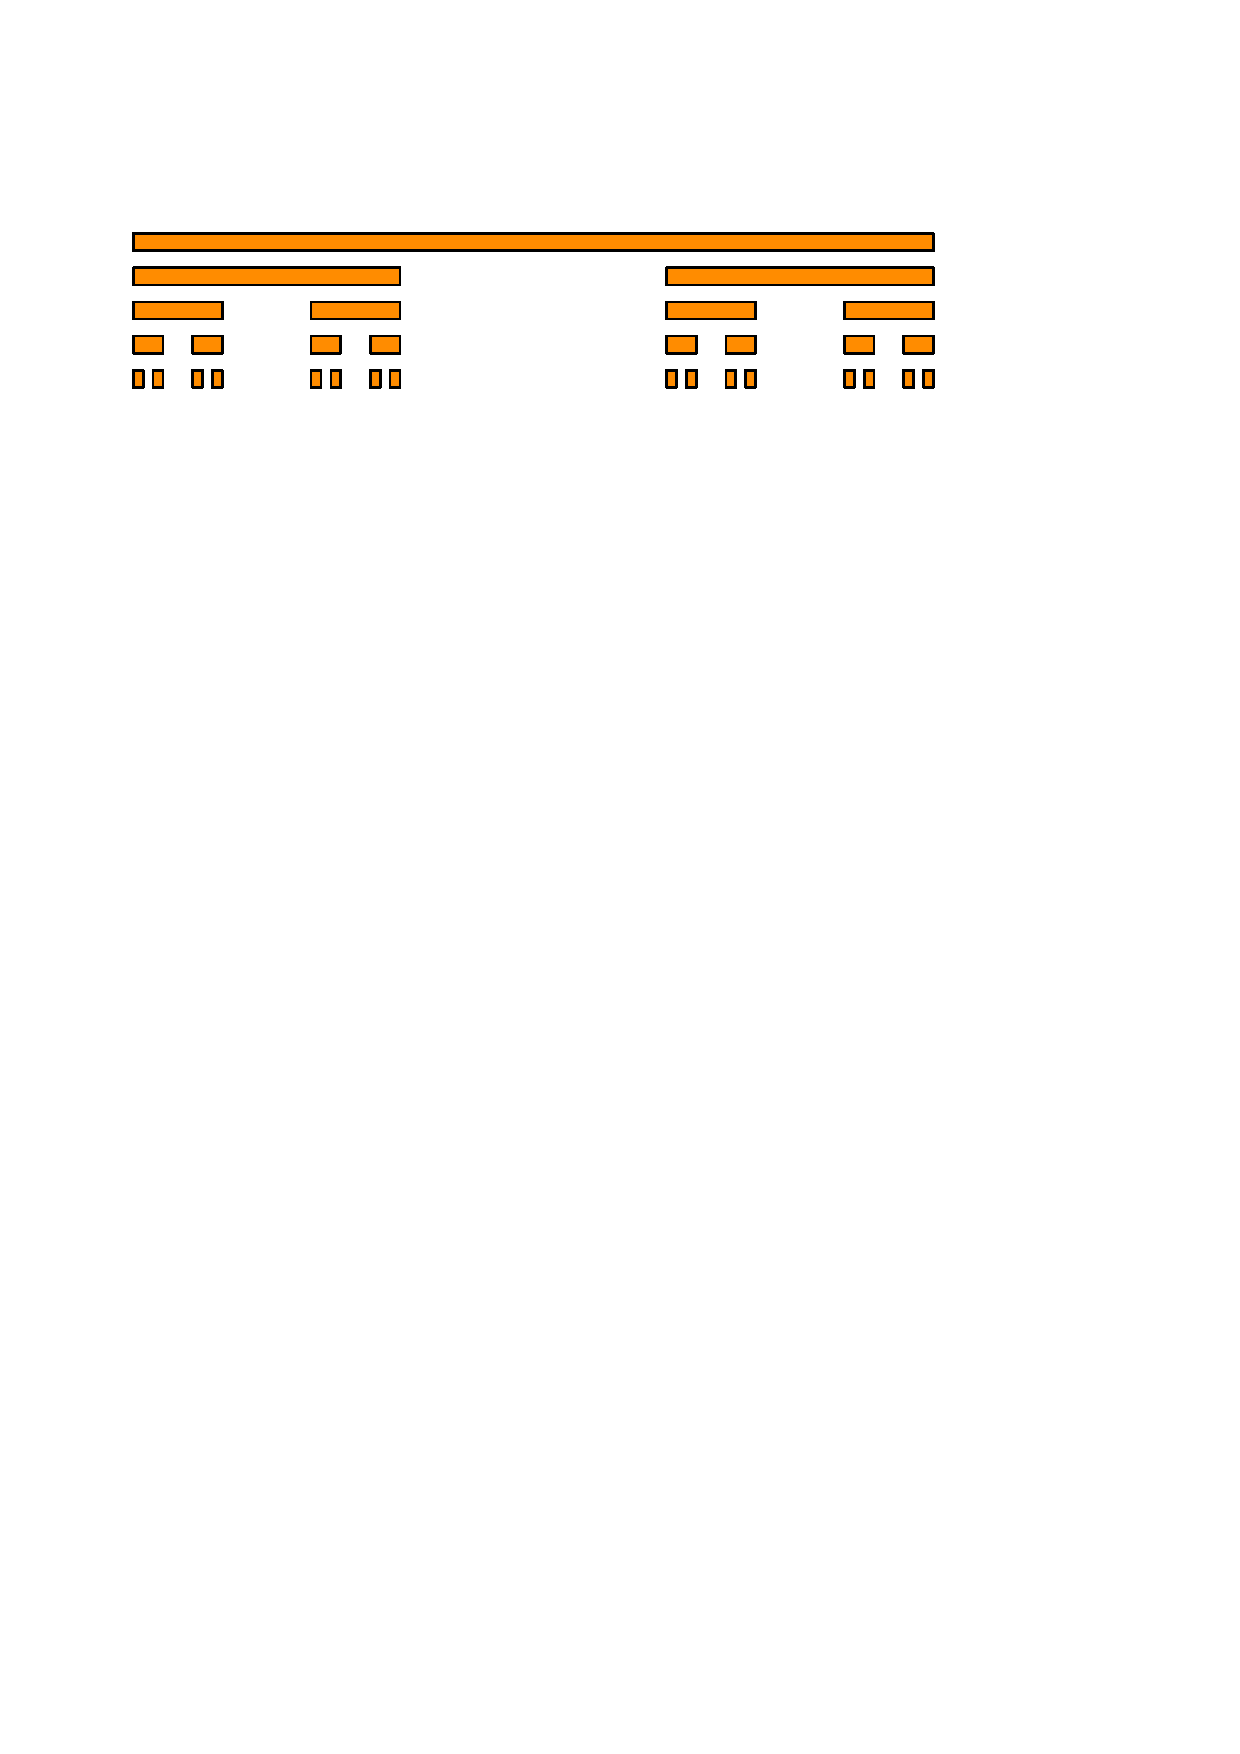
\includegraphics[scale=\normalipe]{ch01-cantorova-mnozina.pdf}
    \caption{Nultá až čtvrtá iterace Cantorova diskontinua.}
    \label{fig:cantorovo_diskontinuum}
\end{figure}

Nově vzniklé úsečky třetinové délky jsou kopiemi původní úsečky. Stejně jako u~předešlých fraktálů nás i~zde bude zajímat limitní chování tohoto procesu. Lze očekávat,~že postupným odebíráním zbudou úsečky nulové délky. O~tom se lze přesvědčit např. tak,~že spočítáme limitu celkových délek všech odebraných úseků. V~první iteraci odebereme úsečku délky $1/3$,~v~druhé iteraci odebereme dvě celkové délky $2\cdot(1/3)^2=2/9$,~ve třetí vyjmeme čtyři celkové délky $4\cdot(1/3)^3=4/27$,~atd. (viz obrázek \ref{fig:cantorovo_diskontinuum_delky}).
\begin{figure}[h]
    \centering
    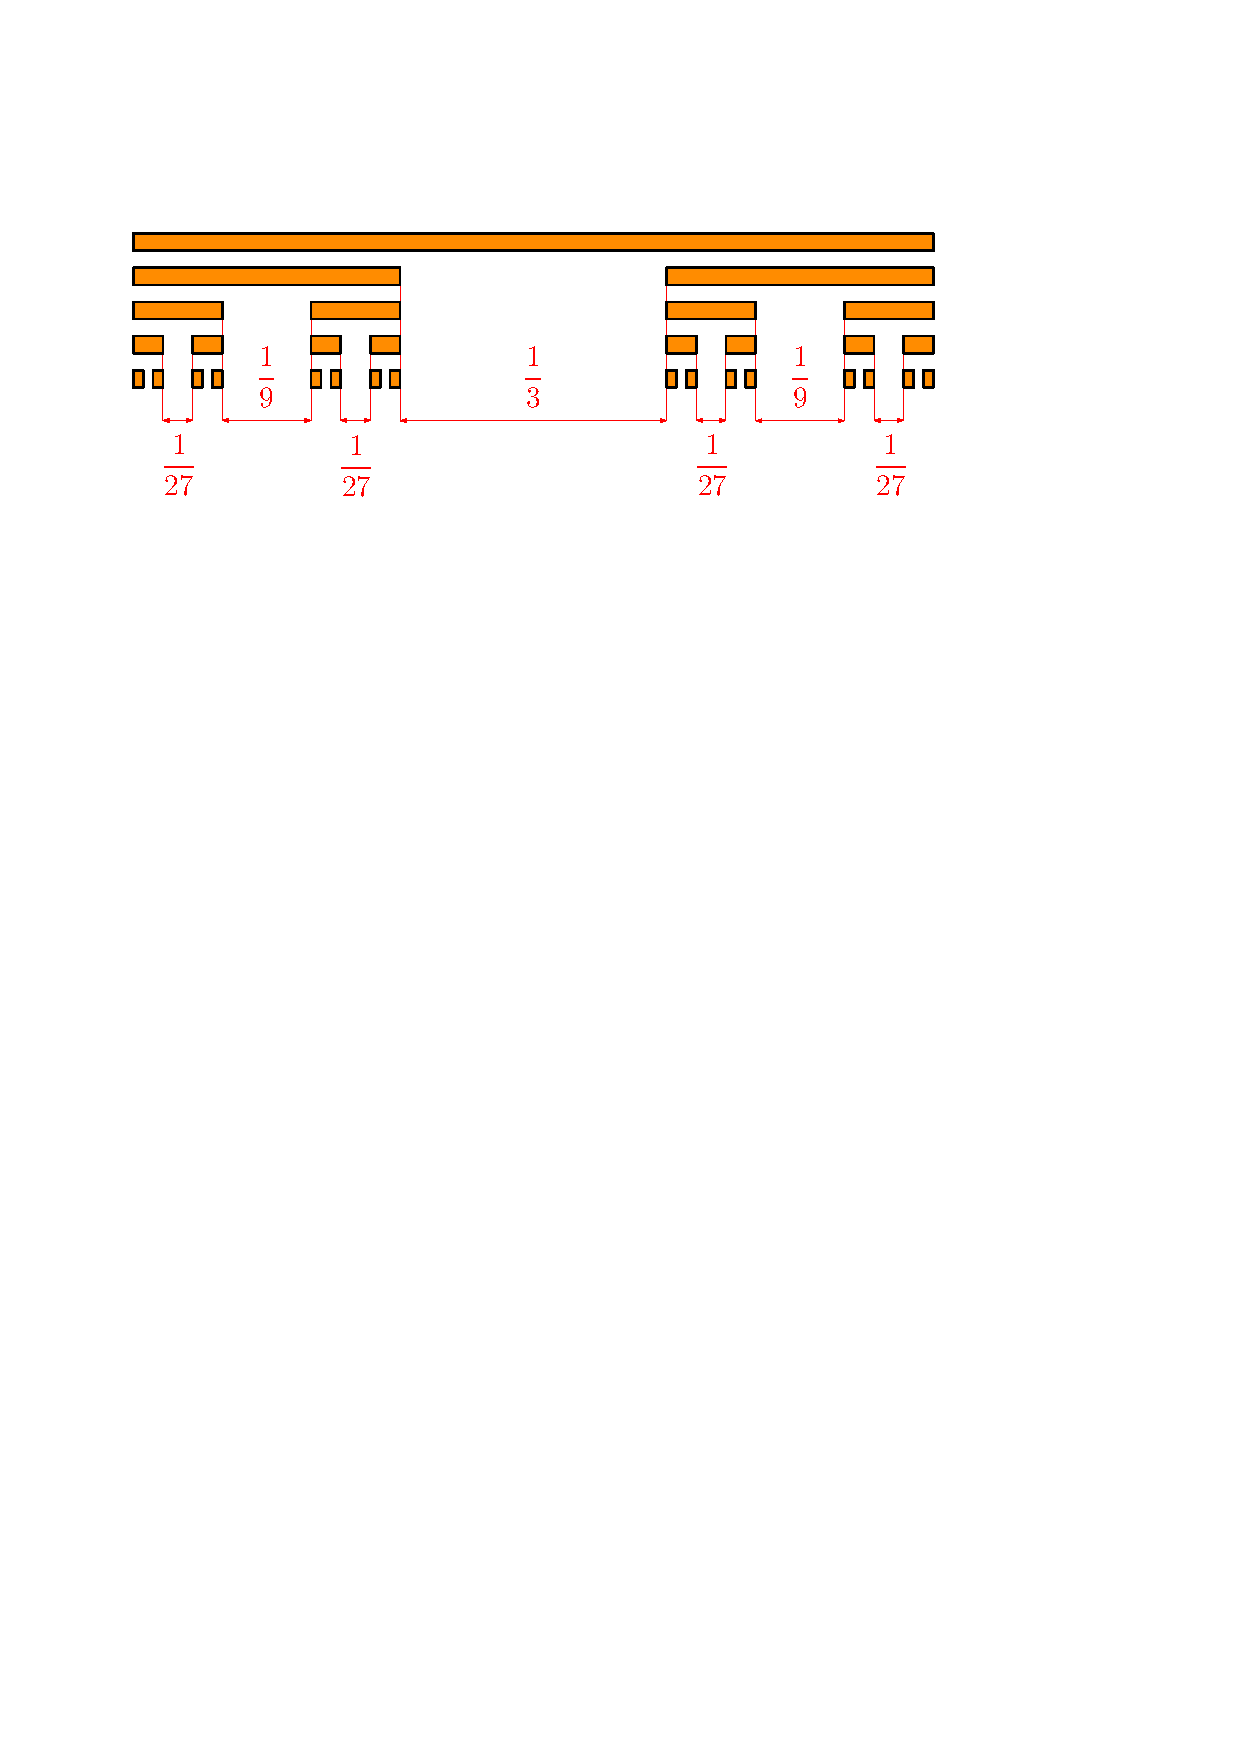
\includegraphics[scale=\normalipe]{ch01-cantorova-mnozina-delky.pdf}
    \caption{Znázornění délek vyjmutých úseků.}
    \label{fig:cantorovo_diskontinuum_delky}
\end{figure}
Obecně počet odebraných úseků roste s~mocninou dvojky,~jejichž délky klesají s~mocninou trojky,~tedy v~$n$-té iteraci odebereme úsek délky $2^n(1/3)^{n+1}$. Označíme-li tedy délku zbylých úseků $\ell_n$ po $n$ iteracích a $\overline{\ell_n}$ délku odebraných úseků,~pak určitě platí $\ell_n=1-\overline{\ell_n}$. Protože nás zajímá délka \emph{všech} odebraných úseků,~pak po $n$ iteracích bude celková délka rovna
\begin{equation}
    \overline{\ell_n}=\sum_{k=0}^{n}2^k\left(\dfrac{1}{3}\right)^{k+1}=\sum_{k=0}^{n}\dfrac{2^k}{3^{k+1}}=\dfrac{1}{3}\cdot\sum_{k=0}^{n}\left(\dfrac{2}{3}\right)^k=\dfrac{1}{3}\cdot\dfrac{1-\left(\dfrac{2}{3}\right)^{n+1}}{1-\dfrac{2}{3}}=1-\left(\dfrac{2}{3}\right)^{n+1}.
\end{equation}
Označíme-li si limitu výrazů posloupností $\ell_n$,~reps. $\overline{\ell_n}$,~jako $\ell$,~resp. $\overline{\ell}$,~pak dostaneme
\begin{equation*}
    \overline{\ell}=\lim_{n\to\infty}\overline{\ell_n}=\lim_{n\to\infty}\left(1-\left(\dfrac{2}{3}\right)^{n+1}\right)=1-\lim_{n\to\infty}\left(\dfrac{2}{3}\right)^{n+1}=1-0=1.
\end{equation*}
Z toho již triviálně plyne,~že
\begin{equation}
    \ell=\lim_{n\to\infty}\ell_n=\lim_{n\to\infty}(1-\overline{\ell_n})=1-\lim_{n\to\infty}\overline{\ell_n}=1-1=0,
\end{equation}
tzn. na konci procesu zbude Cantorovo diskontinuum délky nula.
\section{Fraktální dimenze}\label{sec:fraktalni_dimenze}

\subsection{Chápání konceptu dimenze}\label{subsec:koncept-dimenze}

Útvary vyčtené v~sekci~\ref{sec:sobepodobnost} ilustrují vlastnost soběpodobnosti,~kterou jsme si (zatím neformálně) popsali. V~eukleidovské geometrii lze však u~mnohých základních objektů pozorovat stejnou vlastnost. Např. čtverec lze určitě prohlásit v~jistém smyslu za soběpodobný,~neboť jej lze rozdělit na podobné útvary (viz obrázek~\ref{fig:sobepodobnost-ctverce}).
\begin{figure}[h]
    \centering
    \begin{subfigure}[b]{\subfigwidth}
        \centering
        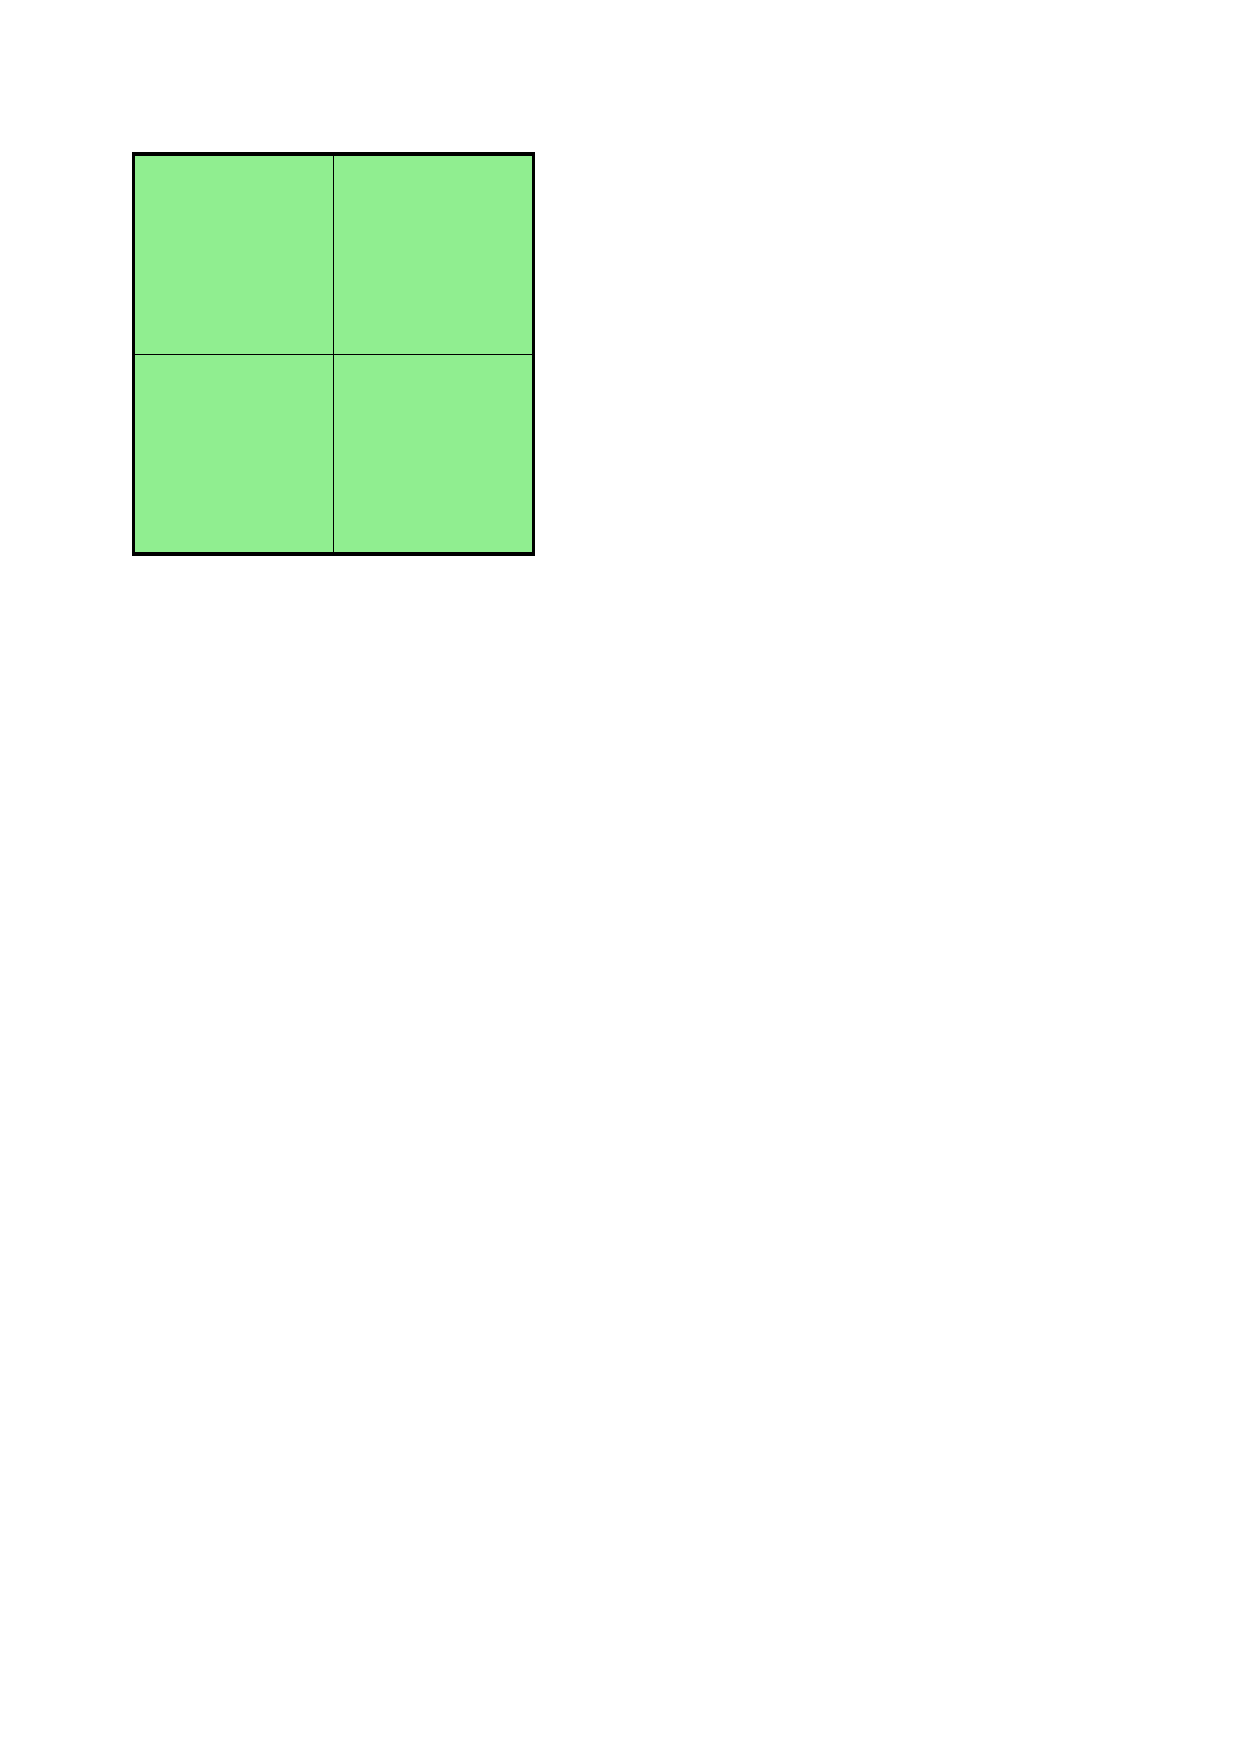
\includegraphics[scale=\normalipe]{ch01-ctverec-sobepodobnost.pdf}
        \caption{Rozdělení na čtyři menší čtverce.}
        \label{subfig:sobepodobnost-ctverce-1}
    \end{subfigure}
    \begin{subfigure}[b]{\subfigwidth}
        \centering
        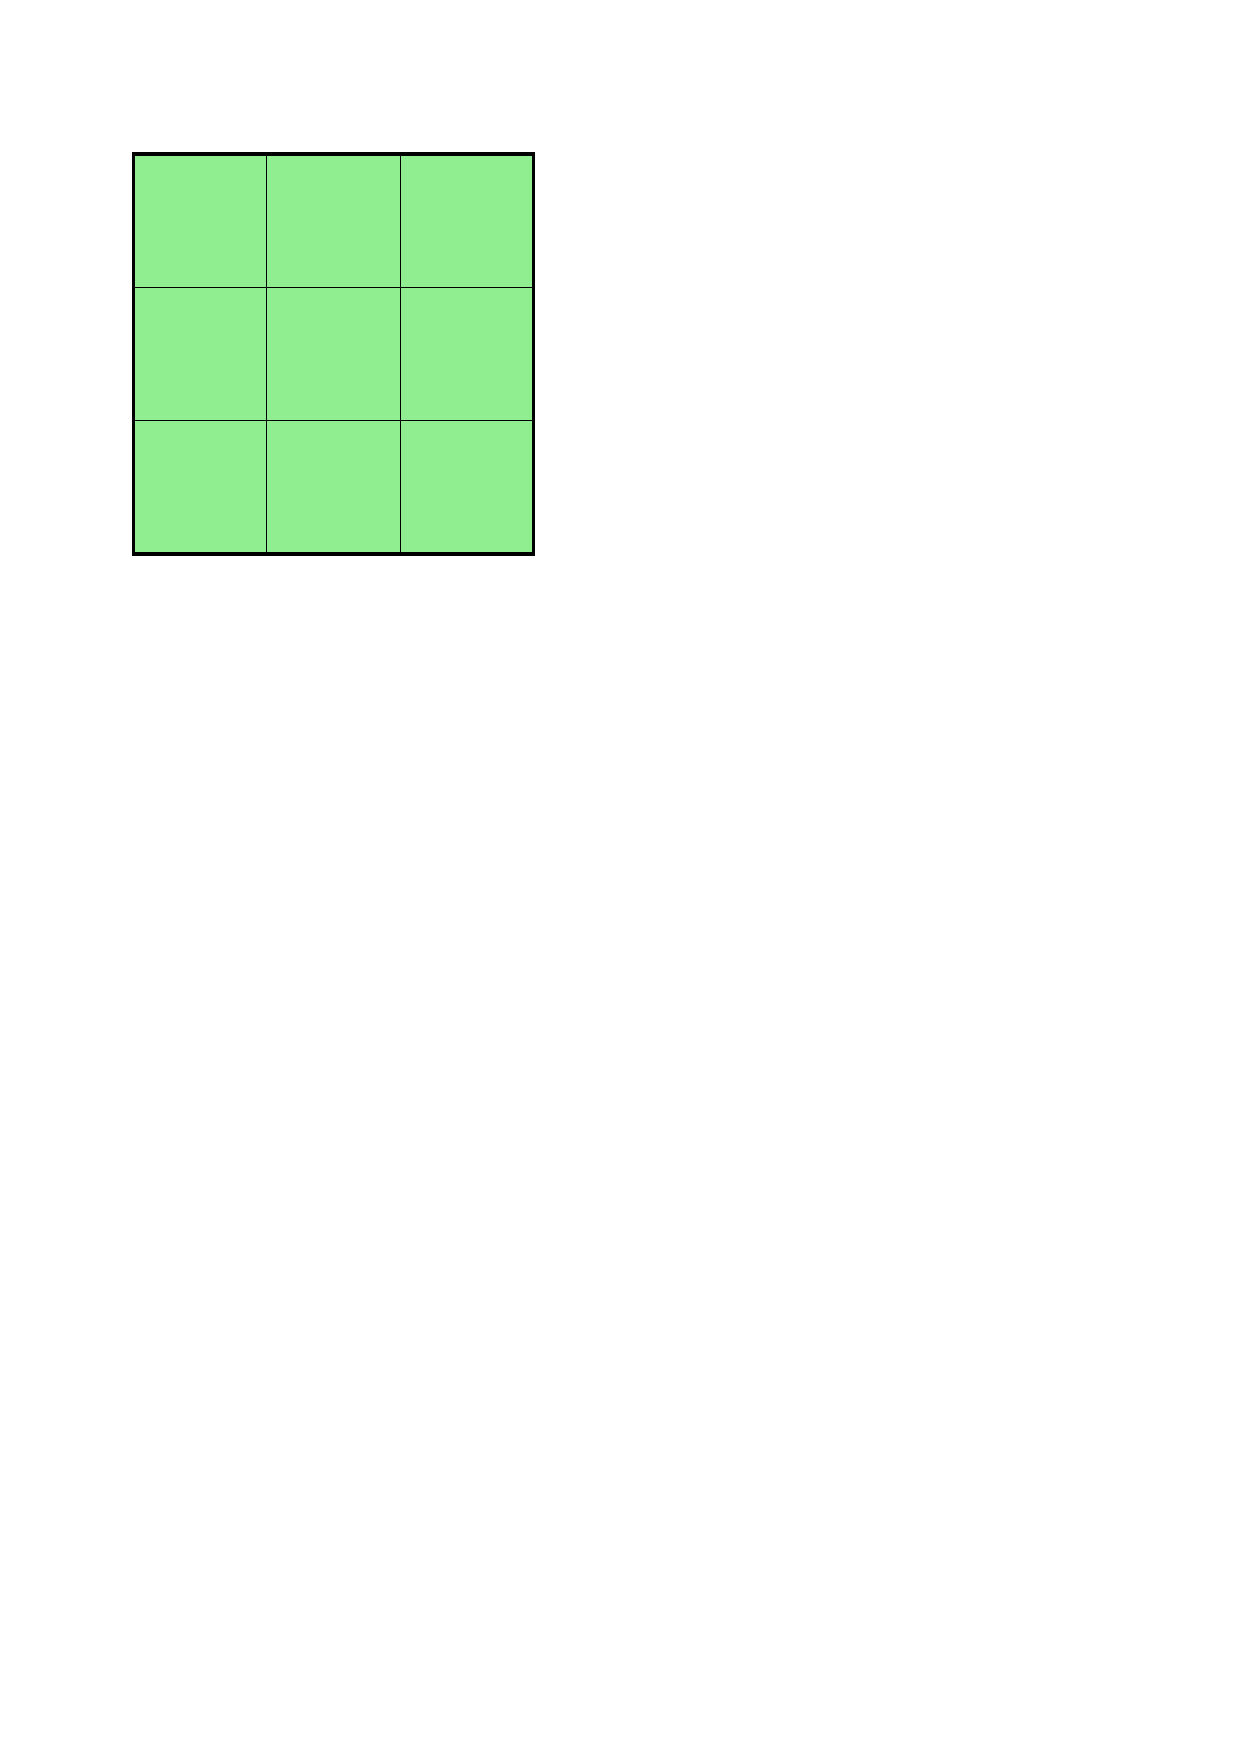
\includegraphics[scale=\normalipe]{ch01-ctverec-sobepodobnost-2.pdf}
        \caption{Jiná možnost rozdělení čtverce.}
        \label{subfig:sobepodobnost-ctverce-2}
    \end{subfigure}
    \caption{Soběpodobnost čtverce.}
    \label{fig:sobepodobnost-ctverce}
\end{figure}
Podobně např. i~obyčejná úsečka je taktéž soběpodobná,~protože ji můžeme rozdělit na $k$ stejných částí (viz obrázek~\ref*{fig:sobepodobnost-usecky}).\par
\begin{figure}[h]
    \centering
    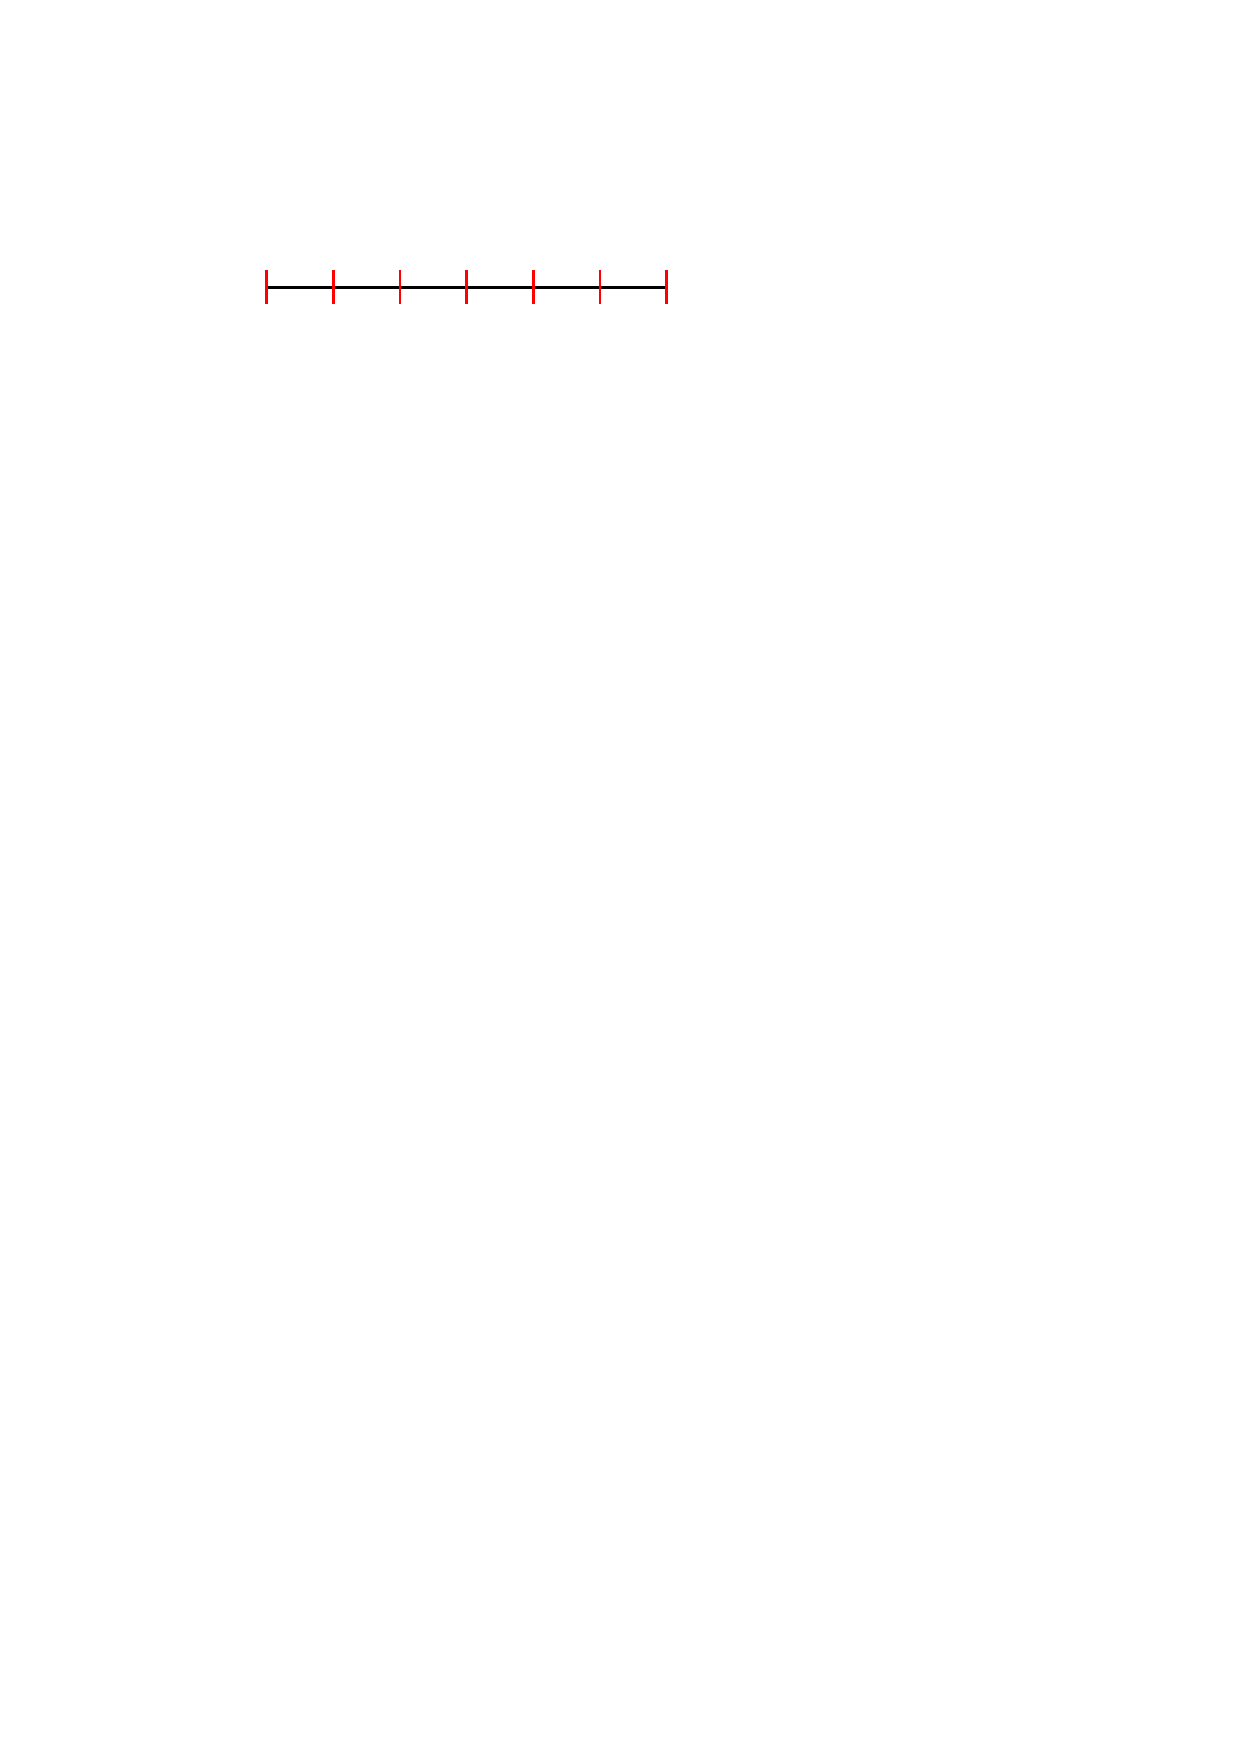
\includegraphics[scale=\normalipe]{ch01-usecka-sobepodobnost.pdf}
    \caption{Úsečka rozdělená na šest stejných částí.}
    \label{fig:sobepodobnost-usecky}
\end{figure}
K čemu nám takové uvědomění vlastně je? Zmenšíme-li úsečku $k$-krát,~pak budeme potřebovat přesně $k$ těchto částí,~abychom dostali úsečku původní délky. U~čtverce (nebo obdélníku obecně) při změnšení délky strany $k$-krát budeme potřebovat $k^2$ daných útvarů pro obdržení čtverce s~původním obsahem.\footnote{Obdélník zmenšený $k$-krát bude mít strany délek $a/k,\,b/k$,~tedy jeho obsah bude
\[\dfrac{ab}{k^2}=\dfrac{S}{k^2},\]
kde $S$ je obsah původního obdélníka.}
Pro krychli bude situace podobná,~$k$-krát zmenšená kopie bude potřeba $k^3$-krát,~abychom dostali krychli o~původním objemu (viz obrázek~\ref{fig:krychle-sobepodobnost}).
\begin{figure}[h]
    \centering
    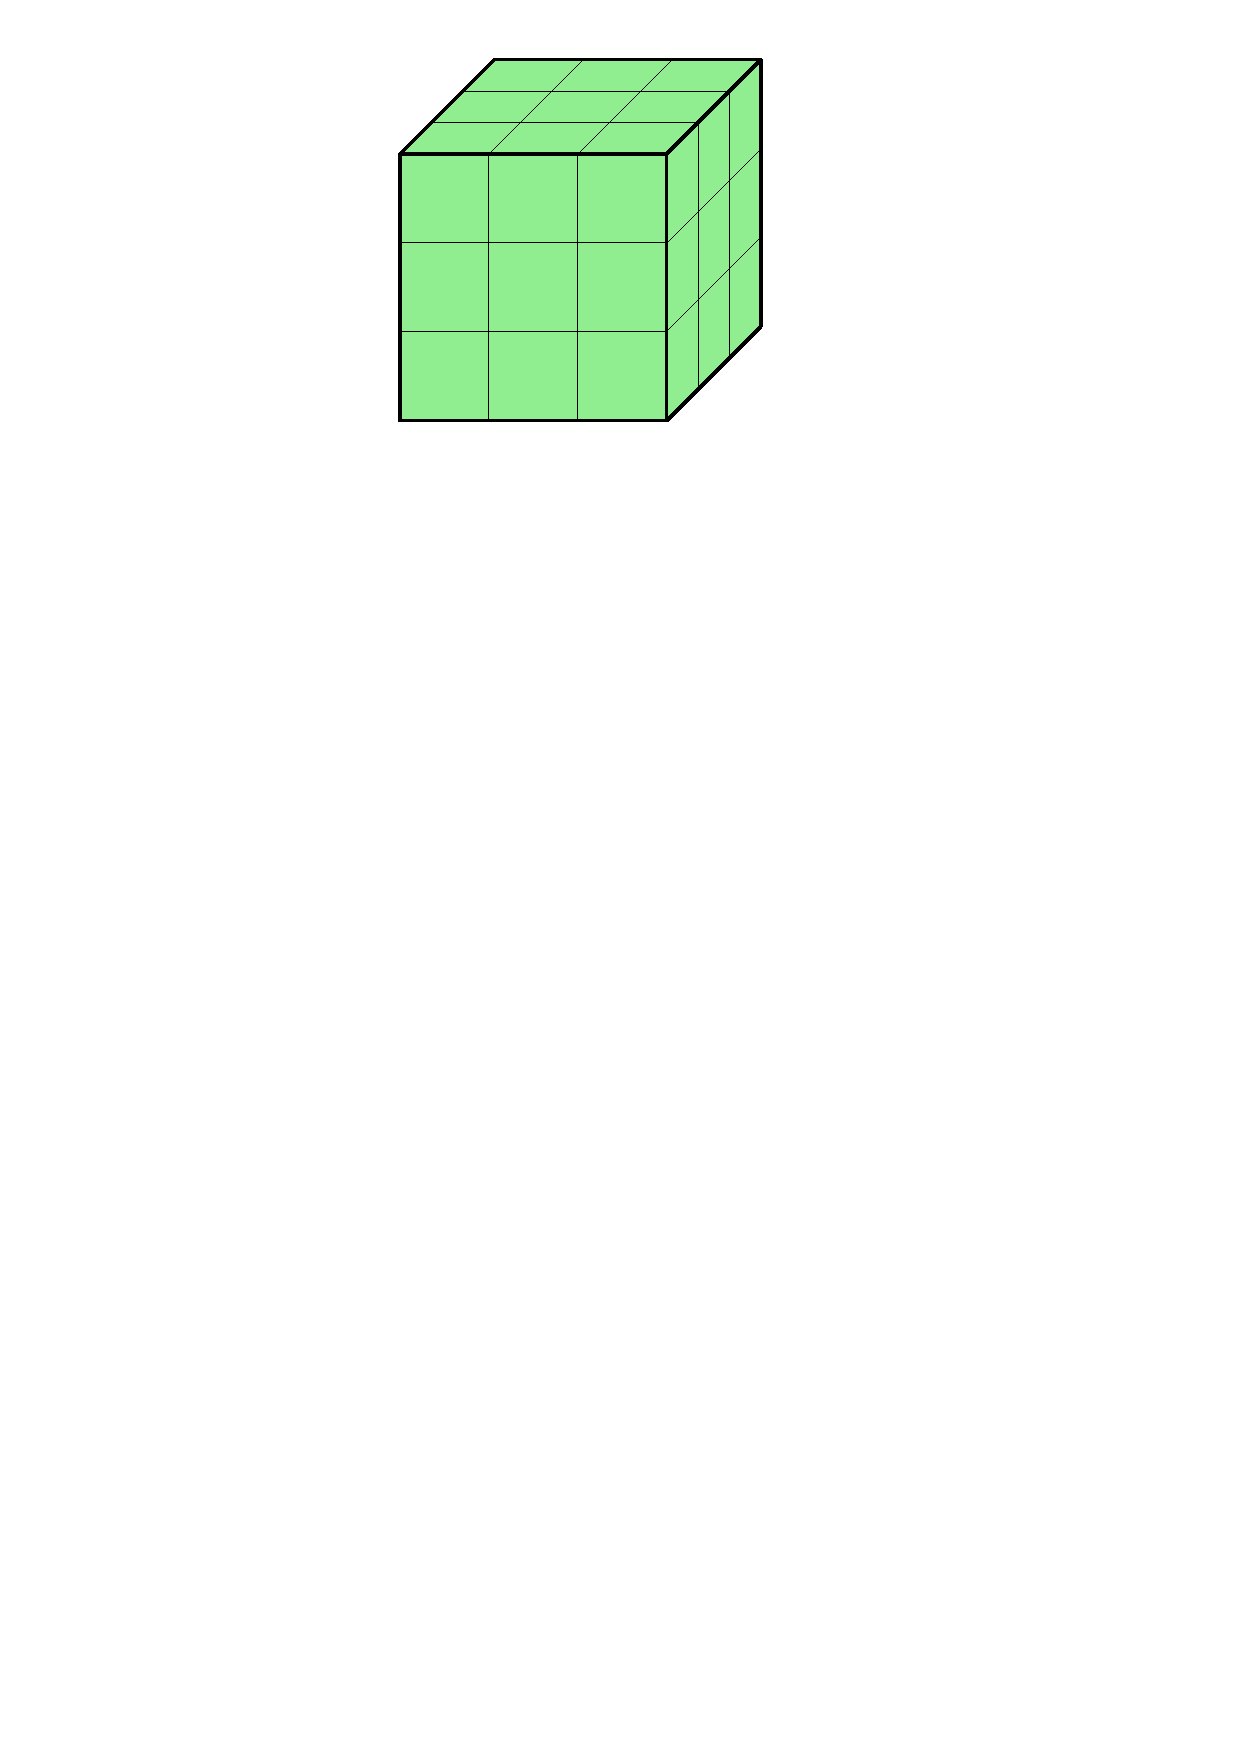
\includegraphics[scale=\normalipe]{ch01-krychle-sobepodobnost.pdf}
    \caption{Krychle rozdělená na 27 stejných částí.}
    \label{fig:krychle-sobepodobnost}
\end{figure}
Lze si všimnout,~že v~závislosti na \emph{dimenzi} objektu se mění daný exponent. Vztah lze tak zobecnit na
\begin{equation}\label{eq:pocet-utvaru}
    N(k)=k^d
\end{equation}
kde $N(k)$ je počet nových útvarů v~závislosti na faktoru $k$ a~číslu $d$. Intuitivně je nejspíše jasné,~že dimenze útvaru je takové číslo $d$,~pro které platí rovnost \eqref{eq:pocet-utvaru}.

Toto je jeden z~možných způsobů,~jak lze chápat koncept dimenze. Jednoduchou úpravou rovnosti \eqref{eq:pocet-utvaru} dostaneme
\[d=\log_k{N(k)}=\dfrac{\ln{N(k)}}{\ln{k}}.\]
(Obecně lze volit jakýkoliv přípustný základ logaritmů,~tj $d=\log_b{N(k)}/\log_b{k}$ pro $b\in\R_+\setminus\set{1}$.)

Dimenze v~tomto pojetí skutečně dává dobrý smysl. Pro "klasické" geometrické objekty vychází dimenze vždy celočíselně (viz tabulka \ref{table:eukleides-dimenze}).
\begin{table}[h]
    \centering
    \begin{tabular}{r|cc}
    Útvar    & $N(k)$ & $d=\ln{N(k)}/\ln{k}$ \\ \hline
    Úsečka   & $3$      & $1$                          \\
    Čtverec  & $9$      & $2$                          \\
    Krychle  & $27$     & $3$                          \\
    Teserakt & $81$     & $4$                          \\
    \end{tabular}
    \caption{Hodnoty dimenze $d$ pro různé útvary.}
    \label{table:eukleides-dimenze}
\end{table}

Na této myšlence je založen pojem tzv. \emph{fraktální dimenze}\index{fraktální dimenze}\index{dimenze!fraktální}. Existuje více neekvivalentních způsobů její definice. Jedna z~nich,~které se dále nyní v~této sekci budeme držet,~se v~anglicky psané literatuře nazývá \emph{"box-counting dimension"}\index{box-counting dimenze}\index{dimenze!box-counting},~odkud plyne i~značení $\dimB$. Pro útvar $F$ (formálně vzato množinu bodů) definujeme 
\begin{equation}\label{eq:fraktalni-dimenze}
    \dimB{F}=\lim_{\varepsilon\to 0_+}{\dfrac{\ln{N_\varepsilon(F)}}{\ln{\left(\frac{1}{\varepsilon}\right)}}}.
\end{equation}
(Převzato z~\cite[str. 93]{Zelinka2006} a~\cite[str. 28]{Falconer2014}.) Výraz $1/\varepsilon$ zde představuje faktor podobnosti jako původní $k$ (samotné $\varepsilon$ tak hraje roli měřítka). Číslo $N_\varepsilon(F)$ je počet soběpodobných útvarů,~na které jsme rozdělili původní útvar $F$ v měřítku $\varepsilon$. Největší rozdíl zde však představuje zkoumání "limitního chování" daného výrazu.

Nejdříve poznamenejme, pro "klasické" geometrické útvary hodnota $\dimB{F}$ vychází skutečně tak, jak jsme zvyklí. Toto si ilustrujeme na příkladech~\ref{ex:fraktalni-dimenze-usecka},~\ref{ex:fraktalni-dimenze-ctverec} a~\ref{ex:fraktalni-dimenze-trojuhelnik}.
\begin{example}[Fraktální dimenze úsečky]\label{ex:fraktalni-dimenze-usecka}
    Začněme asi nejednodušším příkladem výpočtu fraktální dimenze,~a to u~úsečky (označme $\ell$). Představme si,~že úsečku \emph{jednotkové délky} rozdělíme na $N_\varepsilon(\ell)=n$ shodných dílů. Pak měřítko libovolného dílu je
    \[\varepsilon=\dfrac{1}{n}=n^{-1}.\]
    (Zde je dobré si uvědomit,~že pro $n\to\infty$,~tedy zjemňování dělení úsečky,~platí,~že $\varepsilon\to 0_+$.) Fraktální dimenzi úsečky vypočteme z~definice jako
    \[\dimB{\ell}=\lim_{\varepsilon\to 0_+}{\dfrac{\ln{N_\varepsilon(\ell)}}{\ln{\left(\frac{1}{\varepsilon}\right)}}}=\lim_{n\to\infty}{\dfrac{\ln{n}}{\ln{n}}}=1.\]
\end{example}
\begin{example}[Fraktální dimenze čtverce]\label{ex:fraktalni-dimenze-ctverec}
    Podobně,~jako v~příkladu~\ref{ex:fraktalni-dimenze-usecka}\linebreak{}výše,~můžeme stanovit i~fraktální dimenzi čtverce (označme $S$). Uvažujme tedy čtverec o~jednotkovém obsahu,~který rozdělíme $N_\varepsilon(S)=n$ shodných útvarů. Přitom víme,~že obsah mění kvadraticky vůči délce strany. Měřítko nového čtverce tak bude
    \[\varepsilon=\sqrt{\dfrac{1}{n}}=n^{-1/2}\]
    a~fraktální dimenze vychází
    \[\dimB{S}=\lim_{n\to\infty}{\dfrac{\ln{n}}{\ln{n^{1/2}}}}=\lim_{n\to\infty}{\dfrac{\ln{n}}{\frac{1}{2}\ln{n}}}=2.\]
\end{example}
Pro krychli bude výpočet naprosto analogický (viz příklad~\ref{ex:fraktalni-dimenze-ctverec}). Obecně pro $d$-rozměrnou krychli bude její fraktální dimenze\footnote{Obdobnou úvahou dojmeme k~měřítku $\varepsilon=n^{-1/d}$.} rovna $d$.\par
Zkusme se nyní oprostit od krychle k~trochu jinému útvaru.
\begin{example}[Fraktální dimenze trojúhelníka]\label{ex:fraktalni-dimenze-trojuhelnik}
    Podívejme se,~jak to dopadne s~fraktální dimenzí \emph{obecného trojúhelníku}. Každý trojúhelník $T$ lze rozdělit na čtveřici \emph{vzájemně shodných trojúhelníků $T_1,\dots,T_4$},~které vzniknou sestrojením středních příček v~původním trojúhelníka (viz obrázek~\ref{fig:trojuhelnik-sobepodobnost}).
    \begin{figure}[h]
        \centering
        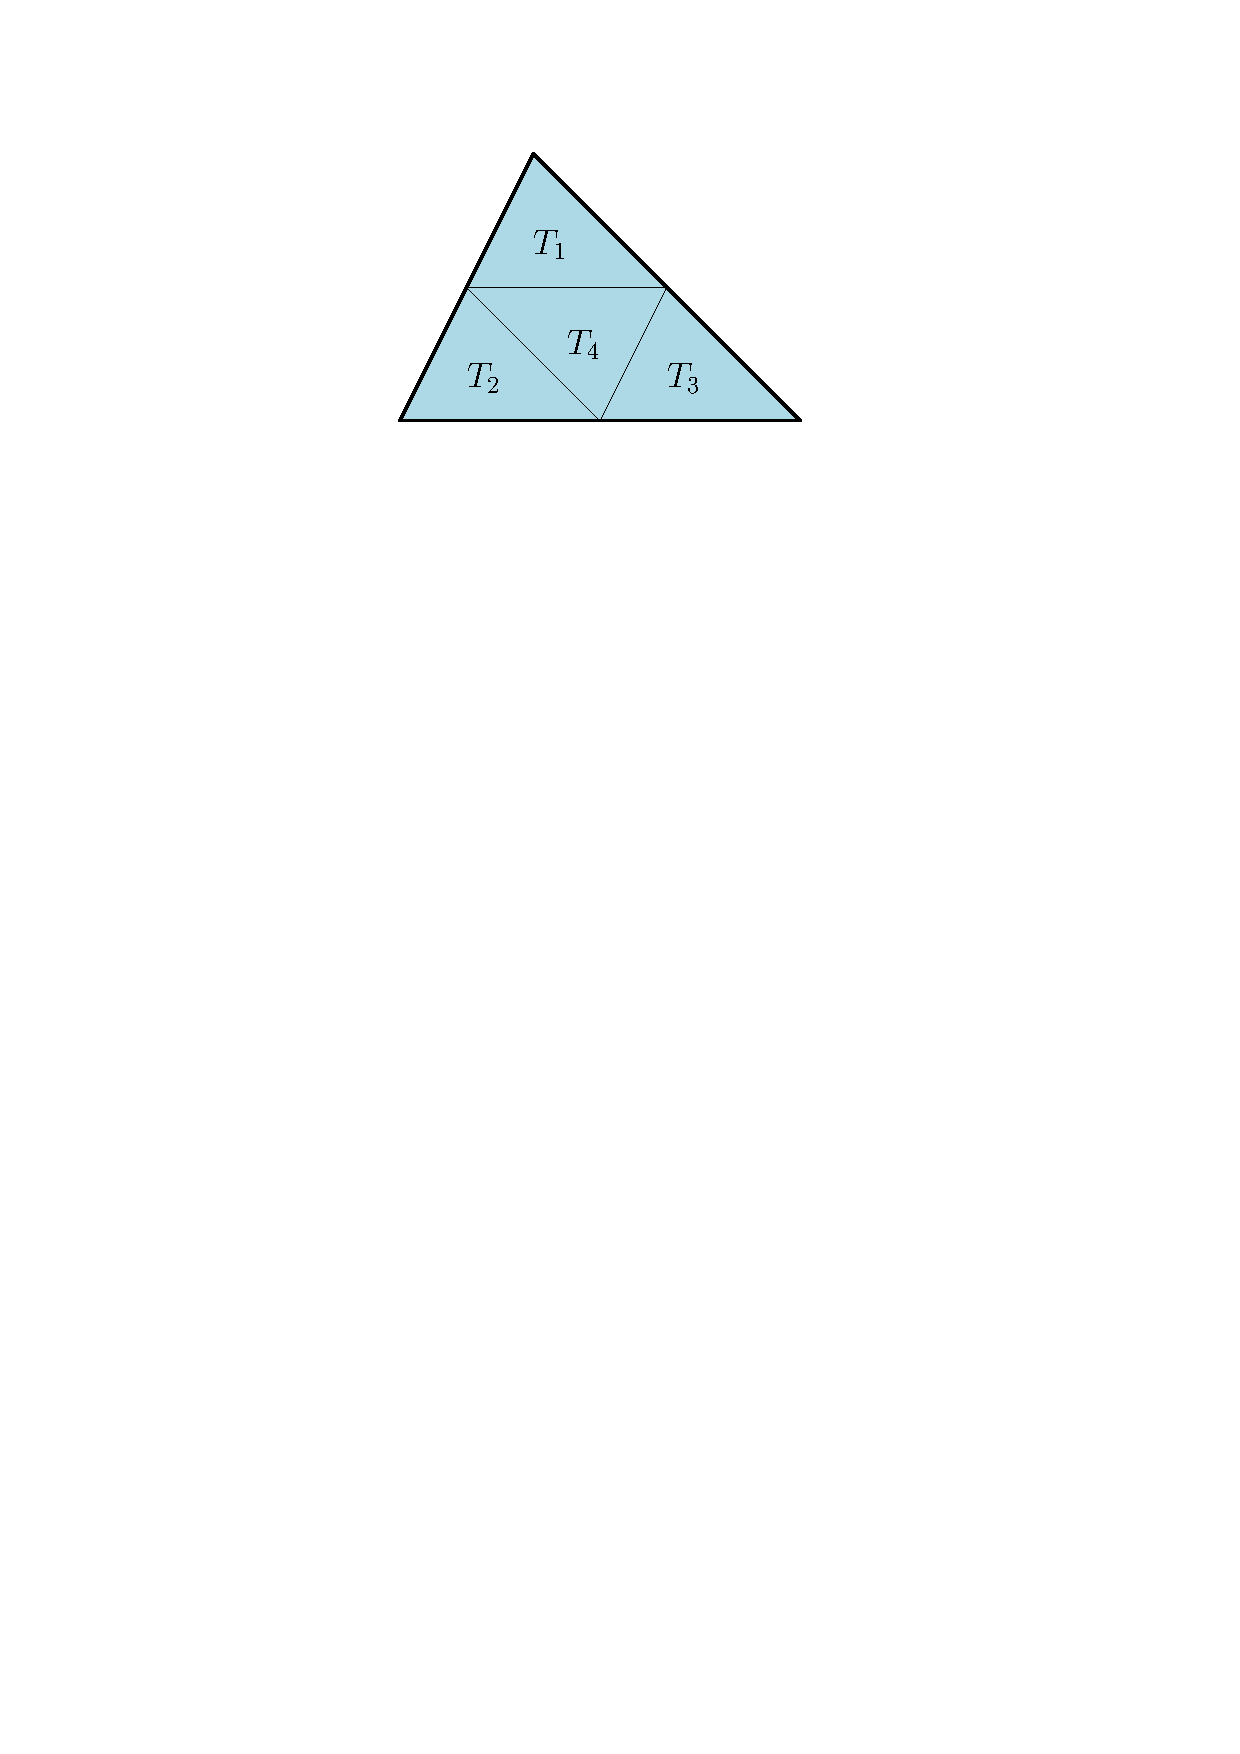
\includegraphics[scale=\normalipe]{ch01-trojuhelnik-sobepodobnost.pdf}
        \caption{Trojúhelník $T$ rozdělený na trojúhelníky $T_1,\dots,T_4$.}
        \label{fig:trojuhelnik-sobepodobnost}
    \end{figure}
    Délka každé střední příčky odpovídá polovině délky strany,~s~níž je rovnoběžná,~tedy obsah každého z~menších trojúhelníků je \emph{čtvrtina obsahu původního} trojúhelníka $T$. Tento postup můžeme opakovat pro každý z menších trojúhelníků, čímž dostaneme $4^2$ trojúhelníků. Takto můžeme postupovat libovolně dlouho,~přičemž po $n$ krocích bude počet\footnote{Výpočet bychom mohli i~zde provést ve stejném duchu jako u~úsečky,~čtverce nebo krychle. Počet částí,~na než rozdělíme trojúhelník,~označíme $N_\varepsilon(T)=n$,~přičemž měřítko pak bude $\varepsilon=n^{-1/2}$.} vzniklých trojúhelníků $N_\varepsilon(T)=4^n$,~přičemž měřítko každého z~nich bude $\varepsilon=(1/2)^n$. Fraktální dimenze tak vychází:
    \[\dimB{T}=\lim_{n\to\infty}{\dfrac{\ln{4^n}}{\ln{2^n}}}=\lim_{n\to\infty}{\dfrac{2n\ln{2}}{n\ln{2}}}=2.\]
\end{example}
Pro jednoduché útvary vychází dimenze tak,~jak bychom mohli očekávat. K~zajímavějším výsledkům však dospějeme u~fraktálů,~na něž se blíže podíváme v~následující podsekci~\ref{subsec:dimenze-fraktalu}.

\subsection{Dimenze fraktálů}\label{subsec:dimenze-fraktalu}

Co kdybychom však zkusili podobnou myšlenku aplikovat i~na \emph{fraktální objekty} jako např. Kochovu křivku, Kochovu vločku, Sierpińského trojúhelník nebo Cantorovo diskontinuum? Zkusme to. Pro připomenutí jednotlivých křivek a~výsledků k~nim si dovoluji čtenáře opětovně odkázat na sekci~\ref{sec:sobepodobnost},~kde jsou podrobněji rozebrány.

V tomto případě uvidíme,~že dochází na první pohled k~docela zvláštnímu jevu. Fraktální dimenze již totiž nemusí vycházet celočíselně,~jak jsme zvyklí.
\begin{itemize}
    \item \textbf{Kochova křivka $F_{KC}$.} V~každé iteraci nahrazujeme každou úsečku čtyřmi novými. Kompletní Kochova křivka tak obsahuje právě \emph{čtyři} kopie sebe sama zmenšené na třetinu,~tj. v~$n$-té iteraci je $N_\varepsilon(F_{KC})=4^n$,~jak jsme již odvodili (viz podsekce~\ref{subsec:kochova_krivka}).\footnote{Lze však zvolit i~jiné dělení. Např. lze na Kochovu křivku nahlížet,~že obsahuje \emph{16 kopií} sebe sama zmenšených na \emph{devítinu}.} Měřítko nově vzniklých částí je tak $\varepsilon=(1/3)^n$.
    \begin{equation}\label{eq:kochova-krivka-dimenze}
        \dimB{F_{KC}}=\lim_{\varepsilon\to 0_+}{\dfrac{\ln{N_\varepsilon(F_{KC})}}{\ln{\left(\frac{1}{\varepsilon}\right)}}}=\lim_{n\to\infty}{\dfrac{\ln{4^n}}{\ln{3^n}}}=\dfrac{\ln{4}}{\ln{3}}\approx 1{,}2618595\dots
    \end{equation}
    \item \textbf{Kochova vločka $F_{KS}$.} Začínáme s~rovnostranným trojúhelníkem o~straně délky $1$,~na jehož stranách postupně vznikne Kochova křivka. V~$n$-té iteraci je obvod Kochovy vločky $o_n$ roven $3\cdot 4^n$,~tj. i~$N_\varepsilon(F_{KS})=3\cdot 4^n$,~kde měřítko\footnote{Měřítko se ve srovnání s~Kochovou křivkou liší v~mocnině,~neboť délku nových úseků porovnáváme s~obvodem celého trojúhelníka,~nikoliv pouze délkou jedné jeho strany. Nicméně ve výpočtu bychom se mohli omezit i~jen na jednu ze stran,~výpočet by byl tak zcela identický jako u~Kochovy křivky.} nově vzniklých úseček je $\varepsilon=1/3\cdot(1/3)^n=(1/3)^{n+1}$. Není těžké se přesvědčit,~že fraktální dimenze vychází stejně,~jako u~Kochovy křivky:
    \begin{equation}\label{eq:kochova-vlocka-dimenze}
        \dimB{F_{KS}}=\lim_{n\to\infty}{\dfrac{\ln{3\cdot 4^n}}{\ln{3^{n+1}}}}=\lim_{n\to\infty}{\dfrac{\ln{4^n}\overbrace{\left(1+\frac{\ln{3}}{\ln{4^n}}\right)}^{\to 1}}{\ln{3^n}\underbrace{\left(1+\frac{\ln{3}}{\ln{3^n}}\right)}_{\to 1}}}=\dfrac{\ln{4}}{\ln{3}}
    \end{equation}
    \item \textbf{Sierpińského trojúhelník $F_{ST}$.} V~každé iteraci vynecháme prostřední trojúhelník,~čímž vznikne \emph{trojice} nových trojúhelníků s~\emph{polovičním} měřítkem. Tzn.~$N_\varepsilon(F_{ST})=3^n$ pro $\varepsilon=(1/2)^n$,~a tedy
    \begin{equation}\label{eq:sierpinskeho-trojuhelnik-dimenze}
        \dimB{F_{ST}}=\lim_{n\to\infty}{\dfrac{\ln{3^n}}{\ln{2^{n}}}}=\dfrac{\ln{3}}{\ln{2}}\approx 1{,}5849625\dots
    \end{equation}
    \item \textbf{Cantorovo diskontinuum $F_{CD}$.} Vždy vyjmeme prostřední třetinu\linebreak{}úsečky,~čímž obdržíme \emph{dvojici} úseček \emph{třetinové} délky,~tj. $N_\varepsilon(F_{CD})=2^n$ pro $\varepsilon=(1/3)^n$. Fraktální dimenze tak vychází
    \begin{equation}\label{eq:cantorovo-diskontinuum-dimenze}
        \dimB{F_{CD}}=\lim_{n\to\infty}{\dfrac{\ln{2^n}}{\ln{3^n}}}=\dfrac{\ln{2}}{\ln{3}}\approx 0{,}6309297\dots
    \end{equation}
\end{itemize}
Udělejme si nyní menší souhrn a~porovnání dosud získaných výsledků (viz tabulka~\ref{table:fraktaly-eukleides-dimenze}).
\begin{table}[h]
    \centering
    \begin{tabular}{r|ccc}
        Útvar $F$                & $\varepsilon$ & $N_\varepsilon(F)$ & $\dimB{F}$         \\ \hline
        Úsečka                   & $n^{-1}$      & $n$                & 1                  \\
        Čtverec                  & $n^{-1/2}$    & $n$                & 2                  \\
        Krychle                  & $n^{-1/3}$    & $n$                & 3                  \\
        Teserakt                 & $n^{-1/4}$    & $n$                & 4                  \\
        $d$-rozměrná krychle     & $n^{-1/d}$    & $n$                & $d$                \\
        Obecný trojúhelník       & $(1/2)^n$     & $4^n$              & 2                  \\
        Kochova křivka           & $(1/3)^n$     & $4^n$              & $1{,}2618595\dots$ \\
        Kochova vločka           & $(1/3)^{n+1}$ & $3\cdot 4^n$       & $1{,}2618595\dots$ \\
        Sierpińského trojúhelník & $(1/2)^n$     & $3^n$              & $1{,}5849625\dots$ \\
        Cantorovo diskontinuum   & $(1/3)^n$     & $2^n$              & $0{,}6309297\dots$ \\
    \end{tabular}
    \caption{Porovnání fraktálních dimenzí $d_k$ různých objektů.}
    \label{table:fraktaly-eukleides-dimenze}
\end{table}
Můžeme si všimnout,~že zatímco u~"klasických" objektů vychází fraktální dimenze \emph{celočíselná},~u~(zmíněných) fraktálů vychází \emph{neceločíselně},~ba dokonce i~iracionálně.

\subsection{Topologická dimenze}\label{subsec:topologicka-dimenze}

Výsledky z~předešlé části~\ref{subsec:dimenze-fraktalu} se můžou zdát poněkud překvapující. Jak je vůbec možné,~že dimenze nemusí vycházet nutně celočíselná? Ač se to možná zdá jako nesmyslný výsledek,~je třeba si uvědomit,~jak vlastně koncept dimenze chápeme. Na jednu stranu na ni lze nahlížet jako na mocninu "s níž se zvyšuje" obsah/objem tělesa, měníme-li měřítko. Naopak čtenář znalý lineární algebry si možná vzpomene,~že v~této matematické disciplíně se na dimenzi nahlíží jako na \emph{mohutnost libovolné báze daného vektorového prostoru},~která naopak vychází vždy pouze celočíselně, případně nekonečná,~avšak nelze s~ní dobře zachytit hlubší detail geometrie u~objektů,~jako jsou právě fraktály.

Dalším možným pojetím pojmu dimenze nám dává tzv. \emph{topologická dimenze}\index{dimenze!topologická}\index{topologická dimenze}. Ty totiž daleko více odpovídají našemu intuitivnímu chápání tohoto pojmu,~neboť se vždy jedná o~celé číslo,~jak ho známe ze školní geometrie. Existuje více topologických dimenzí\footnote{Jiným příkladem takové dimenze je \emph{induktivní dimenze}.},~které si,~co do definice,~obecně nejsou ekvivalentní,~ačkoliv ve většině standardních případů splývají. My se zde pro ilustraci podíváme na tzv. \emph{Lebesgueovu pokrývací dimenzi}\index{dimenze!Lebesgueova pokrývací}\index{Lebesgueova pokrývací dimenze} (dále jen již "topologickou dimenzi") pojmenovanou po francouzském matematikovi \name{Henri Lebesgueovi}\index{Henri Lebesgue} (1875--1941). Myšlenka definice je založena na pokrývání objektu (formálně vzato \emph{množiny bodů}) tzv. \emph{otevřenými množinami}\index{množina!otevřená}\index{otevřená množina}.\footnote{Otevřená množina je zobecnění pojmu otevřeného intervalu reálných čísel. Neformálně řečeno je to taková množina $X$,~kde pro každý její bod $x\in X$ patří do této množiny i~nějaké $\varepsilon$-okolí tohoto bodu (patří do ní i~body,~které jsou "dostatečně blízko").} Formální definici si zde v~rámci zachování jednoduchosti odpustíme,~avšak pro hlubší matematický základ si dovolím čtenáře odkázat např. na knihu \cite{Engelking1989}. Avšak pokusíme se ji alespoň nastínit.

Množina $X$ má topologickou dimenzi $\dimL{X}=n$,~pokud $n$ je nejmenší číslo,~takové,~že pro každé pokrytí otevřenými množinami\footnote{Formálněji to znamená,~že $A_1,\dots,A_n$ jsou otevřené množiny,~takové,~že platí $X\subseteq\bigcup_{i=1}^n{A_i}$.} $\mathcal{U}$ existuje zjemnění\footnote{Zjemněním pokrytí $\mathcal{U}$ nazýváme takové pokrytí $\mathcal{U}^\prime$ množiny $X$,~kde každá množina $A_i^\prime\in\mathcal{U}^\prime$ je \emph{podmnožinou} nějaké množiny $A_j$ původního pokrytí $\mathcal{U}$.}\index{zjemnění} $\mathcal{U}^\prime$ takové,~že každý bod $x\in X$ náleží nejvýše $n+1$ množin pokrytí $\mathcal{U}$.

% Obecně množina $X$ má topologickou dimenzi $\dimL{X}=n$,~pokud danou množinu nelze pokrýt\footnote{Formálněji to znamená,~že $A_1,\dots,A_n$ jsou otevřené množiny,~takové,~že platí $X\subseteq\bigcup_{i=1}^n{A_i}$.} lib. otevřenými množinami,~tak,~že pro každé zjemnění $\mathcal{U}$ tohoto pokrytí platí,~že každý jeho bod $x$ je obsažen v~průniku nejvýše $n+1$ množin $\mathcal{U}$.

Tuto ideu si zkusíme přiblížit na příkladu topologické dimenze úsečky (viz obrázek~\ref{fig:usecka-zjemneni}).
\begin{figure}[h]
    \centering
    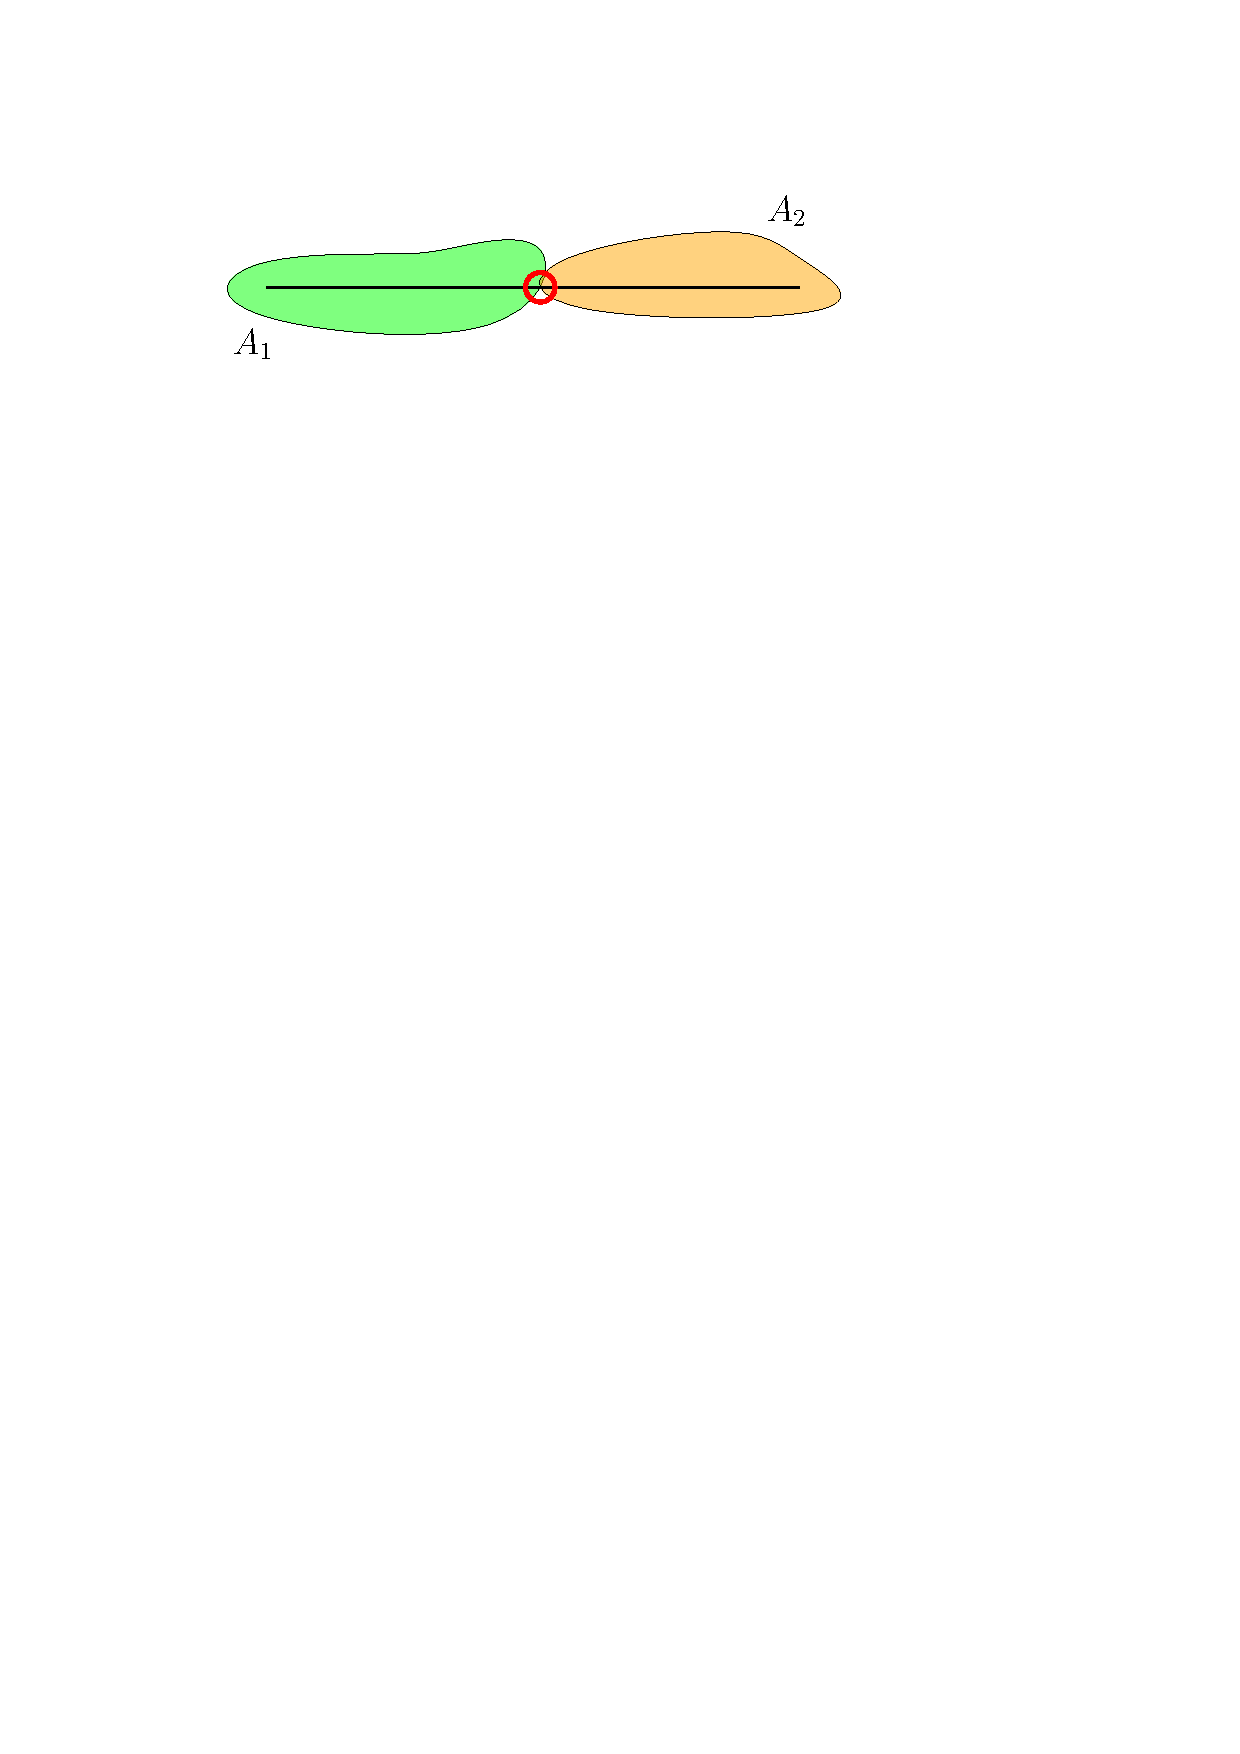
\includegraphics[scale=\normalipe]{ch01-usecka-pokryti-1.pdf}\\\qquad\\
    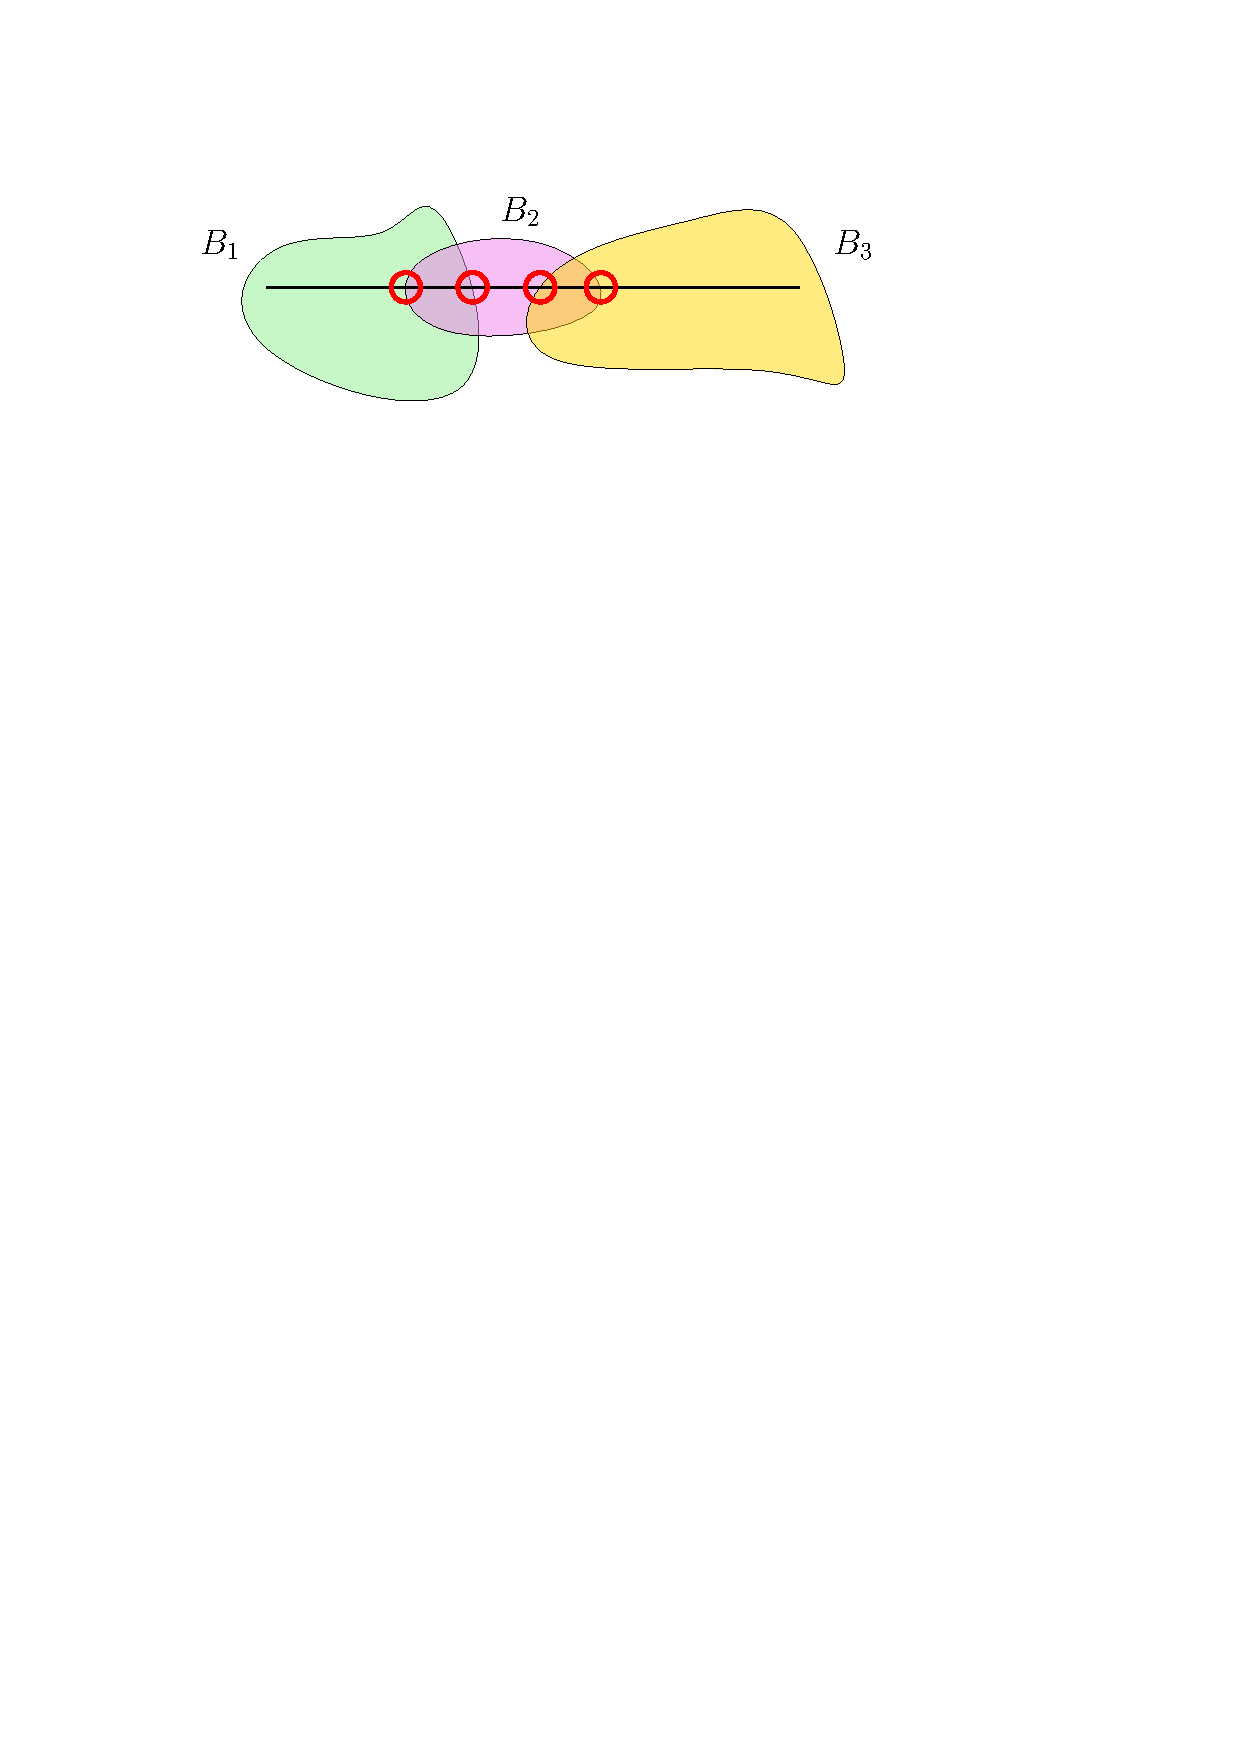
\includegraphics[scale=\normalipe]{ch01-usecka-pokryti-2.pdf}\\\qquad\\
    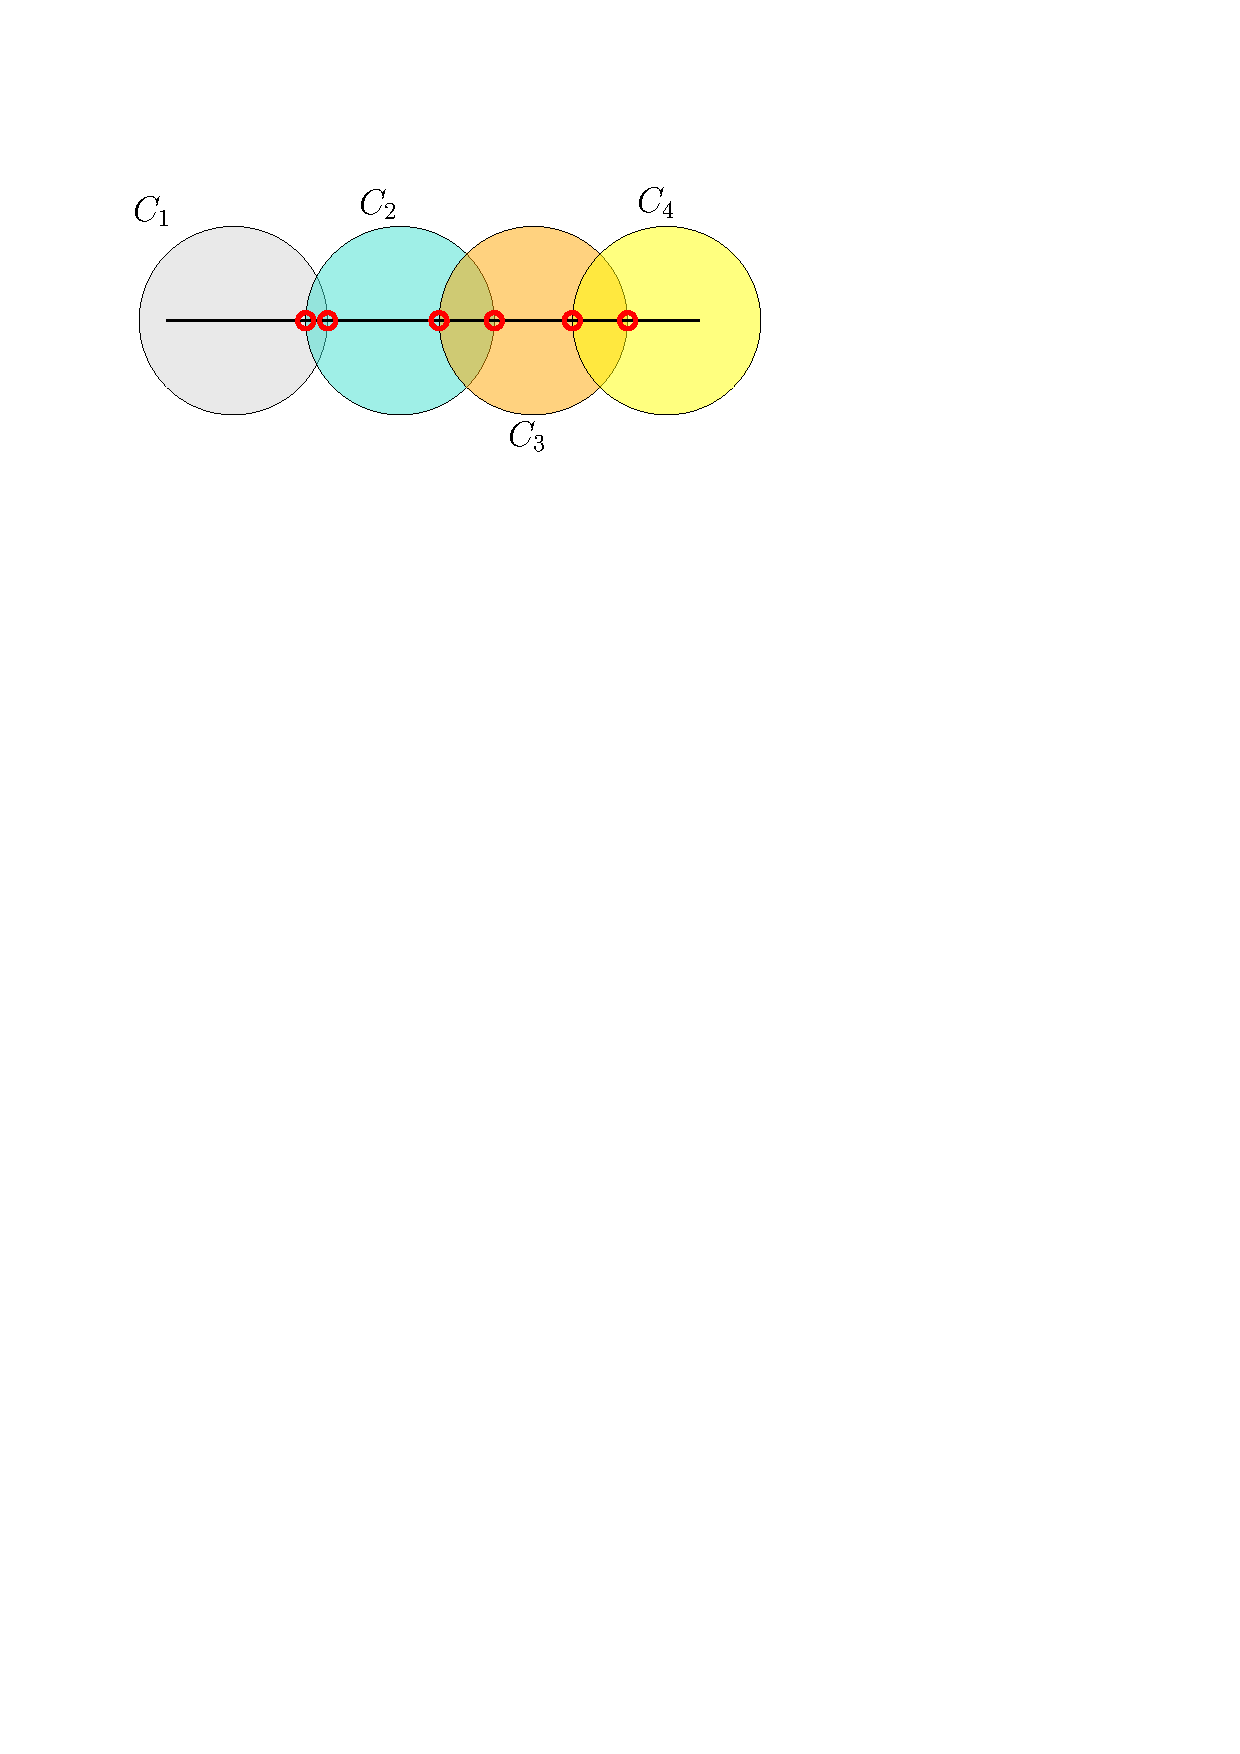
\includegraphics[scale=\normalipe]{ch01-usecka-pokryti-3.pdf}\\\qquad\\
    \caption{Různé možnosti (pod)pokrytí úsečky.}
    \label{fig:usecka-zjemneni}
\end{figure}
Pro libovolné pokrytí lze ukázat,~že každý bod je obsažen maximálně ve \emph{dvou množinách} vhodně zvoleného zjemnění,~tedy topologická dimenze úsečky je $1$. Podobně např. pro čtverec lze dojít k~závěru,~že pro každé pokrytí existuje zjemnění takové,~že každý bod obsažen maximálně ve \emph{třech množinách},~tedy jeho topologická dimenze je 2,~jak bychom očekávali (viz obrázek~\ref{fig:ctverec-zjemneni}).
\begin{figure}[h]
    \centering
    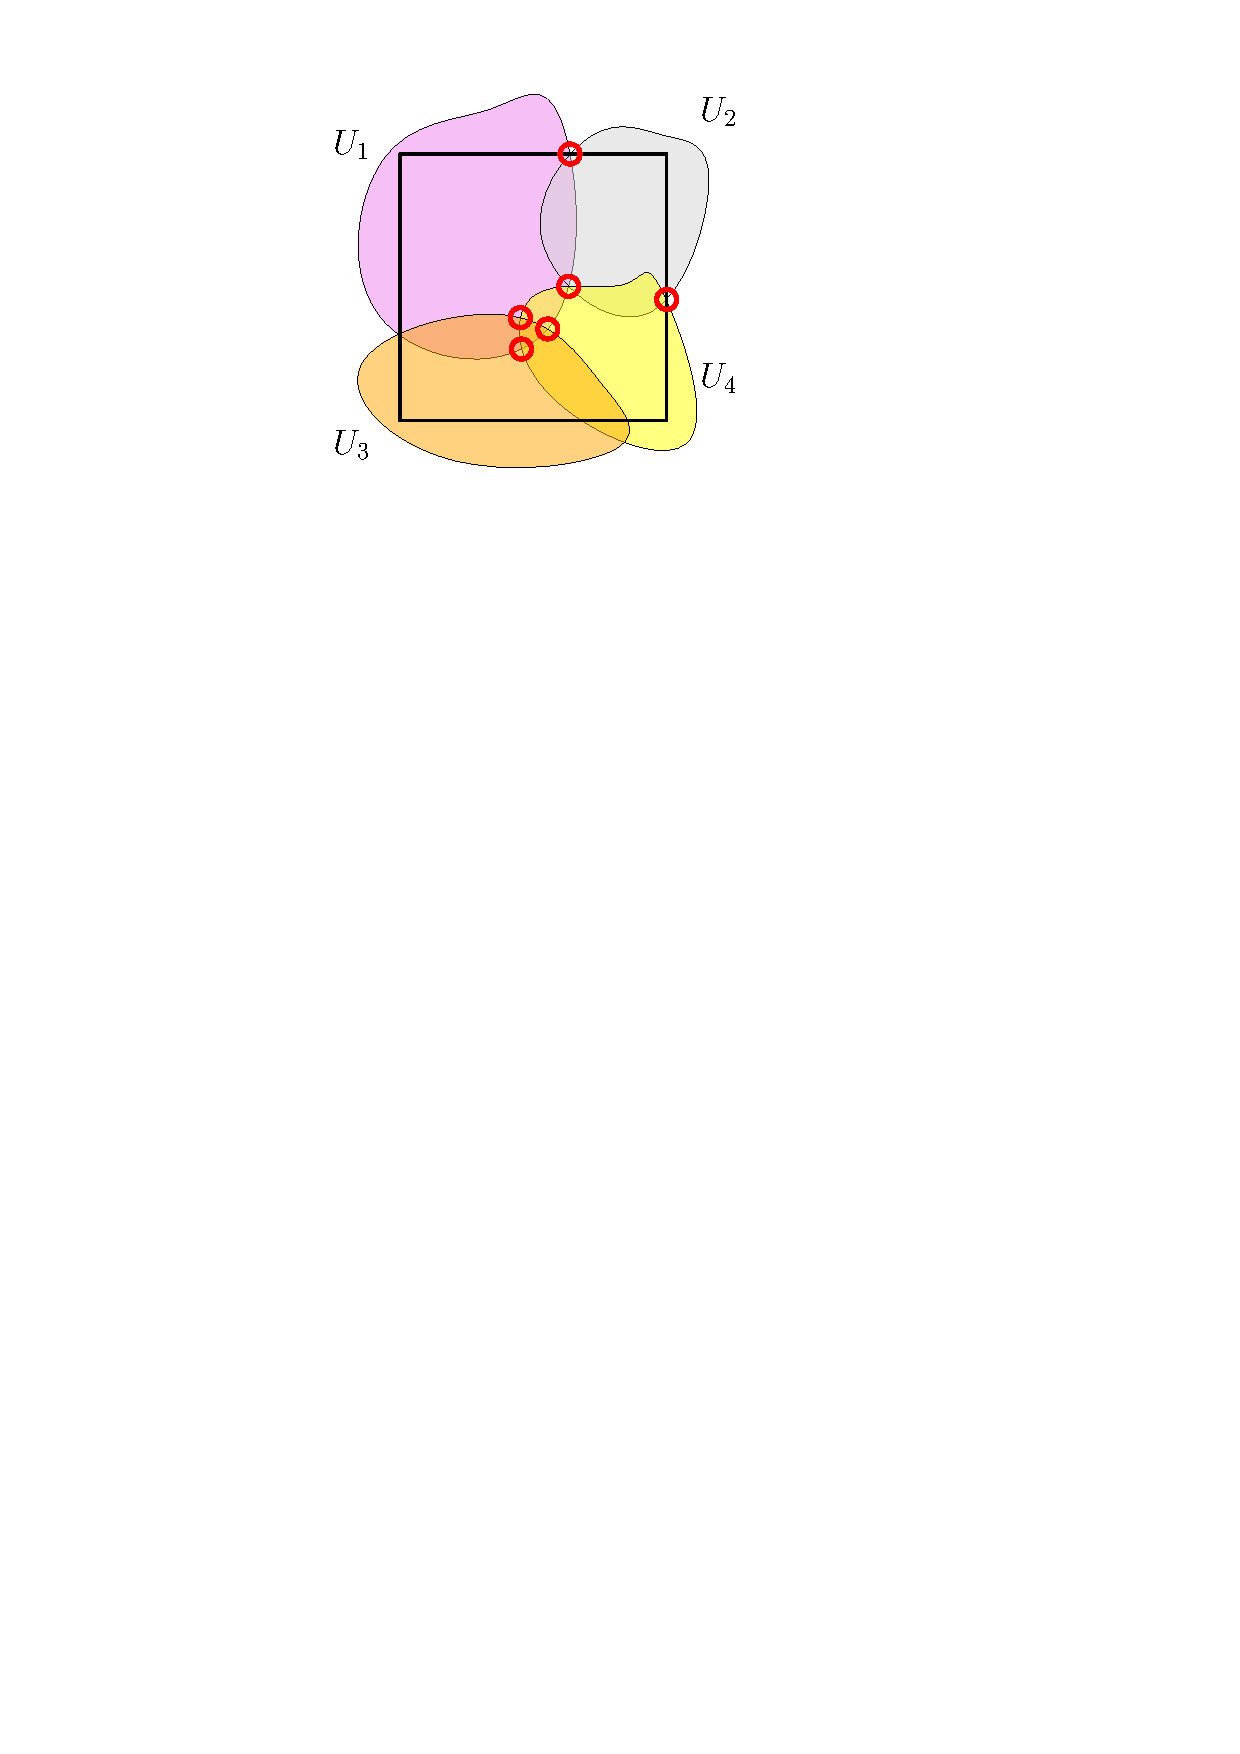
\includegraphics[scale=\normalipe]{ch01-ctverec-pokryti.pdf}
    \caption{Možné (pod)pokrytí čtverce.}
    \label{fig:ctverec-zjemneni}
\end{figure}
Porovnejme nyní topologickou dimenzi vůči dimenzi fraktální. Jak jsme se již přesvědčili v~příkladech~\ref{ex:fraktalni-dimenze-usecka},~\ref{ex:fraktalni-dimenze-ctverec} a~\ref{ex:fraktalni-dimenze-trojuhelnik},~pro "standardní" útvary je fraktální dimenze celočíselná (ač jsou i~další,~které jsme neuvedli),~zatímco v~podsekci~\ref{subsec:dimenze-fraktalu} jsme zjistili,~že u~fraktální dimenze fraktálů tomu tak být nemusí. Přitom však topologická dimenze fraktálních útvarů je (a dokonce musí být) celočíselná (viz tabulka~\ref{table:fraktalni-topologicka-dimenze}).
\begin{table}[h]
    \centering
    \begin{tabular}{r|cc}
    Útvar $F$                & $\dimB{F}$            & $\dimL{F}$ \\\hline
    Úsečka                   & 1                     & 1          \\
    Čtverec                  & 2                     & 2          \\
    Krychle                  & 3                     & 3          \\
    Teserakt                 & 4                     & 4          \\
    $d$-rozměrná krychle     & $d$                   & $d$        \\
    Kochova křivka           & $1{,}2618595\dots$    & 1          \\
    Kochova vločka           & $1{,}2618595\dots$    & 1          \\
    Sierpińského trojúhelník & $1{,}5849625\dots$    & 2          \\
    Cantorovo diskontinuum   & $0{,}6309297\dots$    & 0      
    \end{tabular}
    \caption{Porovnání fraktální a~topologické dimenze útvarů.}
    \label{table:fraktalni-topologicka-dimenze}
\end{table}
Fraktální dimenze tak oproti té topologické daleko lépe zachycuje informaci o~detailní geometrii daných objektů.
\section{Co je to fraktál?}\label{sec:co-je-to-fraktal}
\emph{Tak co je to tedy ten "fraktál"?}\index{fraktál} Odpovědi na tuto otázku jsme se poměrně dlouhou dobu vyhýbali a~onen termín,~popř. jeho přídavnou variantu \emph{"fraktální"},~jsme používali čistě na intuitivní úrovni. Ač jsme se zatím obešli bez jeho formálnějšího upřesnění,~bylo by možná při nejmenším slušné se o~to alespoň pokusit. V~předešlé sekci~\ref{sec:fraktalni_dimenze} jsme pokryli \emph{fraktální} a~\emph{topologickou dimenzi},~které jsme následně použili na příkladech konkrétních útvarů (konkrétně viz tabulky~\ref{table:fraktaly-eukleides-dimenze} a~\ref{table:fraktalni-topologicka-dimenze}).

Již jsme si všimli,~že u~fraktálních útvarů vychází fraktální dimenze $\dimH$ neceločíselně oproti jejich topologické dimenzi $\dimL$,~která je vždy celočíselná. To by se mohlo zdát jako dobrá charakteristika fraktálů. Avšak existují útvary,~jejichž fraktální a~topologická dimenze se shodují,~přestože také mají "fraktální charakter". Pro příklad nemusíme chodit nikterak daleko,~pravděpodobně nejznáměnším útvarem je v~tomto ohledu \emph{Mandelbrotova množina}\index{množina!Mandelbrotova}\index{Mandelbrotova mnozina},~jejiž fraktální i~topologická dimenze je rovna $2$ (blíže se na ni podíváme v~podsekci~\ref{subsec:mandebrotova-mnozina}). Jiná definice zase naopak popisuje fraktál jako útvar,~jehož Hausdorffova dimenze (na tu se blíže podíváme v~sekci~\ref{sec:hausdorffova-mira-dimenze}) je ostře větší než dimenze topologická. Problém (a také důvod,~proč jsme definici toho pojmu vyhývali) je však zkrátka ten,~že dodnes \textbf{není známá} žádná univerzální definice fraktálu. \cite[str. 226]{Voracova2022}

Je to možná lehce zklamávající,~nicméně dobrou zprávou je,~že ani pro další výklad ona absence formální definice fraktálu nebude překážkou. V~dalším textu se zaměříme (mj.) především na jejich klasifikaci (viz kapitola~\ref{chapter:klasifikace-fraktalu}) a~další vlastnosti.
\chapter{Teorie míry a dimenze}\label{chapter:teorie-miry-a-dimenze}

V této kapitole se budeme nyní věnovat fraktálům a jim příbuzným záležitostem trochu formálněji. Do této chvíle jsme si již stihli představit některé základní fraktály,~jako je např. \emph{Sierpińského trojúhelník},~\emph{Kochova vločka} nebo \emph{Cantorovo diskontinuum},~na nichž jsme si ilustrovali především myšlenku soběpodobnosti a na to navazující pojetí dimenze (viz kapitola \ref{chapter:uvod_do_fraktalu},~sekce \ref{sec:sobepodobnost} a \ref{sec:fraktalni_dimenze}).

Ačkoliv leckterý čtenář by se s~poskytnutým vysvětlením jistě spokojil,~jiný by mohl namítat,~že jsme řadu věcí vynechali. A měl by jistě pravdu. Proto se v~této kapitole budeme věnovat některým záležitostem z tzv. \emph{teorie míry}\index{teorie míry},~která je v~tomto ohledu klíčová a poskytne nám nástroje pro měření fraktálních útvarů,~jejichž geometrie často přesahuje možnosti klasické "eukleidovské analýzy". \emph{Míra} pro nás představuje zobecnění pojmů jako je \emph{délka,~obsah} a \emph{objem},~které známe ze školní geometrie. Na jejím základě pak budeme schopni detailněji prozkoumat fraktální dimenzi,~kterou jsme již v~základu pokryli v~předešlé kapitole. Jmenovitě se budeme zabývat
\begin{itemize}
    \item \emph{měřitelnými prostory} a \emph{prostory s mírou} obecně,
    \item \emph{box-counting dimenzí}\footnote{Též ji lze nalézt pod~názvem \emph{Minkowského dimenze} nebo \emph{Minkowského-Bouligandova dimenze}. Je pojmenována po polském matematikovi \name{Hermannovi Minkowském} (1864--1909) a francouzském matematikovi \name{Georgesovi Bouligandovi} (1889--1979).}
    \item \emph{Hausdorffovou mírou} a z ní vycházející \emph{Hausdorffovou dimenzí}.
\end{itemize}

Ačkoliv je toto téma jinak velice obsáhlé jsou mu věnované samostatné texty i~knihy,~spokojíme se pouze s~naprostým základem. Pro další znalosti si dovolím čtenáře odkázat na knihy \cite{Falconer2014},~\cite{Lukes2013} a \cite{Netuka2016}.

\section{Základní pojmy a značení}\label{sec:zakladni-pojmy-a-znaceni}

V tomto oddílu se v~krátkosti zaměříme na připomenutí některých pojmů a značení,~které budeme dále využívat. Související teorii týkající se mnoha záležitostí v~tomto případě vynecháme s~předpokladem,~že ji čtenář již zná. Pokud tomu však v~některých případech takto nebude,~lze tuto část textu považovat za výčet konceptů,~které pro zvládnutí nadcházející teorie budeme potřebovat.

\todo{Doplnit pojmy a značení podle dalšího textu
    \begin{itemize}
        \item Limita funkce
        \item Limes superior/inferior
        \item Metrický prostor, úplný MP
        \item Cauchyovská posloupnost
        \item vzdálenost bodu od množiny
        \item Otevřená/uzavřená koule
        \item Otevřená/uzavřená množina
        \item Kompaktní množina, věta o kompaktnosti v $\R^n$, věta o uzavřenosti kompaktní množiny.
        \item Kvádr a objem kvádru
        \item Průměr množiny
        \item $\delta$-okolí množiny
        \item Pokrytí, zjemnění
        \item $\delta$-pokrytí
        \item $\delta$-mříž
        \item Vnitřek, hranice množiny
        \item (bi-)lipschitzovské zobrazení
    \end{itemize}
}
\section{Prostory s~mírou}\label{sec:prostory-s-mirou}

Jak již bylo zmíněno v~úvodu,~klíčovým pojmem v~této kapitole (a pro studium fraktálů obecně) je takzvaná \emph{míra}. Ta pro nás představuje obecný způsob,~jak můžeme množinám přiřadit v~jistém smyslu "velikost". Konkrétněji,~byť vágně,~lze říci,~že sestává-li množina z~konečného nebo spočetného množství "rozumných" částí,~pak součet velikostí všech těchto dílčích množin je roven velikosti celé množiny,~kterou nazveme její \emph{mírou}. Pro začátek celkem jednoduchá myšlenka.

Pro formální zavedení tohoto pojmu však budeme muset nejprve zavést ještě jiný pojem,~a to tzv. \emph{$\sigma$-algebru}.

\subsection{Měřitelné prostory}\label{subsec:meritelne-prostory}

\begin{definition}[$\sigma$-algebra]\label{def:sigma-algebra}
    Nechť je dána libovolná množina $X$ a systém podmnožin $\mathcal{A}\subseteq\powset{X}$. Pak $\mathcal{A}$ je \emph{$\sigma$-algebra}\index{$\sigma$-algebra} na množině $X$,~pokud:
    \begin{enumerate}[label=(\alph*)]
        \item\label{def:sigma-algebra-podm1} $X\in\mathcal{A}$.
        \item\label{def:sigma-algebra-podm2} Pro každou množinu $A\in\mathcal{A}$ platí $X\setminus A\in\mathcal{A}$.
        \item\label{def:sigma-algebra-podm3} Pro libovolné množiny $A_1,A_2,\ldots\in\mathcal{A}$ platí $\bigcup_{i=1}^\infty A_i\in\mathcal{A}$.
    \end{enumerate}
    Dvojice $(X,\mathcal{A})$ se nazývá měřitelný prostor\index{prostor!měřitelný}.
\end{definition}

\begin{example}
    Jednoduché příklady $\sigma$-algeber:
    \begin{itemize}
        \item Triviálními příklady $\sigma$-algeber jsou množiny $\emptyset$,~$\powset{X}$ a~$\set{\emptyset,X}$ pro libovolnou množinu $X$.
        \item Pro konečnou množinu $X=\set{a,b,c,d}$ je jednou možnou $\sigma$-algebrou systém množin
        \[\Sigma=\set{\emptyset,\set{a,b},\set{c,d},\set{a,b,c,d}}.\]
    \end{itemize}
    Sami se zkuste přesvědčit,~že všechny zmíněné příklady vyhovují definici \ref{def:sigma-algebra}.
\end{example}

Než vyslovíme něco dalšího o~$\sigma$-algebrách a jejich významu,~podíváme se na seznam některých vesměs jednoduchých pozorováních zformulovaných níže v~tvrzení \ref{thm:sigma-algebra-vlastnosti}.
\begin{theorem}[Vlastnosti $\sigma$-algebry]\label{thm:sigma-algebra-vlastnosti}
    Nechť $(X,\mathcal{A})$ je meřitelný prostor. Pak platí:
    \begin{enumerate}[label=(\roman*)]
        \item $\emptyset\in\mathcal{A}$.
        \item Pro libovolné množiny $A_1,A_2,\ldots\in\mathcal{A}$ platí $\bigcap_{i=1}^\infty A_i\in\mathcal{A}$.
        \item Pro všechny množiny $A_1,A_2,\ldots,A_n\in\mathcal{A}$ platí
        \[\bigcup_{i=1}^n A_i\in\mathcal{A}\land\bigcap_{i=1}^n A_i\in\mathcal{A}.\]
        \item Jsou-li $A,B\in\mathcal{A}$ pak $A\setminus B\in\mathcal{A}$.
    \end{enumerate}
\end{theorem}

Z tohoto tvrzení je již lépe vidět,~proč jsou pro nás $\sigma$-algebry tak příjemným objektem. Jsou totiž \emph{uzavřené} na všechny základní množinové operace. To se nám bude později hodit při zavedení míry,~ke které směřujeme. Důkaz těchto dílčích tvrzení přitom není nikterak složitý.
\begin{proof}
    Mějme $\sigma$-algebru $\mathcal{A}$ na množině $X$.
    \begin{enumerate}[label=\textit{(\roman*)}]
        \item Z~podmínky \ref{def:sigma-algebra-podm1} definice \ref{def:sigma-algebra} víme,~že $X\in\mathcal{A}$ a z~podmínky \ref{def:sigma-algebra-podm2} tedy plyne $X\setminus X=\emptyset\in\mathcal{A}$.
        \item Mějme množiny $A_1,A_2,\ldots\in\mathcal{A}$. Společně s~využitím De Morganových zákonů plyne následující:
        \[\bigcap\limits_{i=1}^\infty A_i=\overbrace{X\setminus\underbrace{\bigcup\limits_{i=1}^\infty \overbrace{(X\setminus A_i)}^{\text{$\in\mathcal{A}$ podle \ref{def:sigma-algebra-podm2}}}}_{\text{$\in\mathcal{A}$ podle \ref{def:sigma-algebra-podm3}}}}^\text{$\in\mathcal{A}$ podle \ref{def:sigma-algebra-podm2}}\in\mathcal{A}.\]
        \item Nechť jsou dány množiny $A_1,A_2,\ldots,A_n\in\mathcal{A}$. Když pro každé $j>n$ položíme $A_j=\emptyset$,~pak platí
        \[\bigcup\limits_{i=1}^n A_i=\bigcup\limits_{i=1}^\infty A_i\in\mathcal{A}\]
        a podobně pro $\bigcap_{i=1}^n A_i\in\mathcal{A}$ podle předešlého bodu.
        \item Pro libovolné množiny $A,B\in\mathcal{A}$ platí
        \[A\setminus B=\overbrace{A\cup\underbrace{(X\setminus B)}_{\text{$\in\mathcal{A}$ podle \ref{def:sigma-algebra-podm2}}}}^{\text{$\in\mathcal{A}$ podle \ref{def:sigma-algebra-podm3}}}\in\mathcal{A}.\]
    \end{enumerate}
\end{proof}

\subsection{Míra}\label{subsec:mira}

V tuto chvíli máme již vše potřebné k~zavedení pojmu míra,~resp. prostor s~mírou.
\begin{definition}[Prostor s~mírou]\label{def:prostor-s-mirou}
    Nechť $(X,\mathcal{A})$ je měřitelný prostor. Zobrazení $\mapping{\mu}{\mathcal{A}}{\langle0,\infty\rangle}$ se nazývá \emph{míra}\index{míra} na $\mathcal{A}$,~pokud platí:
    \begin{enumerate}[label=(\alph*)]
        \item\label{def:mira-podm1} $\mu(\emptyset)=0$,
        \item\label{def:mira-podm2} pro množiny $A_1,A_2,\ldots$, kde $A_i\in\mathcal{A}$ pro každé $i\in\N$, po dvou disjunktní je
        \[\mu\left(\bigcup\limits_{i=1}^\infty A_i\right)=\sum_{i=1}^\infty\mu(A_i).\mathrightnote{$\sigma$-aditivita}\]
    \end{enumerate}
    Uspořádanou trojici $(X,\mathcal{A},\mu)$ nazýváme \emph{prostor s~mírou}\index{prostor!s mírou}\index{prostor s~mírou}.
\end{definition}

Vzhledem k~tomu,~co míra reprezentuje (tj. zobecnění délky,~obsahu,~objemu),~jsou tyto požadavky intuitivně dosti smysluplné.

\begin{example}\label{ex:mira}
    Příklady prostorů s~mírou:
    \begin{itemize}
        \item Asi pro nás nejtypičtější způsob,~jak měřit "velikost" množiny,~je podle \emph{počtu prvků}. Pro libovolnou množinu $X$ a potenční množinu $\powset{X}$ lze definovat prostor s~mírou $(X,\powset{X},\mu)$,~kde pro libovolnou množinu $A\in\powset{X}$ položíme $\mu(A)=|A|$. Takto definované míře $\mu$ říkáme \emph{aritmetická míra}\index{míra!aritmetická}.
        \item Máme libovolnou množinu $X$ a $\sigma$-algebru $\mathcal{A}$. Zvolme si pevně $x\in X$. Míru libovolné množiny $A\in\mathcal{A}$ lze definovat jako $\delta_x(A)=\chi_A(x)$,~kde $\chi_A$ je charakteristická funkce množiny $A$. Zobrazení $\delta_x$ je tzv. \emph{Diracova míra}\index{míra!Diracova}.
        \item Zobrazení přiřazující náhodnému jevu pravděpodobnost je též případem míry. Označíme-li si $\Omega=\set{\omega_1,\omega_2,\ldots,\omega_n}$ množinu všech elementárních jevů a $\mathcal{F}\subseteq\powset{\Omega}$,~pak $\mapping{\mathsf{P}}{\mathcal{F}}{\langle0,1\rangle}$ definovaná pro $A\in\mathcal{F}$ jako
        \[\mathsf{P}(A)=\dfrac{|A|}{|\Omega|}\]
        je mírou na $\mathcal{F}$. Speciálně $\mathsf{P}(\Omega)=1$.
    \end{itemize}
\end{example}

Ve všech případech zobrazení $\mu$ v~příkladu \ref{ex:mira} se lze snadno přesvědčit,~že se jedná o~míru,~tedy že splňuje podmínky \ref{def:mira-podm1} a \ref{def:mira-podm2} uvedené v~definici \ref{def:prostor-s-mirou} výše.

Pojďme nyní prozkoumat vlastnosti míry trochu hlouběji.
\begin{theorem}[Vlastnosti míry]\label{thm:mira-vlastnosti}
    Nechť $\mu$ je míra na $\sigma$-algebře $\mathcal{A}$. Pak platí následující:
    \begin{enumerate}[label=(\roman*)]
        \item\label{thm:mira-aditivita} Jsou-li množiny $A_1,A_2,\ldots,A_n\in\mathcal{A}$ po dvou disjunktní,~pak
        \[\mu\left(\bigcup_{i=1}^n A_i\right)=\sum_{i=1}^{n}\mu(A_i).\mathrightnote{aditivita\index{aditivita}}\]
        \item\label{thm:mira-monotonie} Pokud $A,B\in\mathcal{A}$ a $A\subseteq B$,~pak
        \[\mu(A)\leqslant\mu(B).\mathrightnote{monotonie míry\index{monotonie míry}}\]
        Navíc pokud $\mu(A)<\infty$,~pak $\mu(B\setminus A)=\mu(B)-\mu(A)$.
        \item\label{thm:mira-nekl-posl} Pokud $A_1,A_2,\ldots$,~kde $A_i\in\mathcal{A}$ pro každé $i\in\N$,~je neklesající posloupnost množin\footnote{Posloupnost množin,~kde $A_i\subseteq A_{i+1}$ pro každé $i\in\N$.},~pak
        \[\lim_{j\to\infty}\mu(A_j)=\mu\left(\bigcup_{j=1}^\infty A_j\right).\]
        \item\label{thm:mira-nerost-posl} Pokud $A_1,A_2,\ldots$, kde $A_i\in\mathcal{A}$ pro každé $i\in\N$, je nerostoucí posloupnost množin\footnote{$A_i\supseteq  A_{i+1}$ pro každé $i\in\N$.} a~navíc $\mu(A_1)<\infty$,~pak
        \[\lim_{j\to\infty}\mu(A_j)=\mu\left(\bigcap_{j=1}^\infty A_j\right).\]
        \item\label{thm:mira-sigma-subaditivita} Pokud $A_1,A_2,\ldots$,~kde $A_i\in\mathcal{A}$ pro každé $i\in\N$,~pak
        \[\mu\left(\bigcup_{i=1}^\infty A_i\right)\leqslant\sum_{i=1}^{\infty}\mu(A_i).\mathrightnote{$\sigma$-subaditivita}\]
    \end{enumerate}
\end{theorem}

Poslední vlastnost \ref{thm:mira-sigma-subaditivita} je tzv. \emph{$\sigma$-subaditivita}\index{$\sigma$-subaditivita}\footnote{V matematické terminologii se předpona $\sigma$ běžně týká spočetných sjednocení. \citep[str. 2]{Lukes2013}}. Oproti $\sigma$-aditivitě\index{$\sigma$-aditivita} se liší tím,~že u~množin $A_1,A_2,\dots$ se nepožaduje,~aby byly po dvou disjunktní,~tzn. mohou se "překrývat". Je však intuitivně nejspíše jasné,~že součtem měr všech těchto množin určitě nemůžeme získat míru nižší než je míra jejich sjednocení (dané "překryvy" započítáváme v~sumě vícekrát). Podobně i~monotonie dává intuitivně smysl,~neboť část větší množiny jistě nemůže mít větší míru než celek. Na formální stránku věci se podíváme nyní.
\begin{proof}
    V~důkazu využijeme některé vlastnosti $\sigma$-algebry z~věty \ref{thm:sigma-algebra-vlastnosti},~zejména,~že všechny množiny níže jsou opět prvky $\sigma$-algebry~$\mathcal{A}$.
    \begin{enumerate}[label=\textit{(\roman*)}]
        \item Pokud pro každé $j>n$ položíme $A_j=\emptyset$,~pak z~definice míry plyne
        \[\mu\left(\bigcup_{i=1}^n A_i\right)=\mu\left(\bigcup_{i=1}^\infty A_i\right)=\sum_{i=1}^{\infty}\mu(A_i)=\sum_{i=1}^{n}\mu(A_i).\]
        \item Nechť jsou dány $A,B\in\mathcal{A}$,~takové,~že $A\subseteq B$. Pak $B=A\cup(B\setminus A)$,~přičemž $A$ a $B\setminus A$ jsou disjunktní. Tedy podle bodu \ref{def:mira-podm2} lze psát $\mu(B)=\mu(A)+\mu(B\setminus A)\geqslant\mu(A)$,~protože $\mu(B\setminus A)\geqslant 0$.
        \item Mějme neklesající posloupnost množin $A_1,A_2,\ldots$,~kde $A_i\in\mathcal{A}$ pro každé $i\in\N$ (viz obrázek \ref{fig:nekl-posl-mnozin}).
        Definujeme posloupnost\footnote{V podstatě konstruujeme množiny $A_1,A_2,\ldots$ tak,~aby v~následující množině $A_i$ nebyl obsažen prvek,~který se nachází již v~některé z~množin $A_1,A_2,\ldots,A_{i-1}$. Podobná myšlenka je využita i~při důkazu budů \ref{thm:mira-nerost-posl} a \ref{thm:mira-sigma-subaditivita}.} množin $B_1,B_2,\ldots$ následovně:
        \[B_1=A_1,\;B_2=A_2\setminus A_1,\;B_i=A_i\setminus A_{i-1},\;i\geqslant 2.\]
        Množiny $B_1,B_2,\dots$ jsou po dvou disjunktní a zároveň\\$\bigcup_{i=1}^\infty B_i=\bigcup_{i=1}^\infty A_i$. Libovolnou množinu $A_n$ lze totiž zapsat jako
        \[A_n=\bigcup_{i=1}^n (A_i\setminus A_{i-1})=\bigcup_{i=1}^n B_i.\] 
        Podle již dokázaného bodu \ref{thm:mira-aditivita} (aditivita míry) tedy pro každé $n$ platí $\mu(A_n)=\sum_{i=1}^{n}\mu(B_i)$.
        Celkově
        \[\mu\left(\bigcup_{i=1}^\infty A_i\right)=\mu\left(\bigcup_{i=1}^\infty B_i\right)=\sum_{i=1}^{\infty}\mu(B_i)=\lim_{n\to\infty}\sum_{i=1}^{n}\mu(B_i)=\lim_{n\to\infty}\mu(A_n).\]
        \item Nechť je dána nerostoucí posloupnost množin $A_1,A_2,\ldots$,~kde $A_i\in\mathcal{A}$ pro každé $i\in\N$ (viz obrázek \ref{fig:nerost-posl-mnozin}). Podobně jako v~předešlém bodě,~i~zde definujeme novou posloupnost množin $B_1,B_2,\ldots$ takto:
        \[B_i=A_1\setminus A_i,\;i\in\N.\]
        Zde si můžeme všimnout,~že pro každé $i$ platí $B_i\subseteq B_{i+1}$ a splňuje tak předpoklad předešlého bodu \ref{thm:mira-nekl-posl}. Dle De Morganových zákonů můžeme psát
        \[\bigcup_{i=1}^\infty B_i=\bigcup_{i=1}^\infty(A_1\setminus A_i)=A_1\setminus\bigcap_{i=1}^\infty A_i.\]
        Výraz $\lim_{j\to\infty}B_j$ lze rozepsat dvěma způsoby:
        \begin{align*}
            \lim\limits_{j\to\infty}\mu(B_j)&\stackrel{\ref{thm:mira-nekl-posl}}{=}\mu\left(\bigcup\limits_{i=1}^\infty B_i\right)=\mu\left(A_1\setminus\bigcap\limits_{i=1}^\infty A_i\right)\stackrel{\ref{thm:mira-monotonie}}{=}\mu(A_1)-\mu\left(\bigcap\limits_{i=1}^\infty A_i\right),\\
            \lim\limits_{j\to\infty}\mu(B_j)&=\lim_{j\to\infty}(A_1\setminus A_j)\stackrel{\ref{thm:mira-monotonie}}{=}\lim_{j\to\infty}(\mu(A_1)-\mu(A_j))=\mu(A_1)-\lim_{j\to\infty}\mu(A_j).
        \end{align*}
        Porovnáním obou rovností lze vidět,~že
        \[\lim_{j\to\infty}\mu(A_j)=\mu\left(\bigcap\limits_{i=1}^\infty A_i\right).\]
        \item Nechť jsou dány množiny $A_1,A_2,\ldots$,~kde $A_i\in\mathcal{A}$ pro každé $i\in\N$. Definujeme posloupnost množin $B_1,B_2,\ldots$ takto:
        \[B_1=A_1,\;B_k=A_k\setminus\bigcup_{i=1}^{k-1} A_i,\;k\leqslant 2.\]
        (Viz obrázek \ref{fig:vlastnosti-miry-bod-v}.) Není složité si rozmyslet,~že množiny $B_1,B_2,\ldots$ jsou po dvou disjunktní. Zároveň platí $\bigcup_{i=1}^\infty B_i=\bigcup_{i=1}^\infty A_i$ a $B_j\subseteq A_j$ pro každé $j\in\N$. Tím je dokázáno,~že
        \[\mu\left(\bigcup_{i=1}^\infty A_i\right)=\mu\left(\bigcup_{i=1}^\infty B_i\right)=\sum_{i=1}^{\infty}\mu(B_i)\stackrel{\ref{thm:mira-monotonie}}{\leqslant}\sum_{i=1}^{\infty}\mu(A_i).\]
    \end{enumerate}
    \begin{figure}[h]
        \centering
        \begin{subfigure}{0.45\textwidth}
            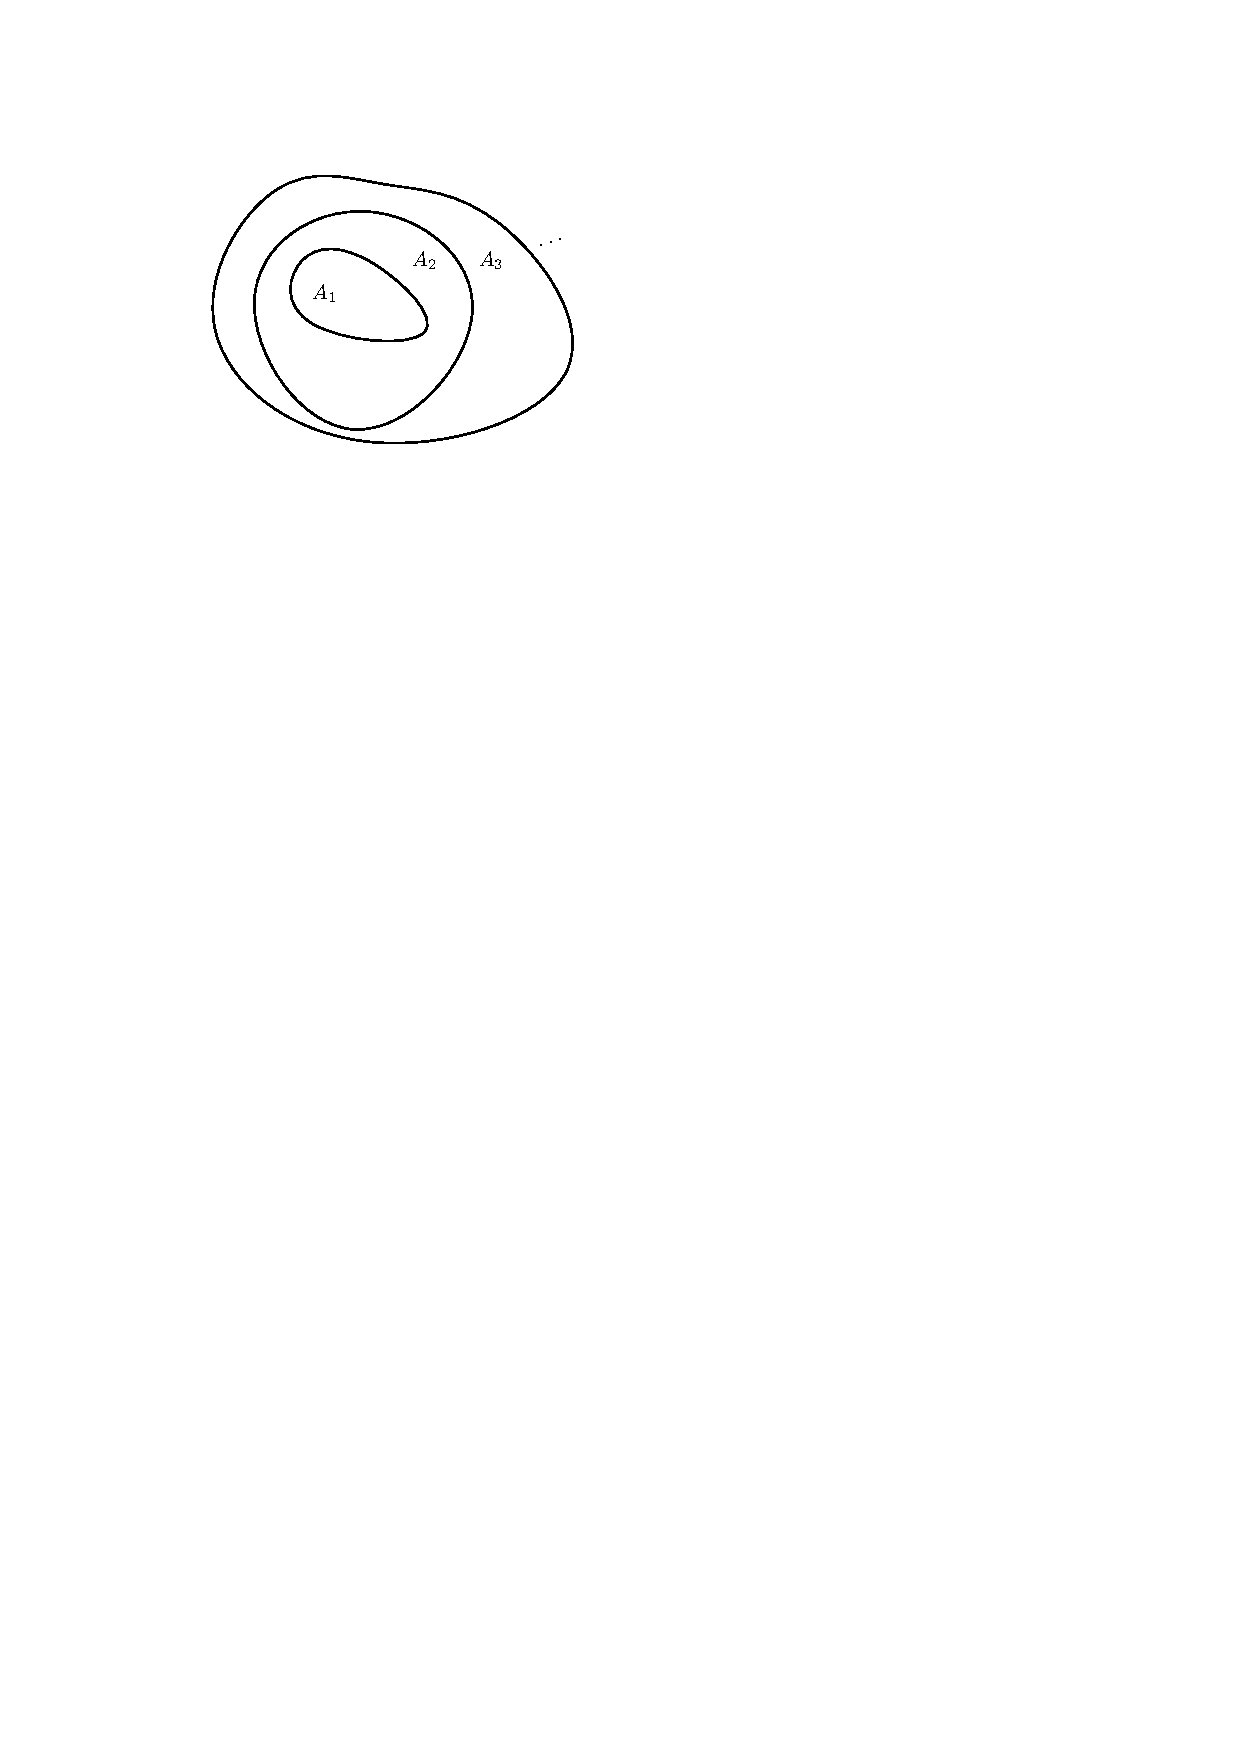
\includegraphics{ch02-neklesajici-posl-mnozin.pdf}
            \caption{Neklesající posloupnost množin}
            \label{fig:nekl-posl-mnozin}
        \end{subfigure}
        \qquad
        \begin{subfigure}{0.45\textwidth}
            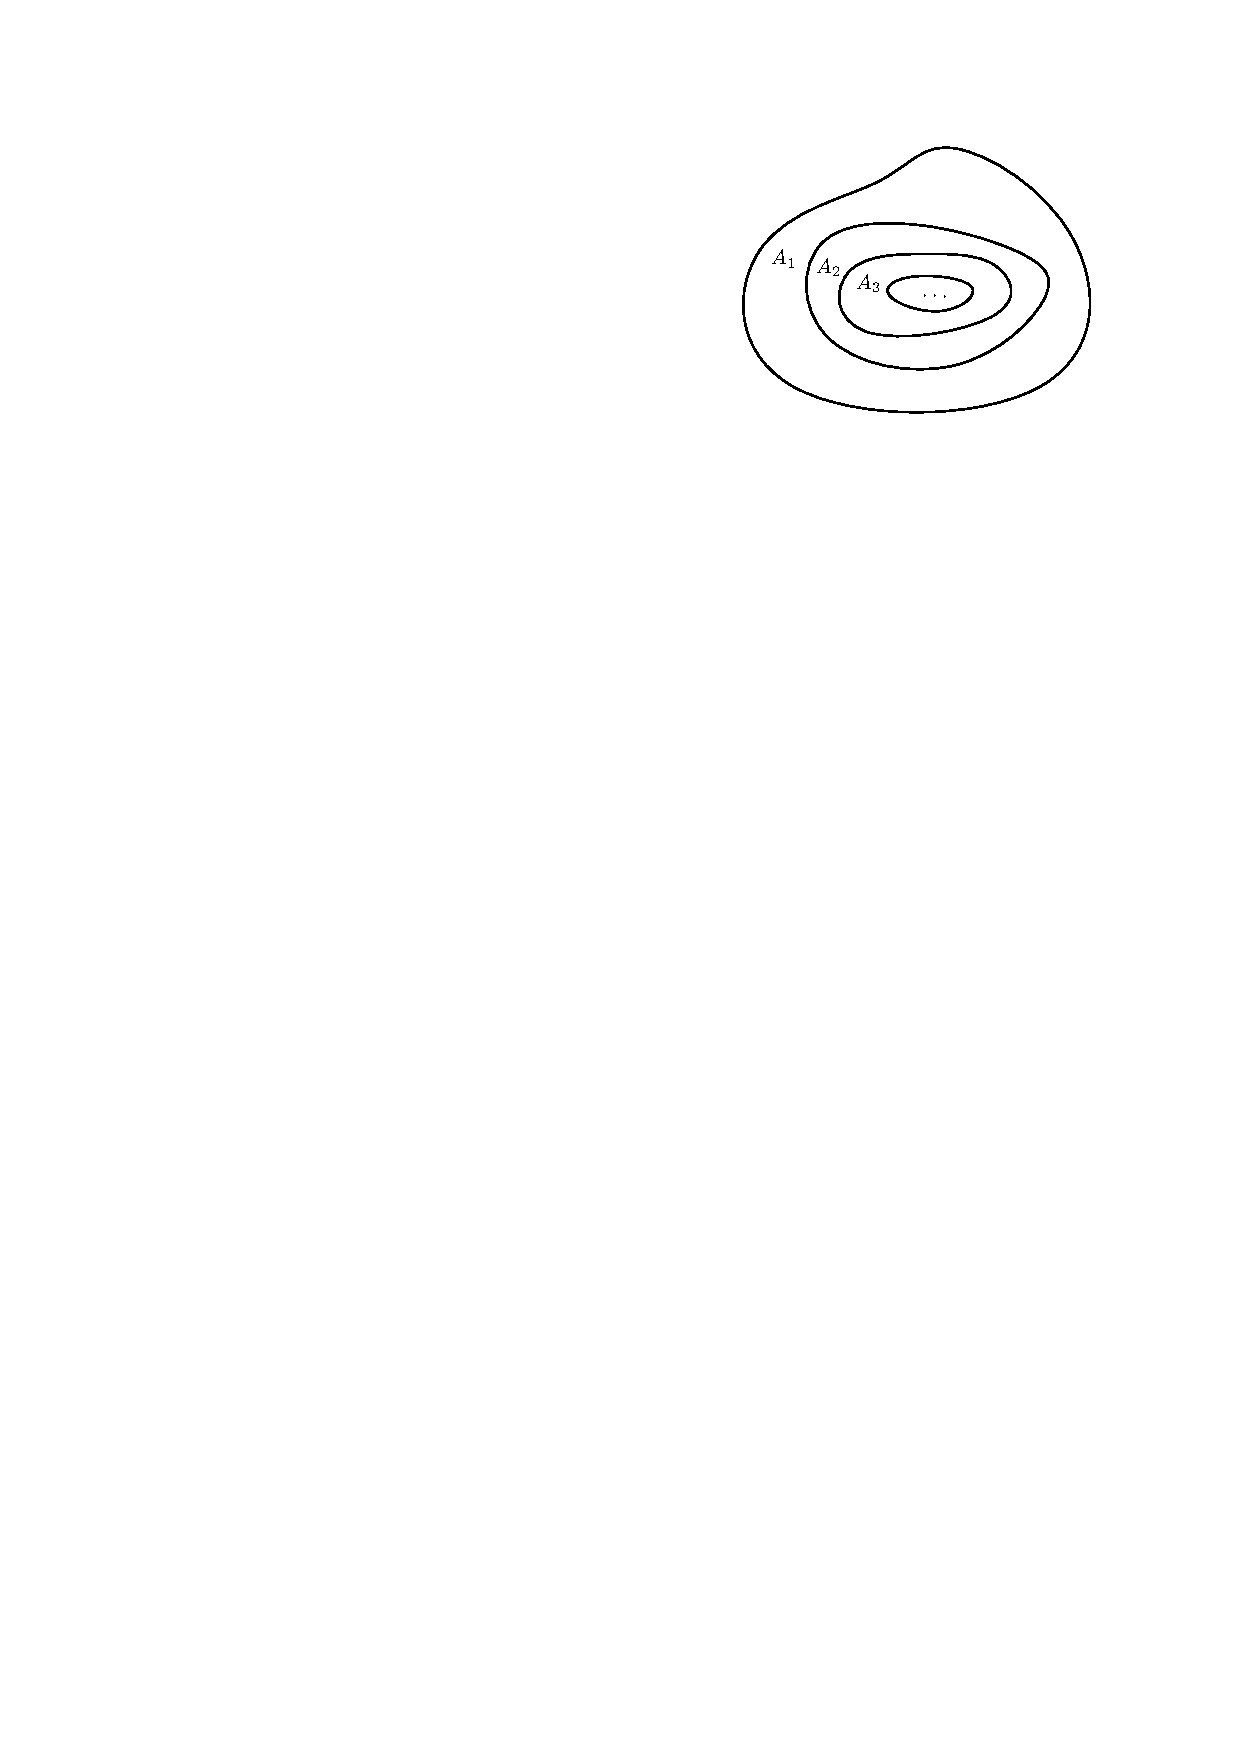
\includegraphics{ch02-nerostouci-posl-mnozin.pdf}
            \caption{Nerostoucí posloupnost množin}
            \label{fig:nerost-posl-mnozin}
        \end{subfigure}
        %% Problém s~PDF/A
        \begin{subfigure}{0.45\textwidth}
            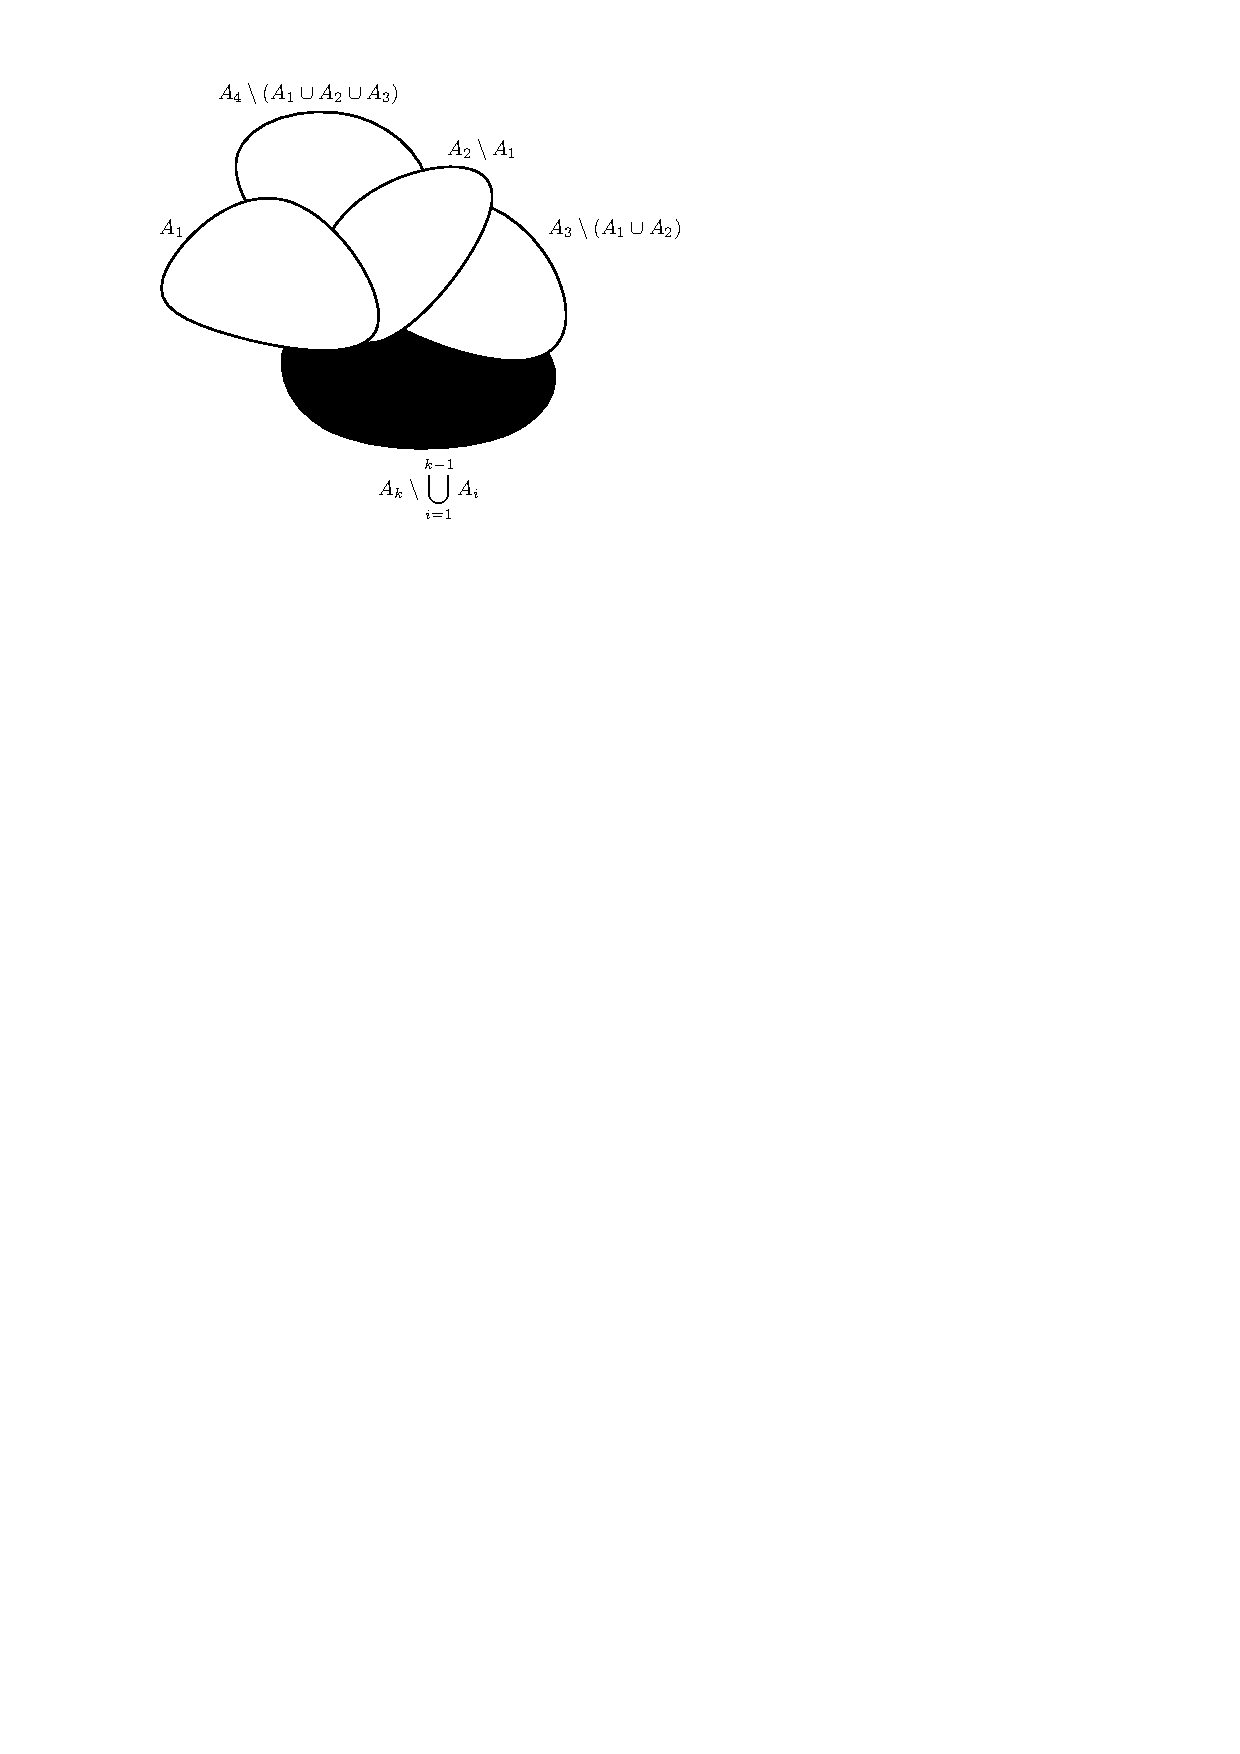
\includegraphics{ch02-vlastnosti-miry-bod-v.pdf}
            \caption{Konstrukce množin $B_k$}
            \label{fig:vlastnosti-miry-bod-v}
        \end{subfigure}
        \caption{Ilustrace k~důkazu věty \ref{thm:mira-vlastnosti}}
    \end{figure}
    (Převzato z~\citep[str. 19]{NetukaIntegral2016})
\end{proof}
\begin{remark}
    Předpoklad $\mu(A_1)<\infty$ ve větě \ref{thm:mira-vlastnosti} v~bodě \ref{thm:mira-nerost-posl} nelze vynechat. Jednoduchý protipříklad si uvedeme v~sekci \ref{sec:lebesgueova-mira}.
\end{remark}
\section{Lebesgueova míra}\label{sec:lebesgueova-mira}

\todo{Doplnit zmínku o Jordanově-Peanově obsahu}

V předešlé sekci \ref{sec:prostory-s-mirou} jsme se povídali o pojmu \emph{míra} obecně a podívali jsme se na několik příkladů. Obecnou ideu měření "velikosti" lze založit např. na aproximaci obecné množiny pomocí \emph{spočetných sjednocení útvarů}, jejichž "velikost" umíme jednoduše určit. V dalším textu se omezíme pouze na množinu $\R^n$.

Na zmíněné myšlence je postavena definice tzv. \emph{$n$-rozměrné Lebesgueovy míry}, kdy obecnou množinu budeme pokrývat pomocí \emph{kvádrů}. Připomeňme, že obecně \mbox{$n$-rozměrným} kvádrem\index{$n$-rozměrný kvádr} $I$ rozumíme kartézský součin \emph{intervalů}
\[\langle a_1,b_1\rangle,\ldots,\langle a_n,b_n\rangle\subseteq\R,\]
tj.
\[I=\prod_{i=1}^{n}\langle a_i,b_i\rangle=\langle a_1,b_1\rangle\times\langle a_2,b_2\rangle\times\dots\times\langle a_n,b_n\rangle\]
a jeho objem\index{kvádr!objem kvádru} definujeme jako
\[\vol^n(I)=\prod_{i=1}^{n}(b_i-a_i).\]
Nyní si definujeme tzv. \emph{vnější Lebesgueovu míru}.
\begin{definition}[Vnější Lebesgueova míra]\label{def:vnejsi-lebegueova-mira}
    Nechť $A\subseteq\R^n$. Pak vnější $n$-rozměr\-nou Lebesgueovou mírou\index{vnější $n$-rozměrná Lebesgueova míra} $A$ je
    \[\lambda_n^*(A)=\inf\set{\sum_{j=1}^{\infty}\vol^n(I_j)\;\middle|\;\text{$I_j$ je kvádr}\land A\subseteq\bigcup_{i=1}^\infty I_j}.\]
\end{definition}
Vnější Lebesgueova míra množiny intuitivně zachycuje informaci o "velikosti" dané množiny.  Lze ihned vidět, že pro libovolnou množinu $A\subseteq\R^n$ je $\lambda_n^*(A)\in\R_0^+$, protože $\vol^n(I_j)\geqslant0$ pro každé $j\in\N$.
\begin{example}\label{ex:lebegueova-mira-trivialni-priklady}
    Ukažme si některé triviální příklady výpočtů vnější Lebesgueovy míry z definice (viz \ref{def:vnejsi-lebegueova-mira}), tedy budeme hledat příslušné pokrytí dané množiny.
    \begin{itemize}
        \item Pro prázdnou množinu $\emptyset$ je $\lambda_n^*(\emptyset)=0$, neboť $\emptyset\subseteq\emptyset$ (tedy prázdná množina je pokrytím sebe sama) a $\vol^n(\emptyset)=0$.
        \item Mějme libovolnou konečnou množinu $A=\set{x_1,x_2,\dots,x_n}\subseteq\R^n$. Pro každé $x_j$ stačí položit $I_j=\set{x_j}$ pro každé $1\leqslant j\leqslant n$, což je degenerovaný interval, jehož objem $\vol^n(I_j)=0$.
        \item Pro libovolnou spočetnou množinu $A=\set{x_i\mid i\in\N}\subseteq\R^n$ je $\lambda_n^*(A)=0$. Pokrytí volíme stejně jako v předešlém bodě. Tedy např. pro $\Q\subset\R$ je $\lambda_1^*(\Q)=0$, neboť $\Q$ je spočetná.
        \item Pro množinu reálných čísel $\R$ je $\lambda_1^*(\R)=\infty$, avšak pro 
        \[A=\set{(x,0)\mid x\in\R}\subset\R^2\]
        (reálná osa v $\R^2$) je $\lambda_2^*(A)=0$.
    \end{itemize}
\end{example}
\begin{example}[Výpočet vnější Lebesgueovy míry intervalu]\label{ex:lebegueova-mira-delka-intervalu}
    Jako poslední si ukážeme, že vnější Lebesgueova míra v případě intervalu (ať už otevřeného, nebo uzavřeného) skutečně koresponduje s jeho délkou, tedy pro $I=(a,b)\subset\R$ je $\lambda_1^*(I)=b-a$. Zde je potřeba ukázat dvojici nerovností: $\lambda_1^*(I)\leqslant b-a$ a $\lambda_1^*(I)\geqslant b-a$.

    Zde je potřeba dávat pozor na to, že pokrytí, které hledáme, musí být spočetné. Začneme první nerovností.

    \begin{itemize}
        \item \textbf{Důkaz $\lambda_1^*(I)\geqslant b-a$.} Nechť je dána posloupnost intervalů $J_1,J_2,\ldots$, taková, že $I\subseteq\bigcup_{i=1}^\infty J_i$. Protože $(a,b)$ je otevřený interval, existuje interval $I^\prime=\langle a+\varepsilon,b-\varepsilon\rangle\subset(a,b)$ pro libovolné $\varepsilon>0$.
        
        Nechť je tedy dáno $\varepsilon>0$. Protože však interval $\langle a+\varepsilon,b-\varepsilon\rangle$ je kompaktní množina a navíc
        \[\langle a+\varepsilon,b-\varepsilon\rangle\subset(a,b)\subseteq\bigcup_{i=1}^\infty J_i\]
        lze podle Heineho-Borelovy věty (viz \todo{doplnit odkaz}) vybrat z pokrytí $J_1,J_2,\ldots$ konečné podporytí, tzn. existuje konečná posloupnost množin $J_1^\prime,J_2^\prime,\ldots,J_n^\prime$, taková, že
        \[I^\prime\subseteq\bigcup_{i=1}^\infty J_i^\prime.\]
        Z tohoto pokrytí si nyní vybereme pouze takové intervaly $J_i^\prime$, které mají neprázdný průnik s $I$, tedy
        \[J_i^\prime\cap I\neq\emptyset.\]
        Tyto intervaly si označíme $K_1,K_2,\ldots,K_m$, kde $m\leqslant n$. Není těžké si rozmyslet, že $K_1,K_2,\ldots,K_m$ tvoří opět pokrytí $I^\prime$ a navíc jejich sjednocení tvoří interval, tj.
        \[\bigcup_{i=1}^m K_i=(L,R)\supset I^\prime.\]
        Zároveň víme, že $L\leqslant a+\varepsilon$ a $R\geqslant b-\varepsilon$. Z toto tedy plyne, že
        \[\vol^1((L,R))=\sum_{i=1}^{m}\vol^1(K_i)=L-R\geqslant (b-\varepsilon)-(a+\varepsilon)=b-a-2\varepsilon.\]
        Celkově máme
        \begin{align*}
            \sum_{i=1}^{\infty}\vol^1(J_i)&\geqslant\sum_{i=1}^{n}\vol^1(J_i^\prime)\geqslant\sum_{i=1}^{m}\vol^1(K_i)\geqslant\vol^1((L,R))\\
            &=R-L\geqslant (b-\varepsilon)-(a+\varepsilon)=b-a-2\varepsilon.
        \end{align*}
        Tím je dokázána nerovnost $\lambda_1^*(I)\geqslant b-a$.
        \item \textbf{Důkaz $\lambda_1^*(I)\leqslant b-a$.} Oproti předešlému výpočtu je důkaz této části velmi snadný. Samotný interval $I=(a,b)$ tvoří totiž pokrytí sebe samotného, tzn.
        \[\lambda_1^*(I)\leqslant\vol^1((a,b))=b-a.\]
    \end{itemize}
    Z platnosti obou nerovností tedy máme, že $\lambda_1^*(I)=b-a$.
\end{example}
\begin{remark}
    Vraťme se na chvíli k větě \ref{thm:mira-vlastnosti} o vlastnostech míry, konkrétně bod \ref{thm:mira-nerost-posl}. Předpoklad $\mu(A_1)<\infty$ zde vynechat nelze. Stačí vzít množiny $A_j=\langle j,\infty)$, tzn. $\lambda_n^*(A_j)=\lambda_n^*(\langle j,\infty))=\infty$ pro každé $j\in\N$. Snadno si rozmyslíme, že
    \[\bigcap_{i=1}^\infty A_i=\emptyset,\]
    nicméně lze vidět, že zatímco $\lim_{j\to\infty}\mu(A_j)=\infty$, tak $\mu(\bigcap_{i=1}^\infty A_i)=0$.
\end{remark}

Z příkladů \ref{ex:lebegueova-mira-trivialni-priklady} a \ref{ex:lebegueova-mira-delka-intervalu} můžeme vidět, že pro rozumně zvolené množiny zachycuje vnější Lebesgueova míra jejich intuitivní "velikost". V případě intervalu odpovídá jeho délce, v případě diskrétní množiny je nulová a podobně např. pro obdélník lze ukázat, že odpovídá jeho obsahu, popř. pro kvádr jeho objemu.

Nyní se však nabízí jedna otázka. Čtenář by mohl již od chvíle, kdy jsme zavedli pojem vnější Lebesgueovy míry (opět viz definice \ref{def:vnejsi-lebegueova-mira}) namítat, co nás opravňuje nazývat zobrazení $\lambda_n^*$ mírou, tj. ve smyslu definice \ref{def:prostor-s-mirou}. Jak víme, že splňuje podmínku $\sigma$-aditivity? Na tuto otázku odpověď není zcela přímočará a vlastně není ani jednoduchá.

Bohužel pro libovolně zvolenou množinu $X$ a $\sigma$-algebru $\mathcal{A}$ v případě vnější Lebesgueovy míry obecně neplatí vlastnost aditivity, tedy existují množiny $A,B\in\mathcal{A}$, takové, že
\[\lambda_n^*(A\cup B)\neq\lambda_n^*(A)+\lambda_n^*(B).\]
Příklad takových množin využívá např. takzvaná \emph{Vitaliho konstrukce}\index{Vitaliho konstrukce}, se kterou přišel italský matematik \name{Giuseppe Vitali} (1875--1932) roku 1905, využívající invariance vnější Lebesgueovy míry vůči posunutí, tzn. $\lambda_n^*(x+A)=\lambda_n^*(A)$. \cite{OConnor2025} V rámci tohoto textu se jí zde zabývat nebudeme, avšak pro zájemce doporučuji zdroje \citep[str. 3]{Lukes2013} a \cite{Verner2025}, kde je tato konstrukce podrobněji rozepsána.

Je tedy potřeba se omezit na takové množiny, kde je $\lambda_n^*$ aditivní. Existuje více způsobů, jak lze charakterizovat takové množiny, avšak my si zde uvedeme způsob, se kterým přišel řecký matematik \name{Constantin Carathéodory} (1873--1950).
\begin{definition}[Lebesgueovská měřitelnost]\label{def:lebesgueovska-meritelnost}
    Množinu $A\subseteq\R^n$ nazveme (lebesgueovsky) měřitelnou\index{lebesgueovsky měřitelná množina}, pokud pro každou množinu $G$ platí
    \[\lambda_n^*(G)=\lambda_n^*(A\cap G)+\lambda_n^*(A\setminus G).\]
    Systém všech měřitelných množin v $R^n$ značíme $\mathcal{L}^n$.  Pokud $A\in\mathcal{L}^n$, pak číslo $\lambda_n(A)=\lambda_n^*$ nazýváme $n$-rozměrnou Lebesgueovou mírou\index{$n$-rozměrná Lebesgueova míra} množiny $A$.
\end{definition}

\todo{Musí být $G$ omezená (viz porovnání knih \emph{Real Analysis} a \emph{Measure and integral})?}
\section{Box-counting dimenze}\label{sec:box-counting-dimenze}

Tomuto typu dimenze jsme se již v~základu věnovali v~kapitole~\ref{chapter:uvod_do_fraktalu},~specificky sekci~\ref{sec:fraktalni_dimenze},~kde jsme rozebrali jeho způsob jejího výpočtu a~ukázali jsme si jej několika příkladech. V~této části si blíže rozebereme některé další vlastnosti týkající se právě \emph{box-counting dimenze}\index{box-counting dimenze}\index{dimenze!box-counting}\footnote{V kapitole~\ref{chapter:uvod_do_fraktalu} jsme pro jednoduchost používali obecnější termín \emph{fraktální dimenze}. Ten však zahrnuje daleko širší škálu možných definic,~než jen tu,~kterou jsme si představili. Avšak dále v~tomto textu budeme používat výhradně její skutečný název,~tj. box-counting dimenze.} a~pokusíme se ji lépe zasadit do kontextu teorie míry,~které jsme se samostatně až do této chvíle věnovali.

\subsection{Definice a~výpočet}\label{subsec:definice-a-vypocet-bc-dimenze}

Jako první se podíváme na myšlenku box-counting trochu blíže a~maličko si ji zobecníme. Původně jsme nahlíželi na dimenzi jako na exponent,~s nímž roste "velikost" zkoumaného útvaru. Tato myšlenka se ukázala jako rozumná,~neboť pro "klasické" geometrické útvary vycházela tato dimenze vždy celočíselně,~nicméně už tomu tak nebylo v~případě fraktálních útvarů. Podstata byla taková,~že jsme útvar $F$ rozdělili na určitý počet stejně "velkých částí",~označme $F_1,F_2,\ldots,F_m$ v~nějakém měřítku $\varepsilon>0$. Zkusme nyní požadavek na striktně stejnou velikost (formálně vzato míru) trochu rozvolnit. Bude nám stačit,~když pro každé $i$ je
\[\diam{F_i}\leqslant\delta,\;\text{kde}\;\delta>0.\]
Zároveň nebudeme požadovat,~aby množiny $F_1,F_2,\ldots,F_m$ byly všechny striktně po dvou téměř disjunktními\footnote{Množiny $M,N$ jsou \emph{téměř disjunktní},~pokud $\interior{M}\cap\interior{N}=\emptyset$,~tedy může nastat,~že se na hranici mohou "dotýkat",~tzn. $\boundary{M}\cap\boundary{N}\neq\emptyset$.} podmnožinami $F$,~ale stačí,~když budou tvořit pokrytí $F$.

Mějme tedy nějakou neprázdnoou omezenou množinu $F\subset\R^n$,~kde pro každé $\delta>0$ budeme hledat \emph{nejmenší počet} množin,~takových,~že pokrývají $F$. Toto číslo si označíme $N_\delta(F)$. Dimenze množiny $F$ by tedy měla odrážet "rychlost" růstu $N_\delta(F)$ pro $\delta\to 0^+$. Je-li splněna aproximace
\begin{equation}\label{eq:odhad-n-delta}
    N_\delta(F)\approx c\delta^{-s}
\end{equation}
pro $c>0$,~pak řekneme,~že množina $F$ má box-counting dimenzi $s$. (Převzato z~\citep[str. 27]{Falconer2014}.)
\begin{remark}
    V~dalším textu budeme místo $\delta\to 0^+$ psát pro jednoduchost pouze $\delta\to 0$,~byť by se slušilo používat první variantu. Čtenáři je však nejspíše jasné,~že uvažovat záporný průměr množiny nemá smysl.
\end{remark}
Logaritmováním a~úpravou výrazu \eqref{eq:odhad-n-delta} dostaneme:
\begin{align}\label{eq:odvozeni-box-counting-dimenze}
    \ln{N_\delta(F)}&\approx\ln{c}+\ln{\delta^{-s}}\\
    \ln{N_\delta(F)}&\approx\ln{c}-s\ln{\delta}\\
    s&\approx\dfrac{\ln{N_\delta(F)}}{-\ln{\delta}}+\dfrac{\ln{c}}{\ln{\delta}}.
\end{align}
Když porovnáme výsledek v~\eqref{eq:odvozeni-box-counting-dimenze} s~rovností \eqref{eq:fraktalni-dimenze} z~minulé kapitoly,~můžeme si všimnout,~že zde navíc figuruje člen $\ln{c}/\ln{\delta}$. Když však uvážíme limitu daného výrazu pro $\delta\to 0$,~dostaneme původní vzorec,~který jsme již viděli,~tj.
\[\lim_{\delta\to 0}\left(\dfrac{\ln{N_\delta(F)}}{-\ln{\delta}}+\dfrac{\ln{c}}{\ln{\delta}}\right)=\lim_{\delta\to 0}\dfrac{\ln{N_\delta(F)}}{-\ln{\delta}}+\lim_{\delta\to 0}\dfrac{\ln{c}}{\ln{\delta}}=\lim_{\delta\to 0}\dfrac{\ln{N_\delta(F)}}{-\ln{\delta}}.\]
% \begin{definition}[$\delta$-pokrytí]\label{def:delta-pokryti}
%     Nechť $(X,\varrho)$ je metrický prostor,~$F\subseteq X$ a~$\delta>0$. Jestliže $\mathcal{F}=\set{F_1,F_2,\ldots}\subseteq\powset{X}$ je pokrytí $F$ a~zároveň $\diam{F_j}\leqslant\delta$ pro každé $j$,~pak $\mathcal{F}$ nazýváme $\delta$-pokrytí\index{$\delta$-pokrytí} množiny $F$.
% \end{definition}
Předchozí úvahu můžeme shrnout do následující definice.
\begin{definition}[Box-counting dimenze]\label{def:box-counting-dimenze}
    Nechť $F\subset \R^n$ je neprázdná omezená množina. Pak definujeme následující:
    \begin{enumerate}[label=(\alph*)]
        \item \emph{Nejmenší počet množin v~$\delta$-pokrytí množiny $F$} značíme $N_\delta(F)$,~tj.
        \[N_\delta(F)=\min\set{m\in\N_0\;\middle|\;F\subseteq\bigcup_{i=1}^n F_i\;,\;\diam{F_j}\leqslant\delta\;\text{pro}\;1\leqslant j\leqslant m}.\]
        \item \emph{Horní box-counting dimenze}\index{box-counting dimenze!horní}\index{horní box-counting dimenze} množiny $F$ je
        \[\upperdimB{F}=\limsup_{\delta\to 0}\dfrac{\ln{N_\delta(F)}}{-\ln{\delta}}.\]
        \item \emph{Dolní box-counting dimenze}\index{box-counting dimenze!dolní}\index{dolní box-counting dimenze} množiny $F$ je
        \[\lowerdimB{F}=\liminf_{\delta\to 0}\dfrac{\ln{N_\delta(F)}}{-\ln{\delta}}.\]
    \end{enumerate}
    V~případě,~že $\lowerdimB{F}=\upperdimB{F}$,~pak společnou hodnotu nazýváme \emph{box-counting dimenzí}\index{dimenze!box-counting}\index{box-counting dimenze} množiny $F$,~značíme $\dimB{F}$,~přičemž platí
    \[\dimB{F}=\lim_{\delta\to 0}\dfrac{\ln{N_\delta(F)}}{-\ln{\delta}}.\]
\end{definition}
\begin{remark}
    Zde je důležité zmínit,~že pro v~dalším textu budeme uvažovat $\delta$ dostatečně malé,~konkrétně $0<\delta<1$,~tzn.~hodnota $-\ln{\delta}$ je~vždy kladná. Dále též budeme pracovat (podle definice~\ref{def:box-counting-dimenze}) pouze s~neprázdnými omezenými množinami,~abychom se vyhnuli problémům s~případy,~kdy $N_\delta(F)=\infty$ nebo $N_\delta(F)=0$.
\end{remark}
Abychom uvedli vše na pravou míru,~box-counting dimenzi lze taktéž definovat více způsoby. V~tuto uvažujeme obecně $\delta$-pokrytí dané množiny $F$,~tj. pokrytí \emph{obecnými} množinami o~průměru maximálně $\delta>0$. Lze se však zaměřit i~na konkrétní útvary,~jak ukazuje následující věta.
\begin{theorem}[Ekvivalentní definice box-counting dimenze]\label{thm:ekvivalentni-def-box-counting-dimenze}
    Nechť $F\subset \R^n$ je neprázdná omezená množina. Pak
    \begin{align*}
        \lowerdimB{F}&=\liminf_{\delta\to 0}\dfrac{\ln{M_\delta(F)}}{-\ln{\delta}},\\
        \upperdimB{F}&=\limsup_{\delta\to 0}\dfrac{\ln{M_\delta(F)}}{-\ln{\delta}},\\
        \dimB{F}&=\lim_{\delta\to 0}\dfrac{\ln{M_\delta(F)}}{-\ln{\delta}},
    \end{align*}
    kde $M_\delta(F)$ je definováno jedním z~následujících vzorců:
    \begin{enumerate}[label=(\roman*)]
        \item\label{thm:pokryti-delta-uz-koulemi} $\displaystyle M_\delta(F)=\inf\set{m\;\middle|\;F\subseteq\bigcup\limits_{i=1}^m K_\delta(x_i)\;,\;x_j\in\R^n\;\text{pro}\;1\leqslant j\leqslant m}$,
        \item\label{thm:pokryti-delta-kvadry} $\displaystyle M_\delta(F)=\inf\set{m\;\middle|\;F\subseteq\bigcup\limits_{i=1}^m I_i\;,\;I_j=\prod_{k=1}^{n}\langle a_k,a_k+\delta\rangle\;\text{pro}\;1\leqslant j\leqslant m}$,
        \item\label{thm:pokryti-delta-sit} $\displaystyle M_\delta(F)=\left|\set{I\;\middle|\;I\cap F\neq\emptyset\;,\;I\in\mathcal{Q}_\delta}\right|$,~kde $\delta>0$.
        \item\label{thm:pokryti-delta-dis-ot-koulemi} $\displaystyle M_\delta(F)=\sup\set{m\;\middle|\;B_\delta(x_i)\cap B_\delta(x_j)=\emptyset\;;\;x_i,x_j\in\R^n\;\text{pro}\;1\leqslant i,j\leqslant m}$.
    \end{enumerate}
\end{theorem}

Pojďme si větu~\ref{thm:ekvivalentni-def-box-counting-dimenze} nyní trochu rozebrat.
\begin{itemize}
    \item Body~\ref{thm:pokryti-delta-uz-koulemi} a~\ref{thm:pokryti-delta-dis-ot-koulemi} říkají,~že $M_\delta(F)$ je rovno \emph{nejmenšímu počtu uzavřených koulí o~poloměru $\delta$,~které pokrývají $F$},~resp. \emph{nejvyšší počet disjunktních otevřených koulí,~které mají střed v~$F$}.
    \item Podobně body~\ref{thm:pokryti-delta-kvadry} a~\ref{thm:pokryti-delta-sit} tvrdí,~že $M_\delta(F)$ lze definovat jako pokrytí kvádry o~stranách délky $\delta$,~resp. počet všech kvádrů z~$\delta$-mříže,~které mají s~$F$ neprázdný průnik.
\end{itemize}
Pro představu viz obrázek~\ref{fig:ilustrace-definic-bc-dimenze}. Důkaz věty je delší a~opět jej vynecháme,~nicméně lze jej nalézt v~knize \citep[str. 30]{Falconer2014}.
\begin{figure}
    \centering
    \begin{subfigure}{0.4\textwidth}
        \centering
        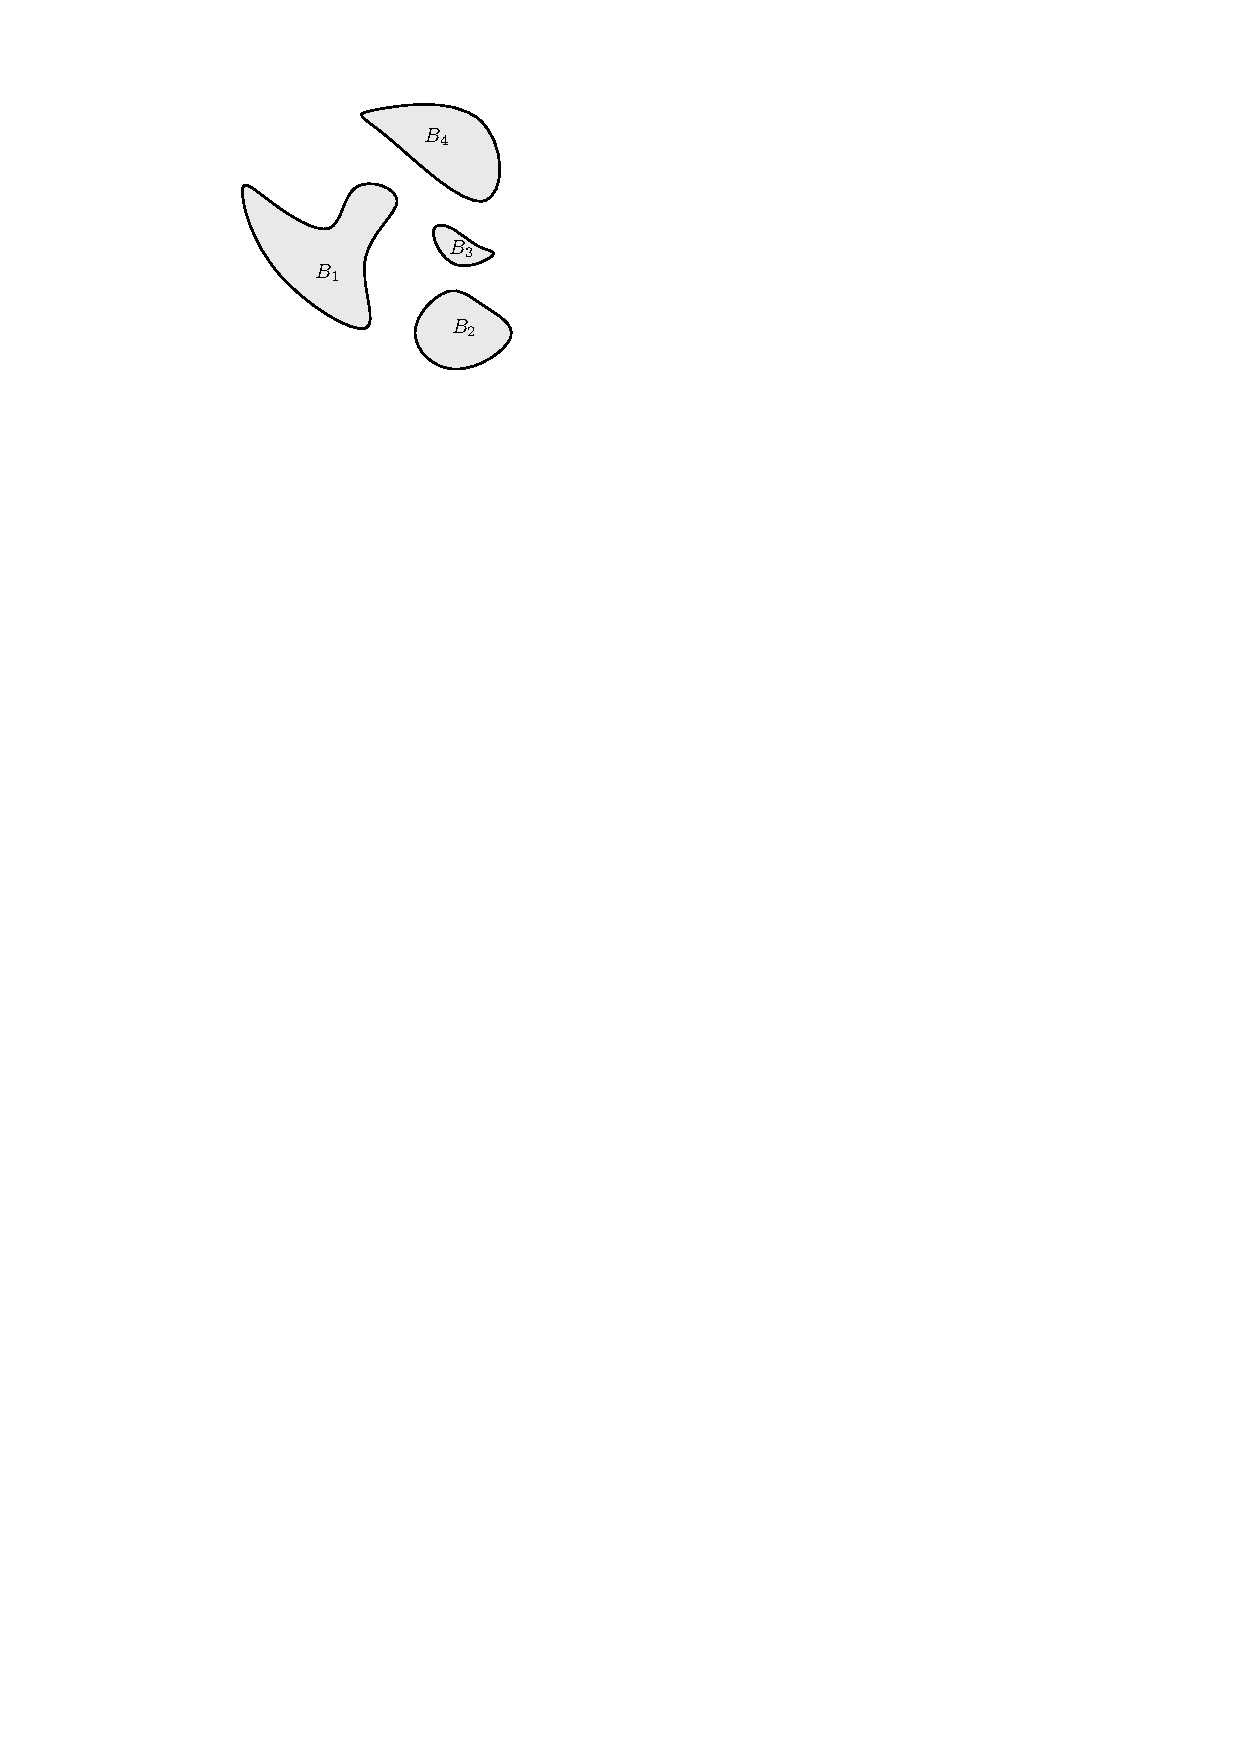
\includegraphics{ch02-bc-dimenze.pdf}
        \caption{Množina $B=\bigcup_{i=1}^4 B_i$}
        \label{subfig:bc-dimenze-pokryvana-mnozina}
    \end{subfigure}
    \qquad
    \begin{subfigure}{0.4\textwidth}
        \centering
        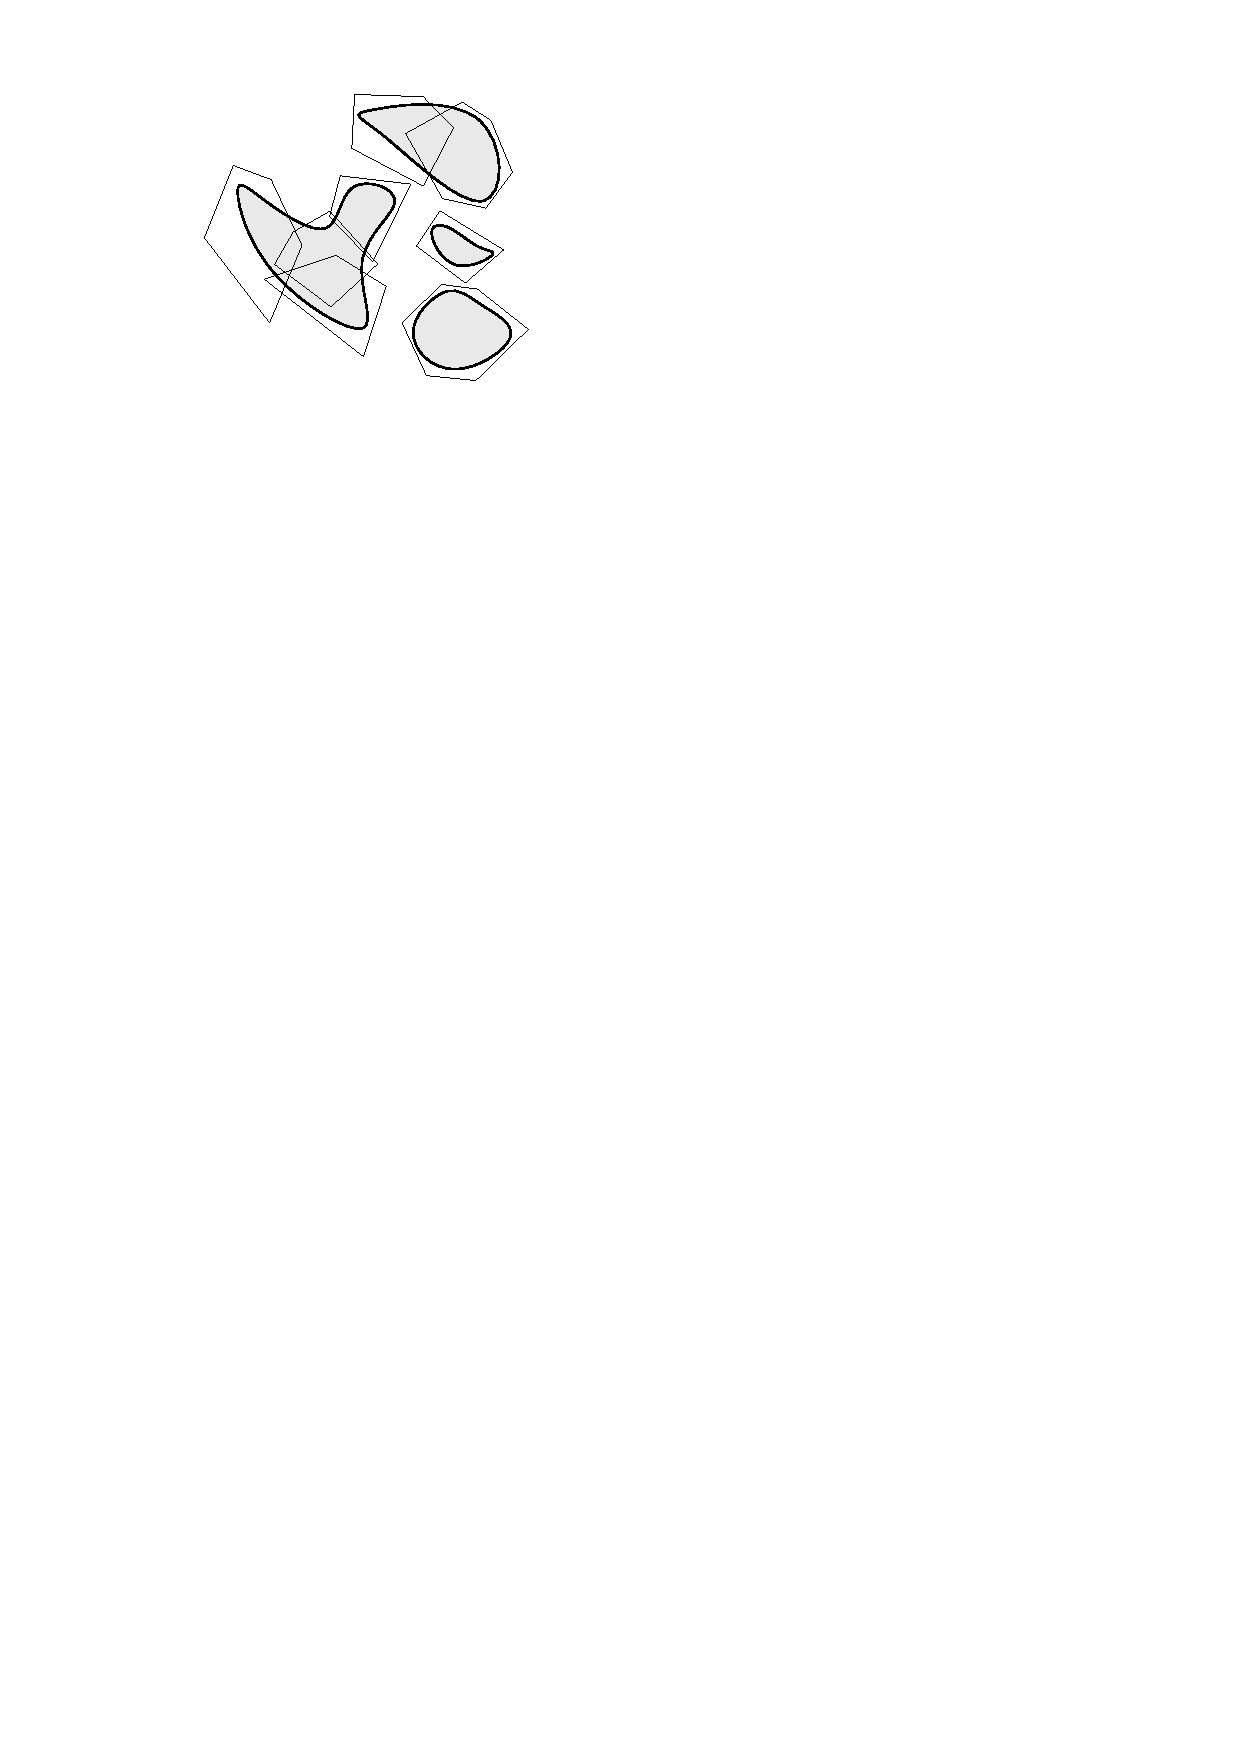
\includegraphics{ch02-bc-dimenze-delta-pokryti.pdf}
        \caption{$\delta$-pokrytí množiny $B$ (viz definice~\ref{def:box-counting-dimenze})}
        \label{subfig:bc-dimenze-delta-pokryti}
    \end{subfigure}
    \qquad
    \begin{subfigure}{0.4\textwidth}
        \centering
        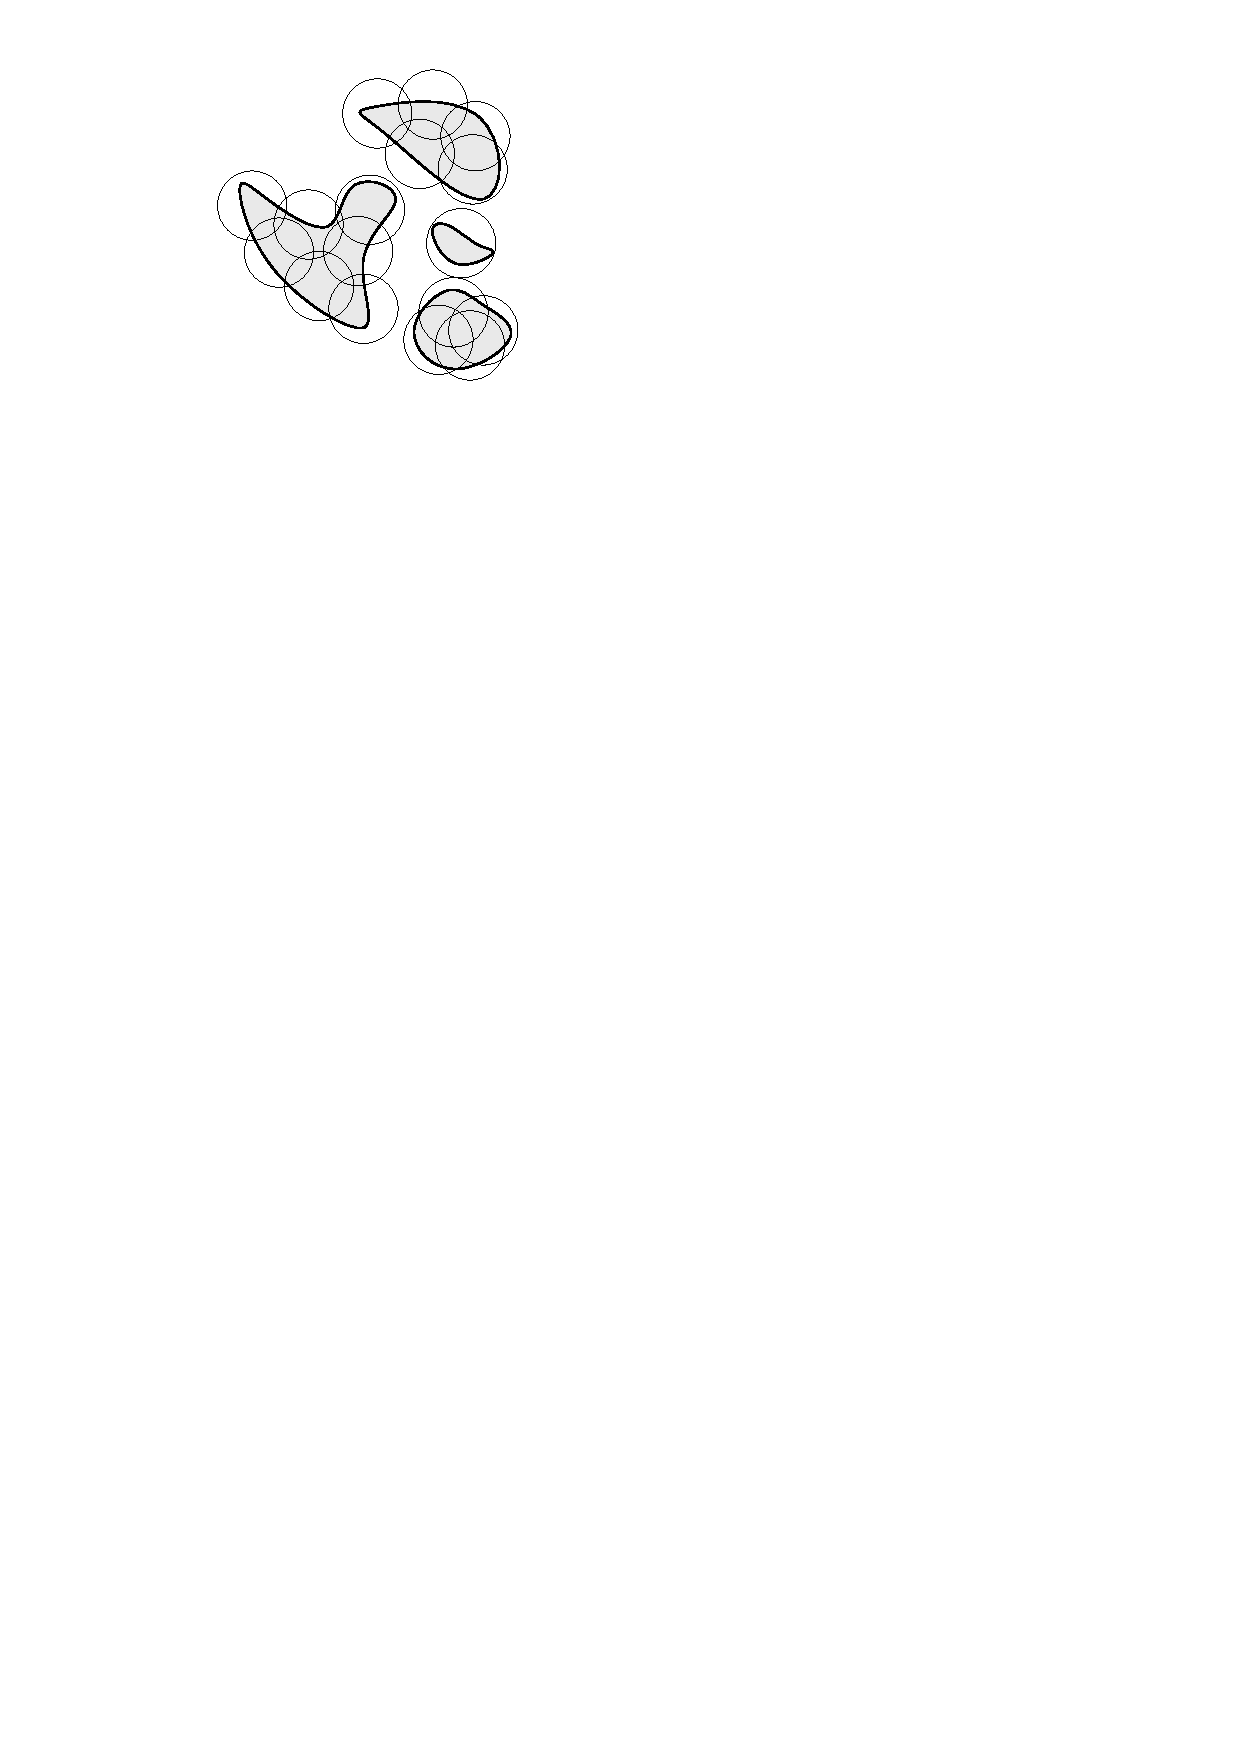
\includegraphics{ch02-bc-dimenze-pokryti-uz-koule.pdf}
        \caption{Pokrytí uzavřenými koulemi (viz bod~\ref{thm:pokryti-delta-uz-koulemi})}
        \label{subfig:bc-dimenze-uz-koule}
    \end{subfigure}
    \qquad
    \begin{subfigure}{0.4\textwidth}
        \centering
        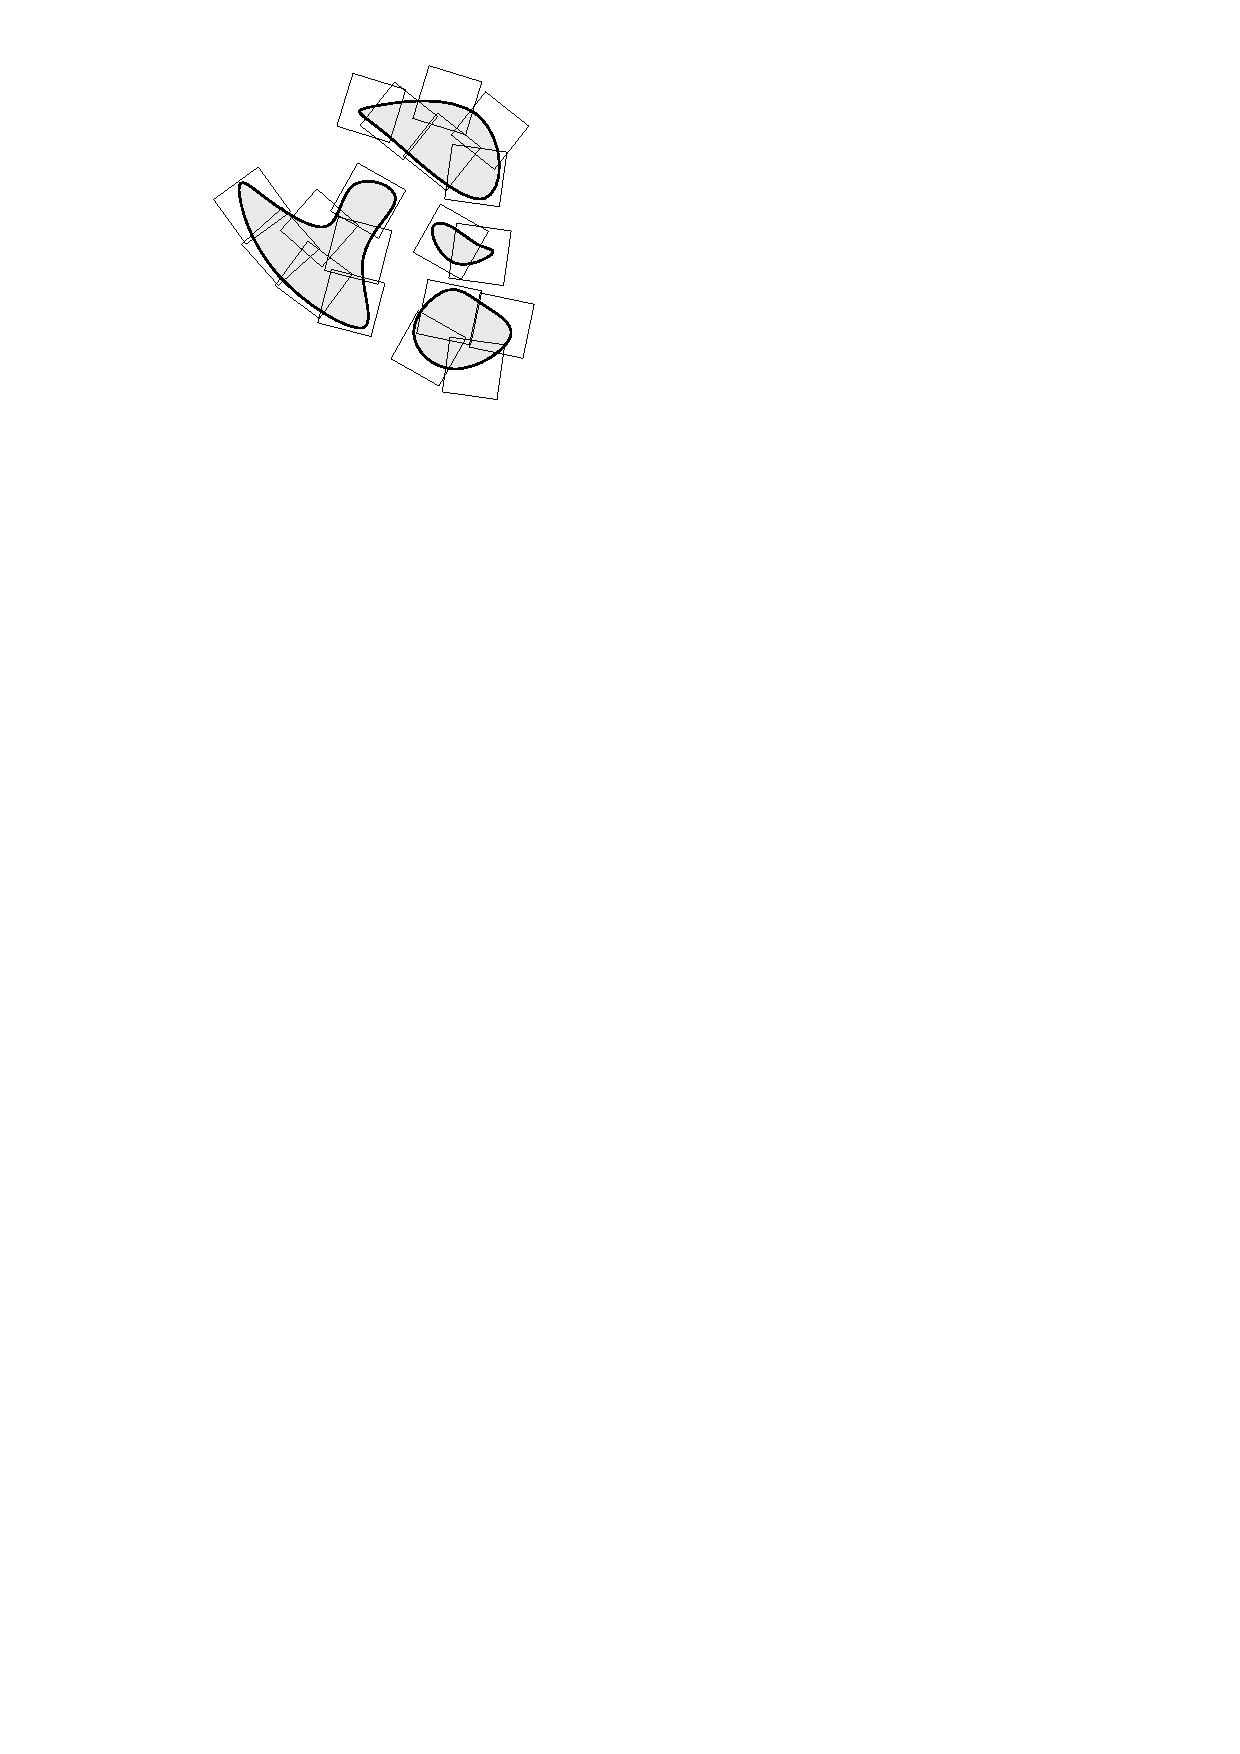
\includegraphics{ch02-bc-dimenze-pokryti-kvadry.pdf}
        \caption{Pokrytí pomocí kvádrů (viz bod~\ref{thm:pokryti-delta-kvadry})}
        \label{subfig:bc-dimenze-kvadry}
    \end{subfigure}
    \qquad
    \begin{subfigure}{0.4\textwidth}
        \centering
        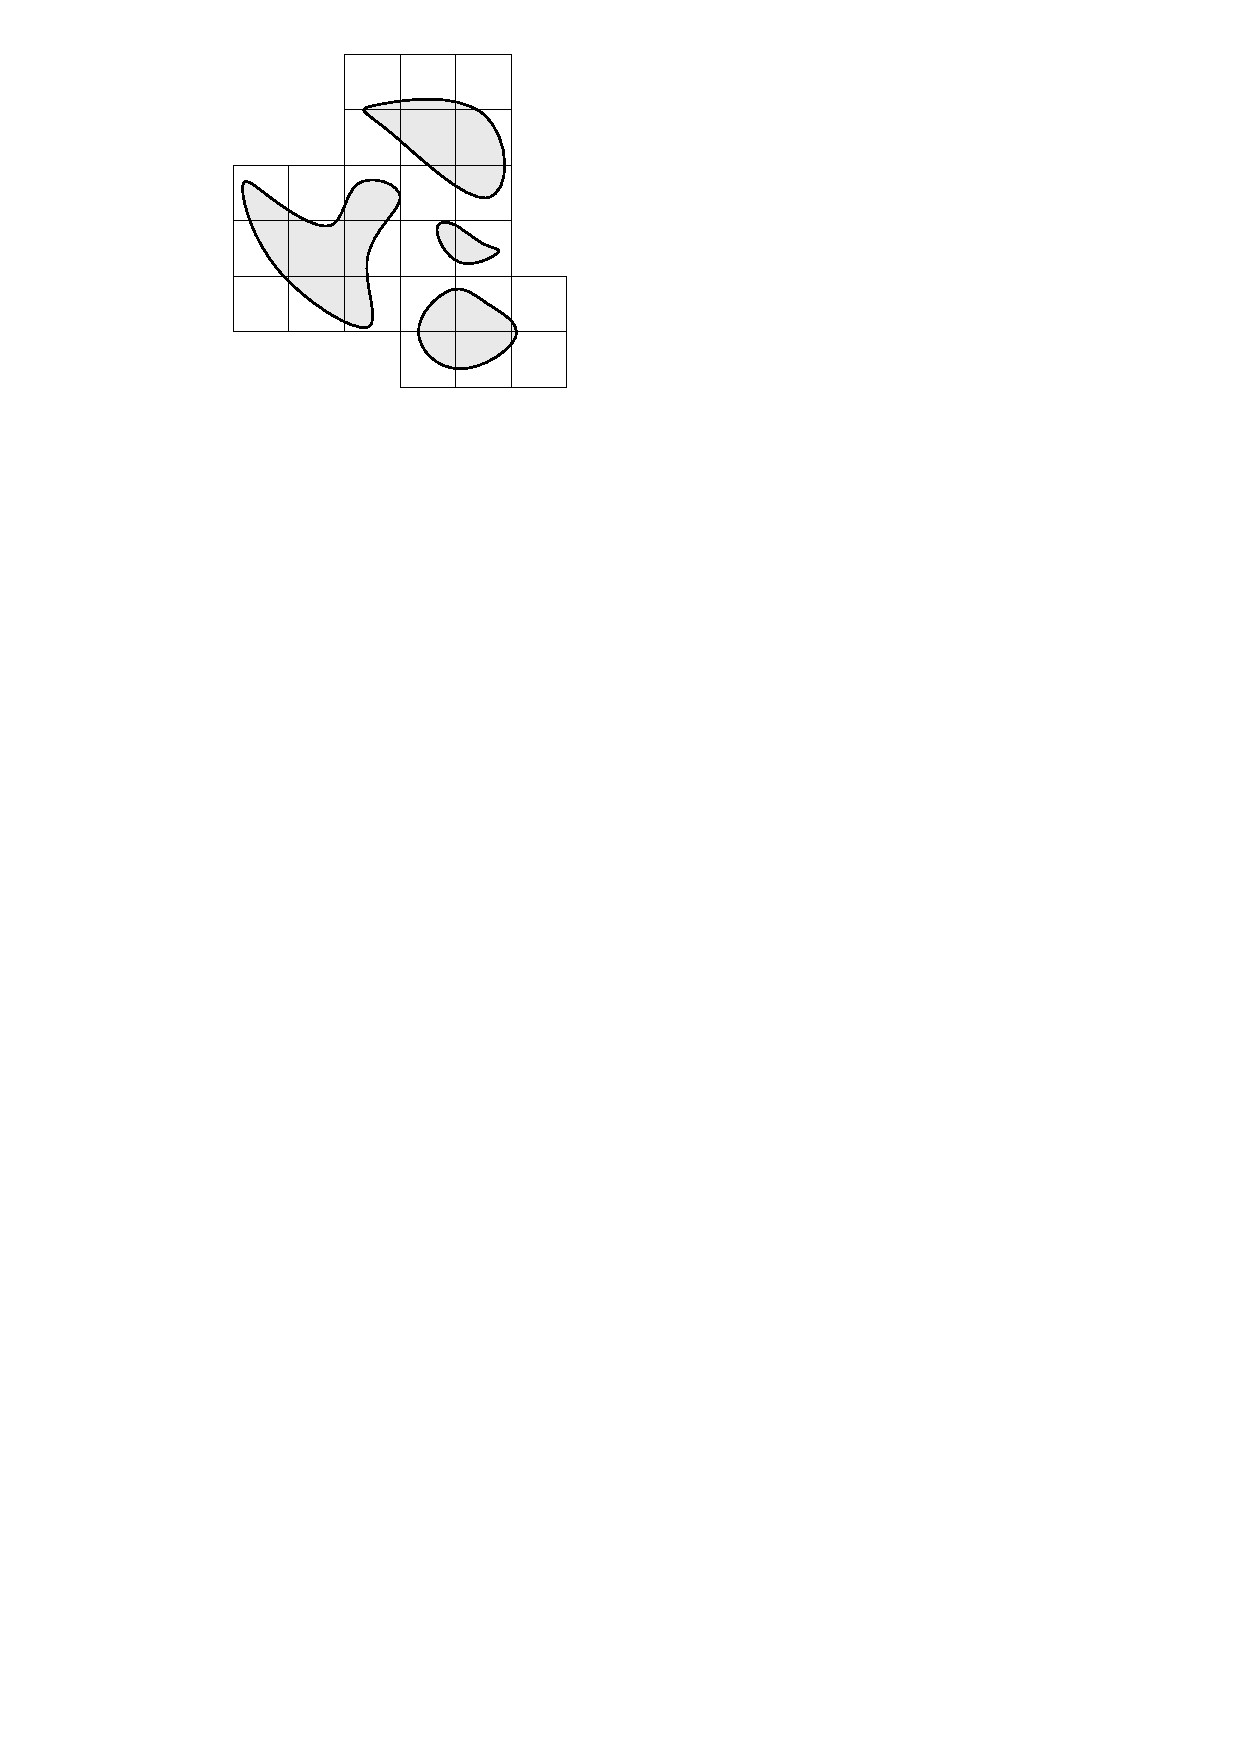
\includegraphics{ch02-bc-dimenze-pokryti-delta-sit.pdf}
        \caption{$\delta$-mříž (viz bod~\ref{thm:pokryti-delta-sit})}
        \label{subfig:bc-dimenze-delta-sit}
    \end{subfigure}
    \qquad
    \begin{subfigure}{0.4\textwidth}
        \centering
        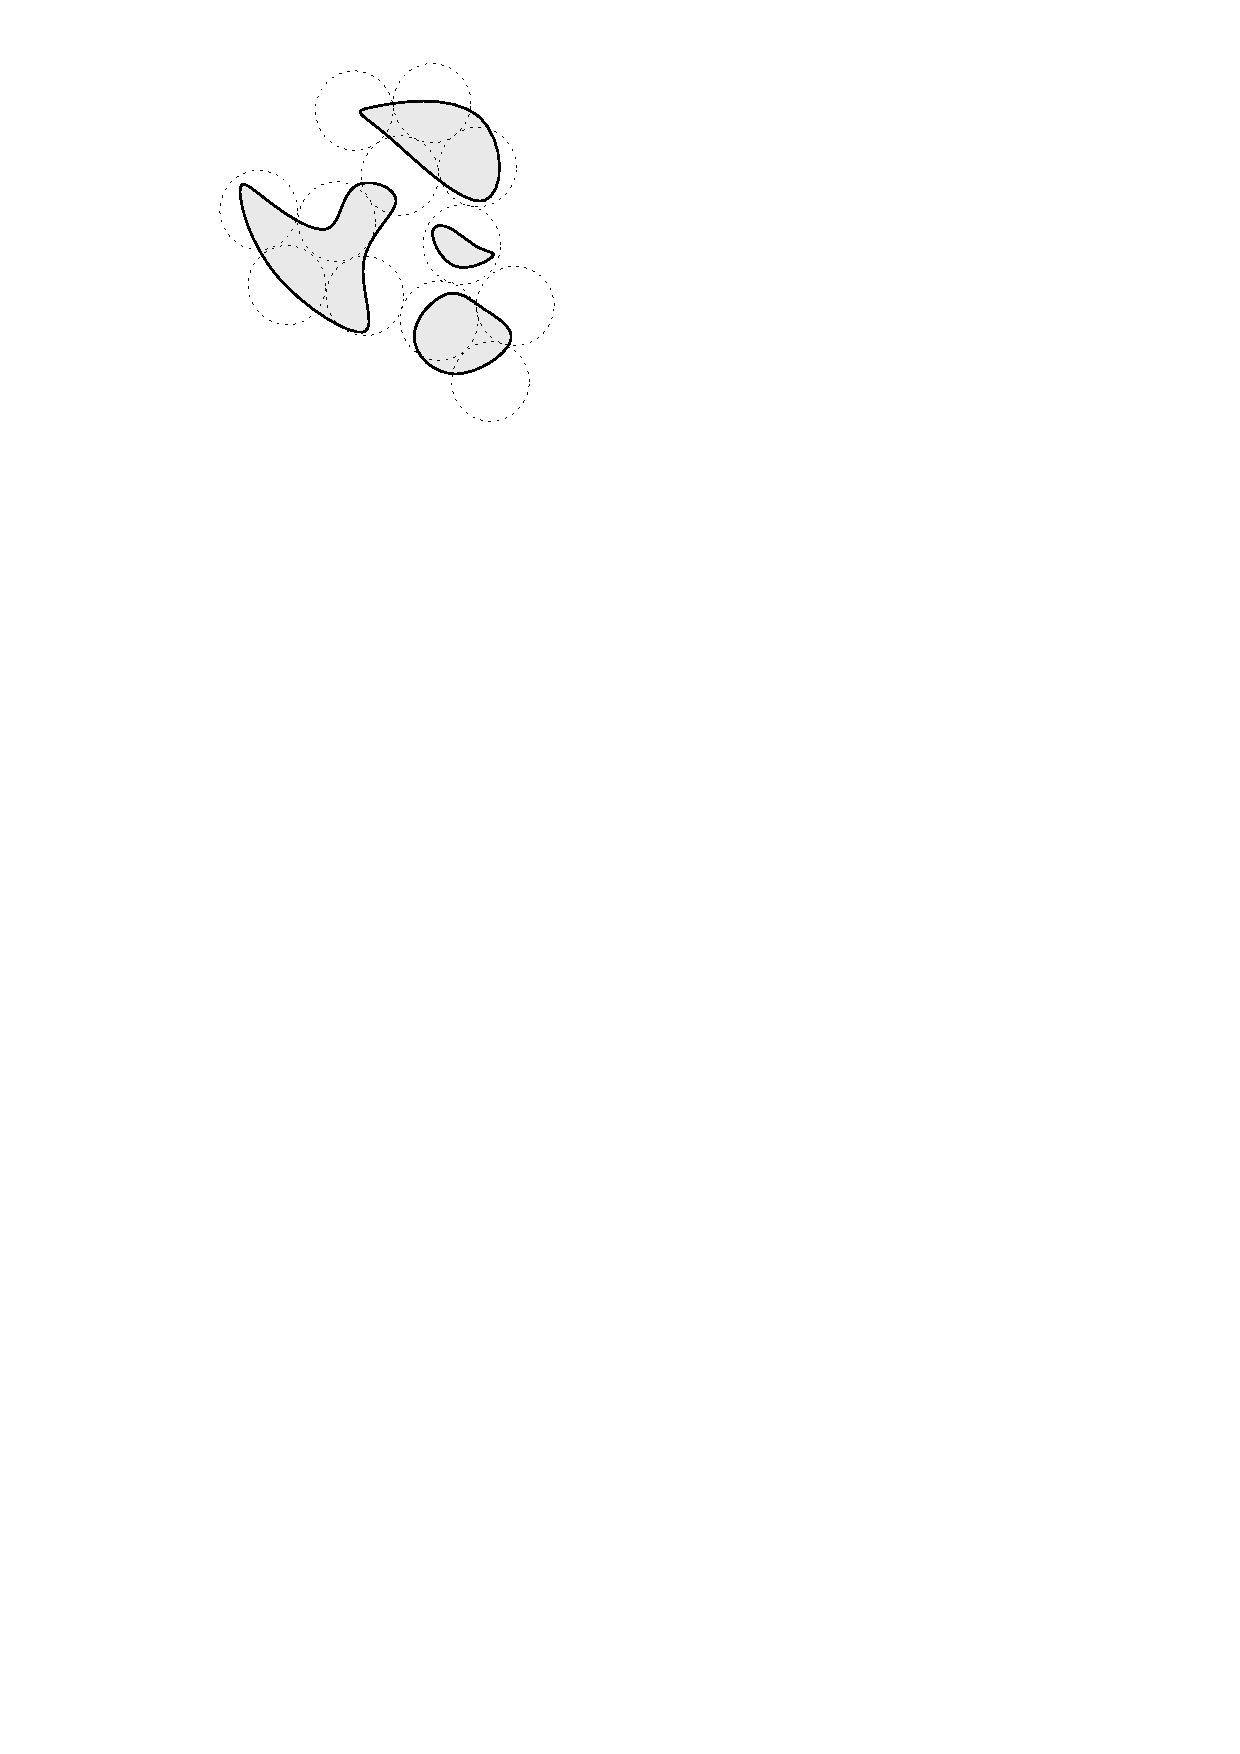
\includegraphics{ch02-bc-dimenze-pokryti-ot-koule.pdf}
        \caption{Pokrytí otevřenými po dvou disjunktními koulemi (viz bod~\ref{thm:pokryti-delta-dis-ot-koulemi})}
        \label{subfig:bc-dimenze-ot-koule}
    \end{subfigure}
    \caption[Ilustrace věty~\ref{thm:ekvivalentni-def-box-counting-dimenze}]{Ilustrace věty~\ref{thm:ekvivalentni-def-box-counting-dimenze} (Inspirováno \citep[str. 29]{Falconer2014})}
    \label{fig:ilustrace-definic-bc-dimenze}
\end{figure}

Zároveň body~\ref{thm:pokryti-delta-kvadry} a~\ref{thm:pokryti-delta-sit} nám dávají dobré opodstatnění názvu tohoto typu dimenze,~neboť v~podstatě zkoumáme pokrývání daného obrazce "kostkami". Při aproximacích box-counting dimenze obrazce $F\subset\R^2$ tak lze pracovat s~mřížkou čtverců o~libovolné straně $\delta>0$,~kdy $M_\delta(F)$ stanovíme jako počet čtverců,~které se překrývají se zkoumaným obrazcem $F$. Když se tedy zpět vrátíme k~otázce rozebírané v~úvodu tohoto textu týkající se délky pobřeží (viz kapitola~\ref{chapter:uvod_do_fraktalu}),~lze jeho "fráktálnost" do jisté míry vyjádřit právě popsaným způsobem (viz obrázek~\ref{fig:aproximace-delky-pobrezi-vb}).
\begin{figure}
    \centering
    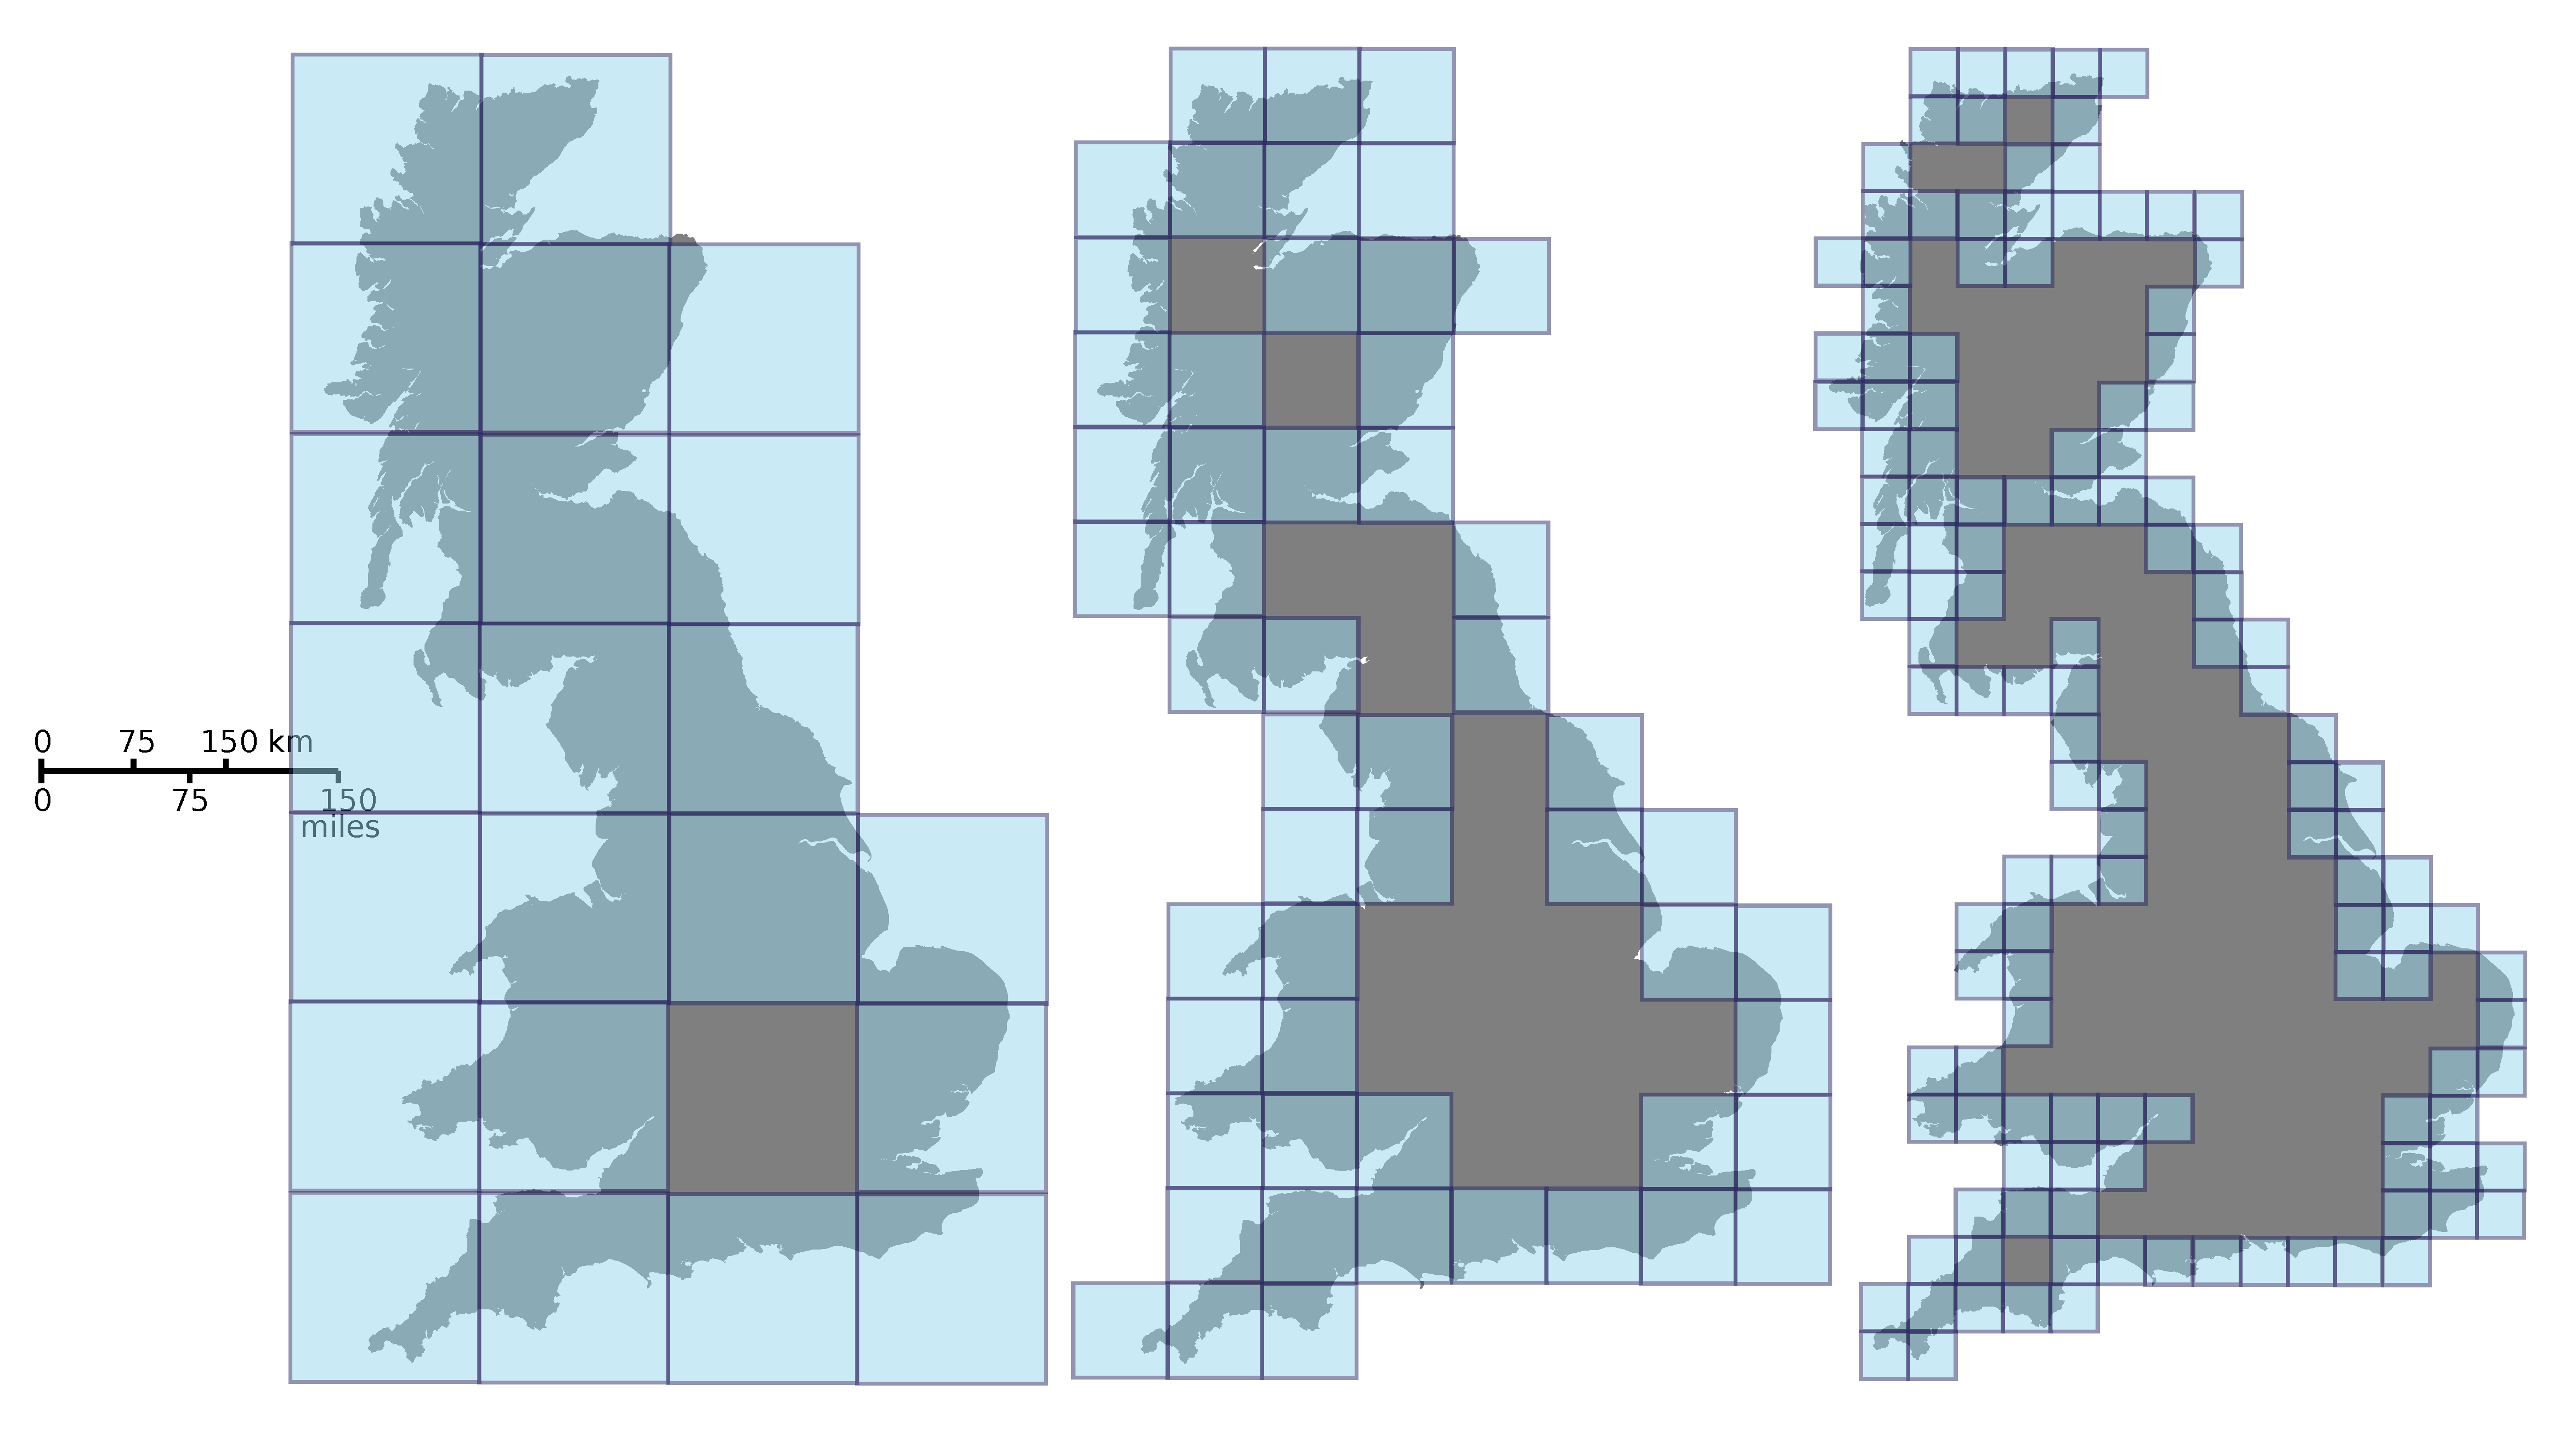
\includegraphics[width=\textwidth]{Great_Britain_Box.pdf}
    \caption[Aproximace box-counting dimenze pobřeží Velké Británie]{Aproximace box-counting dimenze pobřeží Velké Británie (Převzato z~Wikipedia Commons)\footnotemark}
    \label{fig:aproximace-delky-pobrezi-vb}
\end{figure}
Nyní se opět vrátíme k~fraktálům\footnotetext{Viz též \url{https://en.wikipedia.org/wiki/Minkowski\%E2\%80\%93Bouligand\_dimension}.} a~výpočtům jejich dimenze,~čemuž jsme se věnovali již v~sekci~\ref{sec:fraktalni_dimenze} kapitoly~\ref{chapter:uvod_do_fraktalu},~konkrétně~\ref{subsec:dimenze-fraktalu}. Tentokrát však budeme postupovat přímo podle definice box-counting dimenze~\ref{def:box-counting-dimenze},~tedy budeme zvlášť zkoumat horní a~dolní box-counting dimenzi.
\begin{example}[Cantorovo diskontinuum]\label{ex:cantorovo-diskontinuum}
    Formálně můžeme popsat Cantorovo diskontinuum $C$ jako průnik množin $C_k$ pro $k=0,1,2,\ldots$,~přičemž
    \[C_k=\bigcup _{j=0}^{3^{k-1}-1}\left(\left\langle{\frac {3j+0}{3^{k}}},{\frac {3j+1}{3^{k}}}\right\rangle\cup \left\langle{\frac {3j+2}{3^{k}}},{\frac {3j+3}{3^{k}}}\right\rangle\right).\]
    $C_k$ tedy reprezentuje $k$-tou iteraci a~$C=\bigcap_{k=0}^\infty C_k$. Již jsme měli možnost se přesvědčit,~že tento fraktál má box-counting dimenzi $\ln{2}/\ln{3}$. Zkusme nyní výpočet zopakovat,~avšak vzlášť vypočítáme $\lowerdimB{C}$ a~$\upperdimB{C}$ podíváme se,~zda se shodují.

    Jako první provedeme horní odhad. Je potřeba zvolit $\delta$ a~na jeho základě dopočítat $N_\delta(C)$. V~$k$-té iteraci,~kde $k=0,1,2,\ldots$,~bude obecně $2^k$ intervalů,~každý o~délce $(1/3)^k$,~tedy pokud zvolíme $3^{-k}<\delta\leqslant 3^{-k+1}$,~pak intervaly o~délce nejvýše $\delta$ (viz věta~\ref{thm:ekvivalentni-def-box-counting-dimenze},~bod~\ref{thm:pokryti-delta-uz-koulemi}) tvoří $\delta$ pokrytí,~přičemž $N_\delta(C)\leqslant 2^k$. Tedy celkově pro $\delta$-pokrytí všech intervalů bude potřeba nejvýše $N_\delta(C)\leqslant 2^k$ intervalů $I_1,I_2,\ldots,I_{N_\delta(C)}$ o~průměru $3^{-k}<\diam{F_i}\leqslant 3^{-k+1}$ pro každé $i$. Z~toho dostáváme
    \[\upperdimB{C}=\limsup_{\delta\to 0}\dfrac{\ln{N_\delta(C)}}{-\ln{\delta}}\leqslant\limsup_{k\to\infty}\dfrac{\ln{2^k}}{-\ln{3^{-k+1}}}=\limsup_{k\to\infty}\dfrac{k\ln{2}}{(k-1)\ln{3}}=\dfrac{\ln{2}}{\ln{3}}.\]
    Naopak pokud uvážíme intervaly délky $3^{-k-1}\leqslant\delta<3^{-k}$,~pak každý z~nich má neprázdný průnik s~maximálně jedním intervalem $k$-té iterace $C$. Těch je,~jak již víme,~$2^k$,~tedy intervalů $I_1,I_2,\ldots,I_{N_\delta(C)}$ bude nejméně $2^k$ pro pokrytí $C$,~tzn. $N_\delta(C)\geqslant 2^k$. Tím dostáváme dolní odhad:
    \[\lowerdimB{C}=\liminf_{\delta\to 0}\dfrac{\ln{N_\delta(C)}}{-\ln{\delta}}\geqslant\liminf_{\delta\to 0}\dfrac{\ln{2^k}}{-\ln{3^{-k-1}}}=\liminf_{\delta\to 0}\dfrac{k\ln{2}}{(k+1)\ln{3}}=\dfrac{\ln{2}}{\ln{3}}.\]

    Protože $\lowerdimB{C}=\upperdimB{C}=\ln{2}/\ln{3}$,~tak box-counting dimenze Cantorova diskontinua je $\dimB{C}=\ln{2}/\ln{3}$. (Převzato z~\citep[str. 32]{Falconer2014})
\end{example}
Podobně bychom postupovali pro rovinné obrazce.
\begin{example}[Kochova křivka]\label{ex:kochova-krivka}
    Zde se zatím s~formální definicí nebudeme zatěžovat. Opět ukážene horní a~dolní odhad zvlášť. Kochovu křivku si označíme $K$.

    Obecně $k$-tá iterace Kochovy křivky bude obsahovat $4^n$ úseček,~každá o~délce $(1/3)^k$. Podobně jako v~předchozím příkladu~\ref{ex:cantorovo-diskontinuum} zvolíme $3^{-k}<\delta\leqslant 3^{-k+1}$. Pokud si pro pokrytí zvolíme uzavřené koule
    \[K_\delta^1(x_1),K_\delta^2(x_2),\ldots,K_\delta^{M_\delta(K)}(x_{M_\delta(K)}),\;\text{kde}\;x_1,x_2,\ldots,x_{M_\delta(K)}\in\R^2\]
    pak $M_\delta(K)\leqslant 4^k$. Tedy
    \[\upperdimB{K}=\limsup_{\delta\to 0}\dfrac{\ln{M_\delta(K)}}{-\ln{K}}\leqslant\limsup_{k\to\infty}\dfrac{\ln{4^k}}{-\ln{3^{-k+1}}}=\limsup_{k\to\infty}\dfrac{k\ln{4}}{(k-1)\ln{3}}=\dfrac{\ln{4}}{\ln{3}}.\]

    Podobně pro dolní odhad uvážíme $3^{-k-1}\leqslant\delta<3^{-k}$. Vezmeme-li uzavřené koule $K_\delta^1(x_1),K_\delta^2(x_2),\ldots,K_\delta^{M_\delta(K)}(x_{M_\delta(K)})$,~pak žádný nemůže mít neprázdný průnik s~více než čtyřmi úsečkami,~tedy pro jejich pokrytí je zapotřebí alespoň $M_\delta(K)\geqslant 4^k/4=4^{k-1}$,~čímž dostáváme
    \[\lowerdimB{K}=\liminf_{\delta\to 0}\dfrac{\ln{M_\delta(K)}}{-\ln{K}}\geqslant\liminf_{k\to\infty}\dfrac{\ln{4^{k-1}}}{-\ln{3^{-k-1}}}=\liminf_{k\to\infty}\dfrac{(k-1)\ln{4}}{(k+1)\ln{3}}=\dfrac{\ln{4}}{\ln{3}}.\]
    Tzn.~$\dimB{K}=\ln{4}/\ln{3}$.
\end{example}
\begin{remark}
    Obecně množina $F$ skládající se z~$m$ disjunktních kopií sebe samotné,~kde každá z~nich je $r$-krát menší,~má dimenzi $\dimB{F}=\ln{m}/\ln{r}$.
\end{remark}
Nyní se podíváme ještě na jedno možné pojetí box-counting dimenze. Připomeňme,~že $\delta$-okolím množiny $F$ v~metrickém prostoru $(X,\varrho)$ rozumíme
\[(F)_\delta=\set{x\in X\mid\exists y\in X: \varrho(x,y)<\delta}.\]
Budeme nyní sledovat,~jak "rychle" se mění objem $(F)_\delta$ pro $\delta\to 0$. A~se zmínkou objemu nám zde do hry opět vstupuje Lebesgueova míra $\lebesguemeasure{n}$,~o níž jsme si povídali v~sekci~\ref{sec:lebesgueova-mira}. Podívejme se nejdříve na několik příkladů.
\begin{itemize}
    \item Pro konečnou množinu $F=\set{x_1,x_2,\ldots,x_n}$ je
    \[\lebesguemeasure{3}((F)_\delta)\leqslant n\cdot\dfrac{4}{3}\pi\delta^3.\]
    Pro $\delta\leqslant1/2\min\set{\varrho(x,y)\mid x,y\in F}$ nastává rovnost.
    \item Pro úsečku $u\subset\R^3$ o~délce $\ell$ lze objem jejího $\delta$-okolí stanovit jako
    \[\lebesguemeasure{3}((u)_\delta)=\dfrac{4}{3}\pi \delta^3+\pi\delta^2\ell.\]
    Pokud však uvážíme $\delta$ dostatečně malé,~lze první člen zanedbat a~psát
    \[\lebesguemeasure{3}((u)_\delta)\approx\pi\ell\delta^2.\]
    \item V~případě neprázdného kvádru
    \[I=\set{(x,y,0)\mid x\in\langle a_1,b_1\rangle\,,\,y\in\langle a_2,b_2\rangle}\]
    je
    \begin{align*}
        \lebesguemeasure{3}(I_\delta)&=2(b_1-a_1)(a_2-b_2)\delta+2(b_1-a_1)\pi\delta^2+2(b_2-a_2)\pi\delta^2+\dfrac{4}{3}\pi\delta^3\\
        &\approx 2(b_1-a_1)(a_2-b_2)\delta
    \end{align*}
    \item Pro kouli $B_r(x)\subset\R^3$,~kde $x\in\R^3$ a~$r>0$ je objem
    \[\lebesguemeasure{3}((B_r(x))_\delta)=\dfrac{4}{3}\pi (r+\delta)^3=\dfrac{4}{3}\pi r^3+4\pi r^2\delta+4\pi r\delta^2+\dfrac{4}{3}\pi\delta^3\approx\dfrac{4}{3}\pi r^3.\]
    Změna objemu je v~tomto případě vzhledem k~původnímu objemu zanedbatelná.
\end{itemize}
Výsledky si srovnejme v~tabulce~\ref{table:odhady-lambda_3}.
\begin{table}[h]
    \centering
    \begin{tabular}{r|D{=}{=}{-1}}
    Útvar $F$                               & \multicolumn{1}{c}{$\lebesguemeasure{3}((F)_\delta)$}       \\\hline
    Konečná množina $\set{x_1,\ldots,x_n}$     & \frac{4n}{3}\pi\delta^3=c_1\delta^3   \\
    Úsečka $u$                             & \pi\ell\delta^2=c_2\delta^2           \\
    Kvádr $I$                              & 2(b_1-a_1)(a_2-b_2)\delta=c_3\delta^1 \\
    Koule $B_\delta(x)$                    & \frac{4}{3}\pi r^3=c_4\delta^0      
    \end{tabular}
    \caption{Odhady $\lebesguemeasure{3}$ pro vybrané útvary}
    \label{table:odhady-lambda_3}
\end{table}
Můžeme si všimnout,~že v~každém případě odhad objemu vychází $\lebesguemeasure{3}((F)_\delta)\approx c\delta^{3-s}$,~kde $c>0$ je závislé na původní míře $F$ a~$s$ udává dimenzi. Obecněji pro množinu $F\subseteq\R^n$ bychom došli k~$\lebesguemeasure{n}((F)_\delta)\approx c\delta^{n-s}$. Nyní,~podobně jako v~úvodu této sekce,~zkusme opět vyjádřit $s$:
\begin{align*}
    \ln{\lebesguemeasure{n}((F)_\delta)}&\approx\ln{c}+(n-s)\ln{\delta}\\
    s\ln{\delta}&\approx n\ln{\delta}-\ln{\lebesguemeasure{n}((F)_\delta)}+\ln{c}\\
    s&\approx n-\dfrac{\ln{\lebesguemeasure{n}((F)_\delta)}}{\ln{\delta}}+\dfrac{\ln{c}}{\ln{\delta}}.
\end{align*}
Poslední člen bude v~limitě opět nulový.

Lze ukázat,~že $s$ není v~tomto případě nic jiného,~než již námi zkoumaná\linebreak{}box-counting dimenze. To si shrneme a~dokážeme ve větě~\ref{thm:bc-dimenze-lebesgueova-mira}.
\begin{theorem}\label{thm:bc-dimenze-lebesgueova-mira}
    Nechť $F\subseteq\R^n$. Pak platí: 
    \begin{enumerate}[label=(\roman*)]
        \item $\lowerdimB{F}=n-\limsup\limits_{\delta\to 0}\dfrac{\ln{\lebesguemeasure{n}((F)_\delta)}}{\ln{\delta}}$,
        \item $\upperdimB{F}=n-\liminf\limits_{\delta\to 0}\dfrac{\ln{\lebesguemeasure{n}((F)_\delta)}}{\ln{\delta}}$.
    \end{enumerate}
\end{theorem}
\begin{proof}
    V~rámci důkazu využijeme větu~\ref{thm:ekvivalentni-def-box-counting-dimenze}.

    Mějme $F\subseteq\R^n$. Označme $v_n$ objem jednotkové koule $K_1(x)$\footnote{Objem koule v~$\R^n$ lze vyjádřit vztahem
    \[V_n(r)=\dfrac{\pi^{n/2}}{\Gamma\left(\frac{n}{2}+1\right)}r^n,\]
    kde $\Gamma$ je tzv. \emph{gamma funkce}. Se vzorcem však dále v~textu pracovat nebudeme.
    } v~$\R^n$ pro $x\in\R^n$ libovolné. Dále mějmě pokrytí
    \[\mathcal{K}=\set{K_\delta^1(x_1),K_\delta^2(x_2),\ldots,K_\delta^{M_\delta(F)}(x_{M_\delta(F)})}\]
    množiny $F$,~kde $0<\delta<1$ a~$x_j\in F$ pro každé $1\leqslant j\leqslant M_\delta(F)$,~přičemž $M_\delta(F)$ je definováno podle bodu~\ref{thm:pokryti-delta-uz-koulemi} věty~\ref{thm:ekvivalentni-def-box-counting-dimenze}. Pak lze zvolit pokrytí
    \[\mathcal{K}^\prime=\set{K_{2\delta}^1(x_1),K_{2\delta}^2(x_2),\ldots,K_{2\delta}^{M_\delta(F)}(x_{M_\delta(F)})},\]
    tzn.~$\mathcal{K}$ je zjemnění pokrytí $\mathcal{K}^\prime$. Zároveň však platí,~že $\mathcal{K}^\prime$ je i~pokrytím $(F)_\delta$. Pro libovolné $x\in (F)_\delta$ existuje totiž $y\in F$,~takové,~$\varrho(x,y)<\delta$. Tedy pro dané $y$ existuje nějaká koule $K_\ell(x_\ell)\in\mathcal{K}$,~taková,~že $y\in K_\ell(x_\ell)$,~což znamená,~že
    \[\varrho(x_\ell,y)\leqslant\varrho(x_\ell,x)+\varrho(x,y)\leqslant\delta+\delta=2\delta.\]
    Tzn.~míru $F$ lze zhora odhadnout jako
    \[\lebesguemeasure{n}((F)_\delta)\leqslant M_\delta(F)v_n(2\delta)^n.\]
    Úpravou získáme:
    \begin{align*}
        \ln{\lebesguemeasure{n}((F)_\delta)}&\leqslant n\ln{\delta}+\ln{M_\delta(F)}+\ln{2^nv_n}\\
        \dfrac{\ln{\lebesguemeasure{n}((F)_\delta)}}{-\ln\delta}&\leqslant -n+\dfrac{\ln{M_\delta(F)}}{-\ln\delta}+\dfrac{\ln{2^nv_n}}{-\ln\delta},
    \end{align*}
    tedy v~limitě
    \[\liminf_{\delta\to 0}\dfrac{\ln\lebesguemeasure{n}((F)_\delta)}{-\ln\delta}\leqslant -n+\lowerdimB{F}.\]
    K~odhadu $\upperdimB{F}$ lze dospět analogicky.

    Nyní uvažujme po dvou disjunktní otevřené koule $B_\delta^j(x_j)$,~kde $x_j\in F$ pro $1\leqslant j\leqslant M_\delta(F)$. Pak součtem jejich objemů získáme
    \[M_\delta(F)v_n\delta^n\leqslant\lebesguemeasure{n}((F)_\delta).\]
    Obdobnou úpravou této nerovnosti získáme požadovanou nerovnost.
\end{proof}
Zkusme si aplikaci věty ilustrovat opět na příkladu fraktálu.
\begin{example}[Cantorovo diskontinuum potřetí]\label{ex:cantorovo-diskontinuum-potreti}
    Pro Cantorovo diskontinuum v~$k$-té iteraci,~označme $C_k$,~lze odhadnout délku $(C_k)_\delta$ pro $3^{-k-2}\leqslant\delta\leqslant 3^{-k-1}$ jako
    \[\lebesguemeasure{1}((C_k)_\delta)\geqslant 2^k(3^{-k-2}+2\delta)\leqslant2^k\cdot 3\cdot 3^{-k-2}=2^k\cdot 3^{-k-1}.\]
    Tedy podle věty~\ref{thm:bc-dimenze-lebesgueova-mira}
    \begin{align*}
        \upperdimB{C}&=n-\liminf_{\delta\to 0}\dfrac{\ln{\lebesguemeasure{1}((C)_\delta)}}{\ln{\delta}}\leqslant1-\liminf_{k\to\infty}\dfrac{\ln{2^{k}\cdot 3^{-k-1}}}{\ln{3^{-k-1}}}\\
        &=\liminf_{k\to\infty}\dfrac{k\ln{2}}{(k+1)\ln{3}}=\dfrac{\ln{2}}{\ln{3}}.
    \end{align*}

    Podobně zvolíme-li $3^{-k-1}\leqslant\delta\leqslant 3^{-k}$,~pak
    \[\lebesguemeasure{1}((C_k)_\delta)\leqslant 2^k(3^{-k}+2\delta)\leqslant2^k\cdot 3\cdot 3^{-k}=2^k\cdot 3^{-k+1}\]
    a~tedy
    \begin{align*}
        \lowerdimB{C}&=n-\limsup_{\delta\to 0}\dfrac{\ln{\lebesguemeasure{1}((C)_\delta)}}{\ln{\delta}}\geqslant 1-\limsup_{k\to\infty}\dfrac{\ln{2^{k}\cdot 3^{-k+1}}}{\ln{3^{-k+1}}}\\
        &=\limsup_{k\to\infty}\dfrac{k\ln{2}}{(k-1)\ln{3}}=\dfrac{\ln{2}}{\ln{3}}.
    \end{align*}
\end{example}

\subsection{Vlastnosti}\label{subsec:vlastnosti-bc-dimenze}

V minulé podsekci~\ref{subsec:definice-a-vypocet-bc-dimenze} jsme se bavili o~možnostech pojetí box-counting dimenze. S~tím souvisely zejména pak věty~\ref{thm:ekvivalentni-def-box-counting-dimenze} a~\ref{thm:bc-dimenze-lebesgueova-mira}. Nyní trochu blíže ještě prozkoumáme některé její vlastnosti,~na něž se podíváme ve větě~\ref{thm:vlastnosti-bc-dimenze}.
\begin{theorem}[Vlastnosti box-counting dimenze]\label{thm:vlastnosti-bc-dimenze}
    Nechť jsou dány $F,G\subseteq\R^n$.
    \begin{enumerate}[label=(\roman*)]
        \item\label{thm:monotonie-bc-dimenze} Pokud $G\subseteq F$,~pak $\lowerdimB{G}\leqslant\lowerdimB{F}$ a~$\upperdimB{G}\leqslant\upperdimB{F}$.\rightnote{monotonie}
        \item\label{thm:rozsah-hodnot-bc-dimenze} Je-li $F\neq\emptyset$ omezená,~pak $0\leqslant\lowerdimB{F}\leqslant\upperdimB{F}\leqslant n$.\rightnote{rozsah hodnot}
        \item\label{thm:stabilita-bc-dimenze} $\upperdimB(F\cup G)=\max\set{\upperdimB{F},\upperdimB{G}}$.\rightnote{stabilita}
    \end{enumerate}
\end{theorem}
\begin{proof}
    \begin{enumerate}[label=\textit{(\roman*)}]
        \item Plyne triviálně z~faktu,~že pro libovolné $\delta>0$ je $N_\delta(G)\leqslant N_\delta(F)$,~neboť každé $\delta$-pokrytí $\mathcal{F}\supset F$ je zároveň $\delta$-pokrytím $G$.
        \item První dvojice nerovností je zjevná z~definice (viz~\ref{def:box-counting-dimenze}). Pro třetí nerovnost zvolme kvádr $I$,~takový,~že $F\subset I$. Zvolíme-li $\delta>0$ a~$\delta$-mříž $\mathcal{Q}_\delta$,~pak
        \begin{align*}
            M_\delta(F)&=\left|\set{J\;\middle|\;J\cap F\neq\emptyset\;,\;J\in\mathcal{Q}_\delta}\right|\\
            &\leqslant \left|\set{J\;\middle|\;J\cap I\neq\emptyset\;,\;J\in\mathcal{Q}_\delta}\right|\\
            &=M_\delta(I)\leqslant c\delta^{-n},
        \end{align*}
        kde $c>0$. Poslední nerovnost si lze snadno rozmyslet. Tedy podle věty~\ref{thm:ekvivalentni-def-box-counting-dimenze} a~přechozího bodu~\ref{thm:monotonie-bc-dimenze} máme
        \[\upperdimB{F}\leqslant\upperdimB{I}=\limsup_{\delta\to 0}\dfrac{\ln{N_\delta(I)}}{-\ln{\delta}}\leqslant\limsup_{\delta\to 0}\dfrac{\ln{c\delta^{-n}}}{-\ln{\delta}}=n.\]
        \item Pro $\delta>0$ volme $\delta$-pokrytí $\mathcal{F}\supset F$ a~$\mathcal{G}\supset G$. Je celkem zjevné,~že $N_\delta(F\cup G)\leqslant N_\delta(F)+N_\delta(G)$,~neboli
        \begin{align*}
            \ln(N_\delta(F)+N_\delta(G))&\leqslant \ln\left(2\max\set{N_\delta(F),N_\delta(G)}\right)\\
            &=\ln{2}+\ln\left(\max\set{N_\delta(F),N_\delta(G)}\right).
        \end{align*}
        Tedy
        \begin{align*}
            \upperdimB(F\cup G)&\leqslant\limsup_{\delta\to 0}\left(\dfrac{\ln{2}}{-\ln{\delta}}+\dfrac{\ln\left(\max\set{N_\delta(F),N_\delta(G)}\right)}{-\ln{\delta}}\right)\\
            &\leqslant\limsup_{\delta\to 0}\dfrac{\ln\left(\max\set{N_\delta(F),N_\delta(G)}\right)}{-\ln{\delta}}\\
            &=\limsup_{\delta\to 0}\left(\max\set{\dfrac{\ln{N_\delta(F)}}{-\ln{\delta}},\dfrac{\ln{N_\delta(G)}}{-\ln{\delta}}}\right)\\
            &\leqslant\max\set{\limsup_{\delta\to 0}\dfrac{\ln{N_\delta(F)}}{-\ln{\delta}},\limsup_{\delta\to 0}\dfrac{\ln{N_\delta(G)}}{-\ln{\delta}}}\\
            &=\max\set{\upperdimB{F},\upperdimB{G}}.
        \end{align*}
        Opačná nerovnost plyne z~faktu,~že $F\subset F\cup G$ a~$G\subset F\cup G$,~tedy
        \[\upperdimB(F\cup G)\geqslant\upperdimB{F}\;\text{a}\;\upperdimB(F\cup G)\geqslant\upperdimB{G}\]
        podle bodu~\ref{thm:monotonie-bc-dimenze},~neboli
        \[\upperdimB(F\cup G)=\max\set{\upperdimB{F},\upperdimB{G}}.\]
    \end{enumerate}
\end{proof}
(Převzato a~upraveno z~\citep[str. 35]{Falconer2014}.)

Poslední bod~\ref{thm:stabilita-bc-dimenze} tvrzení~\ref{thm:vlastnosti-bc-dimenze} lze pochopitelně rozšířit indukcí. Čtenář se sám může přesvědčit,~že se jedná o~relativně jednoduché cvičení.
\begin{corollary}\label{cor:stabilita-bc-dimenze-obecne}
    Pro $F_1,F_2,\ldots,F_m\subseteq\R^n$ platí:
    \[\upperdimB\left(\bigcup_{i=1}^m F_i\right)=\max\set{\upperdimB{F_j}\mid 1\leqslant j\leqslant m}.\]
\end{corollary}
\begin{proof}
    Pro $m=1$ a~$m=2$ víme,~že tvrzení platí. Pro $m+1$ lze psát:
    \begin{align*}
        \upperdimB\left(\bigcup_{i=1}^{m+1}F_i\right)&=\upperdimB\left(\left(\bigcup_{i=1}^{m}F_i\right)\cup F_{m+1}\right)\\
        &=\max\set{\upperdimB\left(\bigcup_{i=1}^{m+1}F_i\right),\upperdimB{F_{m+1}}}\\
        &\stackrel{\text{I.P.}}{=}\max\set{\max\set{\upperdimB{F_i}\mid 1\leqslant i\leqslant m},\upperdimB{F_{m+1}}}\\
        &=\max\set{\upperdimB{F_j}\mid 1\leqslant j\leqslant m+1}.
    \end{align*}
\end{proof}

Jako poslední se ještě nabízí otázka,~jak se bude dimenze $\dimB$ chovat vůči zobrazením. V~tomto kontextu pro nás budou relevantní především \emph{lipschitzovská}\index{zobrazení!lipschitzovské}\index{lipschitzovské zobrazení} a~\emph{bilipschitzovská zobrazení}\index{zobrazení!bilipschitzovské}\index{bilipschitzovské zobrazení}. Připomeňme,~že lipschitzovské zobrazení je takové zobrazení $\mapping{f}{X}{Y}$ mezi metrickými prostory $(X,\varrho_1)$ a~$(Y,\varrho_2)$,~že existuje konstanta $K>0$,~taková,~že pro každé $x,y\in X$ platí
\[\varrho_2(f(x),f(y))\leqslant K\varrho_1(x,y).\]
Pokud navíc platí,~že existují konstanty $K_1,K_2>0$,~takové,~že platí
\[K_1\varrho_1(x,y)\leqslant\varrho_2(f(x),f(y))\leqslant K_2\varrho_1(x,y),\]
pak $f$ nazýváme bilipschitzovské.

Než se však podíváme na samotný vztah box-counting dimenze a~lipschitzovských,~resp. bilipschitzovských zobrazení,~dokážeme si jedno jednoduché\linebreak{}lemma,~které později využijeme.
\begin{lemma}\label{lem:lipschitzovska-zobrazeni-a-bijekce}
    Nechť $(X,\varrho_1),(Y,\varrho_2)$ jsou metrické prostory a~zobrazení $\mapping{f}{X}{Y}$ je bilipschitzovské. Pak $\mapping{f}{X}{f(X)}$ je bijekce.
\end{lemma}
\begin{proof}
    Podle předpokladu je $f$ bilipschitzovské zobrazení,~tedy existují pro konstanty $K_1,K_2>0$,~takové,~že
    \[K_1\varrho_1(x,y)\leqslant\varrho_2(f(x),f(y))\leqslant K_2\varrho_1(x,y),\;x,y\in X.\]
    Surjektivita zobrazení $f$ je zřejmá z~její definice. Pro spor předpokládejme,~že $f$ není injektivní,~tedy existují $x,y\in X$,~taková,~že $x\neq y$ a~$f(x)=f(y)$. Pak
    \[0<K_1\varrho_1(x,y)\leqslant\varrho_2(f(x),f(y))=0,\]
    což je spor.
\end{proof}

V našem případě se nyní dále omezíme,~stejně jako předtím,~pouze na prostor $\R^n$.

\begin{theorem}\label{thm:bc-dimenze-bi-lipschitzovska-zobrazeni}
    Nechť jsou dány metrické prostory $(\R^n,\varrho_n)$ a~$(\R^m,\varrho_m)$,~$F\subseteq\R^n$ a~zobrazení $\mapping{f}{F}{\R^m}$. Platí:
    \begin{enumerate}[label=(\roman*)]
        \item\label{thm:bc-dimenze-lipschitz} Je-li $f$ lipschitzovské,~pak
        \[\lowerdimB{f(F)}\leqslant\lowerdimB{F}\;\text{a}\;\upperdimB{f(F)}\leqslant\upperdimB{F}.\]
        \item\label{thm:bc-dimenze-bilipschitz} Je-li $f$ bilipschitzovské,~pak
        \[\lowerdimB{f(F)}=\lowerdimB{F}\;\text{a}\;\upperdimB{f(F)}=\upperdimB{F}.\]
    \end{enumerate}
\end{theorem}
\begin{proof}
    Máme tedy metrické prostory $(\R^n,\varrho_n)$,~$(\R^m,\varrho_m)$,~zobrazení $\mapping{f}{F}{\R^m}$ a~$F\subseteq\R^n$.
    \begin{enumerate}[label=\textit{(\roman*)}]
        \item Jako první si všimneme,~že je-li $\mathcal{F}=\set{F_1,F_2,\ldots}$ $\delta$-pokrytí množiny $F$,~kde $\delta>0$,~pak je jím i~systém
        \[\mathcal{F}^\prime=\set{F\cap F_1,F\cap F_2,\ldots}.\]
        Podle předpokladu je $f$ lipschitzovské,~tzn. pro každé $x,y\in\R^n$ je
        \[\varrho_m(f(x),f(y))\leqslant K\varrho_n(x,y),\;K>0.\]
        Speciálně tak platí i~$\diam(f(F\cap F_i))\leqslant K\diam(F\cap F_i)$ pro každé $i$,~a tedy
        \[\diam(f(F\cap F_i))\leqslant K\diam(F\cap F_i)\leqslant K\diam{F_i}\leqslant K\delta.\]
        Z~toho plyne,~že $\mathcal{G}=\set{f(F\cap F_1),f(F\cap F_2),\ldots}$ tvoří $K\delta$-pokrytí množiny $f(F)$. Tedy máme,~že $N_{K\delta}(f(F))\leqslant N_\delta(F)$. Po úpravě
        \[\dfrac{\ln{N_{K\delta}(f(F))}}{-\ln{\delta}}\leqslant\dfrac{\ln{N_\delta(F)}}{-\ln{\delta}}.\]
        Tedy celkově
        \begin{align*}
            \upperdimB{f(F)}&=\limsup_{\delta\to 0}\dfrac{\ln{N_{K\delta}(f(F))}}{-\ln{K\delta}}=\limsup_{\delta\to 0}\dfrac{\ln{N_{K\delta}(f(F))}}{-\ln{\delta}}\cdot\dfrac{\ln{\delta}}{\ln{K\delta}}\\
            &\leqslant\limsup_{\delta\to 0}\dfrac{\ln{N_{\delta}(f(F))}}{-\ln{\delta}}\cdot\dfrac{\ln{\delta}}{\ln{K\delta}}=\limsup_{\delta\to 0}\dfrac{\ln{N_{\delta}(f(F))}}{-\ln{\delta}}\\
            &=\upperdimB{F}.
        \end{align*}
        Nerovnost pro $\lowerdimB{f(F)}$ obdržíme analogicky.
        \item Je-li $f$ bilipschitzovské,~pak podle lemmatu~\ref{lem:lipschitzovska-zobrazeni-a-bijekce} je $\mapping{f}{F}{f(F)}$ bijekce a~existuje inverzní zobrazení $\mapping{f^{-1}}{f(F)}{F}$. Volme $u,v\in f(F)$ libovolně a~položme $x=f^{-1}(u),y=f^{-1}(v)$. Pak
        \begin{align*}
            K_1\varrho_n(x,y)&=K_1\varrho_n(f^{-1}(u),f^{-1}(v))\leqslant\varrho_m(f(f^{-1}(u)),f(f^{-1}(v)))\\
            &=\varrho_m(u,v),
        \end{align*}
        neboli
        \[\varrho_n(f^{-1}(u),f^{-1}(v))\leqslant\dfrac{1}{K_1}\varrho_m(u,v),\]
        přičemž $K_1,K_2$ jsou konstanty z~definice. Tzn.~$f^{-1}$ je lipschitzovské.

        Podle bodu~\ref{thm:bc-dimenze-lipschitz} tedy platí
        \begin{align*}
            \lowerdimB{F}&=\lowerdimB{f^{-1}(f(F))}\leqslant\lowerdimB{f(F)},\\
            \upperdimB{F}&=\upperdimB{f^{-1}(f(F))}\leqslant\upperdimB{f(F)}.
        \end{align*}
        Ovšem podle bodu~\ref{thm:bc-dimenze-lipschitz} ovšem již víme,~že také platí
        \begin{align*}
            \lowerdimB{f(F)}&\leqslant\lowerdimB{F},\\
            \upperdimB{f(F)}&\leqslant\upperdimB{F}.
        \end{align*}
        Z~toho již plyne závěr tvrzení.
    \end{enumerate}
\end{proof}
(Převzato z~\citep[str. 36]{Falconer2014}.)

Právě dokázaná věta~\ref{thm:bc-dimenze-bi-lipschitzovska-zobrazeni} (konkrétně bod~\ref{thm:bc-dimenze-bilipschitz}) nám ve své podstatě říká,~že\linebreak{}box-counting dimenze nějakého útvaru $F$ je invariantní vůči libovolnému bilipschitzovskému zobrazení $f$. Tento výsledek se nám bude hodit dále v~kapitole~\ref{chapter:klasifikace-fraktalu} u~tzv. \emph{systémů iterovaných funkcí}.
\section{Hausdorffova míra a Hausdorffova dimenze}\label{sec:hausdorffova-mira-dimenze}

Způsobů,~jak definovat dimenzi je celá řada. Zatím jsme společně prozkoumali box-counting dimenzi (resp. některá její pojetí),~avšak lze najít více způsobů její definice\footnote{Některé další jsou sepsány např. v~\citep[str. 40]{Falconer2014}.}. Pravděpodobně však nejstarším exemplářem svého druhu je tzv. \emph{Hausdorffova dimenze} a s~ní související \emph{Hausdorffova míra},~které hrají ve fraktální geometrii velice podstatnou roli. Stále se však budeme zabývat pouze množinami v~$\R^n$. Jsou pojmenovány po německém matematikovi \name{Felixi Hausdorffovi} (1868--1942).
\begin{figure}[h]
    \centering
    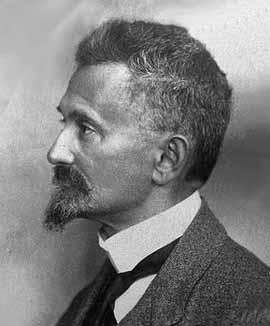
\includegraphics[width=0.4\textwidth]{felix-hausdorff.jpg}
    \caption[Felix Hausdorff,~1868--1942]{Felix Hausdorff\footnote{Převzato z~\cite{OConnorHausdorff2025}},~1868--1942}
    \label{fig:felix-hausdorff}
\end{figure}

\subsection{Definice Hausdorffovy míry}\label{subsec:hd-mira-definice}

\begin{definition}\label{def:hd-mira-delta}
    Nechť je dána množina $F\subseteq\R^n$ a $s>0$. Pak pro každé $\delta>0$ definujeme zobrazení
    \[\hausdorffdeltameasure{s}{\delta}(F)=\inf\set{\sum_{i=1}^{\infty}(\diam{F_i})^s\;\middle|\;F\subseteq\bigcup_{i=1}^\infty F_i\;,\;\diam{F_j}\leqslant\delta\;\text{pro}\;j\in\N}.\]
\end{definition}
Na první pohled si lze všimnout,~že pro $0<\delta_1<\delta_2$ je $\hausdorffdeltameasure{s}{\delta_1}(F)\geqslant\hausdorffdeltameasure{s}{\delta_2}(F)$. Jinými slovy, funkce $\delta\mapsto\hausdorffdeltameasure{s}{\delta}(M)$ je nerostoucí. Toto není nikterak těžké si rozmyslet,~neboť pro $\delta_1<\delta_2$ existuje $\delta_1$-pokrytí $\mathcal{F}_1$,~takové,~že je podpokrytím $\delta_2$-pokrytí $\mathcal{F}_2$ množiny $F$,~tedy $\mathcal{F}_1\subseteq\mathcal{F}_2$. To znamená,~že
\begin{align*}
    \hausdorffdeltameasure{s}{\delta_1}(F)&=\inf\set{\sum_{U\in\mathcal{F}_1}(\diam{U})^s\;\middle|\;\text{$\mathcal{F}_1$ je $\delta_1$-pokrytí $\mathcal{F}$}}\\
    &\geqslant\inf\set{\sum_{U\in\mathcal{F}_2}(\diam{U})^s\;\middle|\;\text{$\mathcal{F}_2$ je $\delta_2$-pokrytí $\mathcal{F}$}}=\hausdorffdeltameasure{s}{\delta_2}(F).
\end{align*}
Zároveň je z~definice \ref{def:hd-mira-delta} zjevné,~že $\mathcal{H}_\delta^s(F)\geqslant 0$.
\begin{definition}[Hausdorffova míra]\label{def:hausdorffova-mira}
    Nechť $F\subseteq\R^n$. Pak pro množinu $F$ definujeme \emph{$s$-dimenzionální Hausdorffovu míru}\index{míra!Hausdorffova} jako
    \[\hausdorffmeasure{s}(F)=\lim_{\delta\to 0}\hausdorffdeltameasure{s}{\delta}(F).\]
\end{definition}
Z přechodzího je zjevné,~že limita v~definici \ref{def:hausdorffova-mira} vždy existuje.

Bude dobré se přesvědčit,~že je Hausdorffova míra mírou ve smyslu definice \ref{def:prostor-s-mirou}. Začneme však otázkou. \emph{Na jaké množině je potřeba Hausdorffovu míru $\hausdorffmeasure{s}$ uvažovat?} Odpověď nám poskytují tzv. \emph{borelovské množiny}\index{množina!borelovská},~které jsou pojmenovány po francouzském matematikovi \name{Émile Borelovi} (1871--1956).
\begin{figure}[h]
    \centering
    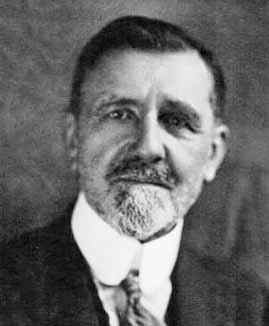
\includegraphics[width=0.4\textwidth]{Emile-Borel.jpeg}
    \caption[Émile Borel,~1871--1956]{Émile Borel\footnote{Převzato z~\cite{OConnorBorel2025}},~1871--1956}
\end{figure}
Borelovské množiny hrají podstatnou roli v~tzv. \emph{Deskriptivní teorii množin}. Nebudeme si zde vykládat všechny souvislosti,~vystačíme si se základem. Takto nazýváme všechny množiny,~které lze získat iteracemi operacemi spočetného sjednocení, průniku a doplňku otevřených množin z~$X$. Označme systém takových množin jako $\mathcal{G}$. Na tomto základě pak definujeme tzv. \emph{$\sigma$-algebru borelovských množin na $X$}:
\[\borelsigmaalgebra(X)=\bigcap_{\substack{\mathcal{F}\supseteq\mathcal{G}\\\text{$\mathcal{F}$ je $\sigma$-algebra}}}\mathcal{F}.\]
Jinými slovy,~$\borelsigmaalgebra(X)$ je nejmenší $\sigma$-algebra generovaná\footnote{Obecně $\sigma$-algebra $\mathcal{A}$ je generovaná množinou $X$,~když
\[\mathcal{A}=\bigcap_{\substack{\mathcal{F}\supseteq X\\\text{$\mathcal{F}$ je $\sigma$-algebra}}}\mathcal{F}.\]
Tento fakt se někdy značí $\mathcal{A}=\sigma(X)$.} všemi otevřenými množinami z~$X$.

Nás speciálně bude zajímat $\sigma$-algebra $\borelsigmaalgebra(\R^n)$. Nejdříve si však dokážeme dvě pomocná lemmata.
\begin{lemma}[$\sigma$-subaditivita Hausdorffovy míry]\label{lem:Hausdorffova-mira-subaditivita}
    Nechť jsou dány množiny $A_1,A_2,\ldots$,~kde $A_i\subseteq X$ pro každé $i\in\N$. Pak pro každé $s\geqslant 0$ platí
    \[\hausdorffmeasure{s}\left(\bigcup_{i=1}^\infty A_i\right)\leqslant\sum_{i=1}^{\infty}\hausdorffmeasure{s}(A_i).\]
\end{lemma}
\begin{proof}
    Nechť $s\geqslant 0$ a dále budiž dáno $\varepsilon>0$. Pro každé $i\in\N$ a $\delta>0$ mějme pokrytí
    \[\mathcal{F}_i=\set{F_{i,1},F_{i,2},\dots}\]
    množiny $A_i$,~takové,~že platí
    \[\sum_{j=1}^{\infty}(\diam{F_{i,j}})^s\leqslant\hausdorffdeltameasure{s}{\delta}(A_i)+\dfrac{\varepsilon}{2^i}.\]
    Systém $\bigcup_{i=1}^\infty\mathcal{F}_i$ tedy tvoří $\delta$-pokrytí množiny $A=\bigcup_{i=1}^\infty A_i$. Celkově
    \begin{align*}
        \hausdorffdeltameasure{s}{\delta}\left(\bigcup_{i=1}^\infty A_i\right)&\leqslant\sum_{i,j\in\N}(\diam{F_{i,j}})^s=\sum_{i=1}^{\infty}\sum_{j=1}^{\infty}(\diam{F_{i,j}})^s\leqslant\sum_{i=1}^{\infty}\left(\hausdorffdeltameasure{s}{\delta}(A_i)+\dfrac{\varepsilon}{2^i}\right)\\
        &=\sum_{i=1}^{\infty}\hausdorffdeltameasure{s}{\delta}(A_i)+\varepsilon.
    \end{align*}
    Limitním přechodem $\delta\to 0$ a aplikací Leviho věty\footnote{\emph{Leviho věta o~záměně pořadí limity a Lebesgueova integrálu} říká,~že je-li posloupnost nezáporných měřitelných funkcí $\set{f_n}_{n=1}^\infty$ neklesající,~tj.
    \[f_1\leqslant f_2\leqslant\dots\]
    na prostoru $(X,\mathcal{A},\mu)$ a zároveň $\lim_{n\to\infty}f_n(x)=f(x)$ pro každé $x\in X$,~pak
    \[\lim_{n\to\infty}\int_X f_n\dx[\mu]=\int_X \lim_{n\to\infty}f_n\dx[\mu].\]
    Zde je speciálně $\mu$ aritmetická míra, $X=\N$,~a $f_n(i)$ lze volit např. $\hausdorffdeltameasure{s}{1/n}(A_i)$. Z~Heineho věty víme,~že
    \[\lim_{n\to\infty}\hausdorffdeltameasure{s}{1/n}(A_i)=\lim_{\delta\to 0}\hausdorffdeltameasure{s}{\delta}(A_i)=\hausdorffmeasure{s}(A_i).\]
    }
    dostáváme
    \begin{align*}
        \hausdorffmeasure{s}\left(\bigcup_{i=1}^\infty A_i\right)&=\lim_{\delta\to 0}\hausdorffdeltameasure{s}{\delta}\left(\bigcup_{i=1}^\infty A_i\right)\leqslant\lim_{\delta\to 0}\sum_{i=1}^{\infty}\hausdorffdeltameasure{s}{\delta}(A_i)+\varepsilon=\sum_{i=1}^{\infty}\lim_{\delta\to 0}\hausdorffdeltameasure{s}{\delta}(A_i)+\varepsilon\\
        &=\sum_{i=1}^{\infty}\hausdorffmeasure{s}(A_i)+\varepsilon.
    \end{align*} 
\end{proof}
\begin{lemma}\label{lem:hausdorffova-mira-sigma-aditivita-kladna-vzdalenost}
    Nechť $(X,\varrho)$ je metrický prostor,~kde $X\subseteq\R^n$,~a $A,B\subseteq X$,~takové,~že pro jejich vzdálenost platí $\varrho(A,B)>0$. Pak pro každé $s\geqslant 0$ platí
    \[\hausdorffmeasure{s}(A\cup B)=\hausdorffmeasure{s}(A)+\hausdorffmeasure{s}(B).\]
\end{lemma}
\begin{proof}
    Nerovnost $\hausdorffmeasure{s}(A\cup B)\leqslant\hausdorffmeasure{s}(A)+\hausdorffmeasure{s}(B)$ je zřejmá ze $\sigma$-subaditivity Hausdorffovy míry (viz lemma \ref{lem:Hausdorffova-mira-subaditivita}).

    Bez újmy na obecnosti předpokládejme,~že $\hausdorffmeasure{s}(A\cup B)<\infty$. Mějme libovolné $\varepsilon>0$. Zvolme $\delta$-pokrytí $\mathcal{F}=\set{F_1,F_2,\ldots}$ množiny $A\cup B$,~takové,~že
    \[\sum_{i=1}^{\infty}(\diam{F_i})^s\leqslant\hausdorffdeltameasure{s}{\delta}(A\cup B)+\varepsilon.\]
    Opět bez újmy na obecnosti lze předpokládat,~že pro každé $i\in\N$ je $\diam{F_i}<\varrho(A,B)$. V~opačném případě bychom $F_i$ pokryli množnami s~menším průměrem. Z~toho pak plyne,~že každá z~množin $F_i$ má neprázdný průnik s~nejvýše jednou z~množin $A,B$,~tzn. z~pokrytí $\mathcal{F}$ lze vybrat dva disjunktní podsystémy $\mathcal{F}_A$ a~$\mathcal{F}_B$,~přičemž $\bigcup\mathcal{F}_A\supseteq A$ a $\bigcup\mathcal{F}_B\supseteq B$. Tedy celkově s~užitím předchozího lemmatu \ref{lem:Hausdorffova-mira-subaditivita} máme
    \begin{align*}
        \hausdorffdeltameasure{s}{\delta}(A)+\hausdorffdeltameasure{s}{\delta}(B)&\leqslant\hausdorffdeltameasure{s}{\delta}\left(\bigcup_{F\in\mathcal{F}_A}F\right)+\hausdorffdeltameasure{s}{\delta}\left(\bigcup_{F\in\mathcal{F}_B}F\right)\\
        &\leqslant\sum_{F\in\mathcal{F}_A}(\diam{F})^s+\sum_{F\in\mathcal{F}_B}(\diam{F})^s\\
        &\leqslant\sum_{i=1}^{\infty}(\diam{F_i})^s\leqslant\hausdorffdeltameasure{s}{\delta}(A\cup B)+\varepsilon.
    \end{align*}
    Pro $\delta\to 0$ dostáváme
    \[\hausdorffmeasure{s}(A)+\hausdorffmeasure{s}(B)\leqslant\hausdorffmeasure{s}(A\cup B)+\varepsilon\]
\end{proof}

\begin{definition}[Vnější míra]\label{def:vnejsi-mira}
    Nechť $(X,\mathcal{A})$ je měřitelný prostor. Zobrazení $\mapping{\mu^*}{\mathcal{A}}{\langle0,\infty\rangle}$ nazveme \emph{vnější mírou}\index{míra!vnější} na $\mathcal{A}$, pokud platí:
    \begin{enumerate}[label=(\alph*)]
        \item\label{def:vnejsi-mira-prazdna-mnozina} $\mu^*(\emptyset)=0$,
        \item\label{def:vnejsi-mira-monotonie} Pokud $A,B\in\mathcal{A}$ a $A\subseteq B$, pak $\mu^*(A)\leqslant\mu^*(B)$.
        \item\label{def:vnejsi-mira-sigma-subaditivita} Je-li $A_1,A_2,\ldots$ posloupnost množin, kde $A_i\in\mathcal{A}$ pro každé $i\in\N$, pak
        \[\mu^*\left(\bigcup_{i=1}^\infty A_i\right)\leqslant\sum_{i=1}^{\infty}\mu^*(A_i).\]
    \end{enumerate}
\end{definition}

Vnější míra představuje zobecnění toho, co jsme měli možnost vidět již v sekci \ref{sec:lebesgueova-mira} týkající Lebesgueovy míry\footnote{Jedná se slabší požadavek, tzn. každá míra je vnější mírou, opačné tvrzení však neplatí.}. Tu jsme definovali na základě tzv. \emph{vnější Lebesgueovy míry} (viz definice \ref{def:vnejsi-lebegueova-mira}), která sice sama o sobě míru nepředstavovala, nicméně při restrikci na "správný" systém množin jsme konstatovali, že se již jedná o míru. Lze se přesvědčit, že vnější Lebesgueova míra $\lebesgueoutermeasure{n}$ je vnější mírou ve smyslu definice \ref{def:vnejsi-mira} výše. Podobné pozorování lze učinit i pro Hausdorffovu míru $\hausdorffmeasure{s}$. Platnost podmínky \ref{def:vnejsi-mira-sigma-subaditivita} jsme dokázali v lemmatu \ref{lem:Hausdorffova-mira-subaditivita} a o platnosti \ref{def:vnejsi-mira-prazdna-mnozina} a \ref{def:vnejsi-mira-monotonie} se může čtenář velice snadno předvědčit. Tedy Hausdorffova míra na měřitelném prostoru $(X,\mathcal{A})$ je vnější mírou. Navíc pokud vnější míra $\mu^*$ splňuje závěr lemmatu \ref{lem:hausdorffova-mira-sigma-aditivita-kladna-vzdalenost}, pak ji nazýváme \emph{metrickou vnější mírou}\index{míra!metrická}\index{míra!metrická vnější}.

Carathéodoryho kritérium, které jsme si uváděli při zavádění \emph{lebesgueovské měřitelnosti}\index{měřitelnost!lebesgueovská} (viz definice \ref{def:lebesgueovska-meritelnost}). Ta jednoduše říkala, že rozdělením libovolné množiny $G$ pomocí pěvně zvolené množiny $A$ lze stanovit její míru jako součet měr dílčích částí, tzn. $G\cap A$ a $G\setminus A$. Tento koncept lze však rozšířit. Obecně jakákoliv množina je $\mu$-měřitelná, pokud splňuje Carathéodoryho kritérium.
\begin{definition}\label{def:meritelnost}
    Nechť $\mu$ je míra a $A\subseteq X$. Množina $A$ je $\mu$-měřitelná, pokud pro každé $G\subseteq X$ platí
    \[\mu(G)=\mu(G\cap A)+\mu(G\setminus A).\]
\end{definition}
Speciálně nyní ukážeme platnost následujícího tvrzení \ref{thm:hs-meritelnost-borel-mnozin}.
\begin{theorem}\label{thm:hs-meritelnost-borel-mnozin}
    Nechť $(X,\varrho)$ je metrický prostor. Pak každá množina $A\in\borelsigmaalgebra(X)$ je $\hausdorffmeasure{s}$-měřitelná pro každé $s\geqslant 0$.
\end{theorem}
\begin{proof}
    Není těžké si rozmyslet, že $\borelsigmaalgebra(X)$ vyjma otevřených množin obsahuje též všechny uzavřené\footnote{Plyne z uzavřenosti na doplněk.}. Volme tedy uzavřenou množinu $A\in\borelsigmaalgebra(X)$, $G\subseteq X$ a $s\geqslant 0$. Ze $\sigma$-subaditivity plyne nerovnost
    \[\hausdorffmeasure{s}(G)\leqslant\hausdorffmeasure{s}(G\cap A)+\hausdorffmeasure{s}(G\setminus A).\]
    Pro důkaz opačné nerovnosti definujeme posloupnost množin $P_0,P_1,P_2,\ldots$ následovně:
    \begin{align*}
        P_0&=\set{x\in G\mid\varrho(x,A)\geqslant 1},\\
        P_i&=\set{x\in G\;\middle|\;\dfrac{1}{i+1}\leqslant\varrho(x,A)\leqslant\dfrac{1}{i}}\;,\;i\geqslant 1.
    \end{align*}
    Pro libovolnou dvojici množin z podposloupnosti $P_0,P_2,P_4,\ldots$ platí, že jejich vzdálenosti jsou kladné. Z faktu, že $\hausdorffmeasure{s}$ je metrická (viz lemma \ref{lem:hausdorffova-mira-sigma-aditivita-kladna-vzdalenost}) a monotonie plyne
    \[\sum_{i=1}^{m}\hausdorffmeasure{s}(P_{2i})=\hausdorffmeasure{s}\left(\bigcup_{i=0}^m P_{2i}\right)\leqslant\hausdorffmeasure{s}(G)\]
    pro všechna $m\in\N$. Podobně pro liché členy $\sum_{i=0}^{m}\hausdorffmeasure{s}(P_{2i+1})\leqslant\hausdorffmeasure{s}(G)$. Tzn. řada $\sum_{i=0}^{\infty}\hausdorffmeasure{s}(P_i)$ je konvergentní. Zároveň platí
    \[\varrho\left(\bigcup_{i=0}^m P_i,G\cap A\right)>0,\]
    pro každé $m\in\N$, tedy lze psát
    \begin{align*}
        \hausdorffmeasure{s}(G\setminus A)&\leqslant\hausdorffmeasure{s}\left(\bigcup_{i=0}^m P_i\right)+\hausdorffmeasure{s}\left(\bigcup_{i=m+1}^\infty P_i\right)\\
        &\leqslant\hausdorffmeasure{s}(G)-\hausdorffmeasure{s}(G\cap A)+\sum_{i=m+1}^{\infty}\hausdorffmeasure{s}(P_i).
    \end{align*}
    Pro $m\to\infty$ dostáváme
    \[\hausdorffmeasure{s}(G\setminus A)\leqslant\hausdorffmeasure{s}(G)-\hausdorffmeasure{s}(G\cap A)\]
    z čehož již plyne požadovaná nerovnost.
\end{proof}
\begin{corollary}\label{cor:hausdorffova-mira-je-mira}
    Trojice $(X,\borelsigmaalgebra(X),\hausdorffmeasure{s})$,~kde $X$ je libovolná množina a $s\geqslant 0$,~tvoří prostor s~mírou.
\end{corollary}

Nyní již můžeme zobrazení $\hausdorffmeasure{s}$ nazývat mírou oprávněně. Pojďme se podívat na nějaké příklady.
\begin{example}
    Pro $s=0$ představuje zobrazení $\hausdorffmeasure{s}$ obyčejnou aritmetickou míru\index{míra!aritmetická},~tzn. pro konečnou množinu $A\subseteq\R^n$ je $\hausdorffmeasure{0}(A)=|A|$. Toto není těžké ukázat. Mějme množinu $A=\set{x_1,x_2,\ldots,x_n}$. Zvolíme-li
    \[\delta<\dfrac{1}{2}\cdot\min\set{\varrho_e(x_i,x_j)\mid 1\leqslant i,j\leqslant n},\]
    pak pro $\delta$-pokrytí $\mathcal{F}=\set{F_1,F_2,\ldots,F_n}$ takové,~že $x_i\in F_i$ pro každé $i$ máme
    \[\sum_{i=1}^{n}(\diam{F_i})^0=\sum_{i=1}^{n}1=n.\]
    Není těžké si rozmyslet,~že $n$ je nejmenší počet množin o~průměru nejvýše $\delta$,~takových,~aby pokrývaly množinu $A$. Zároveň pro libovolné $\varepsilon>0$ je potřeba nejvýše $n$-koulí o~poloměru $\varepsilon/2$ se středy v~$x_i$ pro pokrytí $A$. Tzn.~$\hausdorffmeasure{0}(A)=|A|=n$.
\end{example}

V rámci tohoto textu jsme se již zabývali jiným typem míry a to tzv. \emph{lebesgueovou mírou} (viz sekce \ref{sec:lebesgueova-mira}). Ta pro nás hrála důležitou roli v jednom možném pojetí \emph{box-counting dimenze} (viz sekce \ref{sec:box-counting-dimenze}). Lze ukázat, že pro množinu $F\subseteq\R^n$ je
\[\hausdorffmeasure{n}(F)=\dfrac{1}{v_n}\lebesguemeasure{n}(F),\]
kde $v_n$ je objem (míra) jednotkové koule v $\R^n$. Čtenář snad promine, že tento fakt zde ponecháme bez důkazu. \citep[str. 45]{Falconer2014}

\subsection{Stručně k vlastnostem Hausdorffovy míry}\label{subsec:vlastnosti-hausdorffovy-miry}

Na chvíli se ještě zastavíme u vlastností Hausdorffovy míry. Již jsme společně dokázali, že Hausdorffova míra je skutečně mírou, tzn. splňuje všechny základní vlastnosti, které jsme si představili ve větě \ref{thm:mira-vlastnosti} (viz sekce \ref{sec:prostory-s-mirou}). V tomto ohledu tedy netřeba již nic dalšího dokazovat. Nicméně podobně jako v případě \emph{box-counting dimenze} (viz podsekce \ref{subsec:vlastnosti-bc-dimenze}) se i zde podíváme, jak se Hausdorffova míra chová vůči \emph{lipschitzovským zobrazením}\index{zobrazení!lipschitzovské}.
\begin{theorem}\label{thm:hd-dimenze-lipschitzovske-zobrazeni}
    Nechť $F\subseteq\R^n$ v metrickém prostoru $(\R^n,\varrho)$ a zobrazení $\mapping{f}{F}{\R^n}$ je lipschitzovské\footnote{Tvrzení lze zformulovat obecněji pro tzv. \emph{hölderovská zobrazení}\index{zobrazení!hölderovské}, tedy zobrazení $f$ splnující
    \[\varrho(f(x),f(y))\leqslant K(\varrho(x,y))^\alpha.\]
    kde $\alpha>0$. Pak pro $F\subseteq\R^n$ platí
    \[\hausdorffmeasure{s/\alpha}(f(F))\leqslant K^{s/\alpha}\hausdorffmeasure{s}(F).\]
    My si však vystačíme se speciálním případem.} s konstantou $K>0$. Pak pro každé $s\geqslant 0$ platí
    \[\hausdorffmeasure{s}(f(F))\leqslant K^s\hausdorffmeasure{s}(F).\]
\end{theorem}
\begin{proof}
    Nechť $\mathcal{F}=\set{F_1,F_2,\ldots}$ je $\delta$-pokrytí $F$. Pak
    \[\diam(f(F\cap F_i))\leqslant K\diam(F\cap F_i)\leqslant K\diam{F_i},\]
    což znamená, že $\mathcal{G}=\set{F\cap F_1,F\cap F_2,\ldots}$ je $K\delta$-pokrytí $f(F)$. Z toho plyne, že
    \[\sum_{i=1}^{\infty}(\diam(f(F\cap F_i)))^s\leqslant K^s\sum_{i=1}^{\infty}(\diam{F_i})^s\]
    a tedy $\hausdorffdeltameasure{s}{K\delta}(f(F))\leqslant K^s\hausdorffdeltameasure{s}{\delta}(F)$. Pro $\delta\to 0$ máme požadovaný výsledek.
\end{proof}
(Převzato z \citep[str. 46]{Falconer2014}.)

Z toho speciálně plyne důsledek týkající se podobností.
\begin{corollary}\label{cor:hd-dimenze-podobnost}
    Nechť $F\subseteq\R^n$ v metrickém prostoru $(\R^n,\varrho)$ a zobrazení $\mapping{f}{F}{\R^n}$ je podobnost\index{podobnost}, tzn. existuje $K>0$ takové, že pro každé $x,y\in F$ platí
    \[\varrho(f(x),f(y))=K\varrho(x,y).\]
    Pak pro každé $s\geqslant 0$ platí
    \[\hausdorffmeasure{s}(f(F))=K^s\hausdorffmeasure{s}(F).\]
\end{corollary}
\begin{proof}
    K podobnosti $f$ existuje inverzní zobrazení $f^{-1}$ s koeficientem $L=1/K$. Z věty \ref{thm:hd-dimenze-lipschitzovske-zobrazeni} tedy plyne, že
    \[\hausdorffmeasure{s}(F)=\hausdorffmeasure{s}(f^{-1}(f(F)))\leqslant\dfrac{1}{K^s}\hausdorffmeasure{s}(f(F))\]
    nebo-li $\hausdorffmeasure{s}(f(F))\geqslant K^s\hausdorffmeasure{s}(F)$. Opačnou nerovnost získáme aplikací věty \ref{thm:hd-dimenze-lipschitzovske-zobrazeni} na zobrazení $f$.
\end{proof}

\subsection{Hausdorffova dimenze}\label{subsec:hausdorffova-dimenze}

Středobodem této sekce je tzv. \emph{Hausdorffova dimenze}\index{dimenze!Hausdorffova}. Na úvod si dokážeme jedno jednoduché tvrzení týkající se Hausdorffovy míry.
\begin{theorem}\label{thm:hodnoty-hausdorffovy-miry}
    Nechť $0\leqslant s<t<\infty$ a $F\subseteq X$. Pak platí:
    \begin{enumerate}[label=(\roman*)]
        \item\label{thm:hd-dimenze-konecna} $\hausdorffmeasure{s}(F)<\infty\implies\hausdorffmeasure{t}(F)=0$,
        \item\label{thm:hd-dimenze-nekonecno} $\hausdorffmeasure{t}(F)>0\implies\hausdorffmeasure{s}(F)=\infty$.
    \end{enumerate}
\end{theorem}
\begin{proof}
    Mějme $\delta$-pokrytí $\mathcal{F}=\set{F_1,F_2,\ldots}$,~takové,~že
    \[\sum_{i=1}^{\infty}(\diam{F_i})^s\leqslant\hausdorffdeltameasure{s}{\delta}(F)+\varepsilon\;,\;\varepsilon>0.\]
    Pak
    \[\hausdorffdeltameasure{t}{\delta}(F)\leqslant\sum_{i=1}^{\infty}(\diam{F_i})^t\leqslant\delta^{t-s}\sum_{i=1}^{\infty}(\diam{F_i})^s\leqslant\delta^{t-s}(\hausdorffdeltameasure{s}{\delta}(F)+\varepsilon).\]
    Tzn.~$\hausdorffdeltameasure{t}{\delta}(F)\leqslant\delta^{t-s}\hausdorffdeltameasure{s}{\delta}(F)$. Pro $\delta\to 0$ dostaneme body \ref{thm:hd-dimenze-konecna} a \ref{thm:hd-dimenze-nekonecno}.
\end{proof}
(Převzato z~\citep[str. 68]{Mattila1995}.)

Z věty \ref{thm:hodnoty-hausdorffovy-miry} lze vidět,~že Hausdorffova míra dává smysl jen pro určitou hodnotu $s$. Pro "příliš velké" $s$ bude hodnota vždy $0$,~naopak pro "moc malé" $s$ bude jeho hodnota rovna $\infty$ (viz obrázek \ref{fig:hausdorffova-dimenze-graf}).
\begin{figure}[h]
    \centering
    \includegraphics{ch02-hausdorffova-dimenze-graf.pdf}
    \caption{Graf funkce $f(s)=\hausdorffmeasure{s}(F)$,~kde $F\subseteq\R^n$.}
    \label{fig:hausdorffova-dimenze-graf}
\end{figure}
Této kritické hodnotě $s$ říkáme \emph{Hausdorffova dimenze}\index{dimenze!Hausdorffova}.
\begin{definition}[Hausdorffova dimenze]\label{def:hausdorffova-dimenze}
    Nechť $F\subseteq\R^n$. Hausdorffovou dimenzí\footnote{Též někdy nazývaná \emph{Hausdorffova-Bezikovičova dimenze}\index{dimenze!Hausdorffova-Bezikovičkova}. }\index{dimenze!Hausdorffova} množiny $F$ nazveme hodnotu
    \[\dimH{F}=\inf\set{s\geqslant 0\mid\hausdorffmeasure{s}(F)=0}=\sup\set{s\geqslant 0\mid\hausdorffmeasure{s}(F)=\infty}.\]
\end{definition}
Hodnota $\hausdorffmeasure{s}(F)$ pro $s=\dimH{F}$ může být různá,~tzn. může platit,~že $\hausdorffmeasure{s}(F)=\infty$,~$\hausdorffmeasure{s}(F)=0$ a nebo se může jednat o~konečné nenulové číslo,~tj. $0<\hausdorffmeasure{s}(F)<\infty$.

Nyní se podívejme na příklad výpočtu. Podobně, jako v případě box-counting dimenze, i zde budeme nezávisle určovat horní a dolní odhad.
\begin{example}[Sierpińského trojúhelník]\label{ex:sierpinskeho-trojuhelnik-hd-dimenze}
    V tomto případě se podíváme na dvě možnosti, jak dojít k výsledku. Celý Sierpińského trojúhelník si označme $S$.
    \begin{itemize}
        \item V $k$-té iteraci, kde $k=0,1,2,\ldots$, vzniknou 3 nové trojúhelníky o obsahu $1/4$ obsahu původního trojúhelníka, tzn. jejich celkový počet je $t=3^k$. Uvažíme-li $\delta$-pokrytí
        \[\mathcal{K}=\set{K_\delta^1(x_1),K_\delta^2(x_2),\ldots,K_\delta^t(x_t),\emptyset,\emptyset,\ldots}\]
        kde $x_1,x_2,\ldots,x_t\in S_k$ a $\delta\leqslant 2^{-k}/2=2^{-k-1}$, pak
        \[\hausdorffdeltameasure{s}{2^{-k}}(S_k)\leqslant\sum_{i=1}^{3^k}(2^{-k})^s=3^k2^{-ks}=1.\]
        Pro $k\to\infty$ je $\hausdorffmeasure{s}(S)\leqslant 1$. Poslední rovnost nastává právě pro $s=\ln{3}/\ln{2}$.

        Nyní ukážeme, že $\hausdorffmeasure{s}(S)\geqslant 3^{-s}=1/2$. Zvolme $\delta$-pokrytí $\mathcal{F}=\set{F_1,F_2,\ldots}$, takové, že
        \begin{equation}\label{eq:volba-delta-pokryti-F}
            2^{-k-1}\leqslant\diam{F_i}<2^{-k},
        \end{equation}
        kde $i\in\N$. Lze si rozmyslet, že každá z množin $F_i$ má neprázdný průnik s nejvýše dvěma dílčími trojúhelníky. Zvolíme-li $j\geqslant k$, pak každá z množin $F_i$ má průnik maximálně s $3^{j-k}$ trojúhelníky v $j$-té iteraci, resp.
        \[3^{j-k}=3^j2^{-ks}\leqslant2^j3^s(\diam{F_i})^s,\]
        jak plyne z volby pokrytí $\mathcal{F}$ v \eqref{eq:volba-delta-pokryti-F}. Pokud navíc pro každé $i\in\N$ platí, že
        \[3^{-j-1}\leqslant\diam{F_i},\]
        pak každá z množin $F_i$ má neprázdný průnik s nejvýše $3^j$ trojúhelníky. Tedy pro jejich počet platí
        \[3^j\leqslant\sum_{i=1}^{\infty}3^j3^s(\diam{F_i})^s,\]
        přičemž úpravou už získáme požadovanou nerovnost.
        \item Druhá varianta výpočtu je sice méně rigorózní, avšak podstatně jednodušší. Sierpińského trojúhelník sestává ze tří kopií sebe samotného, přičemž každá z nich je obrazem původního obrazce $S$ v podobnosti s koeficientem $K=1/2$. Označme si dané části $S_1,S_2$ a $S_3$, tj. $S=S_1\cup S_2\cup S_3$. Tedy podle $\sigma$-aditivity Hausdorffovy míry a důsledku \ref{cor:hd-dimenze-podobnost} můžeme psát
        \begin{align*}
            \hausdorffmeasure{s}(S)&=\hausdorffmeasure{s}(S_1)+\hausdorffmeasure{s}(S_2)+\hausdorffmeasure{s}(S_3)\\
            &=\left(\dfrac{1}{2}\right)^s\hausdorffmeasure{s}(S)+\left(\dfrac{1}{2}\right)^s\hausdorffmeasure{s}(S)+\left(\dfrac{1}{2}\right)^s\hausdorffmeasure{s}(S)\\
            &=3\left(\dfrac{1}{2}\right)^s\hausdorffmeasure{s}(S).
        \end{align*}
        Budeme-li předpokládat, že $\hausdorffmeasure{s}(S)<\infty$ (jak jsme již viděli z předchozího výpočtu, jedná se o netriviální předpoklad) pro $s=\dimH{S}$, pak z rovnosti $1=3(1/2)^s$ lze dopočítat, že $s=\ln{3}/\ln{2}$.
    \end{itemize}
\end{example}
(Převzato a upraveno z \citep[str. 53]{Falconer2014}.)

Myšlenku druhého výpočtu z příkladu \ref{ex:sierpinskeho-trojuhelnik-hd-dimenze} ještě rozvedeme v kapitole \ref{chapter:klasifikace-fraktalu}, konkrétně v sekci \ref{sec:ifs} věnované systémům iterovaných funkcí\index{systém iterovaných funkcí}.

Jako poslední zkusme postavit Hausdorffovu dimenzi proti box-counting dimenzi, kterou jsme si představili v sekci \ref{sec:box-counting-dimenze}. 
\chapter{Hausdorffův metrický prostor}\label{chapter:hausdorffuv-mp}

V této kratší kapitole se podíváme na některé výsledky související s~tzv. \emph{Hausdorffovým metrickým prostorem},~s nímž se ještě dále setkáme. Pro připomenutí záležitostí ohledně metrických prostorů celkově doporučuji čtenáři se podívat do sekce~\ref{sec:zakladni-pojmy-a-znaceni} v~kapitole~\ref{chapter:teorie-miry-a-dimenze}. Pokud by čtenáře zajímaly další podrobnosti,~doporučuji se podívat do knihy \citep[str. 71]{Edgar2008}.

\section{Hausdorffova metrika}\label{sec:hausdorffova-metrika}

Jako první se podíváme na tzv. \emph{Hausdorffovu metriku}\index{Hausdorffův metrický prostor!Hausdorffova metrika}.
\begin{definition}[Hausdorffova metrika]\label{def:hausdorffova-metrika}
    Hausdorffovou metrikou\index{Hausdorffův metrický prostor!Hausdorffova metrika} (vzdálenost) nazýváme takové zobrazení $\mapping{\hausdorffmetric}{\powset{X}^2}{\langle0,\infty\rangle}$,~kde pro každé $A,B\in\powset{X}$ platí
    \[\hausdorffmetric(A,B)=\inf\set{\delta>0\;\middle|\;A\subseteq (B)_\delta\;,\;B\subseteq (A)_\delta}.\]
\end{definition}
Podobně jako v~případě Lebesgueovy míry (viz sekce \ref{sec:lebesgueova-mira},~definice \ref{def:lebesgueovska-meritelnost}) se i~zde nabízí stejná otázka: \emph{Co nás opravňuje nazývat Hausdorffovu metriku metrikou?} Odpovědí je,~že zatím nic,~neboť tato definice sama o~sobě neimplikuje,~že $\hausdorffmetric$ je metrika. V~definici povolujeme totiž případ,~kdy $\hausdorffmetric(A,B)=\infty$ a pro příklady takových množin netřeba chodit daleko. Např. v~$\R$,~když budeme počítat Hausdorffovu metriku množin $\set{0}$ a $\langle 0,\infty)$,~zjistíme,~že $\hausdorffmetric(\set{0},\langle 0,\infty))=\infty$. Podobně budeme-li počítat $\hausdorffmetric(\emptyset,\set{0})$,~dojdeme ke stejnému výsledku. Ovšem i~v případě některých neprázdných omezených množin si lze všimnout nesrovnalostí. Např. pro množiny $(0,1)$ a $(0,1\rangle$ je Hausdorffova metrika nulová,~přestože dané množiny nejsou stejné.

Pokud se však omezíme jen na některé množiny,~bude $\hausdorffmetric$ skutečně metrikou ve smyslu definice \ref{def:metricky-prostor}. Proto se dále zaměříme pouze na takové podmnožiny $X$,~které jsou \emph{neprázdné} a \emph{kompaktní}.
\begin{definition}[Hyperprostor]\label{def:hyperprostor}
    Systém všech neprázdných kompaktních podmnožin množiny $X$ nazýváme \emph{hyperprostor}\index{hyperprostor} a značíme jej $\hyperspace(X)$.
\end{definition}
\begin{proposition}\label{prop:sjednoceni-kompaktnich-mnozin}
    Nechť $A,B\in\hyperspace(X)$. Pak $A\cup B\in\hyperspace(X)$.
\end{proposition}
\begin{proof}
    Neprázdnost $A\cup B$ je zjevná. Sjednocení kompaktních množin je opět kompaktní. Máme-li totiž pokrytí $\mathcal{U}\supseteq A$ a $\mathcal{V}\supseteq B$,~pak z~kompaktnosti $A,B$ víme,~že z~každého z~nich z~nich lze vybrat konečné podpokrytí
    \[\mathcal{U}^\prime=\set{U_{i_1},U_{i_2},\ldots,U_{i_k}}\subset\mathcal{U},\;\text{resp.}\;\mathcal{V}^\prime=\set{V_{j_1},V_{j_2},\ldots,V_{j_\ell}}\subset\mathcal{V},\]
    kde $k,\ell\in\N$. Tedy $\mathcal{U}\cup\mathcal{V}$ tvoří pokrytí $A\cup B$,~resp.
    \[\mathcal{U}\cup\mathcal{V}\supseteq\mathcal{U}^\prime\cup\mathcal{V}^\prime\supseteq A\cup B.\]
\end{proof}
Tvrzení \ref{prop:sjednoceni-kompaktnich-mnozin} lze opět rozšířit indukcí
\begin{corollary}\label{cor:sjednoceni-n-kompaktnich-mnozin}
    Pro $A_1,A_2,\ldots,A_n\in\hyperspace(X)$ platí $\bigcup_{i=1}^n A_i\in\hyperspace(X)$.
\end{corollary}
Pro operaci průniku nebo rozdílu toto tvrzení již neplatí. Např. intervaly $\langle0,1\rangle$ a $\langle2,3\rangle$ jsou uzavřené a omezené,~tedy (podle věty \todo{doplnit odkaz}) jsou kompaktní. Avšak jejich průnik je prázdný. Podobně pro rozdíl stačí uvážit $A\subseteq B$,~tzn. $A\setminus B=\emptyset$.
\begin{theorem}\label{thm:hausdorffova-metrika-je-metrika}
    Nechť $(X,\varrho)$ je metrický prostor,~kde $X\subseteq\R^n$. Pak Hausdorffova metrika $\hausdorffmetric$ je metrikou na $\hyperspace(X)$.
\end{theorem}
\begin{proof}
    Zjevně pro každé $A,B\in\hyperspace(X)$ z~definice platí $\hausdorffmetric(A,B)\geqslant 0$ a $\hausdorffmetric(A,B)=\hausdorffmetric(B,A)$. Z~kompaktnosti množin $A,B$ plyne (podle věty \todo{doplnit odkaz}),~že $A,B$ jsou omezené množiny,~tedy $\hausdorffmetric(A,B)<\infty$.
    
    Pro $A=B$ platí,~že pro každé $\delta>0$ je splňeno $A\subseteq (B)_\delta$ a zároveň $B\subseteq (A)_\delta$,~tzn. $\hausdorffmetric(A,B)=0$. Opačná implikace také platí. Předpokládejme,~že množiny $A,B$ splňují $\hausdorffmetric(A,B)=0$. Pokud $x\in A$,~pak pro každé $\delta>0$ platí,~že $x\in (B)_\delta$,~tzn. $\varrho(x,B)=0$,~a z~uzavřenosti $B$ plyne $x\in B$. Tedy $A\subseteq B$ a analogicky platí i~$B\subseteq A$,~tzn. $A=B$.

    Jako poslední je třeba ukázat platnost trojúhelníkové nerovnosti. Mějme množiny $A,B,C\in\hyperspace(X)$ a $\varepsilon>0$. Pro libovolné $x\in A$ existuje $y\in B$,~takové,~že
    \[\varrho(x,y)<\hausdorffmetric(A,B)+\varepsilon.\]
    Podobně pro $y$ existuje $z\in C$,~takové,~že
    \[\varrho(y,z)<\hausdorffmetric(B,C)+\varepsilon.\]
    Z~toho plyne
    \[\varrho(x,z)\leqslant\varrho(x,y)+\varrho(y,z)<\hausdorffmetric(A,B)+\hausdorffmetric(B,C)+2\varepsilon,\]
    kde pravou stranu nerovnosti označme $\delta$. To znamená,~že $A\subseteq (C)_\delta$ a zároveň $C\subseteq (A)_\delta$. Tudíž
    \[\hausdorffmetric(A,C)\leqslant\hausdorffmetric(A,B)+\hausdorffmetric(B,C)+2\varepsilon.\]
\end{proof}
(Převzato z~\citep[str. 72]{Edgar2008}.)
\begin{definition}[Hausdorffův metrický prostor]\label{def:hausdorffuv-mp}
    Metrický prostor $(\hyperspace(X),\hausdorffmetric)$~nazýváme \emph{Hausdorffův metrický prostor}\index{Hausdorffův metrický prostor} na metrickém prostoru $(X,\varrho)$.
\end{definition}
Nyní si opět připomeňte něco z~terminologie metrických prostorů. Posloupnost $\set{x_n}_{n=1}^\infty$ v~metrickém prostoru $(X,\varrho)$,~se nazývá \emph{cauchyovská}\index{cauchyovská posloupnost},~pokud
\[\forall\varepsilon>0\;\exists n_0\in\N\;\forall n,m>n_0: \varrho(x_n,x_m)<\varepsilon.\]
Obecně neplatí,~že každá cauchyovská posloupnost je konvergentní,~avšak pokud v~$X$ všechny takové posloupnosti jsou konvergentní,~pak $(X,\varrho)$ nazýváme \emph{úplný metrický prostor}\index{metrický prostor!úplný}. O~Hausdorffově metrickém prostoru lze v~tomto ohledu dokázat následující tvrzení.
\begin{theorem}[Úplnost HMP]\label{thm:uplnost-hmp}
    Je-li $(X,\varrho)$ úplný metrický prostor,~pak $(\hyperspace(X),\hausdorffmetric)$ je také úplný metrický prostor.
\end{theorem}
Důkaz věty je už trochu delší,~nicméně lze jej nalézt opět např. v~knize \citep[str. 72]{Edgar2008}.
\section{Kompaktní množiny a~konvergence}\label{sec:konvergence-hmp}

\begin{theorem}\label{thm:konvergence-hmp}
    Nechť $A_1,A_2,\ldots$ je nerostoucí posloupnost množin, kde $A_i\in\hyperspace(X)$ pro každé $i\in\N$. Pak posloupnost $A_1,A_2,\ldots$ konverguje k~množině
    \[A=\bigcap_{i=1}^\infty A_i\]
    v~Hausdorffově metrice.
\end{theorem}
\begin{proof}
    Nechť je dáno $\varepsilon>0$. Zjevně pro každé $i$ je $A\subseteq A_i$, tzn. $A\subseteq(A_i)_\varepsilon$.
    
    Nyní najdeme $i_0$ tak, že $\hausdorffmetric(A,A_i)<\varepsilon$ pro každé $i\geqslant i_0$. Systém
    \[\mathcal{F}=\set{(A_i)_\varepsilon}\cup\set{X\setminus A_i\mid i\in\N}\]
    tvoří otevřené pokrytí množiny $A_1$. Podle předpokladu je však $A_1$ kompaktní, tedy z~$\mathcal{F}$ lze vybrat konečné podpokrytí. Specificky existuje $i_0\in\N$ takové, že systém
    \[\mathcal{G}=\set{X\setminus A_{i_0}}\cup\set{(A)_\varepsilon}\]
    pokrytím $A_1$ a~$\mathcal{G}\subseteq\mathcal{F}$ (viz obrázek~\ref{fig:konvergence-hmp}). Z~toho plyne, že $A_{i_0}\subseteq (A)_\varepsilon$, a~tedy pro všechna $i\geqslant i_0$ je $\hausdorffmetric(A,A_i)<\varepsilon$.
\end{proof}
\begin{figure}[h]
    \centering
    \includegraphics{ch03-ilustrace-vety-o-konvergenci.pdf}
    \caption{Ilustrace věty~\ref{thm:konvergence-hmp}}
    \label{fig:konvergence-hmp}
\end{figure}

V souvislosti s~konvergencí v~prostoru $(\hyperspace(X),\hausdorffmetric)$ nebude na škodu si připomenout jedno známé související tvrzení z~matematické analýzy.
\begin{theorem}\label{thm:cantor}
    Následující tvrzení jsou ekvivalentní:
    \begin{enumerate}[label=(\roman*)]
        \item\label{thm:cantor-uplnost} $(X,\varrho)$ je úplný metrický prostor.
        \item\label{thm:cantor-nekl-posl-mnozin} Je-li $A_1,A_2,\ldots$ neklesající posloupnost uzavřených množin v~$X$ takových, že $\diam{A_i}\to 0$ pro každé $i\in\N$, pak existuje $x\in X$ splňující
        \[\bigcap_{i=1}^\infty A_i=\set{x}.\]
    \end{enumerate}
\end{theorem}
Věta~\ref{thm:cantor} je v~podstatě rozšířením Cantorova principu\index{Cantorův princip}\index{princip!Cantorův} vnořených intervalů v~$\R$. Speciálně z~toho vyplývá, že i~v Hausdorffově metrickém prostoru platí podmínka~\ref{thm:cantor-nekl-posl-mnozin}, neboť z~věty~\ref{thm:uplnost-hmp} víme, že $(\hyperspace(X),\hausdorffmetric)$ tvoří úplný metrický prostor.

\begin{theorem}\label{thm:stejnometrna-konvergence-hmp}
    Nechť $(X,\varrho_1),(Y,\varrho_2)$ jsou metrické prostory a~zobrazení $\set{f_i}_{i=1}^\infty$, kde $\mapping{f_i}{X}{Y}$ pro každé $i\in\N$ a~$f_j\rightrightarrows f$ pro $j\to\infty$ na $X$ (viz podsekce \ref{subsec:bodova-stejnomerna-konvergence}).\index{konvergence!stejnoměrná} k~$f$. Pak posloupnost $f_1(X),f_2(X),\ldots$ konverguje k~$f(X)$ na metrickém prostoru $(\hyperspace(Y),\hausdorffmetric)$.
\end{theorem}
\begin{proof}
    Mějme $\varepsilon>0$. Najdeme $i_0\in\N$ tak, že $\hausdorffmetric(f(X),f_i(X))<\varepsilon$ pro $i\geqslant i_0$. Funkce $f_1,f_2,\ldots$ konvergují k~$f$ stejnoměrně, tzn.
    \[\exists i_0\in\N\;\forall i\geqslant i_0\;\forall x\in X:\varrho_2(f(x),f_i(x))<\varepsilon.\]
    Tzn.~pro každé $x\in X$ a~$i\geqslant i_0$ platí
    \[\varrho_2(f(x),f_i(X))\leqslant\varrho_2(f(x),f_i(x))<\varepsilon\]
    a~též
    \[\varrho_2(f_i(x),f(X))\leqslant\varrho_2(f_i(x),f(x))=\varrho_2(f(x),f_i(x))<\varepsilon.\]
    Z~toho vyplývá, že
    \[f(X)\subseteq (f_i(X))_\varepsilon\;\text{a zároveň}\;f_i(X)\subseteq (f(X))_\varepsilon,\]
    neboli $\hausdorffmetric(f(X),f_i(X))<\varepsilon$.
\end{proof}
(Převzato z~\citep[str. 74]{Edgar2008})
\begin{remark}
    Předpoklad stejnoměrné konvergence\index{stejnoměrná konvergence}\index{konvergence!stejnoměrná} ve větě~\ref{thm:stejnometrna-konvergence-hmp} je důležitý. Mějme např. metrický prostor $X=\langle0,1\rangle$ se standardní eukleidovskou metrikou a~definujme posloupnost funkcí
    \[\mapping{f_n}{\langle0,1\rangle}{\R},\;f_n(x)=x^n.\]
    Limitou je funkce $f$, kde
    \[f(x) = \begin{cases}
        0 & x \in \langle0,1),\\
        1 & x = 1.
        \end{cases}\]
    Posloupnost konverguje k~funkci $f$ pouze bodově, nikoliv stejnoměrně. Pro celý interval je $f(X)=\set{0,1}$, nicméně
    \[\hausdorffmetric(\langle0,1\rangle,\set{0,1})=\dfrac{1}{2}.\]
    Tedy neplatí, že $f_n(X)\rightrightarrows f(X)$ v~$(\hyperspace(\R),\hausdorffmetric)$.
\end{remark}
\chapter{Klasifikace fraktálů}\label{chapter:klasifikace-fraktalu}

S kapitolami \ref{chapter:teorie-miry-a-dimenze} a \ref{chapter:hausdorffuv-mp} jsme si v jistém rozsahu ukázali formální podstatu fraktální geometrie. Nicméně pravdou zůstává, že z fraktální útvarů jako takových jsme si toho zatím neukázali (některým z nich jsme se věnovali v kapitole \ref{chapter:uvod_do_fraktalu} v sekci \ref{sec:sobepodobnost} o soběpodobnosti). Proto se nyní podíváme na některé další příklady a především jejich podrobnější klasifikaci dle způsobu jejich vzniku. Na tuto kapitolu též volně navazuje kapitola \ref{chapter:generovani-fraktalu}, kde si fraktály trochu rozebereme z programovacího hlediska.

V této kapitole se zaměříme na tři hlavní metody klasifikace a konstrukce fraktálů - konkrétně na \emph{L-systémy}\index{L-systém}, \emph{systémy iterovaných funkcí (IFS)}\index{Systém iterovaných funkcí} a tzv. \emph{Time Escape algoritmy}\index{Time Escape algoritmus}. Tyto přístupy představují základní postupy, pomocí kterých lze fraktální útvary nejen systematicky vytvářet, ale také analyzovat jejich strukturu a chování z pohledu matematické dynamiky.

\section{L-systémy}\label{sec:L-systemy}

Uvedeme tuto kapitolu s~ohledem na předchozí obsah trochu netradičně a od matematiky se (alespoň zdánlivě) na chvíli odkloníme. Podíváme se na fraktály,~s jejichž způsobem popisu přišel roku 1968 maďarský biolog \name{Aristid Lindenmayer} (1925--1989) a který (možná pro někoho i~překvapivě) má základy především v~informatice. \citep[str. 2]{Prusinkiewicz1990}

K popisu určitého fraktálů lze využít znalosti z \emph{teorie formálních jazyků} a \emph{teorie automatů}, na jejímž počátku stál (mj.) britský matematik a informatik \name{Alan Turing} (1912--1954). Ten ve svém článku \emph{On Computable Numbers, with an Application to the Entscheidungsproblem} z roku 1936 zavedl koncept abstraktního stroje dnes známého jako \emph{Turingův stroj}\index{Turingův stroj}, jednoduché zařízení s výpočetními schopnostmi již tehdy porovnatelnými se současnými počítači.
\begin{figure}[h]
    \centering
    \includegraphics[width=.4\textwidth]{Alan-Turing.jpeg}
    \caption[Alan Turing,~1871--1956]{Alan Turing\footnote{Převzato z~\cite{OConnorTuring2025}},~1912--1954}
    \label{fig:alan-turing}
\end{figure}
V té době se zabýval otázkou, kterou v roce 1928 položil známý německý matematik \name{David Hilbert} (1862--1943), jež je známá pod názvem \emph{"Entscheidungsproblem"}\index{Entscheidungsproblem}\footnote{Anglicky \emph{The Decision problem}\index{The Decision problem}, česky přeložitelné jako \emph{"rozhodovací problém"}. Zde avšak poznamenejme, že onem český termín se používá i v související teorii složitosti a vyčíslitelnosti, má však podstatně jiný význam.}. Problémem bylo, zda existuje algoritmus, který o každém tvrzení je schopný rozhodnout (v konečném čase), zda je či není pravdivé. Později Alan Turing tento problém přeformuloval takto: \emph{Existuje program, který o jiném programu na vstupu rozhodne, zda se zastaví, či nikoliv?} David Hilbert byl ve svých vizích optimistický, avšak nakonec Alan Turing dokázal, že \textbf{takový algoritmus nemůže existovat}. Způsob, jakým Turing došel onomu výsledku, byl v konečném důsledku vlastně až překvapivě jednoduchý a existuje pro něj velké množství popularizačních materiálů\footnote{Pokud by se chtěl čtenář dozvědět více o této problematice a teorii s ní související, doporučuji např. knihu \cite{Motwani2003}}.
\begin{figure}[h]
    \centering
    \includegraphics[width=.4\textwidth]{David-Hilbert.jpg}
    \caption[David Hilbert,~1871--1956]{David Hilbert\footnote{Převzato z~\cite{OConnorHilbert2025}},~1862--1943}
    \label{fig:david-hilbert}
\end{figure}
\section{Systém iterovaných funkcí}\label{sec:ifs}

V předchozí části kapitoly jsme viděli, jak lze fraktální objekty efektivně popisovat pomocí L-systémů, kde struktura vzniká paralelním přepisováním symbolů a~jejich vizualizace se provádí prostřednictvím želví grafiky. Tento přístup nám umožňoval popsat určitou skupinu fraktálů, nicméně pro jiné fraktály by se nám hodil vhodnější popis jejich konstrukce. Např. Sierpińského trojúhelník lze generovat pomocí L-systému, nicméně v~sekci~\ref{sec:sobepodobnost} o~soběpodobnosti jsme si jej záváděli spíše pomocí opakované aplikace určitých geometrických transformací (ač jsme neuvedli jejich explicitní vyjádření). Ty si později zavedeme jako tzv. \emph{systémy iterovaných funkcí}\index{systém iterovaných funkcí}.

Nejdříve se podíváme trochu více na matematickou podstatu. Hodně záležitostí jsme si již rozebrali v~kapitole~\ref{chapter:hausdorffuv-mp} o~Hausdorffově metrickém prostoru\index{Hausdorffův metrický prostor}\index{metrický prostor!Hausdorffův}, který zde bude hrát významnou roli. Pro související matematickou teorii, kterou zde dále budeme vykládat, doporučuji knihu \cite{Barnsley1993}.

\subsection{Kontrakce na Hausdorffově metrickém prostoru}\label{subsec:hausdorffuv-mp-kontrakce}

V minulých kapitolách jsme se často zaměřovali na lipschitzovská a~bilipschitzovská zobrazení. V~tomto případě nás budou speciálně zajímat tzv. \emph{kontrakce}\index{kontrakce}\index{zobrazení!kontraktivní}. Těmto termínům a~faktům s~nimi souvisejícími jsme se krátce věnovali v~podsekci~\ref{subsec:lipschitzovska-zobrazeni}.

Připomeňme, že lipschitzovskost rovnou implikuje spojitost zobrazení v~libovolném metrickém prostoru $(X,\varrho)$. Ještě než však začneme, podíváme se na alternativní definici Hausdorffovy metriky, která se nám dále bude hodit.
\begin{theorem}[Alternativní definice Hausdorffovy metriky]\label{thm:alternativni-hausdorffova-metrika}
    Nechť $(X,\varrho)$ je metrický prostor. Pro každé $A,B\in\hyperspace(X)$ platí
    \[\hausdorffmetric(A,B)=\max\set{\sup_{x\in A}\varrho(x,B),\sup_{y\in B}\varrho(y,A)}.\]
\end{theorem}
\begin{proof}
    Nechť je dáno $\varepsilon>0$ takové, že $\varepsilon\geqslant\hausdorffmetric(A,B)$. Pak $A\subseteq(B)_\varepsilon$ a~$B\subseteq(A)_\varepsilon$, tzn.
    \[\varepsilon\geqslant\max\set{\sup_{x\in A}\varrho(x,B),\sup_{y\in B}\varrho(y,A)}.\]
    Naopak zvolíme-li $0<\varepsilon\leqslant\hausdorffmetric(A,B)$, pak určitě platí alespoň jedna z~nerovností:
    \[\varepsilon\leqslant\sup_{x\in A}\varrho(x,B)\quad\text{nebo}\quad\varepsilon\leqslant\sup_{y\in B}\varrho(y,A).\]
    Tedy
    \[\varepsilon\leqslant\max\set{\sup_{x\in A}\varrho(x,B),\sup_{y\in B}\varrho(y,A)}.\]
    Z~toho dostáváme závěr tvrzení.
\end{proof}

Jako první se podíváme na trojici pomocných lemmat.
\begin{lemma}\label{lem:spojitost-a-hyperprostor}
    Nechť $\mapping{f}{X}{X}$ je spojisté zobrazení v~metrickém prostoru $(X,\varrho)$. Pak pro každé $S\in\hyperspace(X)$ platí $f(S)\in\hyperspace(X)$.
\end{lemma}
\begin{proof}
    Nechť $S\in\hyperspace(X)$. Zjevně platí $f(S)\neq\emptyset$. Pro důkaz kompaktnosti $f(S)$ uvažujme posloupnost $\set{x_n}_{n=1}^\infty$, kde $x_i\in S$ pro každé $i\in\N$. Protože $S$ je kompaktní, existuje posloupnost indexů $\set{n_k}_{k=1}^\infty$, taková, že $x_{n_k}\to x\in S$. Ze spojitosti zobrazení $f$ však plyne, že pak $\set{f(x_{n_k})}_{k=1}^\infty$ je podposloupností posloupnosti $\set{f(x_n)}_{n=1}^\infty$ a~$f(x_{n_k})\to f(x)$, tedy i~$f(S)$ je kompaktní.
\end{proof}
\begin{lemma}\label{lem:kontrakce-a-hyperprostor}
    Nechť $\mapping{f}{X}{X}$ je kontrakce na metrickém prostoru $(X,\varrho)$ s~faktorem $0<K<1$. Pak $\mapping{f}{\hyperspace(X)}{\hyperspace(X)}$ je kontrakce na Hausdorffově metrickém prostoru s~faktorem $K$.
\end{lemma}
(Převzato z~\citep[str. 79]{Barnsley1993}.)
\begin{proof}
    Z~předchozího lemmatu~\ref{lem:spojitost-a-hyperprostor} víme, že $f(S)\in\hyperspace(X)$ pro každé $S\in\hyperspace(X)$. Mějme množiny $A,B\in\hyperspace(X)$. Pak
    \begin{align*}
        \varrho(f(A),f(B))&=\inf\set{\varrho(f(x),f(y))\mid x\in A\;,\;y\in B}\\
        &\leqslant\inf\set{K\cdot\varrho(x,y)\mid x\in A\;,\;y\in B}\\
        &=K\cdot\inf\set{\varrho(x,y)\mid x\in A\;,\;y\in B}\\
        &=K\cdot\varrho(A,B).
    \end{align*}
    Tedy celkově
    \begin{align*}
        \hausdorffmetric(f(A),f(B))&=\inf\set{\delta>0\mid f(A)\subseteq(f(B))_\delta\land f(B)\subseteq(f(A))_\delta}\\
        &=\max\set{\sup_{x\in A}\varrho(f(x),f(B)),\sup_{y\in B}\varrho(f(y),f(A))}\\
        &=\max\set{\sup_{x\in A}\inf_{y\in B}\varrho(f(x),f(y)),\sup_{y\in B}\inf_{x\in A}\varrho(f(y),f(x))}\\
        &\leqslant K\max\set{\sup_{x\in A}\inf_{y\in B}\varrho(f(x),f(y)),\sup_{y\in B}\inf_{x\in A}\varrho(f(y),f(x))}\\
        &=K\hausdorffmetric(A,B).
    \end{align*}
    Druhá rovnost plyne z~věty~\ref{thm:alternativni-hausdorffova-metrika}.
\end{proof}
(Převzato a~upraveno z~\citep[str. 79]{Barnsley1993}.)
\begin{lemma}\label{lem:hausdorffova-metrika-odhad-sjednoceni}
    Pro každé množiny $A,B,C,D\in\hyperspace(X)$, kde $(X,\varrho)$ je metrický prostor, platí
    \[\hausdorffmetric(A\cup B,C\cup D)\leqslant\max\set{\hausdorffmetric(A,C),\hausdorffmetric(B,D)}.\]
\end{lemma}
\begin{proof}
    Budeme vycházet z~alternativní definice Hausdorffovy metriky, jejíž ekvivalenci s~původní definicí jsme dokázali výše (viz věta~\ref{thm:alternativni-hausdorffova-metrika}). Pro $\varrho(x,A\cup B)$ platí následující odhad:
    \[\varrho(x,A\cup B)=\min\set{\inf_{y\in A}\varrho(x,y),\inf_{z\in B}\varrho(x,z)}\leqslant\inf_{y\in A}\varrho(x,y)=\varrho(x,A).\]
    Z~toho pak máme
    \[\sup_{x\in A}\varrho(x,C\cup D)\leqslant\sup_{x\in A}\inf_{y\in C}\varrho(x,y)=\varrho(x,A)\leqslant\hausdorffmetric(A,C)\]
    a~tedy
    \[\sup_{x\in A\cup B}\varrho(x,C\cup D)\leqslant\max\set{\hausdorffmetric(A,C),\hausdorffmetric(B,D)}.\]
    Stejný odhad lze získat i~pro $\sup_{x\in C\cup D}\varrho(x,A\cup B)$:
    \begin{align*}
        \sup_{x\in C\cup D}\varrho(x,A\cup B)&=\max\set{\sup_{x\in C}\varrho(x,A\cup B),\sup_{x\in D}\varrho(x,A\cup B)}\\
        &\leqslant\max\set{\hausdorffmetric(C,A),\hausdorffmetric(D,B)}=\max\set{\hausdorffmetric(A,C),\hausdorffmetric(B,D)}.
    \end{align*}
    Tedy celkově lze psát
    \begin{align*}
        \hausdorffmetric(A\cup B,C\cup D)&=\max\set{\sup_{x\in A\cup B}\varrho(x,C\cup D),\sup_{x\in C\cup D}\varrho(x,A\cup B)}\\
        &\leqslant\max\set{\hausdorffmetric(A,C),\hausdorffmetric(B,D)}.
    \end{align*}
\end{proof}

Dvojice lemmat~\ref{lem:spojitost-a-hyperprostor} a~\ref{lem:kontrakce-a-hyperprostor} nám v~podstatě říká, že obrazem kompaktní množiny v~kontraktivním zobrazení\index{zobrazení!kontraktivní}\index{kontraktivní zobrazení} je opět kompaktní množina a~že "kontraktivita" zobrazení definovaného na libovolném metrickém prostoru $(X,\varrho)$ se zachovává na hyperprostoru. Tento výsledek se nám bude později hodit, neboť neboť jak již bylo zmíněno na začátku, některé fraktály lze konstruovat pomocí opakované aplikace určitých geometrických tranformací. Jak lze nejspíše z~dosavadního výkladu tušit, budeme pracovat právě s~kontrakcemi.
\begin{definition}[Systém iterovaných funkcí]\label{def:system-iterovanych-funkci}
    \emph{Systém iterovaných funkcí}\index{systém iterovaných funkcí}, zkráceně IFS (z anglického \emph{iterated function system}\index{iterated function system}), na metrickém prostoru $(X,\varrho)$ je konečná množina kontrakcí
    \[\set{\mapping{\psi_i}{X}{X}\mid 1\leqslant i\leqslant n}\]
    s~faktory $K_i$. Kontraktivním faktorem IFS je číslo $K=\max\set{K_i\mid 1\leqslant i\leqslant n}$.
\end{definition}
Zatím není zcela zjevné, proč definujeme pro IFS kontraktivní faktor jako maximum z~faktorů všech kontrakcí v~něm obsažených (byť to může působit do jisté míry intuitivně). Odpověď na tuto otázku nám poskytne následující věta~\ref{thm:sjednoceni-kontrakci}.
\begin{theorem}\label{thm:sjednoceni-kontrakci}
    Nechť $\set{\psi_1,\psi_2,\ldots,\psi_n}$ je IFS na metrickém prostoru $(X,\varrho)$ s~kontraktivním faktorem\index{faktor}\index{kontraktivní faktor}\index{faktor!kontraktivní} $0<K<1$. Pak zobrazení $\mapping{\Psi}{\hyperspace(X)}{\hyperspace(X)}$ definované předpisem
    \[\Psi(A)=\bigcup_{i=1}^n\psi_i(A)\]
    pro $A\in\hyperspace(X)$ je kontrakce na $(\hyperspace(X),\hausdorffmetric)$ s~faktorem $K$.
\end{theorem}
(Převzato z~\citep[str. 81]{Barnsley1993}.)
\begin{proof}
    Důkaz tvrzení lze provést indukcí podle $n$. V~případě, kdy $n=1$ je situace triviální. Pro $n=2$ zvolme množiny $A,B\in\hyperspace(X)$. Pak
    \begin{align*}
        \hausdorffmetric(\psi_1(A)\cup\psi_2(A),\psi_1(B)\cup\psi_2(B))&\leqslant\max\set{\hausdorffmetric(\psi_1(A),\psi_1(B)),\hausdorffmetric(\psi_2(A),\psi_2(B))}\\
        &\leqslant\max\set{K_1\hausdorffmetric(A,B),K_2\hausdorffmetric(A,B)}\\
        &\leqslant K\hausdorffmetric(A,B),
    \end{align*}
    kde druhá nerovnost plyne z~lemmatu~\ref{lem:hausdorffova-metrika-odhad-sjednoceni}. Nyní ukážeme, že zobrazení $\Psi
    $ definované předpisem $\Psi(A)=\bigcup_{i=1}^n\psi_i(A)$ je kontrakce. Mějme opět množiny $A,B\in\hyperspace(X)$. Pak
    \begin{align*}
        \hausdorffmetric(\Psi(A),\Psi(B))&=\hausdorffmetric\left(\left(\bigcup_{i=1}^{n-1}\psi_i(A)\right)\cup\psi_n(A),\left(\bigcup_{i=1}^{n-1}\psi_i(B)\right)\cup\psi_n(B)\right)\\
        &\leqslant\max\set{\hausdorffmetric\left(\bigcup_{i=1}^{n-1}\psi_i(A),\bigcup_{i=1}^{n-1}\psi_i(B)\right),\hausdorffmetric(\psi_n(A)\cup\psi_n(B))}\\
        &\stackrel{\text{I.P.}}{\leqslant}\max\set{K\hausdorffmetric(A,B),K_n\hausdorffmetric(A,B)}\leqslant K\hausdorffmetric(A,B).
    \end{align*}
\end{proof}
\begin{remark}
    Dodejme, že dále v~textu budeme používat značení $\Psi^{\circ n}$ definované induktivně:
    \begin{align*}
        \Psi^{\circ 0}&=\id,\\
        \Psi^{\circ n}&=\Psi\circ\Psi^{\circ(n-1)}\;,\;n\in\N.
    \end{align*}
    Tzn.~pro libovolnou množinu $B\in\hyperspace(X)$ je
    \[\Psi^{\circ 0}(B)=B\quad\text{a}\quad\Psi^{\circ n}(B)=\Psi(\Psi^{\circ(n-1)}(B)).\]
\end{remark}

S kontrakcemi se pojí známá věta z~matematické analýzy, která se nazývá \emph{Banachova věta o~pevném bodě} (viz~\ref{thm:banach}).
\begin{definition}[Pevný bod]\label{def:pevny-bod}
    Bod $x\in X$ se nazývá pevným bodem zobrazení $\mapping{f}{X}{X}$, pokud $f(x)=x$.
\end{definition}
\begin{theorem}[Banachova věta o~pevném bodě]\label{thm:banach}
    Nechť $(X,\varrho)$ je úplný metrický prostor a~zobrazení $\mapping{f}{X}{X}$ je kontrakce. Pak existuje právě jeden pevný bod $x\in X$ zobrazení $f$. Navíc volíme-li $x_0\in\N$ libovolně a~$x_n=f(x_{n-1})$ pro každé $n\in\N$, pak $x_n\to x$.
\end{theorem}
\begin{proof}
    Podle předpokladu je $f$ kontrakce s~faktorem $K$. Zvolme $x_0\in X$ a~dále pro každé $n\in\N$ položme $x_n=f(x_{n-1})$. Ukážeme, že takto definovaná posloupnost budů má limitu. Podle předpokladu je $(X,\varrho)$ úplný metrický prostor, tedy stačí ukázat, že posloupnost $\set{x_n}_{n=1}^\infty$ je cauchyovská. Pro vzdálenosti dvou po sobě jdoucích členů platí
    \begin{align*}
        \varrho(x_1,x_2)&=\varrho(f(x_0),f(x_1))\leqslant K\varrho(x_0,x_1),\\
        \varrho(x_2,x_3)&=\varrho(f(x_1),f(x_2))\leqslant K\varrho(x_1,x_2)\leqslant K^2\varrho(x_0,x_1),\\
        \varrho(x_3,x_4)&=\varrho(f(x_2),f(x_3))\leqslant K\varrho(x_2,x_3)\leqslant K^3\varrho(x_0,x_1),\\
        &\vdots\\
        \varrho(x_i,x_{i+1})&=\varrho(f(x_{i-1}),f(x_i))\leqslant K\varrho(x_{i-1},x_i)\leqslant K^i\varrho(x_0,x_1).\\
        &\vdots
    \end{align*}
    Pro odhadnutí vzdálenosti dvojice členů, které nejdou nutně bezprostředně po sobě použijeme trojúhelníkovou nerovnost. Volme $n,m\in\N$, pričemž $m>n$. Pak lze psát
    \begin{align*}
        \varrho(x_n,x_m)&\leqslant\sum_{i=n}^{m-1}\varrho(x_i,x_{i+1})\leqslant\sum_{i=n}^{m-1}K^i\varrho(x_0,x_1)=K^n\varrho(x_0,x_1)\sum_{i=1}^{m-n-1}K^i\\
        &=K^n\varrho(x_0,x_1)\cdot\dfrac{1-K^{n-m}}{K-1}.
    \end{align*}
    Výraz na pravé straně má pro $n\to\infty$ limitu $0$, tedy posloupnost $\set{x_n}_{n=1}^\infty$ je cauchyovská a~má limitu $x\in X$. Dále ze spojitosti funkce $f$ (neboť je lipschitzovská) plyne
    \[x=\lim_{n\to\infty}x_{n+1}=\lim_{n\to\infty}f(x_n)=f(x),\]
    tedy $x\in X$ je pevným bodem $f$. Jednoznačnost pevného bodu $x$ lze ukázat sporem. Pokud by existoval další pevný bod $y\neq x$, pak
    \[\varrho(x,y)=\varrho(f(x),f(y))\leqslant K\varrho(x,y).\]
    Protože $\varrho(x,y)>0$, musí být $K\geqslant 1$, což je spor s~předpokladem, že $f$ je kontrakce.
\end{proof}
Speciálně pro zobrazení $\Psi$ definované ve větě~\ref{thm:sjednoceni-kontrakci} nám Banachova věta~\ref{thm:banach} nejen říká, že má právě jeden pevný bod $A\in\hyperspace(X)$, tzn. $\Psi(A)=A$, ale zároveň udává způsob, jak daný pevný bod nalézt. Stačí opakovaně iterovat dané zobrazení.
\begin{definition}[Atraktor]\label{def:atraktor}
    Pevný bod $A\in\hyperspace(X)$ zobrazení $\Psi$ definovaného ve větě~\ref{thm:sjednoceni-kontrakci} pro libovolné IFS se nazývá \emph{atraktor}\index{atraktor}.
\end{definition}
Z Banachovy věty speciálně plyne, že atraktor $A$ libovolného IFS lze určit jako následující limitu:
\[A=\lim_{n\to\infty}\Psi^{\circ n}(B),\]
kde $B\in\hyperspace(X)$. Zajímavostí je fakt, že výsledný atraktor $A$ je zcela nezávislý na volbě množiny $B$. Tento fakt si ještě přiblížíme v~podsekci~\ref{subsec:fraktaly-ifs}.

V dalším textu budeme pracovat především s~afinními zobrazeními v~$\R^n$ se standardní eukleidovskou metrikou. Připomeňme si zde, že afinním zobrazením rozumíme jakékoliv zobrazení $\mapping{f}{X}{X}$, takové, že
\[f(x)=\mat{A}x+b,\]
kde $b\in X$ a~$\mat{A}$ je regulární matice. O~afinnitách lze též dokázat řadu zajímavých tvrzení, avšak tyto záležitosti již spadají spíše do oblasti lineární algebry. Nicméně v~případě každé z~afinnit, které zde dále uvidíme, se čtenář může celkem snadno přesvědčit, že se skutečně jedná o~kontrakci.

\subsection{Frakrály generované pomocí IFS}\label{subsec:fraktaly-ifs}

V předešlé podsekci~\ref{subsec:hausdorffuv-mp-kontrakce} jsme se společně podívali na některé důležité poznatky týkající se kontrakcí a~Hausdorffova metrického prostoru (viz kapitola~\ref{chapter:hausdorffuv-mp}). Na některá dokázaná tvrzení se zde budeme odkazovat.

Protože pracujeme s~fraktálními útvary v~rovině, tj. $\R^2$, afinní zobrazení, s nimiž budeme pracovat, budou mít tvar
\begin{equation}\label{eq:afinita-v-R2}
    \psi\left(\begin{matrix}
        x\\
        y
    \end{matrix}\right)=\underbrace{\left(\begin{matrix}
        a~& b\\
        c & d
    \end{matrix}\right)}_{\mat{A}}\left(\begin{matrix}
        x\\
        y
    \end{matrix}\right)+\left(\begin{matrix}
        e\\
        f
    \end{matrix}\right).
\end{equation}
Připomeňme, že matice $\mat{A}$ je regulární. Podíváme se na některé fraktály, které jsme již viděli v~úvodní kapitole~\ref{chapter:uvod_do_fraktalu} v~sekci~\ref{sec:sobepodobnost}. Jiný způsob generování těchto a~mnohých jiných fraktálních útvarů nám poskytují L-systémy, které jsme si ilustrovali v~sekci~\ref{sec:L-systemy}.

Znovu se podívejme na asi jeden z~nejznáměnších fraktálů z~této kategorie -- Sierpińského trojúhelník. Jeho konstrukce lze docílit pomocí IFS $\set{\omega_1,\omega_2,\omega_3}$, přičemž $\mapping{\omega_1,\omega_2,\omega_3}{\R^2}{\R^2}$ a~jednotlivé kontrakce jsou definovány následujícími předpisy:
\begin{align*}
    \omega_1\left(\begin{matrix}
        x\\
        y
    \end{matrix}\right)&=\left(\begin{matrix}
        1/2 & 0\\
        0 & 1/2
    \end{matrix}\right)\left(\begin{matrix}
        x\\
        y
    \end{matrix}\right)+\left(\begin{matrix}
        0\\
        0
    \end{matrix}\right),\\
    \omega_2\left(\begin{matrix}
        x\\
        y
    \end{matrix}\right)&=\left(\begin{matrix}
        1/2 & 0\\
        0 & 1/2
    \end{matrix}\right)\left(\begin{matrix}
        x\\
        y
    \end{matrix}\right)+\left(\begin{matrix}
        1/2\\
        0
    \end{matrix}\right),\\
    \omega_3\left(\begin{matrix}
        x\\
        y
    \end{matrix}\right)&=\left(\begin{matrix}
        1/2 & 0\\
        0 & 1/2
    \end{matrix}\right)\left(\begin{matrix}
        x\\
        y
    \end{matrix}\right)+\left(\begin{matrix}
        1/4\\
        \sqrt{3}/4
    \end{matrix}\right).
\end{align*}
Tedy zobrazení $\mapping{\Omega}{\hyperspace(\R^2)}{\hyperspace(\R^2)}$ definujeme jako
\[\Omega(A)=\omega_1(A)\cup\omega_2(A)\cup\omega_3(A),\]
kde $A\in\hyperspace(\R^2)$. Připomeňme, že takto definované $\Omega$ je (podle věty~\ref{thm:sjednoceni-kontrakci}) kontrakce a~tedy z~Banachovy věty o~pevném bodě plyne (viz věta~\ref{thm:banach}), že má právě jeden atraktor, tj. množinu $A\in\hyperspace(\R^2)$ takovou, že platí $A=\Omega(A)$. Kontraktivní faktor tohoto (ani jiného) IFS nás vyloženě zajímat nemusí, avšak není těžké jej dopočítat. Např. zde je celkem zjevné, že $K=1/2$. Užitečnější je však pro nás fakt, že atraktor $A$ lze určit jako
\[A=\lim_{n\to\infty}\Omega^{\circ n}(B),\]
kde $B\in\hyperspace(\R^2)$. V~našem případě je počátečním útvarem rovnostranný trojúhelník $T$, jehož vrcholy mají souřadnice
\[\left(\begin{matrix}
    0\\
    0
\end{matrix}\right),\;\left(\begin{matrix}
    1\\
    0
\end{matrix}\right),\;\left(\begin{matrix}
    1/2\\
    \sqrt{3}/2
\end{matrix}\right).\]
Prvních několik iterací zobrazení $\Omega$ si lze prohlédnout na obrázku~\ref{fig:iterace-zobrazeni-omega-sierpinskeho-trojuhelnik}. Sierpińského trojúhelník je tedy atraktorem zobrazení $\Omega$.

Zajímavostí je, že atraktor daného IFS je zcela nezávislý na volbě počátečního útvaru. Ač je tedy běžné, že v~případě Sierpińského trojúhelníka začínáme s~rovnostranným trojúhelníkem, faktem je, že je zcela lhostejné\footnote{Z formálního hlediska je třeba, aby se jednalo o~kompaktní neprázdnou množinu, nicméně v~$\R^n$ stačí pro tento účel uvažovat všechny neprázdné množiny, které jsou \emph{uzavřené a~omezené} (viz věta~\ref{thm:heine-borel})}, s jakým útvarem začneme (viz obrázek~\ref{fig:iterace-zobrazeni-omega-sierpinskeho-trojuhelnik-jiny-poc-utvar}).

Vypisovat explicitně dané kontrakce je sice formálně žádoucí, nicméně dosti nepraktické. Dále tedy budeme hodnoty jednotlivých koeficientů $a,b,\ldots,f$ (viz \eqref{eq:afinita-v-R2}) zapisovat do tabulky.
\begin{table}[h]
    \centering
    \begin{tabular}{c|cccccc}
    Kontrakce  & $a$   & $b$ & $c$ & $d$   & $e$   & $f$          \\\hline
    $\omega_1$ & $1/2$ & $0$ & $0$ & $1/2$ & $0$   & $0$          \\
    $\omega_2$ & $1/2$ & $0$ & $0$ & $1/2$ & $1$   & $0$          \\
    $\omega_3$ & $1/2$ & $0$ & $0$ & $1/2$ & $1/4$ & $\sqrt{3}/2$ \\
    \end{tabular}
    \caption{Koeficienty IFS $\Omega$ pro Sierpińského trojúhelník}
    \label{table:ifs-sierpinskeho-trojuhelnik}
\end{table}
U Wacłava Sierpińského se ještě chvíli zdržíme, neboť princip konstrukce jeho pravděpodobně nejznámenšího fraktálu lze přenést i~na další útvary. Jiným takovým příkladem je tzv. \emph{Sierpińského koberec}\index{Sierpińského koberec} jehož IFS si označíme $\Phi$ (viz tabulka~\ref{table:ifs-sierpinskeho-koberec}). I~v tomto případě (podobně jako u~Sierpińského trojúhelníka) lze začít s~libovolným útvarem. 
\begin{table}[h]
    \centering
    \begin{tabular}{c|cccccc}
    Kontrakce  & $a$   & $b$ & $c$ & $d$   & $e$   & $f$          \\\hline
    $\varphi_1$ & $1/3$ & $0$ & $0$ & $1/3$ & $0$   & $0$         \\
    $\varphi_2$ & $1/3$ & $0$ & $0$ & $1/3$ & $0$   & $1/3$         \\
    $\varphi_3$ & $1/3$ & $0$ & $0$ & $1/3$ & $0$   & $2/3$         \\
    $\varphi_4$ & $1/3$ & $0$ & $0$ & $1/3$ & $1/3$   & $2/3$         \\
    $\varphi_5$ & $1/3$ & $0$ & $0$ & $1/3$ & $1/3$   & $0$         \\
    $\varphi_6$ & $1/3$ & $0$ & $0$ & $1/3$ & $2/3$   & $0$         \\
    $\varphi_7$ & $1/3$ & $0$ & $0$ & $1/3$ & $2/3$   & $0$         \\
    $\varphi_8$ & $1/3$ & $0$ & $0$ & $1/3$ & $2/3$   & $0$
    \end{tabular}
    \caption{Koeficienty IFS $\Phi$ pro Sierpińského koberec}
    \label{table:ifs-sierpinskeho-koberec}
\end{table}
Pro ukázku viz obrázek~\ref{fig:iterace-zobrazeni-fi-sierpinskeho-koberec}.
\clearpage
\begin{figure}[h]
    \centering
    \begin{subfigure}{0.45\textwidth}
        \centering
        \includegraphics[width=\textwidth]{sierpinsky-triangle-iter0.pdf}
        \begin{center}
            $n=0$
        \end{center}
    \end{subfigure}
    \qquad
    \vspace{1cm}
    \begin{subfigure}{0.45\textwidth}
        \centering
        \includegraphics[width=\textwidth]{sierpinsky-triangle-iter1.pdf}
        \begin{center}
            $n=1$
        \end{center}
    \end{subfigure}
    \qquad
    \begin{subfigure}{0.45\textwidth}
        \centering
        \includegraphics[width=\textwidth]{sierpinsky-triangle-iter2.pdf}
        \begin{center}
            $n=2$
        \end{center}
    \end{subfigure}
    \qquad
    \vspace{1cm}
    \begin{subfigure}{0.45\textwidth}
        \centering
        \includegraphics[width=\textwidth]{sierpinsky-triangle-iter3.pdf}
        \begin{center}
            $n=3$
        \end{center}
    \end{subfigure}
    \qquad
    \begin{subfigure}{0.45\textwidth}
        \centering
        \includegraphics[width=\textwidth]{sierpinsky-triangle-iter8.pdf}
        \begin{center}
            $n=8$
        \end{center}
    \end{subfigure}
    \caption{Iterace zobrazení $\Omega$  (Sierpińského trojúhelník)}
    \label{fig:iterace-zobrazeni-omega-sierpinskeho-trojuhelnik}
\end{figure}
\clearpage
\begin{figure}[H]
    \centering
    \begin{subfigure}{0.45\textwidth}
        \centering
        \includegraphics[width=\textwidth]{sierpinsky-triangle-2-iter0.pdf}
        \begin{center}
            $n=0$
        \end{center}
    \end{subfigure}
    \qquad
    \vspace{1cm}
    \begin{subfigure}{0.45\textwidth}
        \centering
        \includegraphics[width=\textwidth]{sierpinsky-triangle-2-iter1.pdf}
        \begin{center}
            $n=1$
        \end{center}
    \end{subfigure}
    \qquad
    \begin{subfigure}{0.45\textwidth}
        \centering
        \includegraphics[width=\textwidth]{sierpinsky-triangle-2-iter2.pdf}
        \begin{center}
            $n=2$
        \end{center}
    \end{subfigure}
    \qquad
    \vspace{1cm}
    \begin{subfigure}{0.45\textwidth}
        \centering
        \includegraphics[width=\textwidth]{sierpinsky-triangle-2-iter3.pdf}
        \begin{center}
            $n=3$
        \end{center}
    \end{subfigure}
    \qquad
    \begin{subfigure}{0.45\textwidth}
        \centering
        \includegraphics[width=\textwidth]{sierpinsky-triangle-2-iter5.pdf}
        \begin{center}
            $n=5$
        \end{center}
    \end{subfigure}
    \qquad
    \begin{subfigure}{0.45\textwidth}
        \centering
        \includegraphics[width=\textwidth]{sierpinsky-triangle-2-iter8.pdf}
        \begin{center}
            $n=8$
        \end{center}
    \end{subfigure}
    \caption{Iterace zobrazení $\Omega$ s~jiným počátečním útvarem $B$}
    \label{fig:iterace-zobrazeni-omega-sierpinskeho-trojuhelnik-jiny-poc-utvar}
\end{figure}
\begin{figure}[H]
    \centering
    \begin{subfigure}{0.45\textwidth}
        \centering
        \includegraphics[width=\textwidth]{sierpinsky-carpet-iter0.pdf}
        \begin{center}
            $n=0$
        \end{center}
    \end{subfigure}
    \qquad
    \vspace{1cm}
    \begin{subfigure}{0.45\textwidth}
        \centering
        \includegraphics[width=\textwidth]{sierpinsky-carpet-iter1.pdf}
        \begin{center}
            $n=1$
        \end{center}
    \end{subfigure}
    \qquad
    \begin{subfigure}{0.45\textwidth}
        \centering
        \includegraphics[width=\textwidth]{sierpinsky-carpet-iter2.pdf}
        \begin{center}
            $n=2$
        \end{center}
    \end{subfigure}
    \qquad
    \vspace{1cm}
    \begin{subfigure}{0.45\textwidth}
        \centering
        \includegraphics[width=\textwidth]{sierpinsky-carpet-iter3.pdf}
        \begin{center}
            $n=3$
        \end{center}
    \end{subfigure}
    \qquad
    \begin{subfigure}{0.45\textwidth}
        \centering
        \includegraphics[width=\textwidth]{sierpinsky-carpet-iter5.pdf}
        \begin{center}
            $n=5$
        \end{center}
    \end{subfigure}
    \caption{Iterace zobrazení $\Phi$ (Sierpińského koberec)}
    \label{fig:iterace-zobrazeni-fi-sierpinskeho-koberec}
\end{figure}

\subsection{Další fraktály a~jejich IFS}\label{subsec:fraktaly-a-jejich-ifs}

V této podsekci se podíváme na některé další příklady fraktálů a~jejich IFS. I~zde jsou všechny obrázky vygenerovány pomocí přiloženého programu\footnote{viz odkaz na GitHub repozitář: \url{https://github.com/D4vEOFF/Py-Fractal-Generator}}.
\begin{figure}[H]
    \centering
    \includegraphics[width=0.8\textwidth]{pythagorean-tree-iter10.pdf}
    \begin{center}
        $n=10$
    \end{center}
    \begin{tabular}{c|cccccc}
    Zobrazení   & $a$   & $b$   & $c$   & $d$   & $e$   & $f$          \\\hline
    $\psi_1$    & $1/2$ & $-1/2$ & $1/2$ & $1/2$ & $0$   & $1$         \\
    $\psi_2$    & $1/2$ & $1/2$ & $-1/2$ & $1/2$ & $1/2$ & $3/2$         \\
    $\psi_3$    & $1$   & $0$   & $0$   & $1$   & $0$   & $0$         \\
    \end{tabular}
    \caption{Pythágorův strom}
    \label{fig:pythagoruv-strom}
\end{figure}
Zde upozorněme však na fakt, že u~Pythágorova stromu na obrázku~\ref{fig:pythagoruv-strom} zobrazení $\psi_3$ je identita, která není kontrakcí, čili na takový systém nelze aplikovat větu~\ref{thm:sjednoceni-kontrakci}. Toto zobrazení je zde však čistě z~estetických důvodů, aby původní obrazec nezměnil svoji pozici v~další iteraci. Systém $\set{\psi_1,\psi_2}$ již představuje IFS s~jednoznačným atraktorem.
\begin{figure}[H]
    \centering
    \includegraphics[width=0.8\textwidth]{levi-dragon-iter12.pdf}
    \begin{center}
        $n=12$
    \end{center}
    \begin{tabular}{c|cccccc}
    Kontrakce   & $a$   & $b$   & $c$   & $d$   & $e$   & $f$          \\\hline
    $\psi_1$    & $1/2$ & $-1/2$ & $1/2$ & $1/2$ & $0$   & $0$         \\
    $\psi_2$    & $1/2$ & $1/2$ & $-1/2$ & $1/2$ & $1/2$ & $1/2$
    \end{tabular}
    \caption{Lévyho drak}
    \label{fig:levyho-drak}
\end{figure}
\begin{figure}[H]
    \centering
    \includegraphics[width=0.8\textwidth]{heighway-dragon-iter15.pdf}
    \begin{center}
        $n=15$
    \end{center}
    \begin{tabular}{c|cccccc}
    Kontrakce   & $a$   & $b$   & $c$   & $d$   & $e$   & $f$          \\\hline
    $\psi_1$    & $1/2$ & $-1/2$ & $1/2$ & $1/2$ & $0$   & $0$         \\
    $\psi_2$    & $-1/2$ & $-1/2$ & $1/2$ & $-1/2$ & $1$ & $0$
    \end{tabular}
    \caption{Dračí křivka}
    \label{fig:draci-krivka}
\end{figure}
\begin{figure}[H]
    \centering
    \includegraphics[width=0.8\textwidth]{sierpinsky-pentagon-iter5.pdf}
    \begin{center}
        $n=5$
    \end{center}
    \begin{tabular}{c|cccccc}
    Kontrakce   & $a$   & $b$   & $c$   & $d$   & $e$   & $f$                   \\\hline
    $\psi_1$    & $0{,}382$ & $0$ & $0$ & $0{,}382$ & $0$   & $0$               \\
    $\psi_2$    & $0{,}382$ & $0$ & $0$ & $0{,}382$ & $0{,}618$   & $0$         \\
    $\psi_3$    & $0{,}382$ & $0$ & $0$ & $0{,}382$ & $0{,}809$   & $0{,}588$   \\
    $\psi_4$    & $0{,}382$ & $0$ & $0$ & $0{,}382$ & $0{,}309$   & $0{,}951$   \\
    $\psi_5$    & $0{,}382$ & $0$ & $0$ & $0{,}382$ & $-0{,}191$   & $0{,}588$  \\
    \end{tabular}
    \caption{Sierpińského pětiúhelník}
    \label{fig:sierpinskeho-petiuhelnik}
\end{figure}

\subsection{IFS a~výpočet dimenze}\label{subsec:ifs-vypocet-dimenze}

Pojďme se ještě na chvíli vrátit k~tématu, které jsme již probírali v~úvodní kapitole~\ref{chapter:uvod_do_fraktalu} a~dále jsme se mu hlouběji věnovali v~kapitole~\ref{chapter:teorie-miry-a-dimenze} -- dimenzi. V~rámci tohoto textu jsme si ukázali dva základní typy, a to \emph{box-counting dimenzi}\index{dimenze!box-counting}\index{box-counting dimenze} a~\emph{Hausdorffovu dimenzi}\index{dimenze!Hausdorffova}\index{Hausdorffova dimenze}. V~této části navážeme na některé výsledky, k nimž jsme dospěli v~podsekcích~\ref{subsec:vlastnosti-hausdorffovy-miry} a~\ref{subsec:hausdorffova-dimenze}.

Ohlédněme se zpět za příkladem~\ref{ex:sierpinskeho-trojuhelnik-hd-dimenze}, kde jsme počítali Hausdorffovu dimenzi Sierpińského trojúhelníka celkově dvěma způsoby. První vycházel přímo z~její definice, zatímco druhý byl podstatně jednodušší, neboť pracoval s~netriviálním předpokladem, že míra daného útvaru je konečná. Z~onoho příkladu však nejspíše tušíme, že počítat Hausdorffovu dimenzi z~definice je dosti nepraktické. Proto si zkusíme druhý způsob výpočtu trochu přiblížit.

Než se však pustíme do dalšího výkladu, připomeňme si některé nám již známé výsledky. V~sekci~\ref{subsec:vlastnosti-bc-dimenze} jsme dokázali větu~\ref{thm:bc-dimenze-bi-lipschitzovska-zobrazeni}, která říká, že box-counting dimenze je invariantní vůči lipschitzovskému a~bilipschitzovskému zobrazení. Tedy speciálně zobrazení $\mapping{\Psi}{\hyperspace(X)}{\hyperspace(X)}$ z~věty~\ref{thm:sjednoceni-kontrakci} definované předpisem
\[\Psi(B)=\bigcup_{i=1}^n\psi_i(B),\]
kde $B\in\hyperspace(X)$ a~$\set{\psi_1,\psi_2,\ldots,\psi_n}$ je IFS, je lipschitzovské. Horní box-counting dimenze kterékoliv iterace $\Psi^{\circ n}(B)$ je tedy shora omezená horní box-counting dimenzí počátečního útvaru $B$, což plyne z~věty~\ref{thm:vlastnosti-bc-dimenze} bodu~\ref{thm:stabilita-bc-dimenze} (resp. důsledku~\ref{cor:stabilita-bc-dimenze-obecne}). Budeme-li tedy počítat např. box-couting dimenzi Cantorova diskontinua (viz příklady~\ref{ex:cantorovo-diskontinuum} a~\ref{ex:cantorovo-diskontinuum-potreti}), lze ihned odhadnout, že jeho dimenze bude menší než~$1$. Konkrétně jsme došli k~výsledku
\[\dfrac{\ln{2}}{\ln{3}}\approx0{,}630929\ldots<1.\]
Dále na konci sekce~\ref{sec:hausdorffova-mira-dimenze} (konkrétně v~podsekci~\ref{subsec:hausdorffova-dimenze}) jsme dokázali fakt (viz věta~\ref{thm:bc-dimenze-vs-hd-dimenze}), že pro neprázdné omezené množiny je Hausdorffova dimenze vždy shora omezena dolní box-counting dimenzí. Pro mnoho útvarů jsme sice jejich box-counting dimenzi, resp. Hausdorffovu dimenzi explicitně nepočítali, ale i~tak nám to dává alepoň určitou představu o~výsledku.

Tyto dosavadní výsledky jsou jistě hezké, ale přesto nám poskytují pouze odhady daných dimenzí. Nicméně v~případě IFS, kterým je tato sekce věnována, si zformulujeme poměrně silné tvrzení, které nám v~tomto ohledu podstatně zjednoduší práci. Nejdříve si ale zavedeme jiný termín, který budeme potřebovat.
\begin{definition}[Open set condition]\label{def:open-set-condition}
    Nechť je dán IFS $\set{\psi_1,\psi_2,\ldots,\psi_n}$. Řekneme, že kontrakce $\psi_i$, kde $i\in\N$, splňují tzv. \emph{open set condition}\index{open set condition}\footnote{Do češtiny bychom tento název mohli volně přeložit jako \emph{"Podmínka existence otevřené množiny"}, avšak radši se budefme držet oficiálního názvu.}, pokud existuje neprázdná otevřená množina $V$ taková, že platí:
    \begin{enumerate}[label=(\alph*)]
        \item $V\supseteq\Psi(V)$
        \item a~množiny $\psi_1(V),\psi_2(V),\ldots,\psi_n(V)$ jsou po dvou disjunktní.
    \end{enumerate}
\end{definition}
(Převzato z~\citep[str. 139]{Falconer1989}.)

V případě Cantorova diskontinua je jeho IFS $\set{\gamma_1\gamma_2}$ dán následujícími předpisy:
\begin{align*}
    \gamma_1(x)&=\dfrac{1}{3}x,\\
    \gamma_2(x)&=\dfrac{1}{3}x+\dfrac{2}{3}.
\end{align*}
Vezmeme-li jako otevřenou množinu otevřený interval $I=(0,1)$, pak
\[\gamma_1(I)=\left(0,\frac{1}{3}\right)\;\text{a}\;\gamma_2(I)=\left(\frac{2}{3},1\right).\]
Tedy určitě platí
\[I\supseteq\left(0,\frac{1}{3}\right)\cup\left(\frac{2}{3},1\right)\]
a zároveň $\gamma_1(I)\cap\gamma_2(I)=\emptyset$. Celkově tedy IFS $\set{\gamma_1,\gamma_2}$ splňuje open set condition. Podobně si lze uvědomit, že např. IFS pro Sierpińského trojúhelník též splňuje open set condition, neboť při volbě rovnostranného trojúhelníka $T$ jako počátečního útvaru lze za hledanou otevřenou množinu vzít vnitřek $\interior{T}$. Společně s~tímto konceptem máme již nástroje k~formulaci následující věty.
\begin{theorem}\label{thm:vypocet-hd}
    Nechť $(X,\varrho)$ je metrický prostor a~dále nechť je dán IFS
    \[\set{\psi_1,\ldots,\psi_n}\]
    splňující open set condition, kde kontrakce $\psi_i$ má faktor $r_i$ pro každé $1\leqslant i\leqslant n$. Je-li $F\in\hyperspace(X)$ atraktorem IFS $\set{\psi_1,\ldots,\psi_n}$, pak
    \[\dimH{F}=\dimB{F}=s,\]
    kde $s$ splňuje rovnost
    \[\sum_{i=1}^{n}r_i^s=1.\]
    Navíc platí $0<\hausdorffmeasure{s}(F)<\infty$. 
\end{theorem}
Poznamejme, že je-li splněn předpoklad věty výše, pak box-counting dimenze útvaru $F$ je vždy definovaná. S~prominutím si dovolíme opět důkaz vynechat, neboť je poměrně pracný, avšak lze jej nalézt v~knize \citep[str. 140]{Falconer1989}. Tato věta nejen ospravedlňuje náš předešlý "zjednodušený" výpočet Hausdorffovy dimenze v~příkladu~\ref{ex:sierpinskeho-trojuhelnik-hd-dimenze}, ale dokonce nám jej podstatně zlehčuje. Pojďme se proto podívat na některé další příklady výpočtu.
\begin{example}[Sierpińského koberec]\label{ex:sierpinskeho-koberec-hd-dimenze}
    IFS pro Sierpińského koberec $S$ jsme si uvedli v~tabulce~\ref{table:ifs-sierpinskeho-koberec}. Lze si snadno rozmyslet, že tento útvar splňuje open set condition a~že každá z~jeho kontrakcí má faktor $r_i=1/3$ pro $i=1,2,\ldots,8$. Tedy podle věty~\ref{thm:vypocet-hd} lze psát
    \[\sum_{i=1}^{8}r_i^s=8\left(\dfrac{1}{3}\right)^s=1.\]
    Odtud již jednoduchou úpravou získáme výsledek
    \[s=\dimH{S}=\dfrac{\ln{8}}{\ln{3}}\approx1{,}892789\ldots\]
\end{example}
V případě ostatních dosud prezentovaných fraktálů lze podobným způsobem dojít k~výsledku. Nicméně jejich IFS mají společnou jednu vlastnost, a to sice, že všechny jejich kontrakce mají stejný faktor, což nám dosti usnadňuje celý výpočet. Pojďme se proto podívat na fraktál, kde faktory kontrakcí příslušného IFS jsou různé.
\begin{example}[Modifikovaná Kochova křivka]\label{ex:modifikovana-kochova-krivka}
    Modifikujeme Kochovu křivku tak, že strany rovnostranného trojúhelníka sestrojného nad~úsečkou bude mít stranu obecné délky $0<a<1$. Dále navíc upravíme orientaci sestrojených trojúhelníků. Definujme IFS $\set{\kappa_1,\kappa_2,\kappa_3,\kappa_4}$ následovně:
    \begin{align*}
        \kappa_1\left(\begin{matrix}
            x\\
            y
        \end{matrix}\right)&=\dfrac{1-a}{2}\left(\begin{matrix}
            1 & 0\\
            0 & 1
        \end{matrix}\right),\\
        \kappa_2\left(\begin{matrix}
            x\\
            y
        \end{matrix}\right)&=\dfrac{1-a}{2}\left(\begin{matrix}
            1 & 0\\
            0 & 1
        \end{matrix}\right)+\dfrac{1+a}{2}\left(\begin{matrix}
            1\\
            0
        \end{matrix}\right),\\
        \kappa_3\left(\begin{matrix}
            x\\
            y
        \end{matrix}\right)&=a\left(\begin{matrix}
            \cos(\pi/3) & -\sin(\pi/3)\\
            \sin(\pi/3) & \cos(\pi/3)
        \end{matrix}\right)+\dfrac{1-a}{2}\left(\begin{matrix}
            1\\
            0
        \end{matrix}\right)\\
        &=a\left(\begin{matrix}
            1/2 & -\sqrt{3}/2\\
            \sqrt{3}/2 & 1/2
        \end{matrix}\right)+\dfrac{1-a}{2}\left(\begin{matrix}
            1\\
            0
        \end{matrix}\right),\\
        \kappa_4\left(\begin{matrix}
            x\\
            y
        \end{matrix}\right)&=a\left(\begin{matrix}
            \cos(2\pi/3) & -\sin(2\pi/3)\\
            \sin(2\pi/3) & \cos(2\pi/3)
        \end{matrix}\right)+\dfrac{1+a}{2}\left(\begin{matrix}
            1\\
            0
        \end{matrix}\right)\\
        &=a\left(\begin{matrix}
            -1/2 & -\sqrt{3}/2\\
            \sqrt{3}/2 & -1/2
        \end{matrix}\right)+\dfrac{1+a}{2}\left(\begin{matrix}
            1\\
            0
        \end{matrix}\right).
    \end{align*}
    Pro představu viz obrázek~\ref{fig:modifikovana-kochova-krivka}.
    \begin{figure}[h]
        \centering
        \includegraphics[width=\textwidth]{modified-koch-curve-iter1.pdf}
        \begin{center}
            $n=1$
        \end{center}
        \includegraphics[width=\textwidth]{modified-koch-curve-iter2.pdf}
        \begin{center}
            $n=2$
        \end{center}
        \includegraphics[width=\textwidth]{modified-koch-curve-iter6.pdf}
        \begin{center}
            $n=6$
        \end{center}
        \caption{Modifikovaná Kochova křivka pro $a=1/5$.}
        \label{fig:modifikovana-kochova-krivka}
    \end{figure}
    Označíme-li si opět faktory pro $\kappa_1,\kappa_2,\kappa_3$ a~$\kappa_4$ po řadě $r_1,r_2,r_3,r_4$, pak je zjevně
    \[r_1=r_2=\dfrac{1-a}{2},\;r_3=r_4=a.\]
    Tedy Hausdorffova dimenze, resp. box-counting dimenze $s$ je řešením rovnice
    \[2a^s+2\cdot\left(\dfrac{1-a}{2}\right)^s=1.\]
    Tu obecně algebraicky řešit nelze s~výjimkou $a=1/3$, což by byl případ standardní Kochovy křivky. Pro $a=1/5$ lze numericky dopočítat přibližné řešení $s\approx 1{,}1601$.
\end{example}
(Převzato a~upraveno z~\citep[str. 142]{Falconer1989}.)

Příklady výpočtů pro ostatní prezentované fraktální útvary si může čtenář vyzkoušet sám, neboť nejsou nikterak složité. V~některých případech může být obtížnější určit kontraktivní faktor daných zobrazení. Asi nejefektivější způsob (nechceme-li faktor počítat přímo z~definice) je přes tzv. \emph{SVD rozklad}\footnote{Zkratka pro \emph{Singular Value Decomposition}}\index{SVD roklad} a~\emph{singulární čísla}\footnote{Ta lze rovněž získat pomocí vlastních čísel matice $\mat{A}$.}\index{singulární číslo} matice $\mat{A}$. Tím se zde ale již zabývat nebudeme. Pro zvídavého čtenáře však doporučuji knihu \cite{Hladik2019}.
\section{Time Escape algoritmy}\label{sec:tea}

Pokud se čtenář dostal až do této části, mohl si všimnout, že jednu kategorii fraktálů jsme zatím zcela vynechali. Přitom právě ta je z~velké části zodpovědná za popularitu, které se těší toto odvětví matematiky, zejména \emph{Mandelbrotova množina}\index{Mandebrotova množina}\index{množina!Mandebrotova} (viz obrázek~\ref{fig:mandebrotova-mnozina}) pojmenovaná po samotném zakladateli fraktální geometrie.
\begin{figure}[h]
    \centering
    \includegraphics[width=\textwidth]{ch01-mandelbrotova-mnozina.jpg}
    \caption[Mandebrotova množina]{Mandebrotova množina (Převzato z~Wikipedia Commons, viz \href{https://en.wikipedia.org/wiki/Mandelbrot\_set\#/media/File:Mandel\_zoom\_00\_mandelbrot\_set.jpg}{\texttt{\textit{odkaz}}})}
    \label{fig:mandebrotova-mnozina}
\end{figure}
Tím spíš s~faktem, že její definice není v~konečném důsledku nikterak složitá.

S pravděpodobně nejznámějším fraktálem však souvisí dvojice širších termínů, se kterým začneme, a jsou jimi tzv. \emph{Juliovy množiny}\index{Fatouova množina}\index{množina!Fatouova} a~\emph{Fatouovy množiny}\index{Fatouova množina}\index{množina!Fatouova} pojmenované po francouzských matematicích \name{Gastonu Juliovi} (1893--1978)\linebreak a~\name{Pierru Fatouovi} (1878--1929). Pro jejich studium se však budeme muset navštívit svět komplexních čísel.

Lze nejspíše předpokládat, že se čtenář s~komplexními čísly již setkal. Nebudeme se tedy společně hlouběji zabývat naprostými základy. Pouze si stručně připomeňme značení.
\begin{itemize}
    \item \emph{Komplexním číslem}\index{komplexní číslo} rozumíme číslo $z=a+b\imag$, kde $a,b\in\R$ a~$\imag^2=-1$. Množinu komplexních čísel, jak je zvykem, budeme značit $\C$.
    \item \emph{Komplexně sdruženým číslem}\index{Komplexně sdružerné číslo} k~číslu $z=a+b\imag$ rozumíme číslo
    \[\cconjugate{z}=a-b\imag.\]
    \item \emph{Absolutní hodnotou komplexního čísla} $z=a+b\imag$ rozumíme vzdálenost od počátku, tj.
    \[|z|=\sqrt{a^2+b^2}.\]
\end{itemize}
V této sekci budeme především pracovat s~komplexními polynomiálními funkcemi $\mapping{f}{\C}{\C}$, tzn. funkcemi ve tvaru
\[f(z)=\sum_{i=1}^{n}a_iz^i=a_nz^n+a_{n-1}z^{n-1}+\dots+a_1z+a_0,\quad\text{kde $a_i\in\C$}\]
Brzy uvidíme jejich důležitou roli.

\subsection{Juliovy a~Fatouovy množiny}\label{subsec:juliovy-fatouovy-mnoziny}

Většinový výklad v~této části je převzat z~knihy \cite[str. 235]{Falconer1989}, avšak řadu věcí si opět dovolíme přeskočit. Dále ještě připomeňme značení, které jsme zavedli již v~části~\ref{subsec:hausdorffuv-mp-kontrakce}, týkající se skládání funkcí. Obecně $n$-tou iteraci funkce $\mapping{f}{\C}{\C}$ budeme značit
\[f^{\circ n}(z)=(f\circ f^{\circ(n-1)})(z)=f(f^{\circ n}(z))\]
kde $z\in\C$. Speciálně $f^{\circ 0}=\id$ a $f^{\circ 1}=f\circ\id=f$.
\begin{definition}[Juliova a~Fatouova množina]\label{juliova-fatouova-mnozina}
    Mějme polynomiálními funkci $\mapping{f}{\C}{\C}$. Pak definujeme
    \begin{enumerate}[label=(\alph*)]
        \item \emph{vyplněnou Juliovu množinu}\index{množina!vyplněná Juliova}\index{vyplněná Juliova množina} polynomiální funkce $f$
        \[\filledinjulia(f)=\set{z\in\C\mid f^{\circ n}(z)\notto\infty}.\]
        \item \emph{Juliovu množinu}\index{Juliova množina}\index{množina!Juliova} polynomiální funkce $f$
        \[\julia(f)=\boundary{\filledinjulia(f)}.\]
        \item \emph{Fatouovu množinu}\index{Fatouova množina}\index{množina!Fatouova} polynomiální funkce $f$
        \[\fatou(f)=\C\setminus\julia(f).\]
    \end{enumerate}
\end{definition}
Co nám definice~\ref{juliova-fatouova-mnozina} vlastně říká? U~pevně zadané funkce $f(z)=\sum_{i=1}^{n}a_iz^i$ pro zadaný bod $z\in\C$ zkoumáme, zda je posloupnost\footnote{Poznamenejme, že limitu posloupnosti komplexní čísel zde chápeme (stejně jako v~ostatních případech) jako limitu posloupnosti v~metrickém prostoru, jmenovitě $(\C,\varrho_e)$.} jejích postupných iterací $\set{f^{\circ n}(z)}_{n=1}^\infty$ omezená. Později uvidíme, že Juliova množina má v~typickém případě charakter fraktálu.
\begin{example}
    \begin{itemize}
        \item Uvažujme funkci $f(z)=z^k$. Pak pro její $n$-tou iteraci platí $f^{\circ n}(z)=z^{k^n}$. Tedy
        \[\filledinjulia(f)=\set{z\in\C\mid |z|<1},\]
        resp.
        \[\julia(f)=\set{z\in\C\mid|z|=1}.\]
        Juliova množina funkce $f$ tvoří jednotkovou kružnici se středem v~počátku Gaussovy roviny, resp. vyplněná Juliova množina $\filledinjulia(f)$ tvoří jednotkový kruh.
        \item Pro $f(z)=z^2+c$, kde $c\in\C$ je varianta množiny $K(f)$ znázorněna na obrázku~\ref{subfig:vyplnena-juliova-mnozina-1}.
        \item Ještě jiný příklad pro složitější polynom $f(z)=z^3-z^2$ lze vidět na obrázku~\ref{subfig:vyplnena-juliova-mnozina-2}.
        \item Pro příklady Juliových množin zadaných polynomiálních funkcí viz obrázky~\ref{subfig:juliova-mnozina-1} a~\ref{subfig:juliova-mnozina-2}.
    \end{itemize}
\end{example}
\begin{figure}[h]
    \centering
    \begin{subfigure}{0.45\textwidth}
        \centering
        \includegraphics[width=\textwidth]{julia-set-1.pdf}
        \caption{$f(z)=z^2+0.35 + 0.35\imag$}
        \label{subfig:vyplnena-juliova-mnozina-1}
    \end{subfigure}
    \qquad
    \begin{subfigure}{0.45\textwidth}
        \centering
        \includegraphics[width=\textwidth]{julia-set-2.pdf}
        \caption{$f(z)=z^3-z^2$}
        \label{subfig:vyplnena-juliova-mnozina-2}
    \end{subfigure}
    \caption{Příklady aproximace $\filledinjulia(f)$}
    \label{fig:priklady-vyplnenych-juliovych-mnozin}
\end{figure}
\begin{figure}[h]
    \centering
    \begin{subfigure}{0.45\textwidth}
        \centering
        \includegraphics[width=\textwidth]{julia-set-1-boundary.pdf}
        \caption{$f(z)=z^2 + 0{,}7885\cdot e^{\imag\cdot9\pi/16}$}
        \label{subfig:juliova-mnozina-1}
    \end{subfigure}
    \qquad
    \begin{subfigure}{0.45\textwidth}
        \centering
        \includegraphics[width=\textwidth]{julia-set-2-boundary.pdf}
        \caption{$f(z)=z^2 - 0{,}8 + 0{,}156\imag$}
        \label{subfig:juliova-mnozina-2}
    \end{subfigure}
    \caption{Příklady aproximace $\julia(f)$}
    \label{fig:priklady-juliovych-mnozin}
\end{figure}
Jak jsme již konstatovali, u polynomiální funkce $f$ nás pro zadaný bod $z\in\C$ pouze zajímá, zda posloupnost postupných iterací je omezená.

V souvislosti se zmíněnými záležitostmi si nyní dokážeme několik základních poznatků. Řadu dalších však vynecháme, neboť jsou příliš technické, především ty využívající znalostí z~komplexní analýzy. Začneme tvrzením, které se nám později bude hodit při generování tohoto typu fraktálů.
\begin{lemma}\label{lem:test-konvergence-komplexniho-polynomu}
    Nechť je dána polynomiální funkce $\mapping{f}{\C}{\C}$ stupně $n\geqslant 2$. Pak platí následující:
    \begin{enumerate}[label=(\roman*)]
        \item Existuje $r\in\R$ takové, že pokud platí $|z|\geqslant r$, pak $|f(z)|\geqslant2|z|$.
        \item Navíc pokud existuje $m\in\N$ takové, že platí-li $|f^{\circ m}(z)|\geqslant r$, pak $f^{\circ k}(z)\to\infty$ pro $k\to\infty$.
    \end{enumerate} 
\end{lemma}
\begin{proof}
    Mějme polynomiální funkci
    \[f(z)=\sum_{i=1}^{n}a_iz^i\]
    kde $z\in\C$ volíme libovolně. Volme $r\in\R$ takové, že je-li splněno $|z|\geqslant r$, pak platí nerovnost $\frac{1}{2}|a_n||z|^n\geqslant 2|z|$ a~zároveň
    \[|a_{n-1}||z|^{n-1}+|a_{n-2}||z|^{n-2}+\dots+|a_1||z|+|a_0|\leqslant\frac{1}{2}|a_n||z|^n.\]
    Předpokládejme tedy, že $|z|>r$. Pak z~trojúhelníkové nerovnosti plyne
    \begin{align*}
        |f(z)|&=\left|\sum_{i=0}^{n}a_iz^i\right|\geqslant|a_n||z|^n-\sum_{i=0}^{n-1}|a_i||z|^i\geqslant|a_n||z|^n-\frac{1}{2}|a_n||z|^n\\
        &=\frac{1}{2}|a_n||z|^n\geqslant2|z|.
    \end{align*}
    Pokud navíc platí, že existuje $m\in\N$ takové, že $|f^{\circ m}(z)|\geqslant r$, pak indukcí lze odvodit, že pro $m+k$, kde $k\in\N$, platí
    \[|f^{m+k}(z)|\geqslant2^k|f^{\circ m}(z)|\geqslant r,\]
    neboli $f^{\circ k}(z)\to\infty$.
\end{proof}
(Převzato z~\cite[str. 237]{Falconer1989}.)

V čem je lemma~\ref{lem:test-konvergence-komplexniho-polynomu} užitečné? V~podstatě nám říká, že pro test "chování" posloupnosti $\set{f^{\circ k}(z)}_{n=1}^\infty$ stačí kontrolovat, zda absolutní hodnota obrazu v~$k$-té iteraci není vyšší, než nějaké $r$, jehož existenci nám toto lemma zaručuje. Pokud ano, je již jasné, že posloupnost bude divergovat. Toho využijeme hlavně při generování fraktálů (viz kapitola~\ref{chapter:generovani-fraktalu}).

Algoritmům pro generování tohoto typu fraktálů se proto také říká \emph{Time Escape}\index{Time Escape algoritmus}\index{algoritmus!Time Escape}, neboť pro každý bod $z$ po určité době (resp. pevném počtu iterací) algoritmus zastaví a~zkontroluje, zda $|z|>r$. Podle výsledku buď daný bod zařadí do zkoumané množiny, nebo ne.
\begin{example}
    Vezměme si funkci $f(z)=z^2+c$, kde $c\in\C$. Podle věty~\ref{lem:test-konvergence-komplexniho-polynomu} hledáme vhodné $r\in\R$, aby pro $|z|>r$ funogvalo, že $|z^2+c|\geqslant|z|^2-|c|\geqslant 2|z|$. Tedy řešíme nerovnici
    \[r^2-|c|\geqslant 2r.\]
    Výpočtem diskriminantu $D=4+4|c|$ a~aplikací známého vzorce dostaneme
    \[r\geqslant\frac{-2+2\sqrt{1+|c|}}{2}=-1+\sqrt{1+|c|}.\]
    Je celkem jasné, že záporný kořen zde nemá smysl. Zároveň však potřebujeme zajistit, aby platilo
    \begin{align*}
        r^2-|c|&\geqslant 2r\\
        r^2-2r&\geqslant|c|\geqslant 0\\
        r(r-2)&\geqslant 0
    \end{align*}
    To je splněno pro $r\in\langle 2,\infty)$. Pro test divergence posloupnosti $\set{f^{\circ k}(z)}_{n=1}^\infty$ stačí kontrolovat, zda pro nějaké $k$ platí, že
    \[|f^{\circ k}(z)|\geqslant r.\]
    Pro funkce tohoto tvaru se často volí právě $r=2$.
\end{example}
\begin{theorem}\label{thm:vztah-kf-a-jf}
    Nechť $f$ je komplexní polynomiální funkce. Pak
    \begin{enumerate}[label=(\roman*)]
        \item\label{thm:kompaktnost-kf-jf} $\filledinjulia(f)$ a~$\julia(f)$ jsou neprázdné kompaktní množiny,
        \item\label{thm:jf-podmnozina-kf} $\julia(f)\subseteq \filledinjulia(f)$,
        \item\label{thm:vnitrek-jf-neprazdny} $\interior{(\julia(f))}=\emptyset$.
    \end{enumerate}
\end{theorem}
\begin{proof}
    Z~lemmatu~\ref{lem:test-konvergence-komplexniho-polynomu} víme, že existuje $r\in\R$ takové, že pokud pro nějaké $m\in\N$ platí $|f^{\circ m}(z)|\geqslant r$, pak $f^{\circ k}\to\infty$. Tedy množiny $\filledinjulia(f)$ a~$\julia(f)$ jsou obsaženy v~kouli o~poloměru $r$ umístěné v~počátku, tj.
    \[\filledinjulia(f),\julia(f)\subseteq B_r(0).\]
    Volme $z\in\C\setminus\filledinjulia(f)$, tzn. $f^{\circ k}(z)\to\infty$. Tedy nutně existuje $m\in\N$ takové, že $|f^{\circ m}(z)|>r$. Protože však $f$ je spojitá funkce, existuje $\varepsilon>0$ takové, že pro každé $w\in B_\varepsilon(z)\setminus\set{z}$ platí $f^{\circ k}(w)\to\infty$ a~tedy $w\in\C\setminus\filledinjulia(f)$. To znamená, že množina $\C\setminus\filledinjulia(f)$ je otevřená, nebo-li $\filledinjulia(f)$ je uzavřená množina (totéž platí i pro $\julia(f)$). Podle Heineho-Borelovy věty~\ref{thm:heine-borel} jsou tedy $\filledinjulia(f)$ a~$\julia(f)$ kompaktní\footnote{Heineho-Borelovu větu jsme sice formulovali pro $\R^n$, avšak $\C\simeq\R^2$.}. Podle základní věty algebry má rovnice $f(z)=z$ alespoň jedno řešení, označme jej $z_0$. Tedy $f^{\circ k}(z_0)=z_0$, kde $k\in\N$, z čehož plyne, že $z_0\in\filledinjulia(f)$, tzn. $\filledinjulia(f)\neq\emptyset$.
    
    Dále si zvolme $z_1\in\C\setminus\filledinjulia(f)$ a~uvažujme funkci $l(\lambda)=\lambda z_0+(1-\lambda)z_1$, kde $0\leqslant\lambda\leqslant 1$. Tedy $l$ představuje spojnici bodů $z_0$ a~$z_1$. Položme
    \[\lambda^\prime=\sup\set{\lambda\in\langle0,1\rangle\mid l(\lambda)\in\filledinjulia(f)}.\]
    Tzn.~musí ležet na její hranici, tedy $l(\lambda^\prime)\in\boundary{\filledinjulia(f)}=\julia(f)$. Z~toho plyne, že i~$\julia(f)$ je neprázdná množina. Tím jsou dokázány body~\ref{thm:kompaktnost-kf-jf} a~\ref{thm:jf-podmnozina-kf}.

    Poslední bod~\ref{thm:vnitrek-jf-neprazdny} dokážeme sporem. Pokud by platilo  $\interior{(\julia(f))}\neq\emptyset$, pak by existovala neprázdná otevřená množina $U\subseteq\julia(f)\subseteq\filledinjulia(f)$. To by znamenalo, že $U\subseteq\interior{(\filledinjulia(f))}$ a~zároveň má $U$ neprázdný průnik s~hranicí $\filledinjulia(f)$, což je spor.
\end{proof}
(Převzato z~\citep[str. 237]{Falconer1989}.)

Zde poznamenejme, že body \ref{thm:jf-podmnozina-kf} a \ref{thm:vnitrek-jf-neprazdny} jsou ve skutečnosti speciálními případy obecnějších tvrzení \ref{thm:neprazdna-hranice-kompaktu} a~\ref{thm:vnitrek-hranice-uz-mnoziny}.
\begin{theorem}\label{invariance-jf}
    Je-li $f$ libovolná komplexní polynomiální funkce, pak $\julia(f)$ je invariantní vůči $f$. Tzn.
    \[\julia(f)=f(\julia(f))=f^{-1}(\julia(f)).\]
\end{theorem}
\begin{proof}
    Nechť $z\in\julia(f)$. Z~bodu~\ref{thm:jf-podmnozina-kf} tvrzení~\ref{thm:vztah-kf-a-jf} plyne, že $f^{\circ k}(z)\notto\infty$ (protože $z\in\filledinjulia(f)$). Najdeme posloupnost $\set{\omega_n}_{n=1}^\infty$, takovou, že $\omega_n\to z$ a~zároveň $f^{\circ k}(\omega_n)\to\infty$ pro všechna $n\in\N$ (tzn. $\set{\omega_n}_{n=1}^\infty$ je posloupnost v $\C\setminus\filledinjulia(f)$). Ze spojitosti funkce $f$ plyne, že $f(\omega_n)\to f(z)$, přičemž $f^{\circ k}(f(z))=f^{\circ(k+1)}(z)\notto\infty$ a~$f^{\circ k}(f(\omega_n))=f^{\circ(k+1)}(\omega_n)\to\infty$ pro každé $n\in\N$. Z~toho plyne, že $f(z)\in\julia(f)$ (protože $f^{\circ k}(\omega_n)\to\infty$ pro každé $n\in\N$, tzn. $f(\omega_n)$ neleží ve vnitřku $\filledinjulia(f)$) a~tedy $f(\julia(f))\subseteq\julia(f)$. Dále rovněž máme
    \[\julia(f)\subseteq f^{-1}(f(\julia(f)))\subseteq f^{-1}(\julia(f)),\]
    kde první inkluze platí pro obecné zobrazení a~druhá plyne z~předchozího, tj. $f(\julia(f))\subseteq\julia(f)$.

    Druhou inkluzi $f^{-1}(\julia(f))\subseteq\julia(f)$ ukážeme obdobně. Najdeme $z_0$ takové, že $f(z_0)=z\in\julia(f)$ a~následně definujme posloupnost $\set{\omega_n}_{n=1}^\infty$ jako výše, tj. $\omega_n\in\C\setminus\filledinjulia(f)$ pro každé $n\in\N$ a~zároveň $\omega_n\to z$. Poté můžeme nalézt posloupnost $\set{v_n}_{n=1}^\infty$, tak, aby platilo $f(v_n)=\omega_n$ pro každé $n\in\N$, tzn.
    \[f(v_n)=\omega_n\to z=f(z_0).\]
    Zároveň však platí $f^{\circ k}(z_0)=f^{\circ(k-1)}(z)\notto\infty$ a~$f^{\circ k}(v_n)=f^{\circ(k-1)}(\omega_n)\to\infty$, tedy $z_0\in\julia(f)$ (argument stejný jako výše). Z~toho plyne, že $f^{-1}(\julia(f))\subseteq\julia(f)$, neboli $\julia(f)\subseteq f(f^{-1}(\julia(f)))\subseteq f(\julia(f))$.
\end{proof}
\begin{theorem}\label{ekvivalence-jf-a-jfp}
    Nechť $f$ je libovolná polynomiální funkce. Pak $\julia(f)=\julia(f^{\circ p})$ pro libovolné $p\in\N$.
\end{theorem}
\begin{proof}
    Z~lemmatu~\ref{lem:test-konvergence-komplexniho-polynomu} plyne, že $f^{\circ k}(z)\to\infty$ právě tehdy, když $(f^{\circ p})^{\circ k}(z)=f^{\circ kp}(z)\to\infty$. Tedy $\filledinjulia(f)=\filledinjulia(f^{\circ p})$, z čehož plyne $\julia(f)=\julia(f^{\circ p})$.
\end{proof}
(Převzato z~\citep[str. 238]{Falconer1989}.)

Pro základní přehled nám tyto vlastnosti budou stačit. Pro další informace doporučuji se podívat do citované literatury.

Vraťme se na chvíli k~obrázkům~\ref{fig:priklady-vyplnenych-juliovych-mnozin} a~\ref{fig:priklady-juliovych-mnozin}. Vzhledem k~rozšířenosti tohoto typu fraktálů (a to mnohdy i~mezi širší matematicky zainteresovanou veřejností) si čtenář možná mohl všimnout, že zatímco v~těchto případech jsme body náležící příslušné (vyplněné) Juliově množině vybarvili černou barvou, na obrázku~\ref{fig:mandebrotova-mnozina} je zbarvení podstatně sofistikovanější\footnote{A leckdo by jej nejspíše shledal i~krásnějším.}. Příklady takového způsobu znázornění si lze prohlédnout na obrázcích~\ref{subfig:vyplnena-juliova-mnozina-1-obarveno} a~\ref{subfig:vyplnena-juliova-mnozina-2-obarveno}. Obrázky jsou opět vygenerovány pomocí přiloženého programu.
\begin{figure}[h]
    \centering
    \begin{subfigure}{0.48\textwidth}
        \centering
        \includegraphics[width=\textwidth]{julia-set-1-colored.png}
        \caption{$f(z)=z^2 + 0{,}7885\cdot e^{\imag\cdot9\pi/16}$}
        \label{subfig:vyplnena-juliova-mnozina-1-obarveno}
    \end{subfigure}
    \quad
    \begin{subfigure}{0.48\textwidth}
        \centering
        \includegraphics[width=\textwidth]{julia-set-2-colored.png}
        \caption{$f(z)=z^2 - 0{,}8 + 0{,}156\imag$}
        \label{subfig:vyplnena-juliova-mnozina-2-obarveno}
    \end{subfigure}
    \caption{Příklady zbarvení bodů pro různé $\filledinjulia(f)$}
    \label{fig:priklady-vyplnenych-juliovych-mnozin-obarveno}
\end{figure}
% \begin{figure}[H]
%     \centering
%     \includegraphics[width=\textwidth]{julia-set-1-colored.png}
%     \caption{$\filledinjulia(f)$ pro $f(z)=z^2 + 0{,}7885\cdot e^{\imag\cdot9\pi/16}$}
%     \label{fig:vyplnena-juliova-mnozina-1-obarveno}
% \end{figure}
% \begin{figure}[H]
%     \centering
%     \includegraphics[width=\textwidth]{julia-set-2-colored.png}
%     \caption{$\filledinjulia(f)$ pro $f(z)=z^2 - 0{,}8 + 0{,}156\imag$}
%     \label{fig:vyplnena-juliova-mnozina-2-obarveno}
% \end{figure}

Barvu jednotlivým bodům $z\in\C$ přidělujeme podle toho, kolik iterací dané polynomiální funkce $f$ proběhlo, než hodnota $|f^{\circ k}(z)|$ překročila zadanou mez $r$ (viz lemma~\ref{lem:test-konvergence-komplexniho-polynomu}). Vždy volíme pevný počet iterací funkce $f$, který aplikujeme na každý bod $\C$ (resp. na nějakou její podmnožinu). Podle zvoleného počtu se pak bude odvíjet i~přesnost naší aproximace, avšak je třeba zvážit i~výpočetní náročnost, která (celkem očekávatelně) roste se zvyšujícím se počtem iterací. Tomuto tématu (a~mnohým dalším) se budeme věnovat v~kapitole~\ref{chapter:generovani-fraktalu}.
 
\subsection{Mandelbrotova množina}\label{subsec:mandebrotova-mnozina}

Mandebrotova množina patří patrně mezi jedny z~nejznáměnších fraktálů a~stala se terčem nemalého množství publikací a~popularizačních materiálů. Její mimořádně složitě vypadající vzhled a~charakter přitom popisuje až překvapivě jednoduché pravidlo. Nejdříve si zavedeme následující funkci:
\[f_c(z)=z^2+c,\]
kde $c\in\C$. Tento konkrétní tvar polynominální funkce jsme již viděli v~minulé podsekci, kde jsme se zabývali tzv. \emph{Juliovými množinami}\index{Juliova množina}\index{množina!Juliova}. Ty tvořily hranici množiny všech $z\in\C$ takových, že posloupnost $\set{f^{\circ k}(z)}_{k=1}^\infty$ je omezená. Ani zde se od původní myšlenky nevzdálíme, avšak budeme nyní zkoumat proměnnou $c$.
\begin{definition}[Mandelbrotova množina]\label{def:mandebrotova-mnozina}
    \emph{Mandelbrotovu množinu}\index{Mandebrotova množina}\index{množina!Mandelbrotova} definujeme jako
    \[\mathfrak{M}=\set{c\in\C\mid \set{f_c^{\circ k}(0)}_{k=1}^\infty\notto\infty}.\]
\end{definition}
Upozorněme explicitně na fakt, že iterace vždy začínají pevně v~bodě $z=0$ a $\mathfrak{M}$ je množina právě všech parametrů $c$, pro které tyto iterace nedivergují do nekonečna. Lze se setkat i~s jinými ekvivalentními definicemi. Např. $\mathfrak{M}$ lze charakterizovat i~takto:
\[\mathfrak{M}=\set{c\in\C\mid\julia(f_c)\;\text{je souvislá}}.\]
Důkaz je opět delší, takže se znovu odkážeme na knihu \citep[str. 245]{Falconer1989}.
\begin{figure}[h]
    \centering
    \includegraphics[width=\textwidth]{mandelbrot-set.pdf}
    \caption{Znázornění aproximace množiny $\mathfrak{M}$}
    \label{fig:znazorneni-mandebrotovy-mnoziny}
\end{figure}
\begin{figure}[h]
    \centering
    \includegraphics[width=\textwidth]{mandelbrot-set-colored.pdf}
    \caption{Barevné znázornění aproximace množiny $\mathfrak{M}$}
    \label{fig:znazorneni-mandebrotovy-mnoziny-vybarveno}
\end{figure}
Jak je to s~dimenzí? Tu lze odhadnout velice snadno. Zjevně platí, že $\dimH{\mathfrak{M}}\leqslant 2$. Zároveň však platí i~druhá nerovnost $\dimH{\mathfrak{M}}\geqslant 2$, neboť $\mathfrak{M}$ obsahuje jako podmnožinu kouli $B_r(0)$, jejíž Hausdorffova dimenze je $2$. To zároveň silně podtrhuje naše konstatování neexistence jednotné definice termínu "fraktál", což jsme krátce rozebírali v~sekci~\ref{sec:co-je-to-fraktal}. Některé definice říkají, že za fraktální útvar považujeme soběpodobný útvar, jehož Hausdorffova dimenze je neceločíselná, avšak zde vidíme, že v~tom případě bychom Mandebrotovu množinu nemohli považovat za fraktál.
\chapter{Generování fraktálů}\label{chapter:generovani-fraktalu}
\todo{Doplnit kapitolu.}
\chapwithtoc{Závěrem}

Tento text celkově shrnuje některé základní poznatky z~oblasti fraktální geometrie\index{fraktální geometrie}\index{geometrie!fraktální}. Za zmínku stojí především koncepty soběpodobnosti\index{soběpodobnost} a~fraktální dimenze\index{dimenze!fraktální}\index{fraktální dimenze},~základy teorie míry\index{teorie míry},~L-systémy\index{L-systém},~systémy iterovaných funkcí (IFS)\index{systém iterovaných funkcí}\index{IFS} a~Time Escape algoritmy\index{algoritmus!Time Escape}\index{Time Escape algoritmus},~především se zaměřením Juliovy\index{Juliova množina}\index{množina!Juliova} množiny a~jako poslední programová ukázka implementace některých algoritmů\index{algoritmus} pro generování zmíněných typů fraktálů.

Text byl psána s~cílem,~aby se v~něm orientovali jak čtenáři bez hlubšího matematického vzdělání -- hlavně díky intuitivněji zaměřenému vysvětlení v~kapitolách \ref{chapter:uvod_do_fraktalu},~\ref{chapter:klasifikace-fraktalu} a~\ref{chapter:generovani-fraktalu},~tak i~pokročilejší zájemci,~kteří ocení matematicky náročnější obsah v~kapitole \ref{chapter:teorie-miry-a-dimenze} věnované teorii míry a~dimenzím. V~kapitole \ref{chapter:generovani-fraktalu} byxla vyvinuta snaha co nejvíce vyjít vstříc širokému okruhu programátorů,~a to důrazem na obecnost prezentovaných algoritmů. Tím je eliminována nutnost přímé znalosti jazyka Python a~čtenář si i~tak může odnést něco užitečného pro vlastní projekty.

Velkou roli v~práci hrají ilustrace,~z nichž většina byla vytvořena ve vektorovém programu Ipe nebo pomocí programu na generování fraktálů,~který je přiložen k~práci. Lze jej nalézt na portálu GitHub\footnote{viz odkaz \url{https://github.com/D4vEOFF/Py-Fractal-Generator}},~kde je možné si přímo vyzkoušet generování fraktálních obrazců a~seznámit se s~praktickou implementací algoritmů uvedených v~kapitole \ref{chapter:generovani-fraktalu}.

Text tedy poskytuje přehled hlavně teoretických aspektů fraktálů a~jejich popisu. Je dobré podotknout,~že matematická rozmanitost této problamatiky je opravdu široká a~většinu teorie tak ani nebylo možné zde ve smysluplné míře obsáhnout\footnote{Pro hlubší studium se čtenář může podívat do seznamu citované literatury}. Tím spíš by se však slušilo při nejmenším zmínit její praktický aspekt. Fraktály se v~našem světě vyskytují až překvapivě často a~jsou všude okolo nás. Ukazuje se,~že jejich praktické využití je velmi rozsáhlé. Například v~oblasti kódování dat se fraktální metody uplatňují při efektivní kompresi obrázků,~neboť dokáží jednoduchým způsobem popsat složité struktury. Ve sféře neuronových sítí se fraktální principy využívají jak v~návrhu specifických architektur,~tak při tvorbě optimalizačních algoritmů. V~počítačové grafice jsou fraktály používány pro realistickou simulaci přírodních jevů,~jako jsou například horské útvary,~mraky nebo složité povrchy. V~tomto ohledu si ještě naposledy dovolím čtenáře odkázat na další literaturu,~konkrétně knihu \cite{Zelinka2006},~která je přednostně věnována využití této oblasti geometrie.

Fraktály přitom nejsou pouze matematickými abstrakcemi -- jejich struktury jsou hojně pozorovatelné i~v přírodě,~např. ve větvení stromů,~ve struktuře rostlin,~ve formacích horských hřebenů,~v říčních sítích nebo v~dynamice proudění kapalin. Tato všudypřítomnost fraktálních vzorů v~přírodě potvrzuje hluboké propojení matematiky se světem kolem nás,~což činí fraktální geometrii nejen atraktivní,~ale také vysoce relevantní oblastí výzkumu a~poznání.

%%% Seznam použité literatury
%%% Seznam použité literatury (bibliografie)
%%%
%%% Pro vytváření bibliografie používáme bibTeX. Ten zpracovává
%%% citace v~textu (např. makro \cite{...}) a~vyhledává k nim literaturu
%%% v~souboru literatura.bib.
%%%
%%% Příkaz \bibliographystyle určuje, jakým stylem budou citovány odkazy
%%% v~textu. V závorce je název zvoleného souboru .bst. Styly plainnat
%%% a~unsrt jsou standardní součástí latexových distribucí. Styl czplainnat
%%% je dodáván s touto šablonou a~bibTeX ho hledá v~aktuálním adresáři.

% \bibliographystyle{czplainnat}    %% Autor (rok) s českými spojkami
% \bibliographystyle{plainnat}    %% Autor (rok) s anglickými spojkami
\bibliographystyle{unsrtnat}       %% [číslo]
% \bibliographystyle{alpha}

\renewcommand{\bibname}{Seznam použité literatury}

%%% Vytvoření seznamu literatury. Pozor, pokud jste necitovali ani jednu
%%% položku, seznam se automaticky vynechá.

\bibliography{99-literatura/literatura.bib}

%%% Kdybyste chtěli bibliografii vytvářet ručně (bez bibTeXu), lze to udělat
%%% následovně. V takovém případě se řiďte normou ISO 690 a~zvyklostmi v~oboru.

% \begin{thebibliography}{99}
%
% \bibitem{lamport94}
%   {\sc Lamport,} Leslie.
%   \emph{\LaTeX: A Document Preparation System}.
%   2. vydání.
%   Massachusetts: Addison Wesley, 1994.
%   ISBN 0-201-52983-1.
%
% \end{thebibliography}


%%% Obrázky v~bakalářské práci
%%% (pokud jich je malé množství,~obvykle není třeba seznam uvádět)
\listoffigures

%%% Tabulky v~bakalářské práci (opět nemusí být nutné uvádět)
%%% U~matematických prací může být lepší přemístit seznam tabulek na začátek práce.
\listoftables

\printindex

%%% Přílohy k~bakalářské práci,~existují-li. Každá příloha musí být alespoň jednou
%%% odkazována z vlastního textu práce. Přílohy se číslují.
%%%
%%% Do tištěné verze se spíše hodí přílohy,~které lze číst a~prohlížet (dodatečné
%%% tabulky a~grafy,~různé textové doplňky,~ukázky výstupů z počítačových programů,
%%% apod.). Do elektronické verze se hodí přílohy,~které budou spíše používány
%%% v~elektronické podobě než čteny (zdrojové kódy programů,~datové soubory,
%%% interaktivní grafy apod.). Elektronické přílohy se nahrávají do SISu a~lze
%%% je také do práce vložit na CD/DVD. Povolené formáty souborů specifikuje
%%% opatření rektora č. 72/2017.

\appendix

\openright
\end{document}
